\chapter{Quench Localization Problem (\qlp)}
\label{chp:qlp}
This chapter is dedicated to some initial results for the Quench Localization Problem (\qlp), as we did for \qrp,
we will discuss:
\begin{inparaenum}[(i)]
	\item some of the preprocessing we have done, specific for the labels,
	\item the first approaches with clustering, and finally,
	\item the results obtained, just like we did in \Cref{sec:results-qrp}
\end{inparaenum}.
\section{Data preprocessing}
\label{sec:qlp-preprocessing}
As we said in \Cref{chp:problem}, the main difference between \qlp\ and \qrp\ is the number of
classes. While \qrp\ is a binary classification problem, \qlp\ is multiclass-classification, and we
have a binary label for each coil ($1$ if the coil quenched, $0$ if the sample represtents it in
normal working condition). In this section, we will concentrate on the considerations arisen from the analysis
of the new labels, and the visualization of the samples in bidimensional space.

\subsubsection{\an}
\Cref{fig:an-lcorr-qlp} shows the correlation with the labels, \an\ is correlated very strongly with
coils $0$ and $2$, but is less suited to explain the behavior of coils $1$ and $3$. If we remind
ourselves of the correlation existing among the harmonics, originally shown in \Cref{fig:an-corr}, we can see that:
\begin{itemize}
	\item Contrarily to what we discovered in \Cref{sec:qrp-preprocessing}, \an[2]\ is not
	      fundamental to explain the expected results;
	\item Now we have a strong correlation for \an[1]\ and \an[3]\ (which are very
	      strongly correlated with each other, see \Cref{fig:an-corr}, therefore we will not be able
	      to use them together);
\end{itemize}
A potential dataset could be constructed using a primary odd harmonic (like \an[1]\ or \an[3]), the
harmonic performing the best among \an[4], \an[8]\ and \an[12]\ (which are all strongly correlated, see
\Cref{fig:an-corr}); and finally \an[2]\ and another high-order harmonic could be beneficial. Due to
the very low correlation between the \an\ and the labels for coil $1$ and $3$ we didn't really
consider it as an attribute worth exploring.
\begin{figure}[!ht]
	% Font size = 70
	\centering
	\begin{subfigure}{0.49\linewidth}
		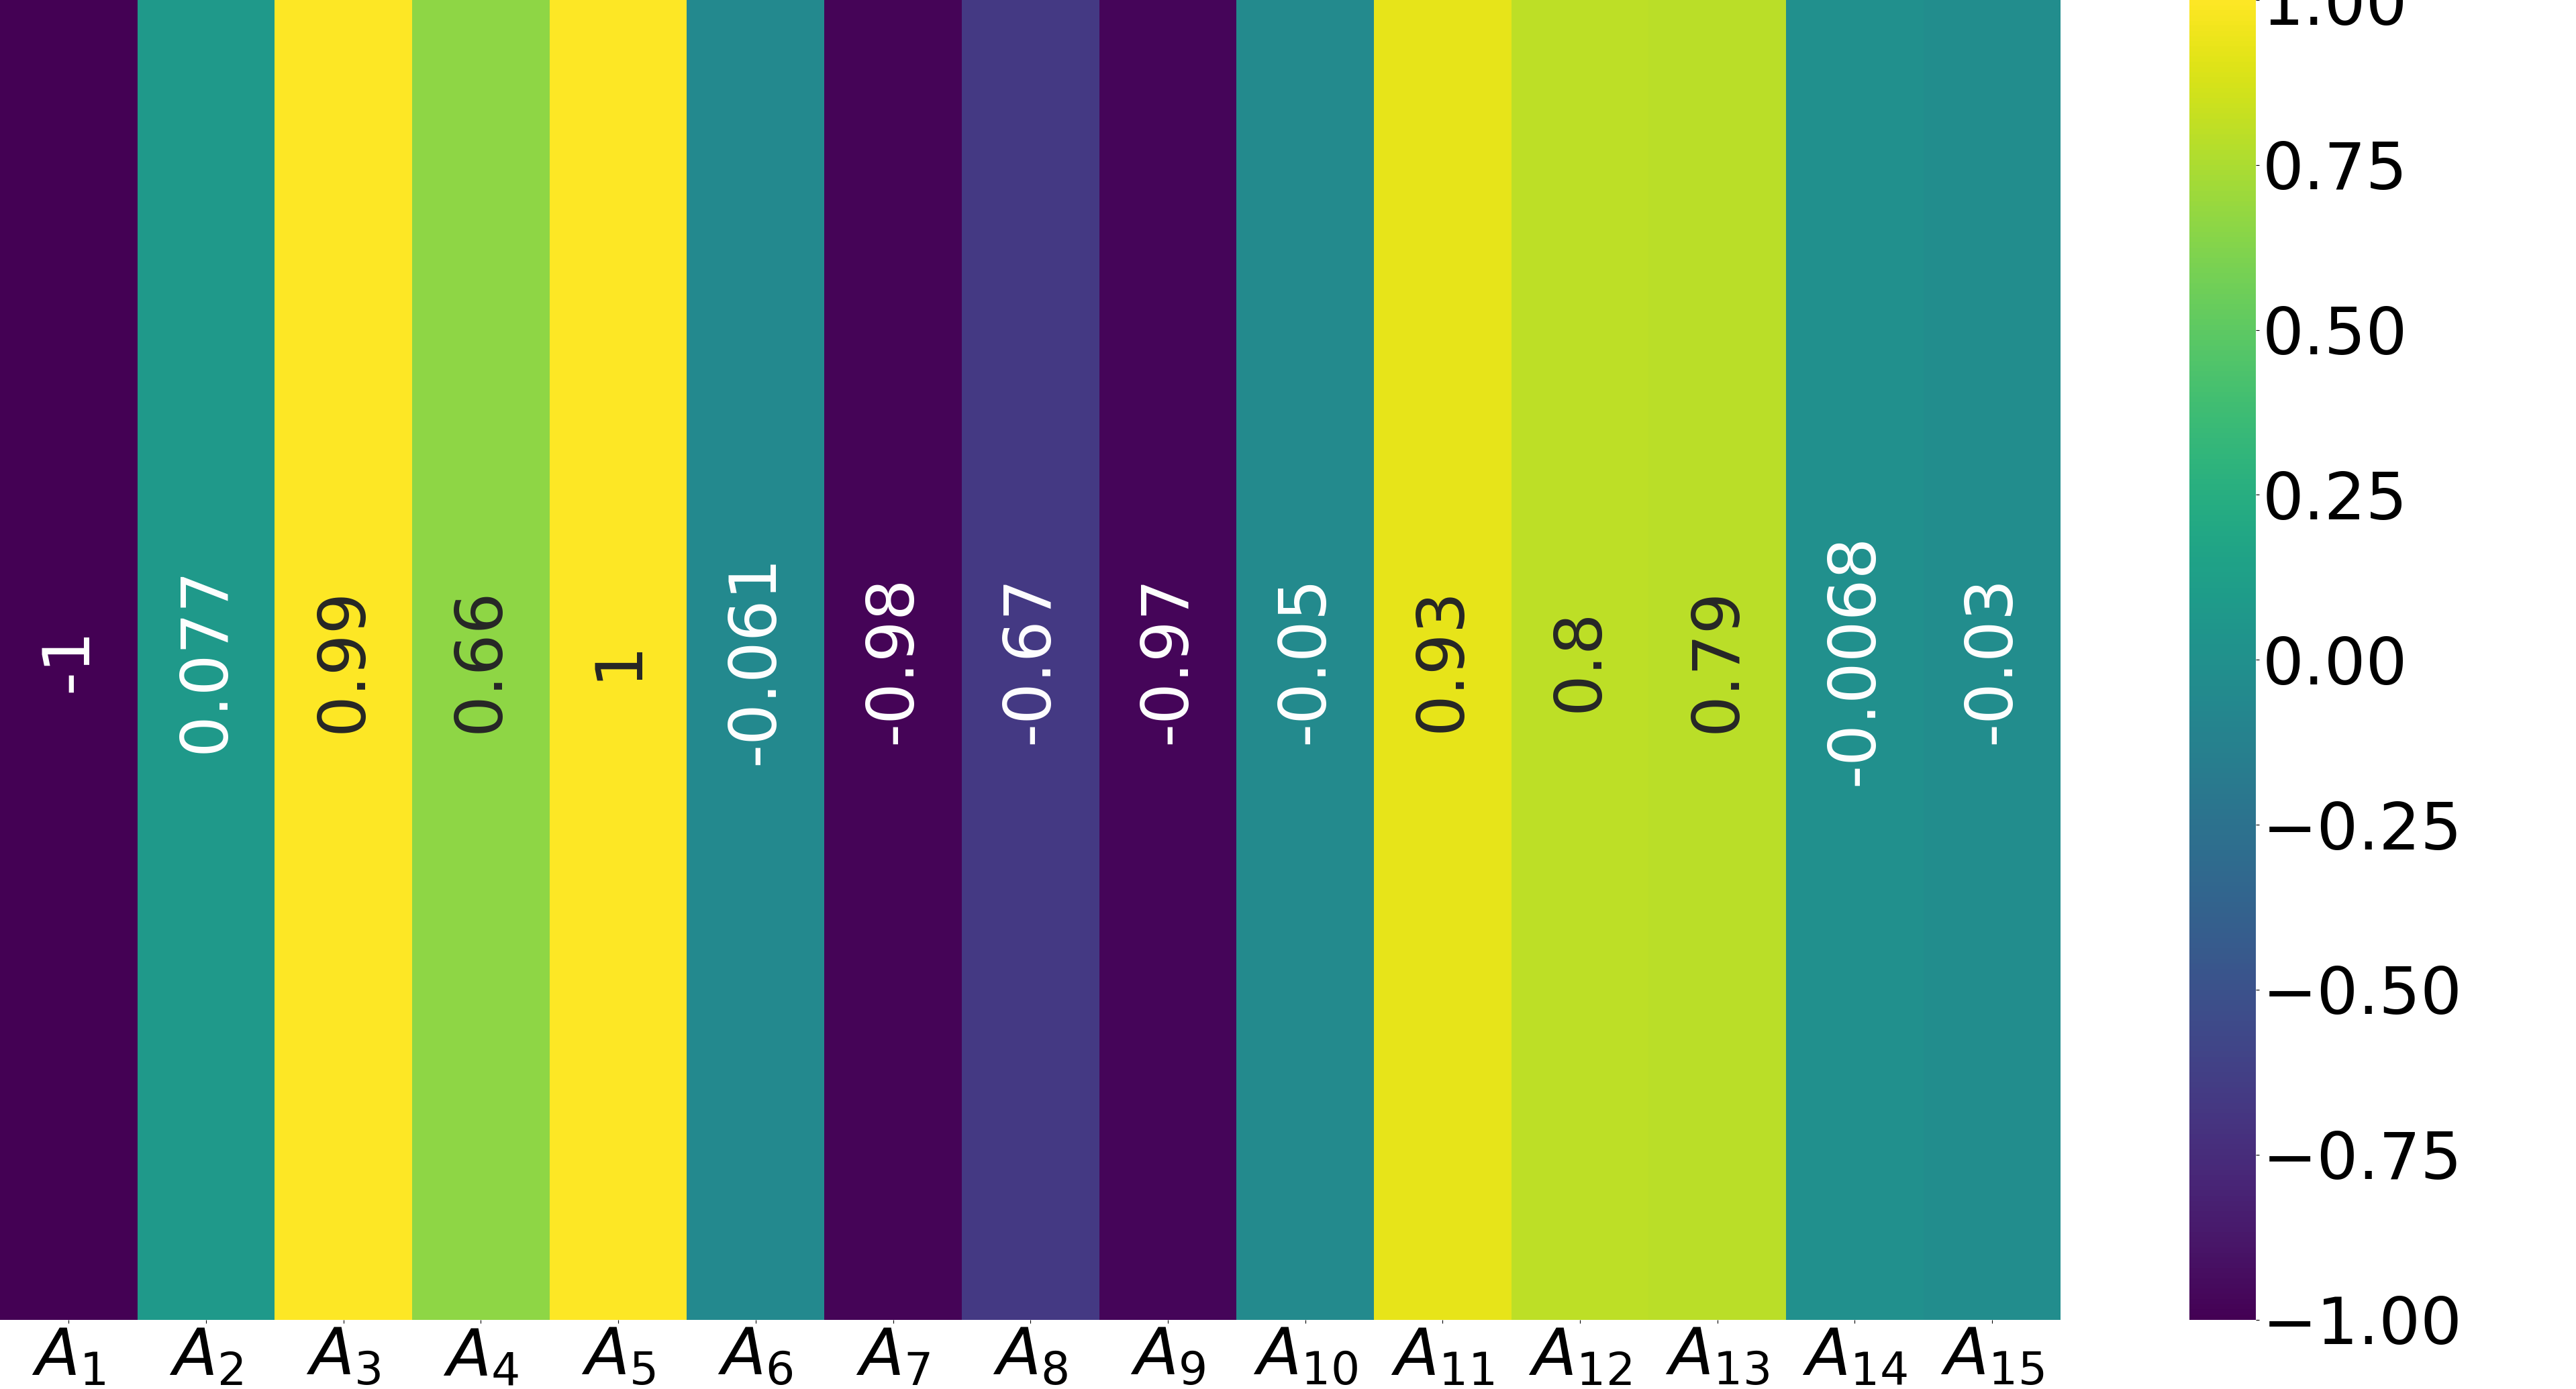
\includegraphics[width=\linewidth]{img/qlp_corr/An_coil0.png}
		\subcaption{Correlation with coil $0$}
	\end{subfigure}
	\begin{subfigure}{0.49\linewidth}
		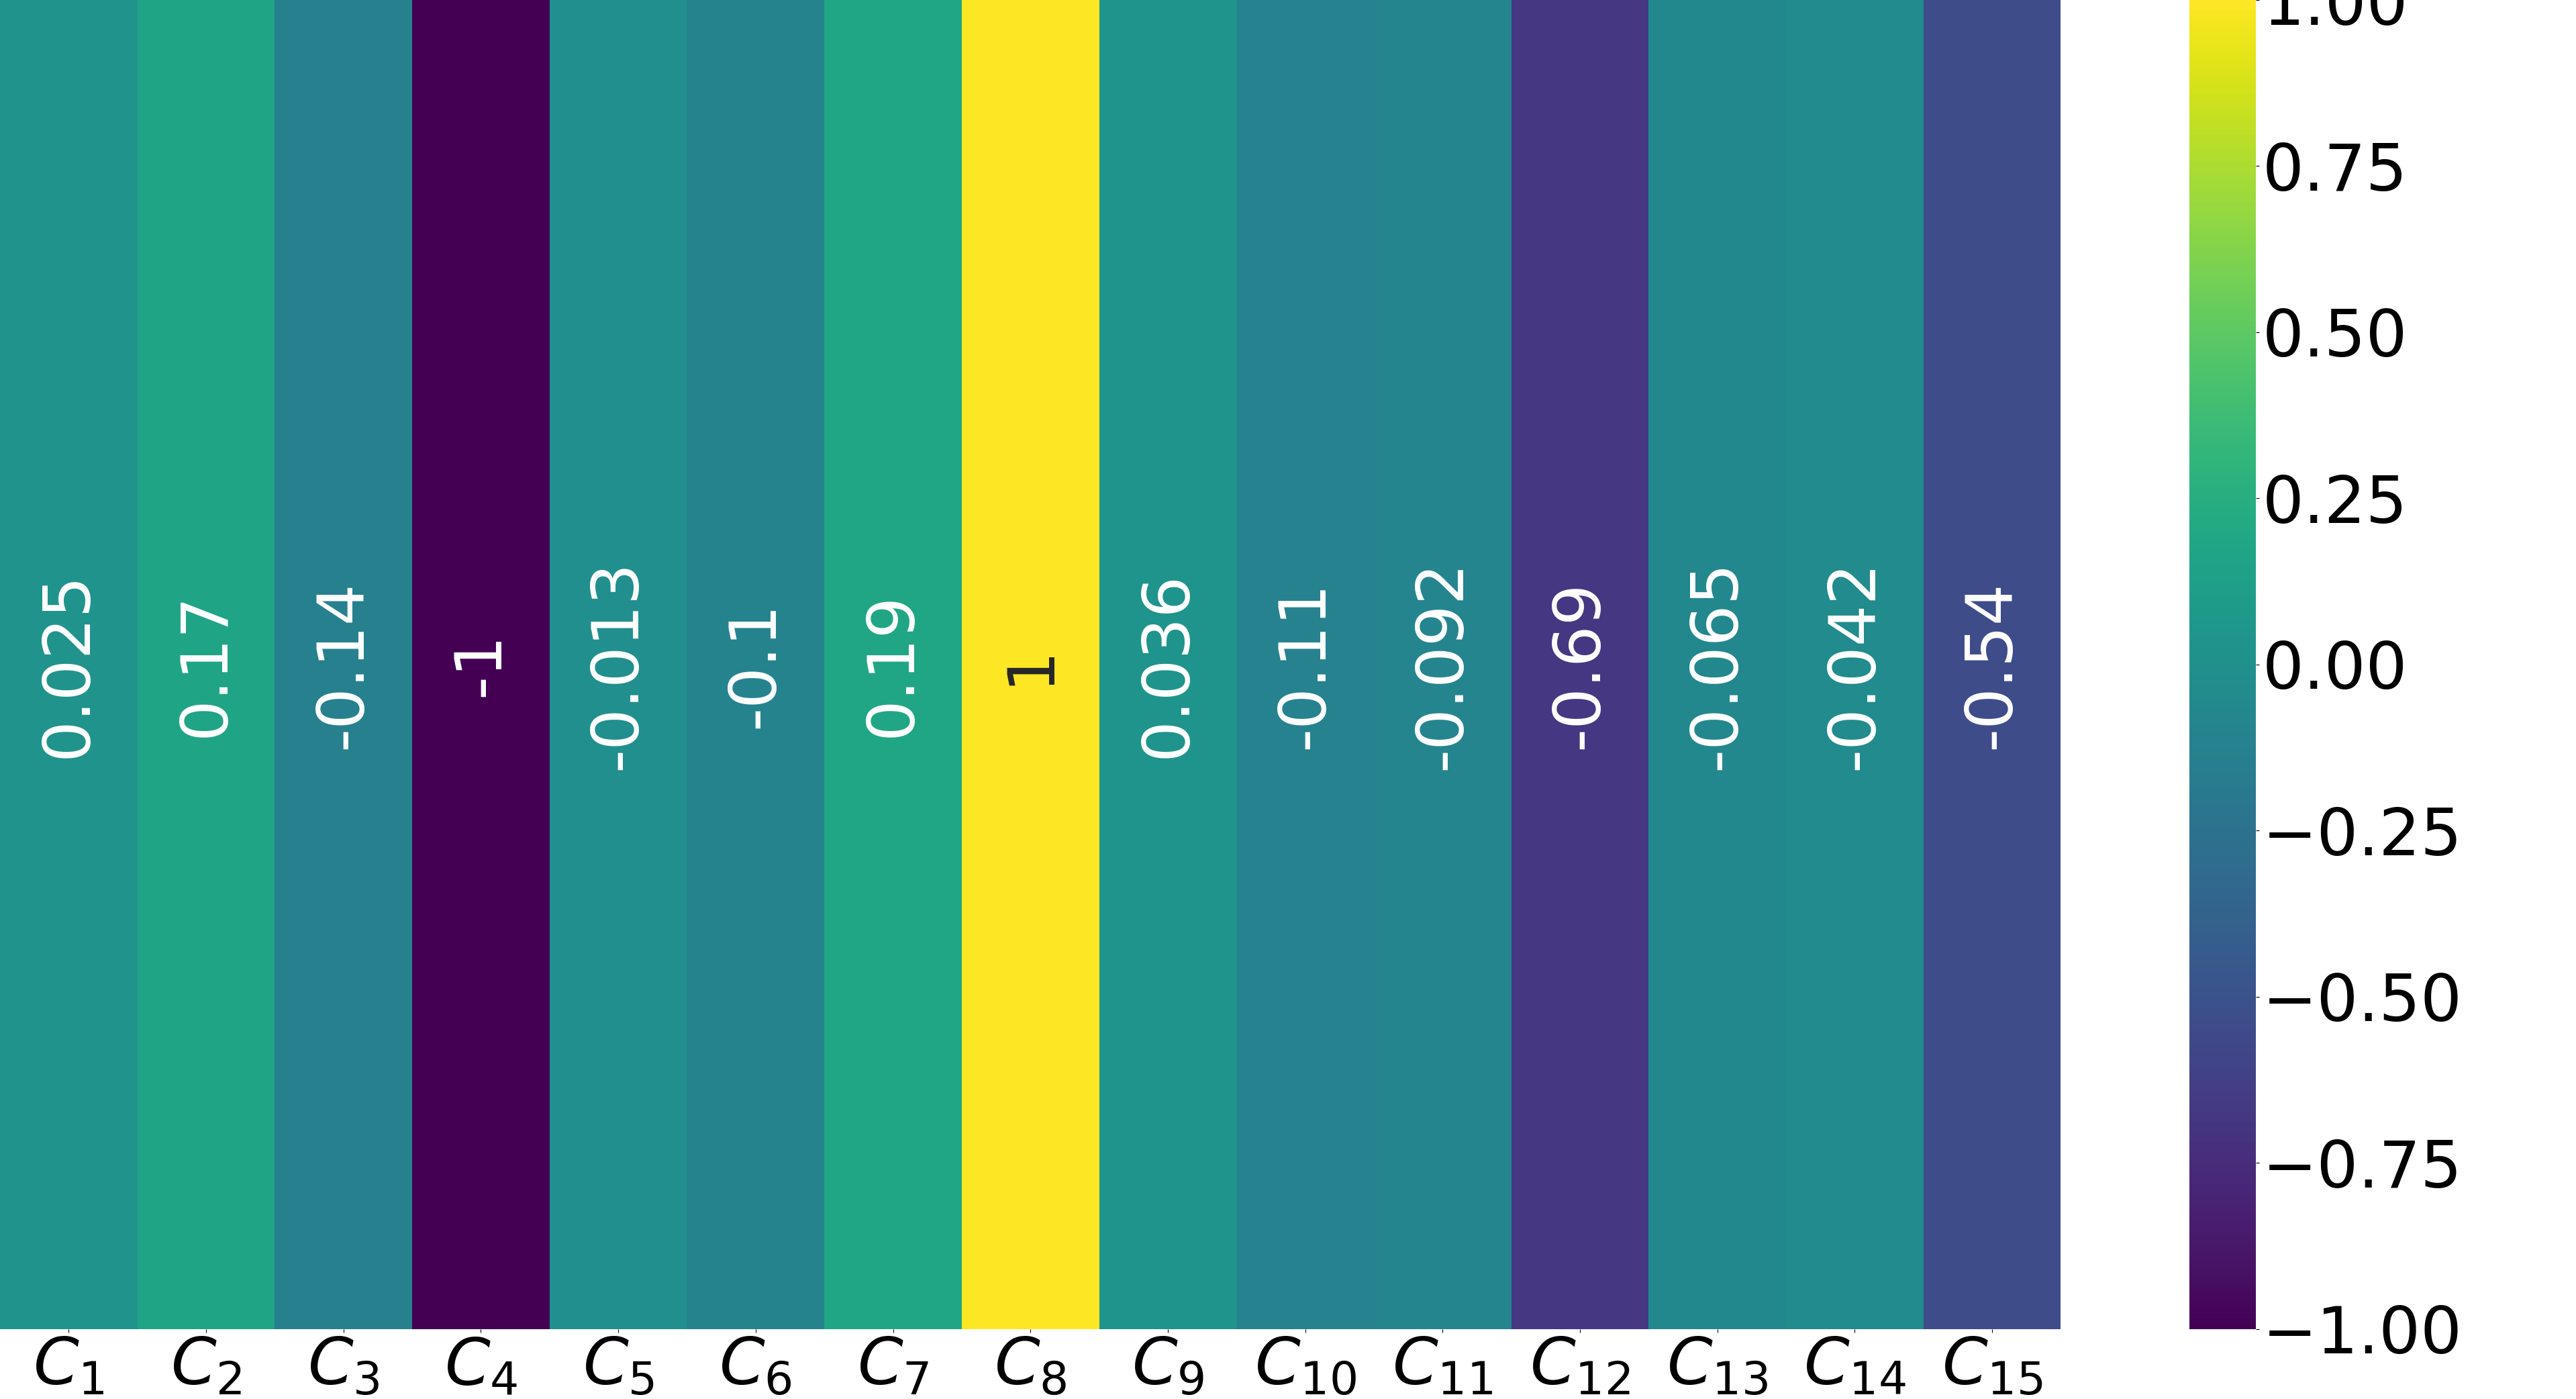
\includegraphics[width=\linewidth]{img/qlp_corr/An_coil1.png}
		\subcaption{Correlation with coil $1$}
	\end{subfigure}
	\begin{subfigure}{0.49\linewidth}
		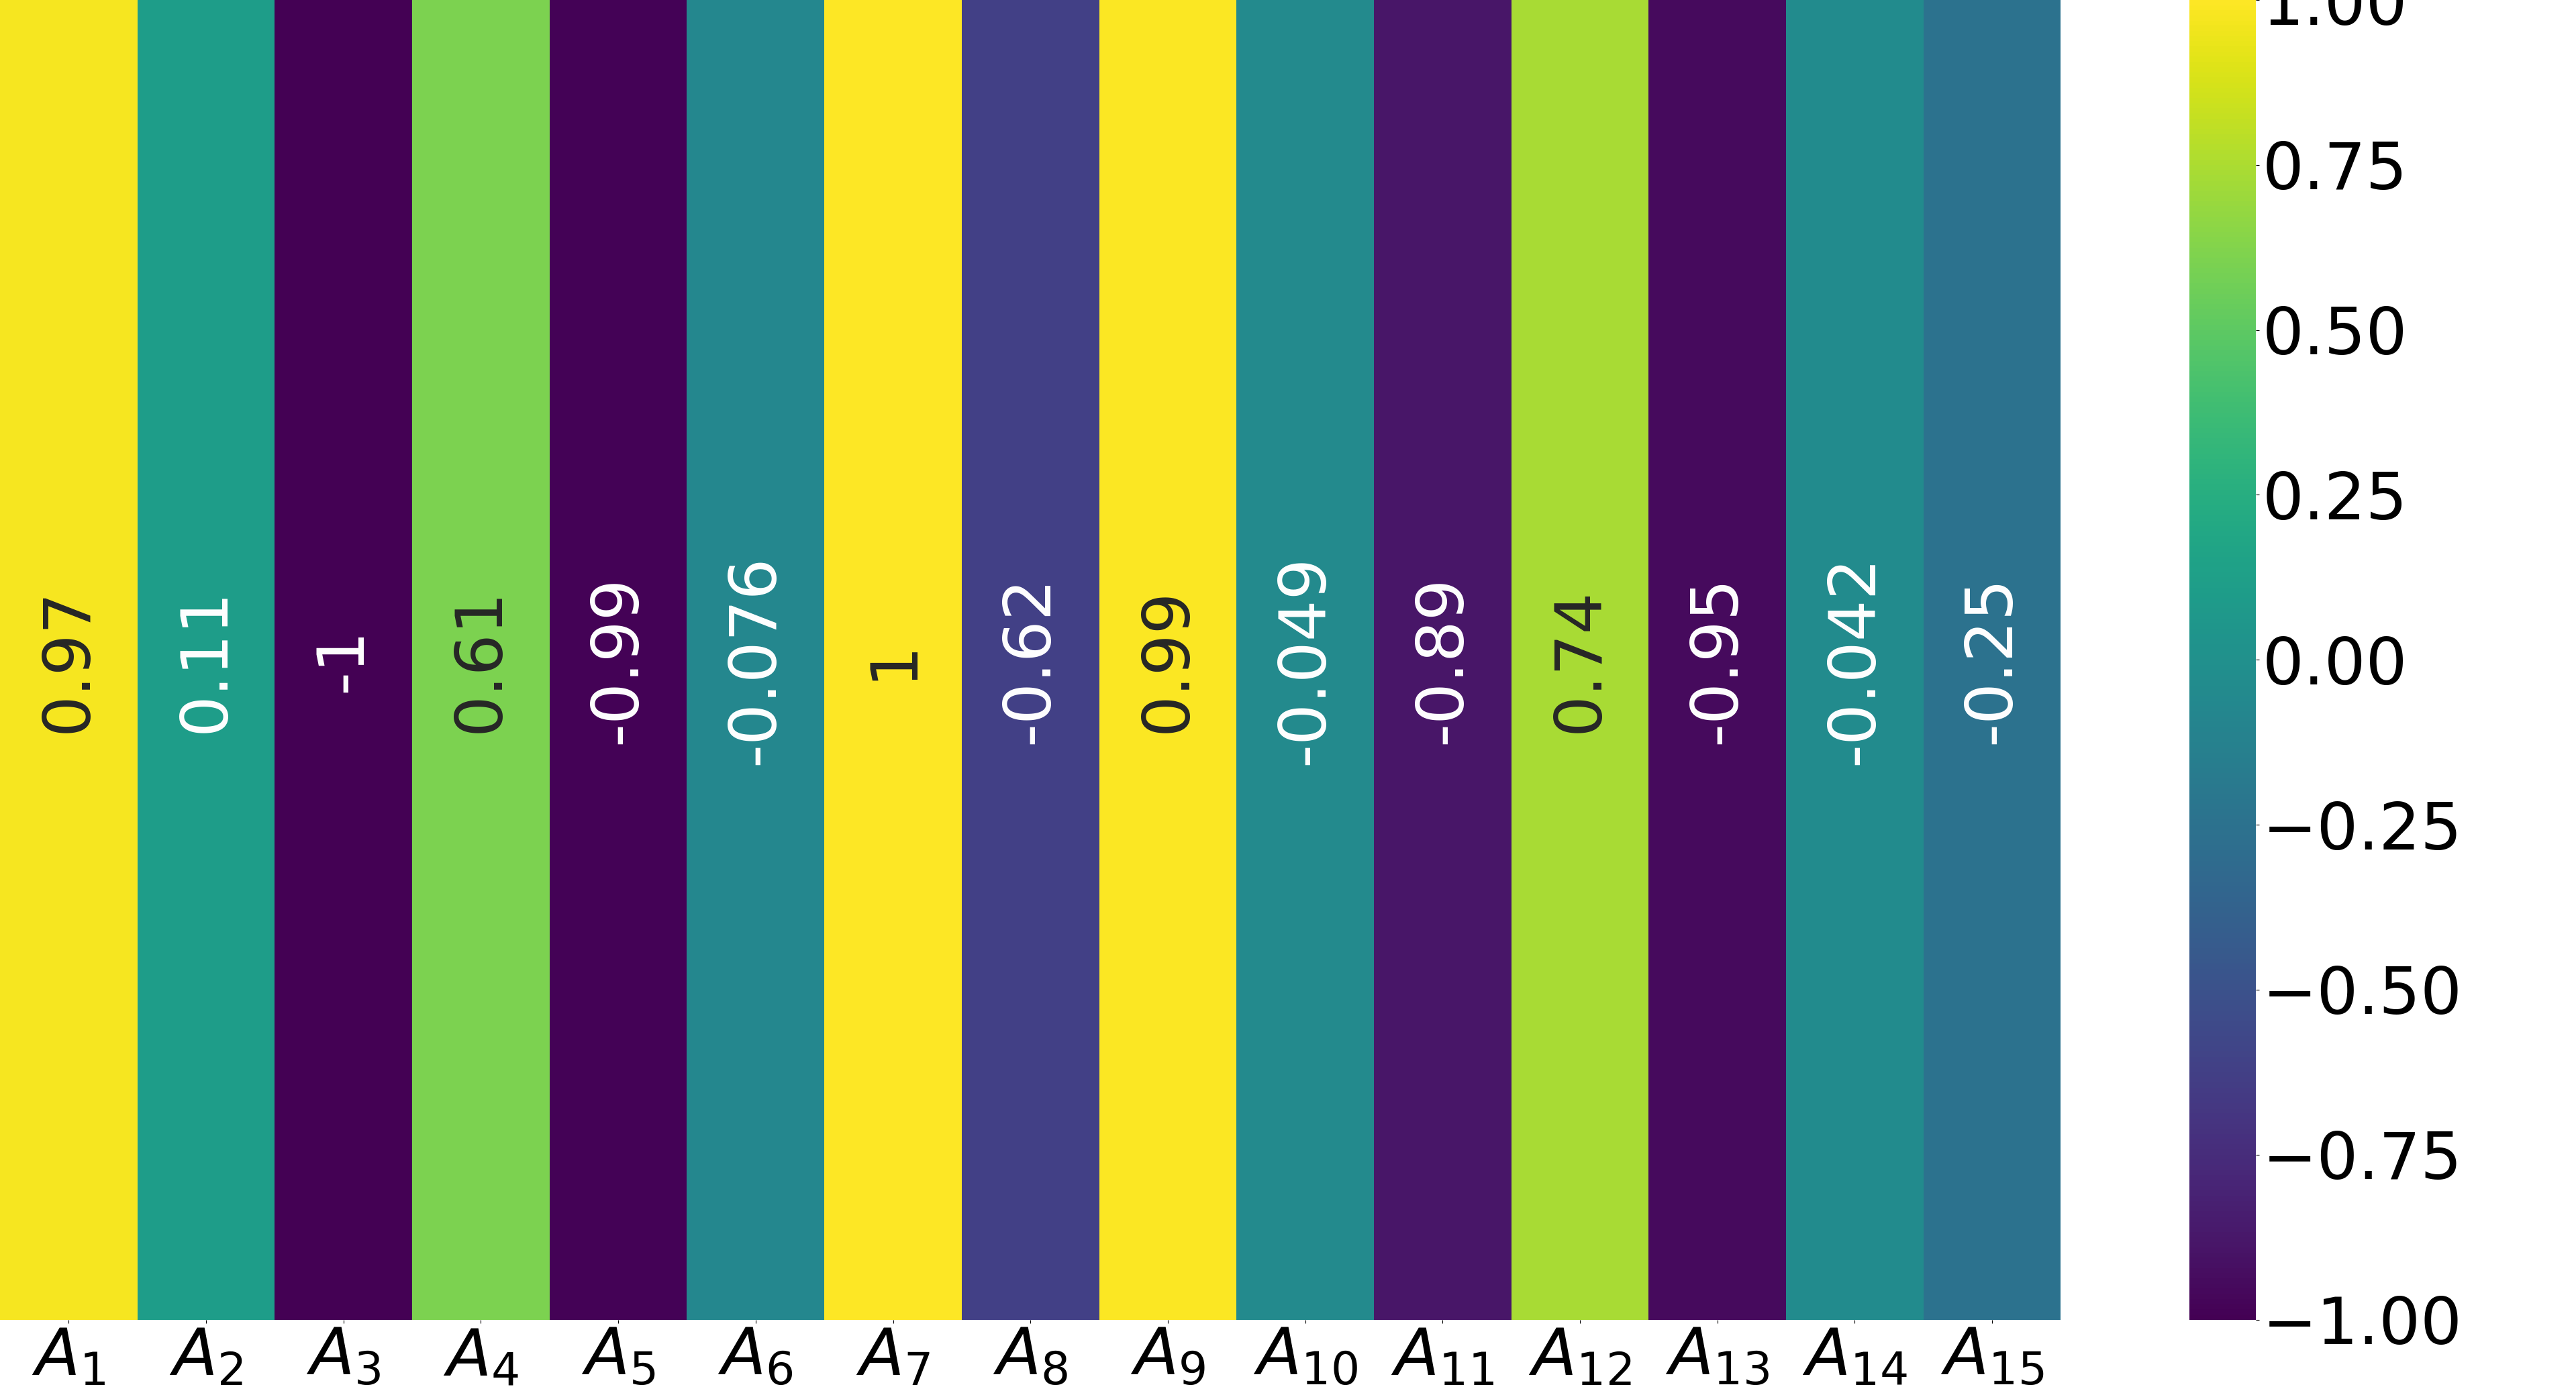
\includegraphics[width=\linewidth]{img/qlp_corr/An_coil2.png}
		\subcaption{Correlation with coil $2$}
	\end{subfigure}
	\begin{subfigure}{0.49\linewidth}
		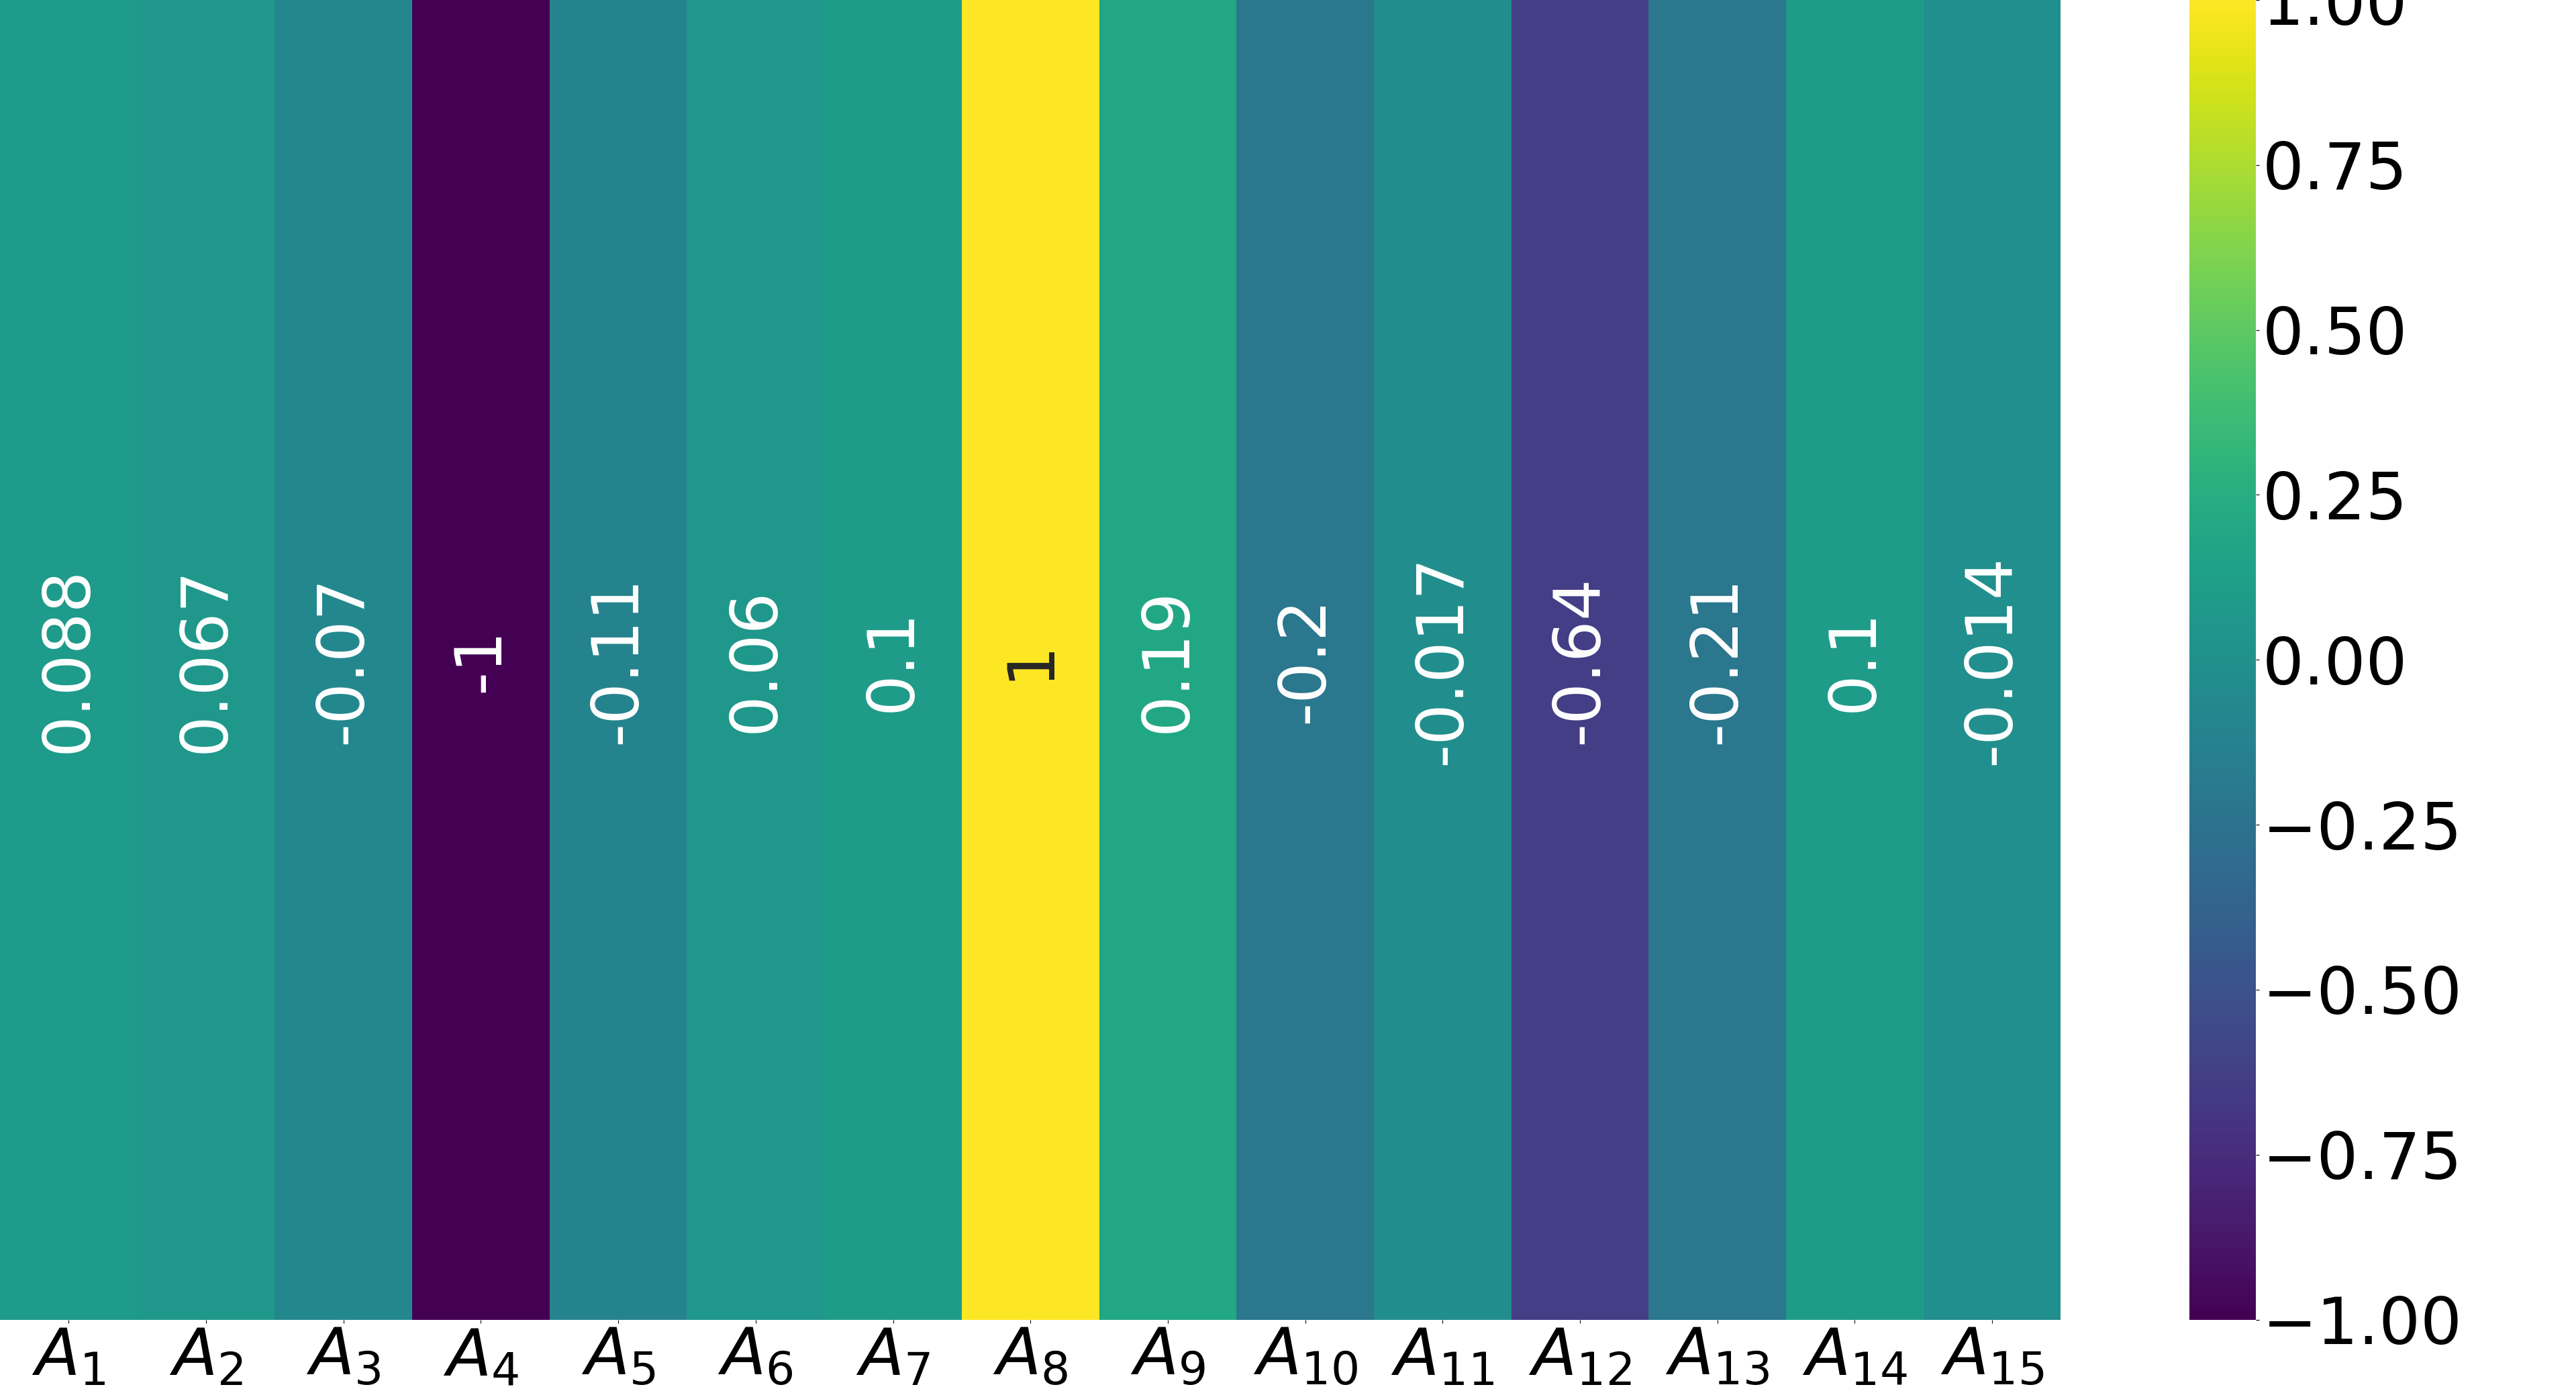
\includegraphics[width=\linewidth]{img/qlp_corr/An_coil3.png}
		\subcaption{Correlation with coil $3$}
	\end{subfigure}
	\caption{Correlation between the harmonics of the \an\ attribute and the labels for \qlp.}
	\label{fig:an-lcorr-qlp}
\end{figure}

In figure \Cref{fig:an-coilq-dist} we visualized the distribution of samples for \an\ in
bidimensional space, after a round of \pca\ dimensionality reduction. If we color the samples based
on the number of coils quenched for that specific sample ($0, 1, \geq 1$), as shown in sub-figure
(a), we can easily identify and label clusters with a high level of purity. If we color samples
based on whether a specific coil quenched or not (sub-figures (b) through (e)), it's quite clear that it's not
as easy to find clusters that contain only samples labelled as quench, especially in the case of
coils $1$, sub-figure (c), and $3$, sub-figure (e).

A less-than-ideal distribution of the samples in bidimensional space was expected due to the poor
correlation between the attribute and the labels for coils $1$ and $3$ highlighted in \Cref{fig:an-lcorr-qlp}.

\begin{figure}[!ht]
	% Font size = 70
	\centering
	\begin{subfigure}{\linewidth}
		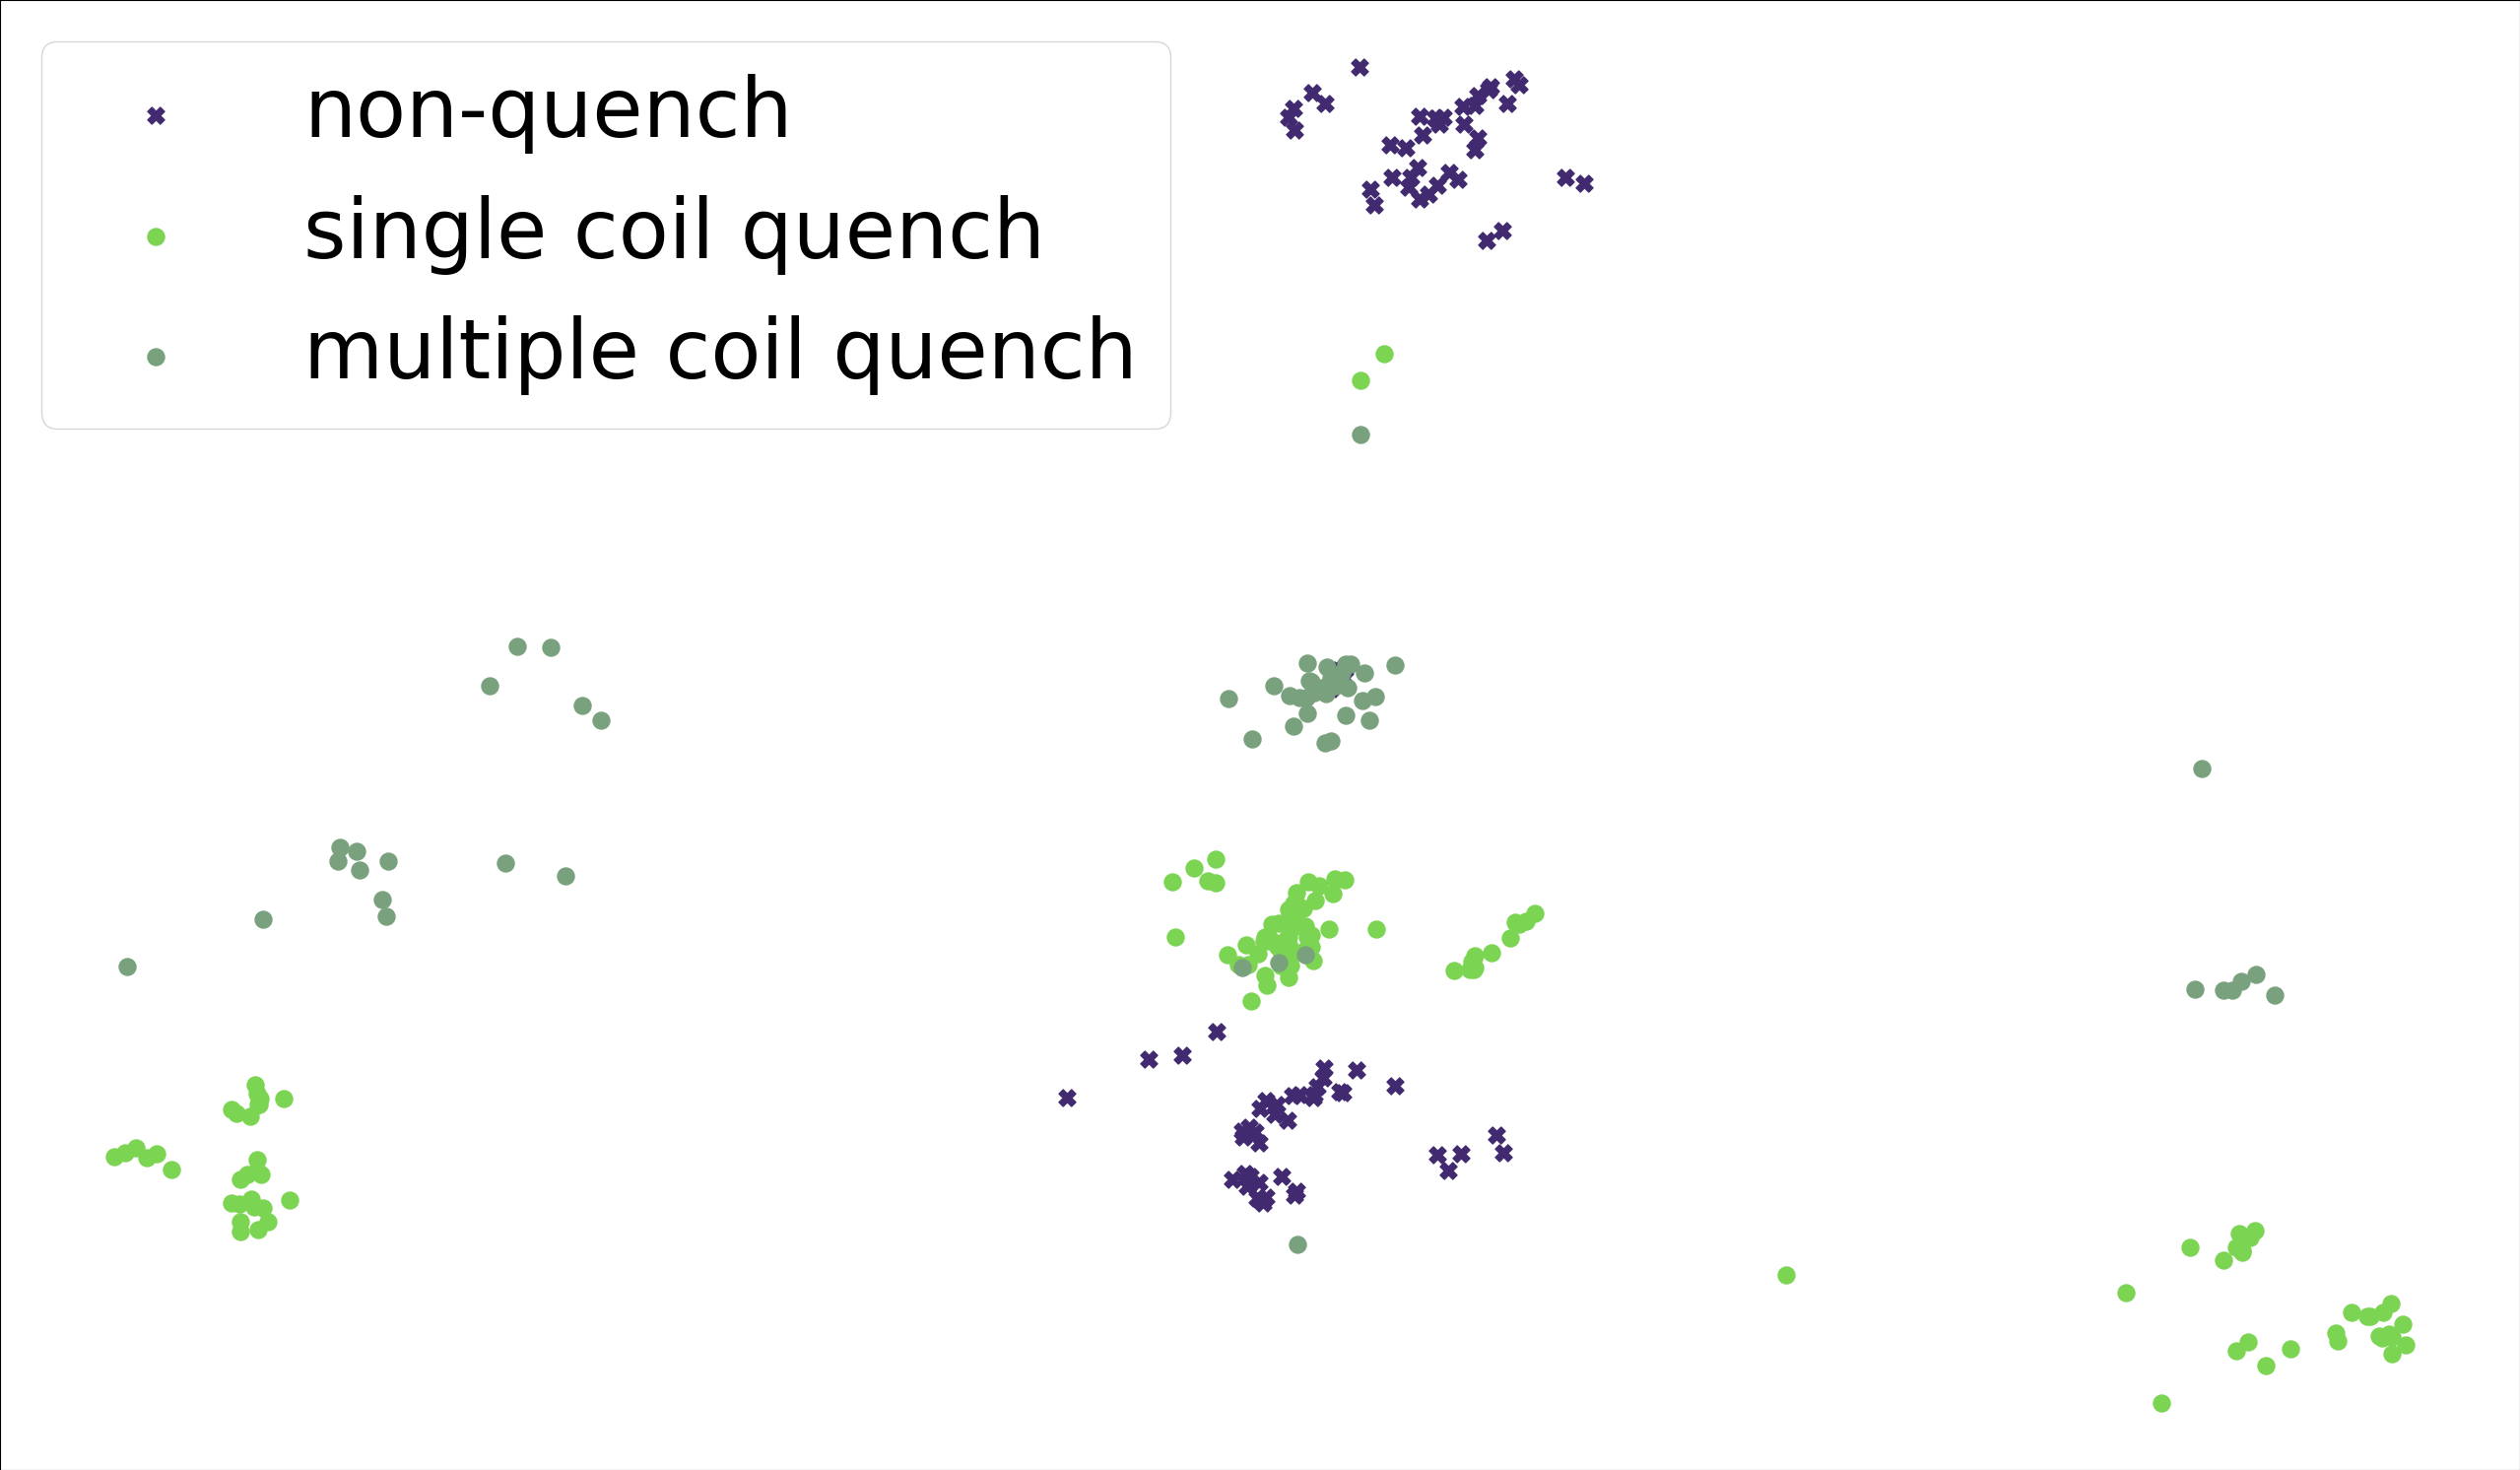
\includegraphics[width=\linewidth]{img/quench_dist_qlp/single_vs_multiple_An.png}
		\subcaption{}
	\end{subfigure}
	\begin{subfigure}{0.49\linewidth}
		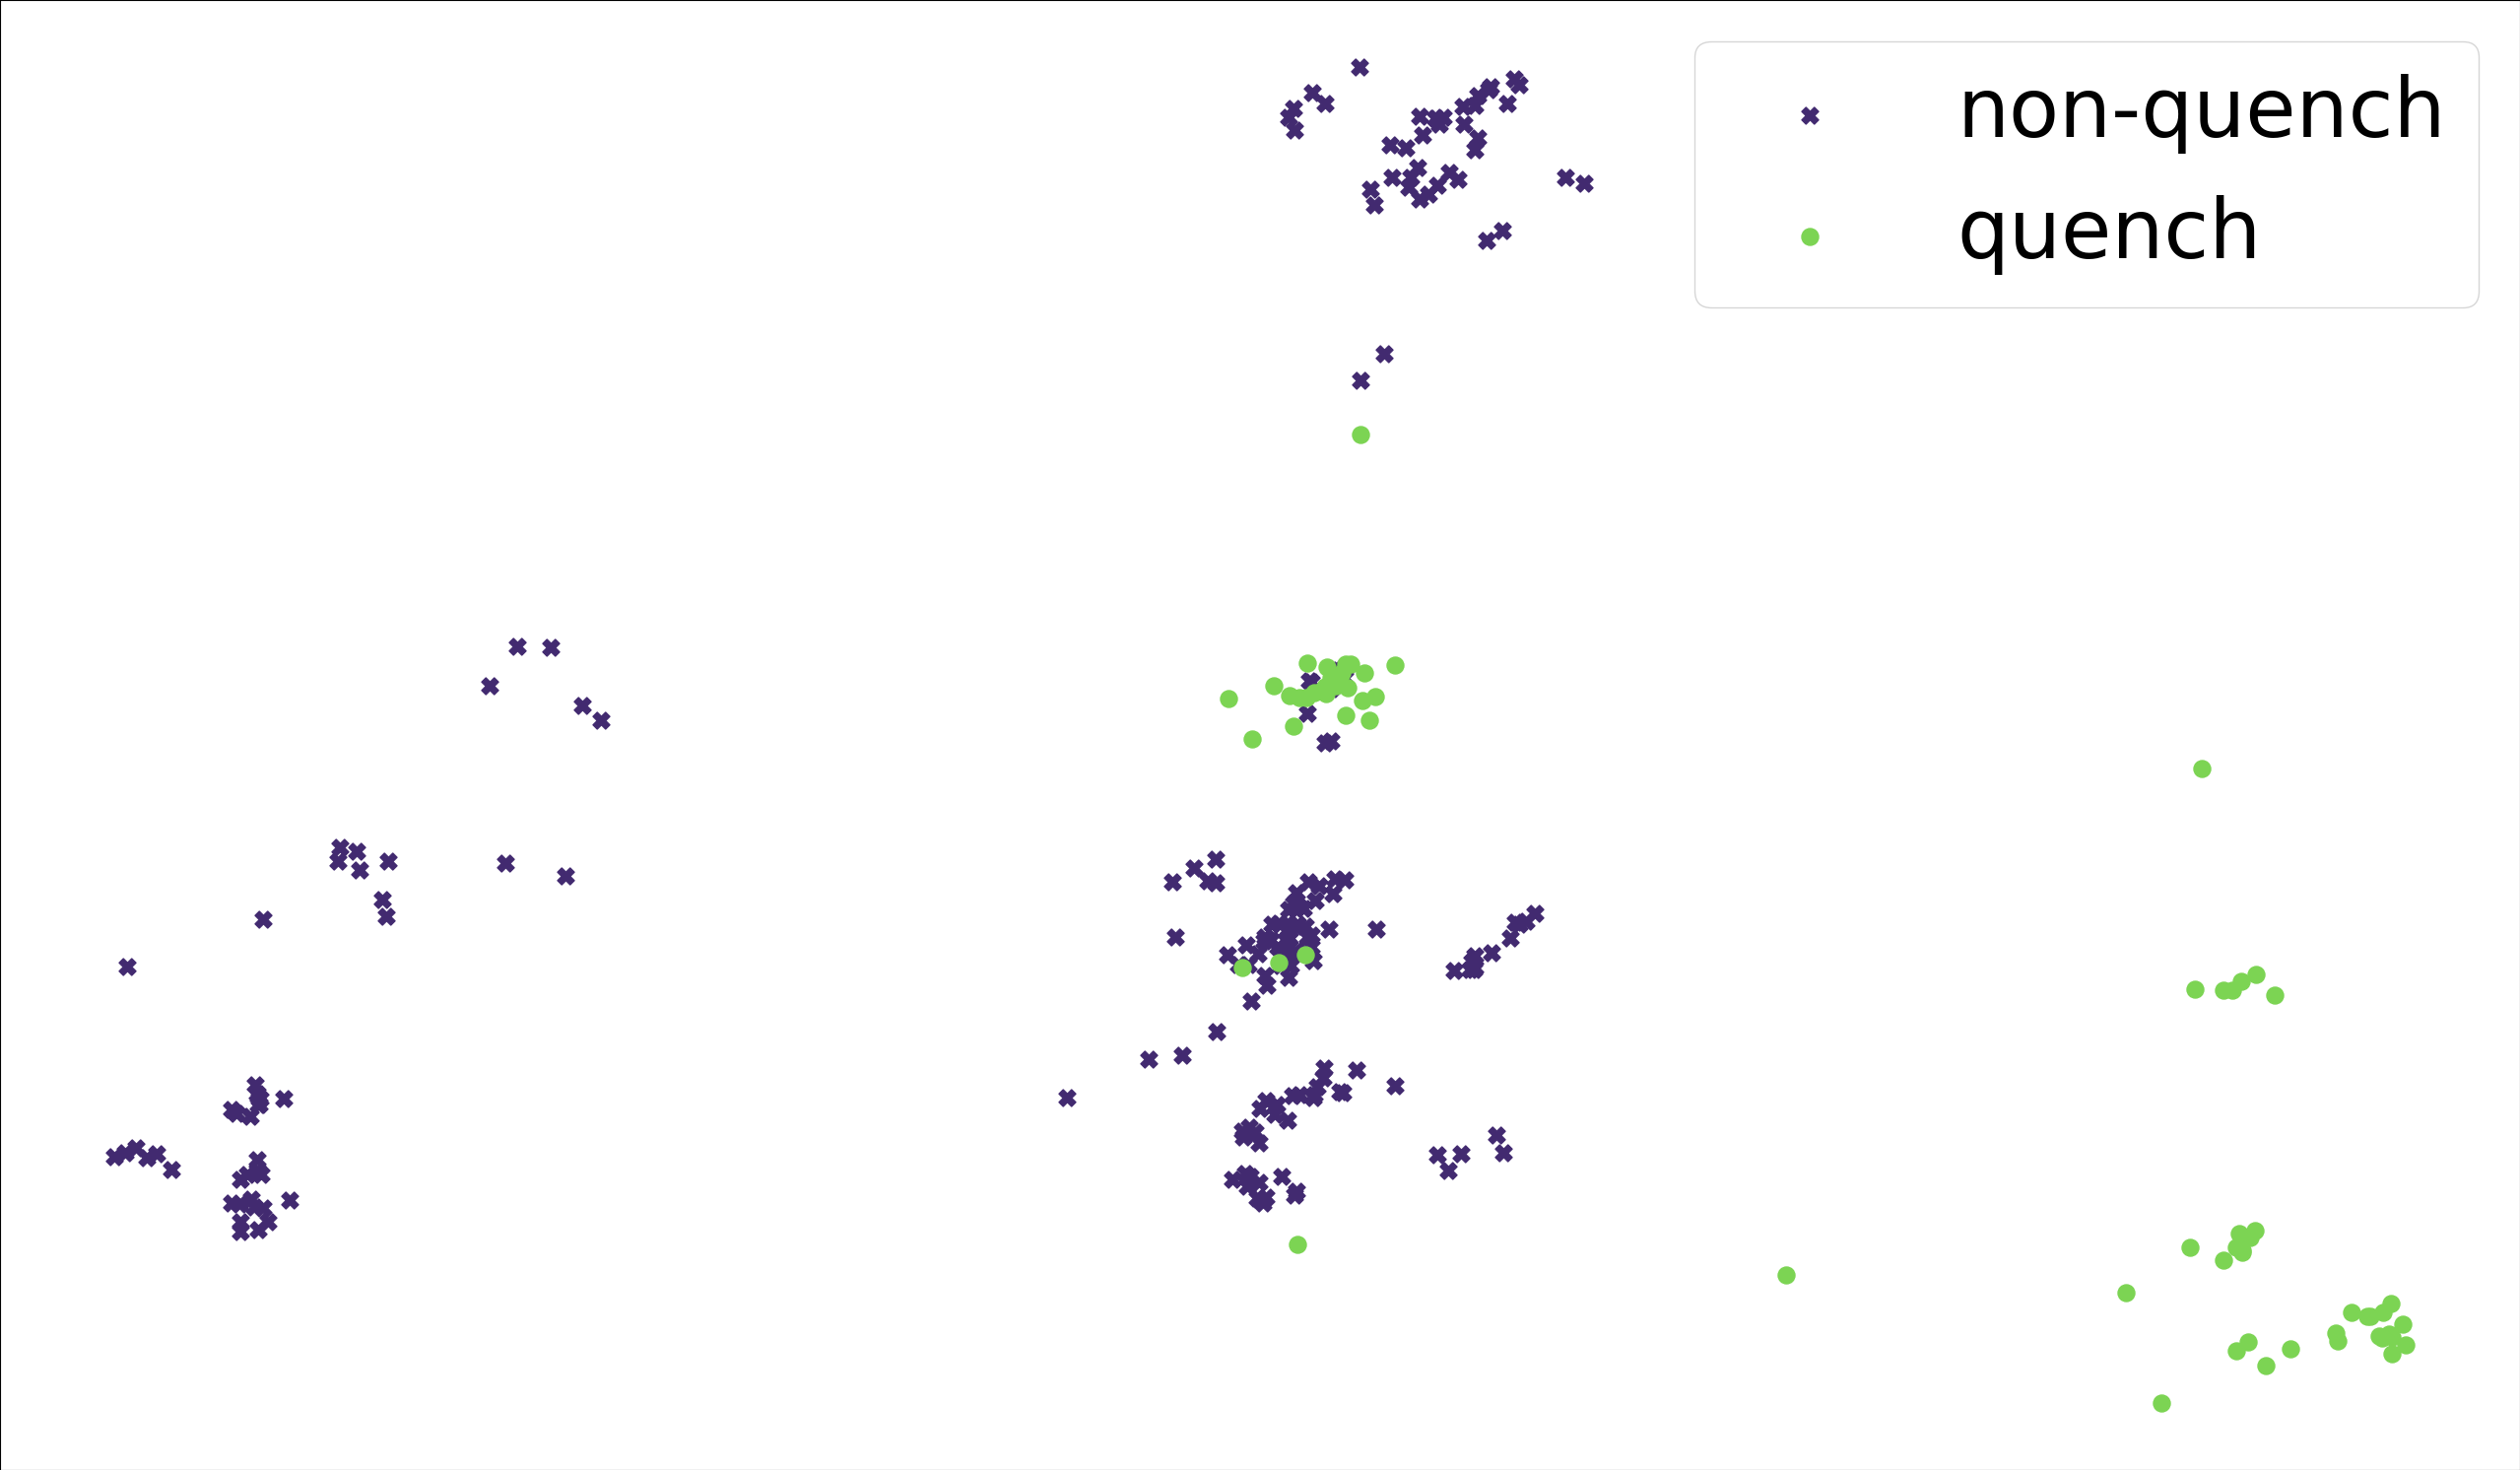
\includegraphics[width=\linewidth]{img/quench_dist_qlp/quenches_coil_0_An.png}
		\subcaption{}
	\end{subfigure}
	\begin{subfigure}{0.49\linewidth}
		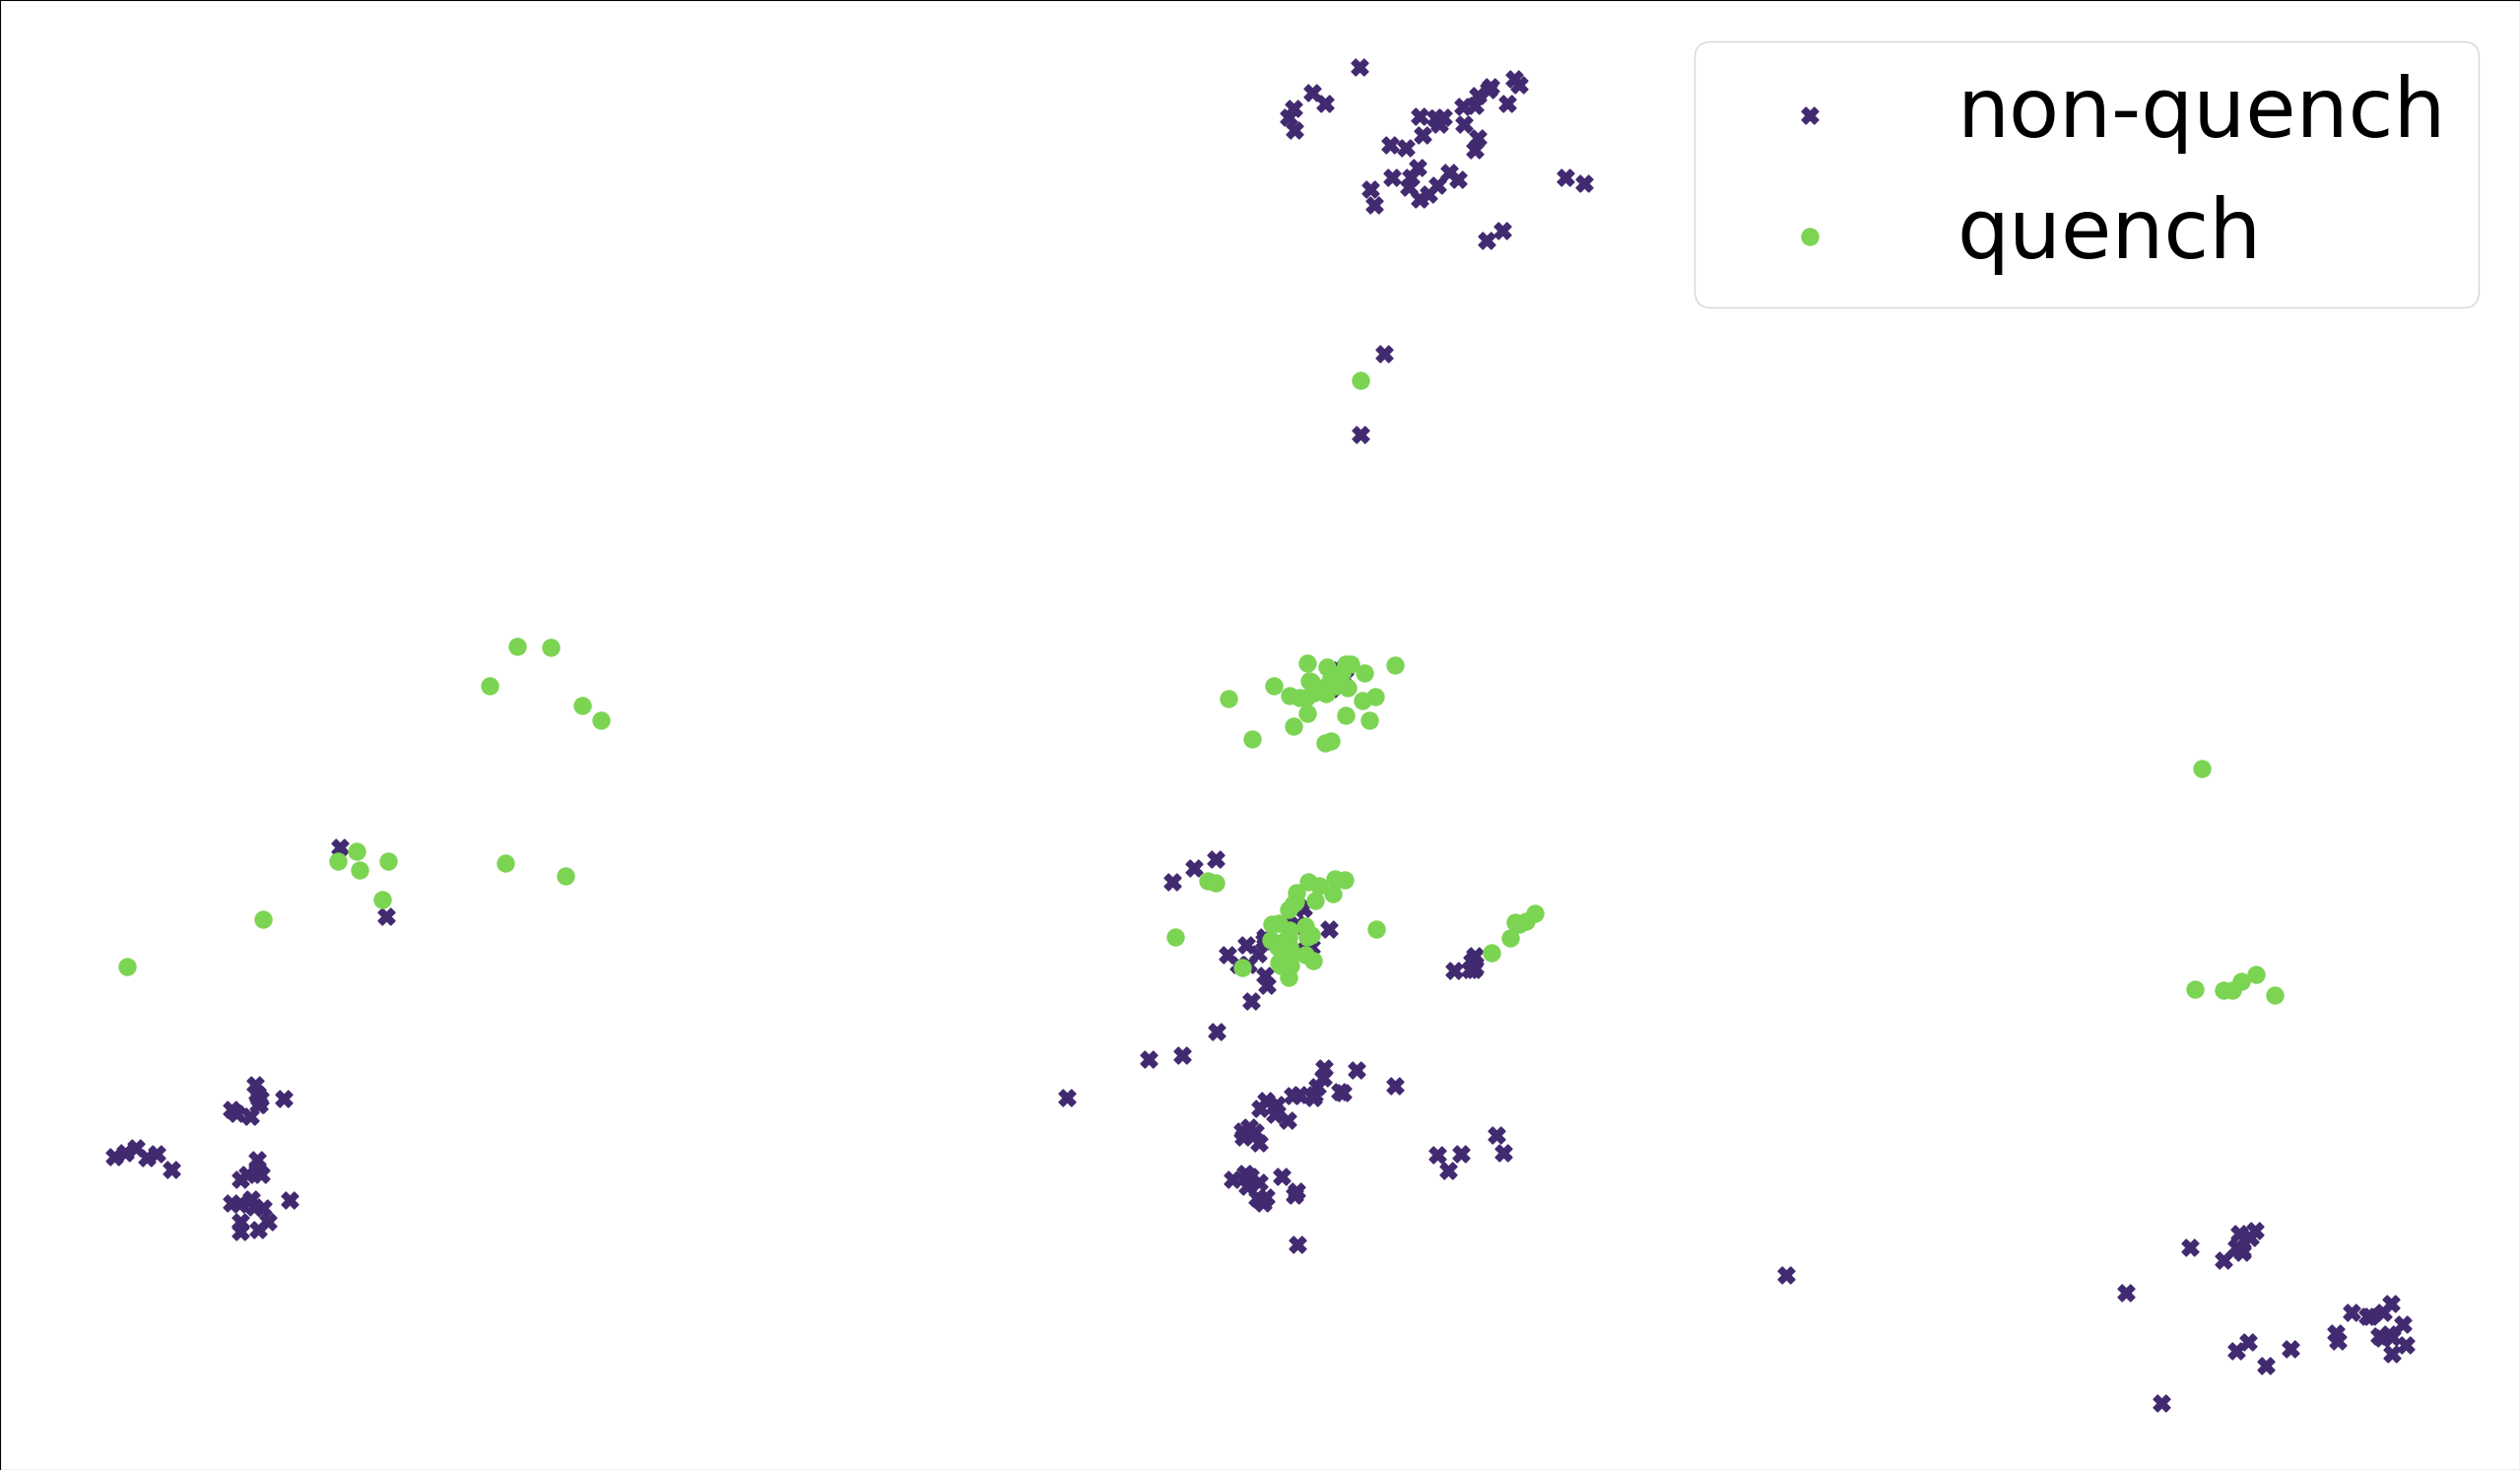
\includegraphics[width=\linewidth]{img/quench_dist_qlp/quenches_coil_1_An.png}
		\subcaption{}
	\end{subfigure}
	\begin{subfigure}{0.49\linewidth}
		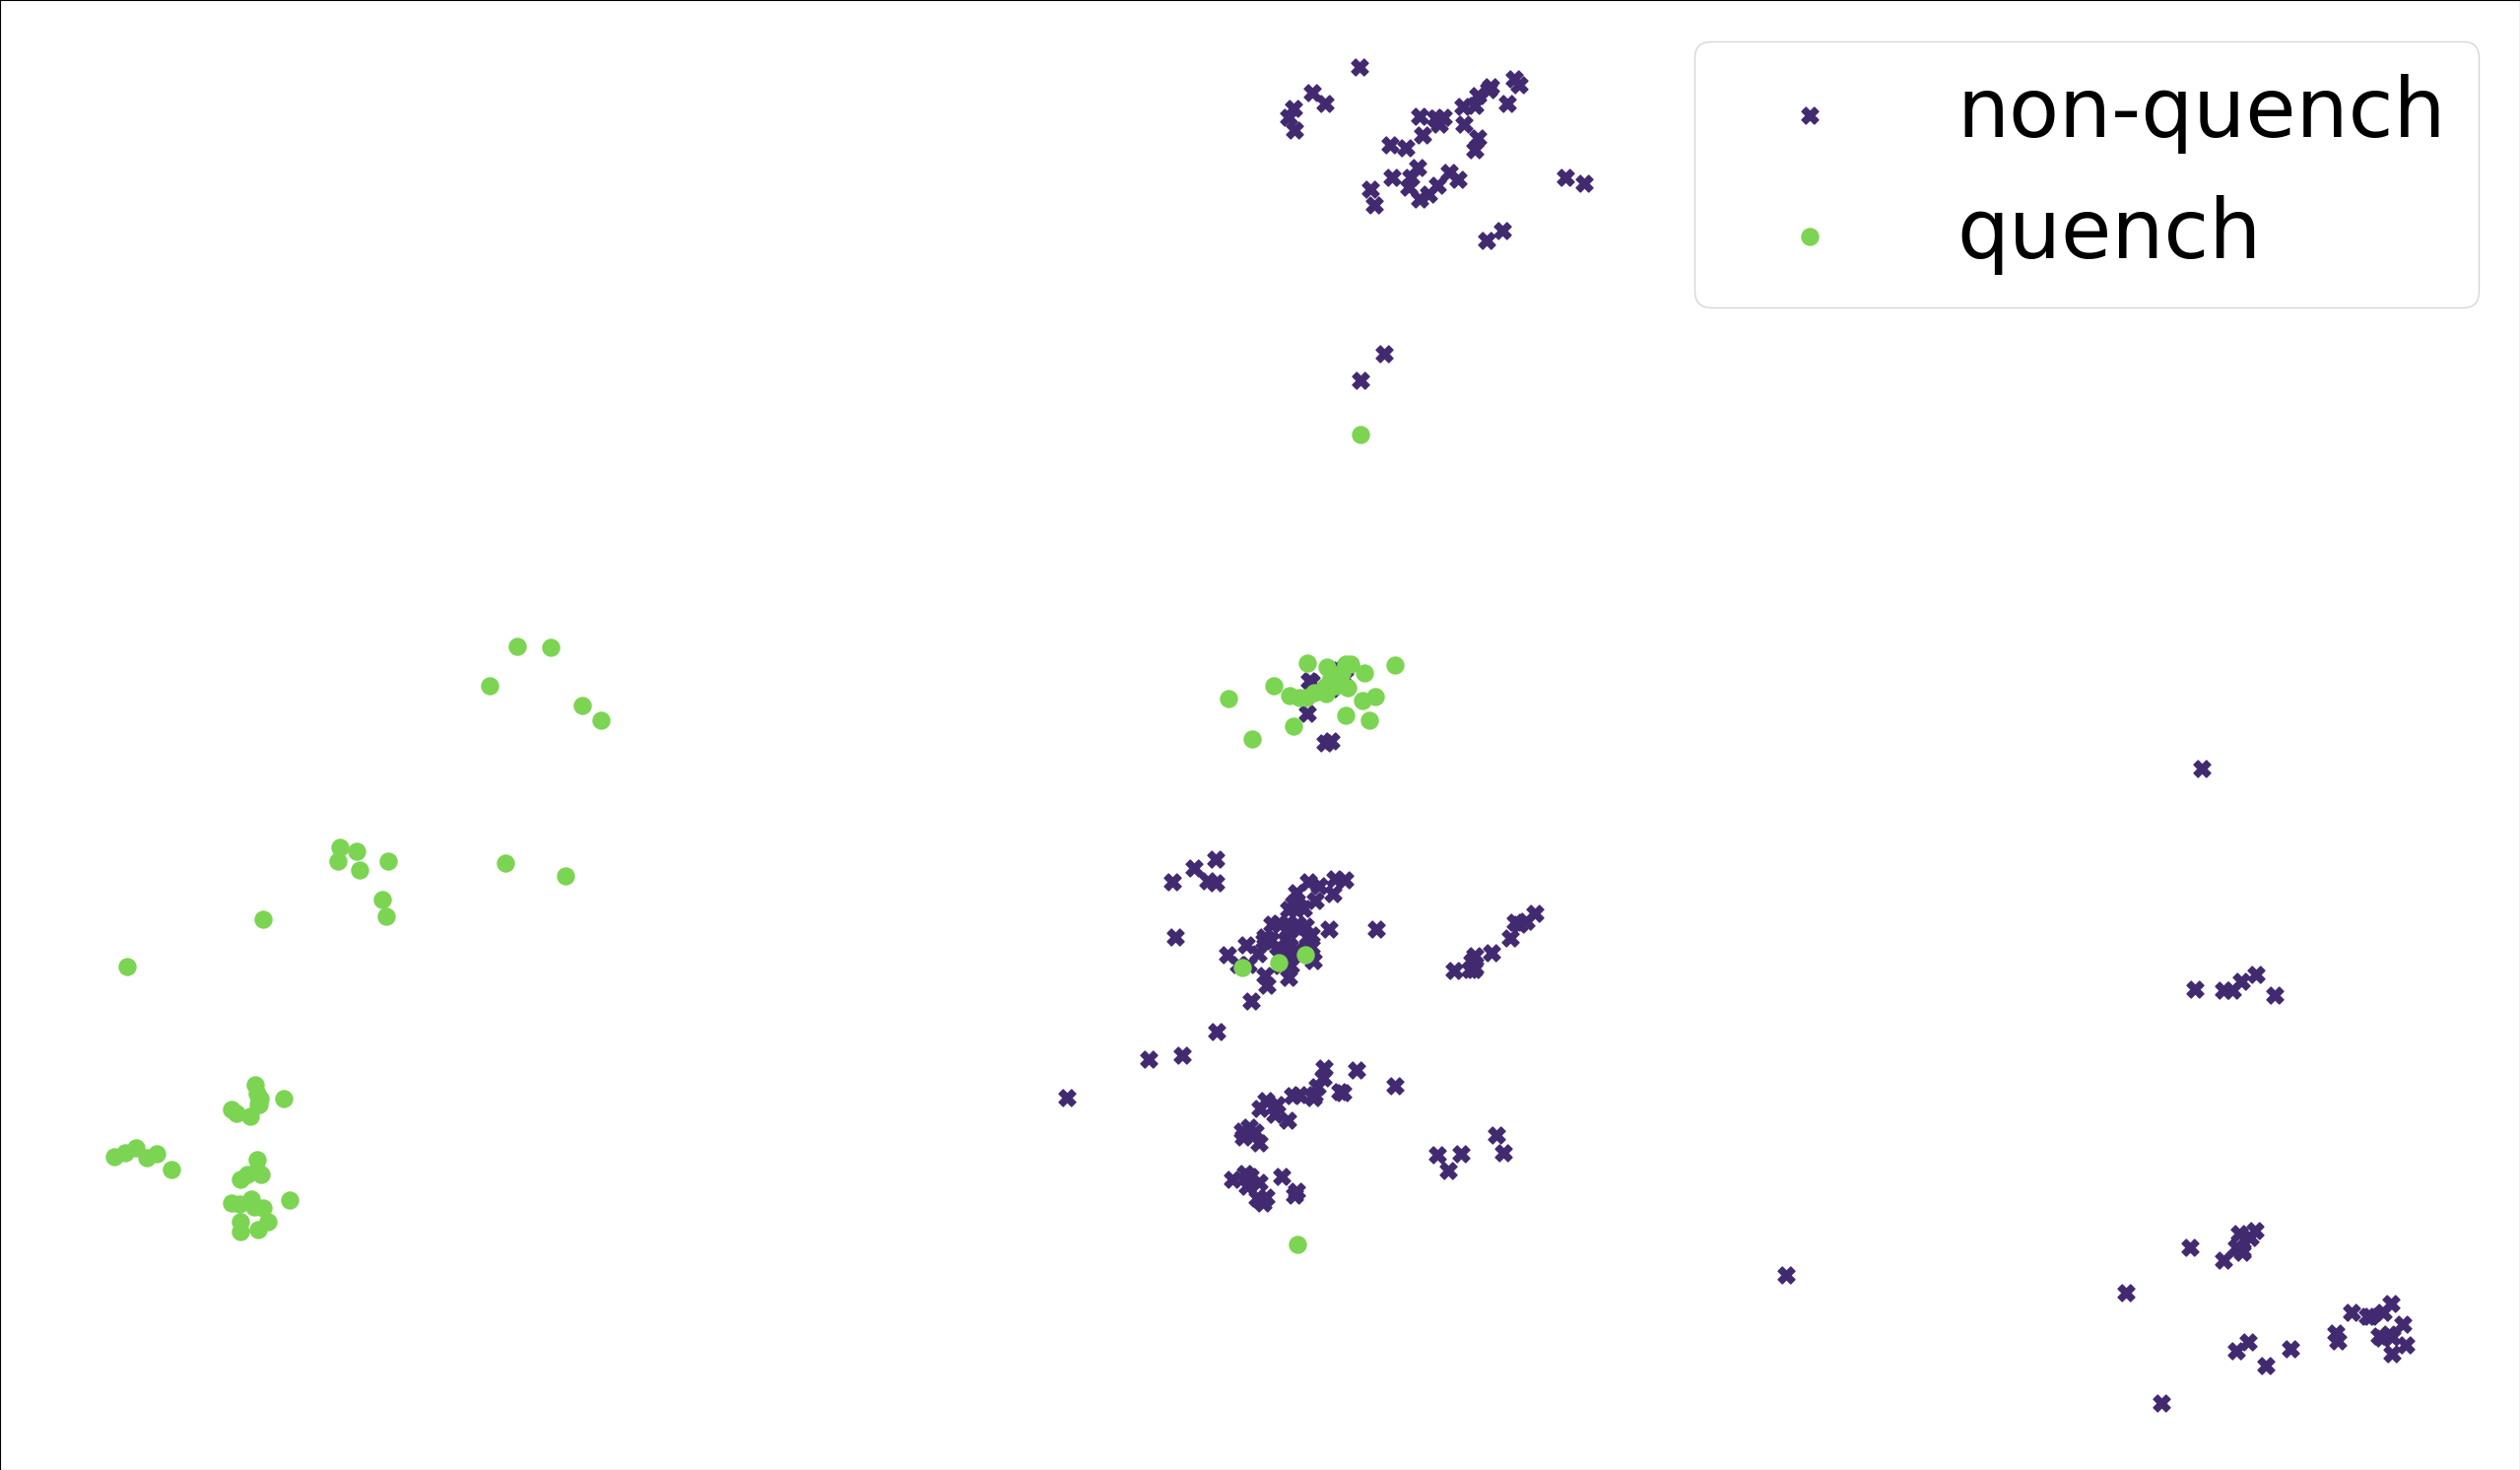
\includegraphics[width=\linewidth]{img/quench_dist_qlp/quenches_coil_2_An.png}
		\subcaption{}
	\end{subfigure}
	\begin{subfigure}{0.49\linewidth}
		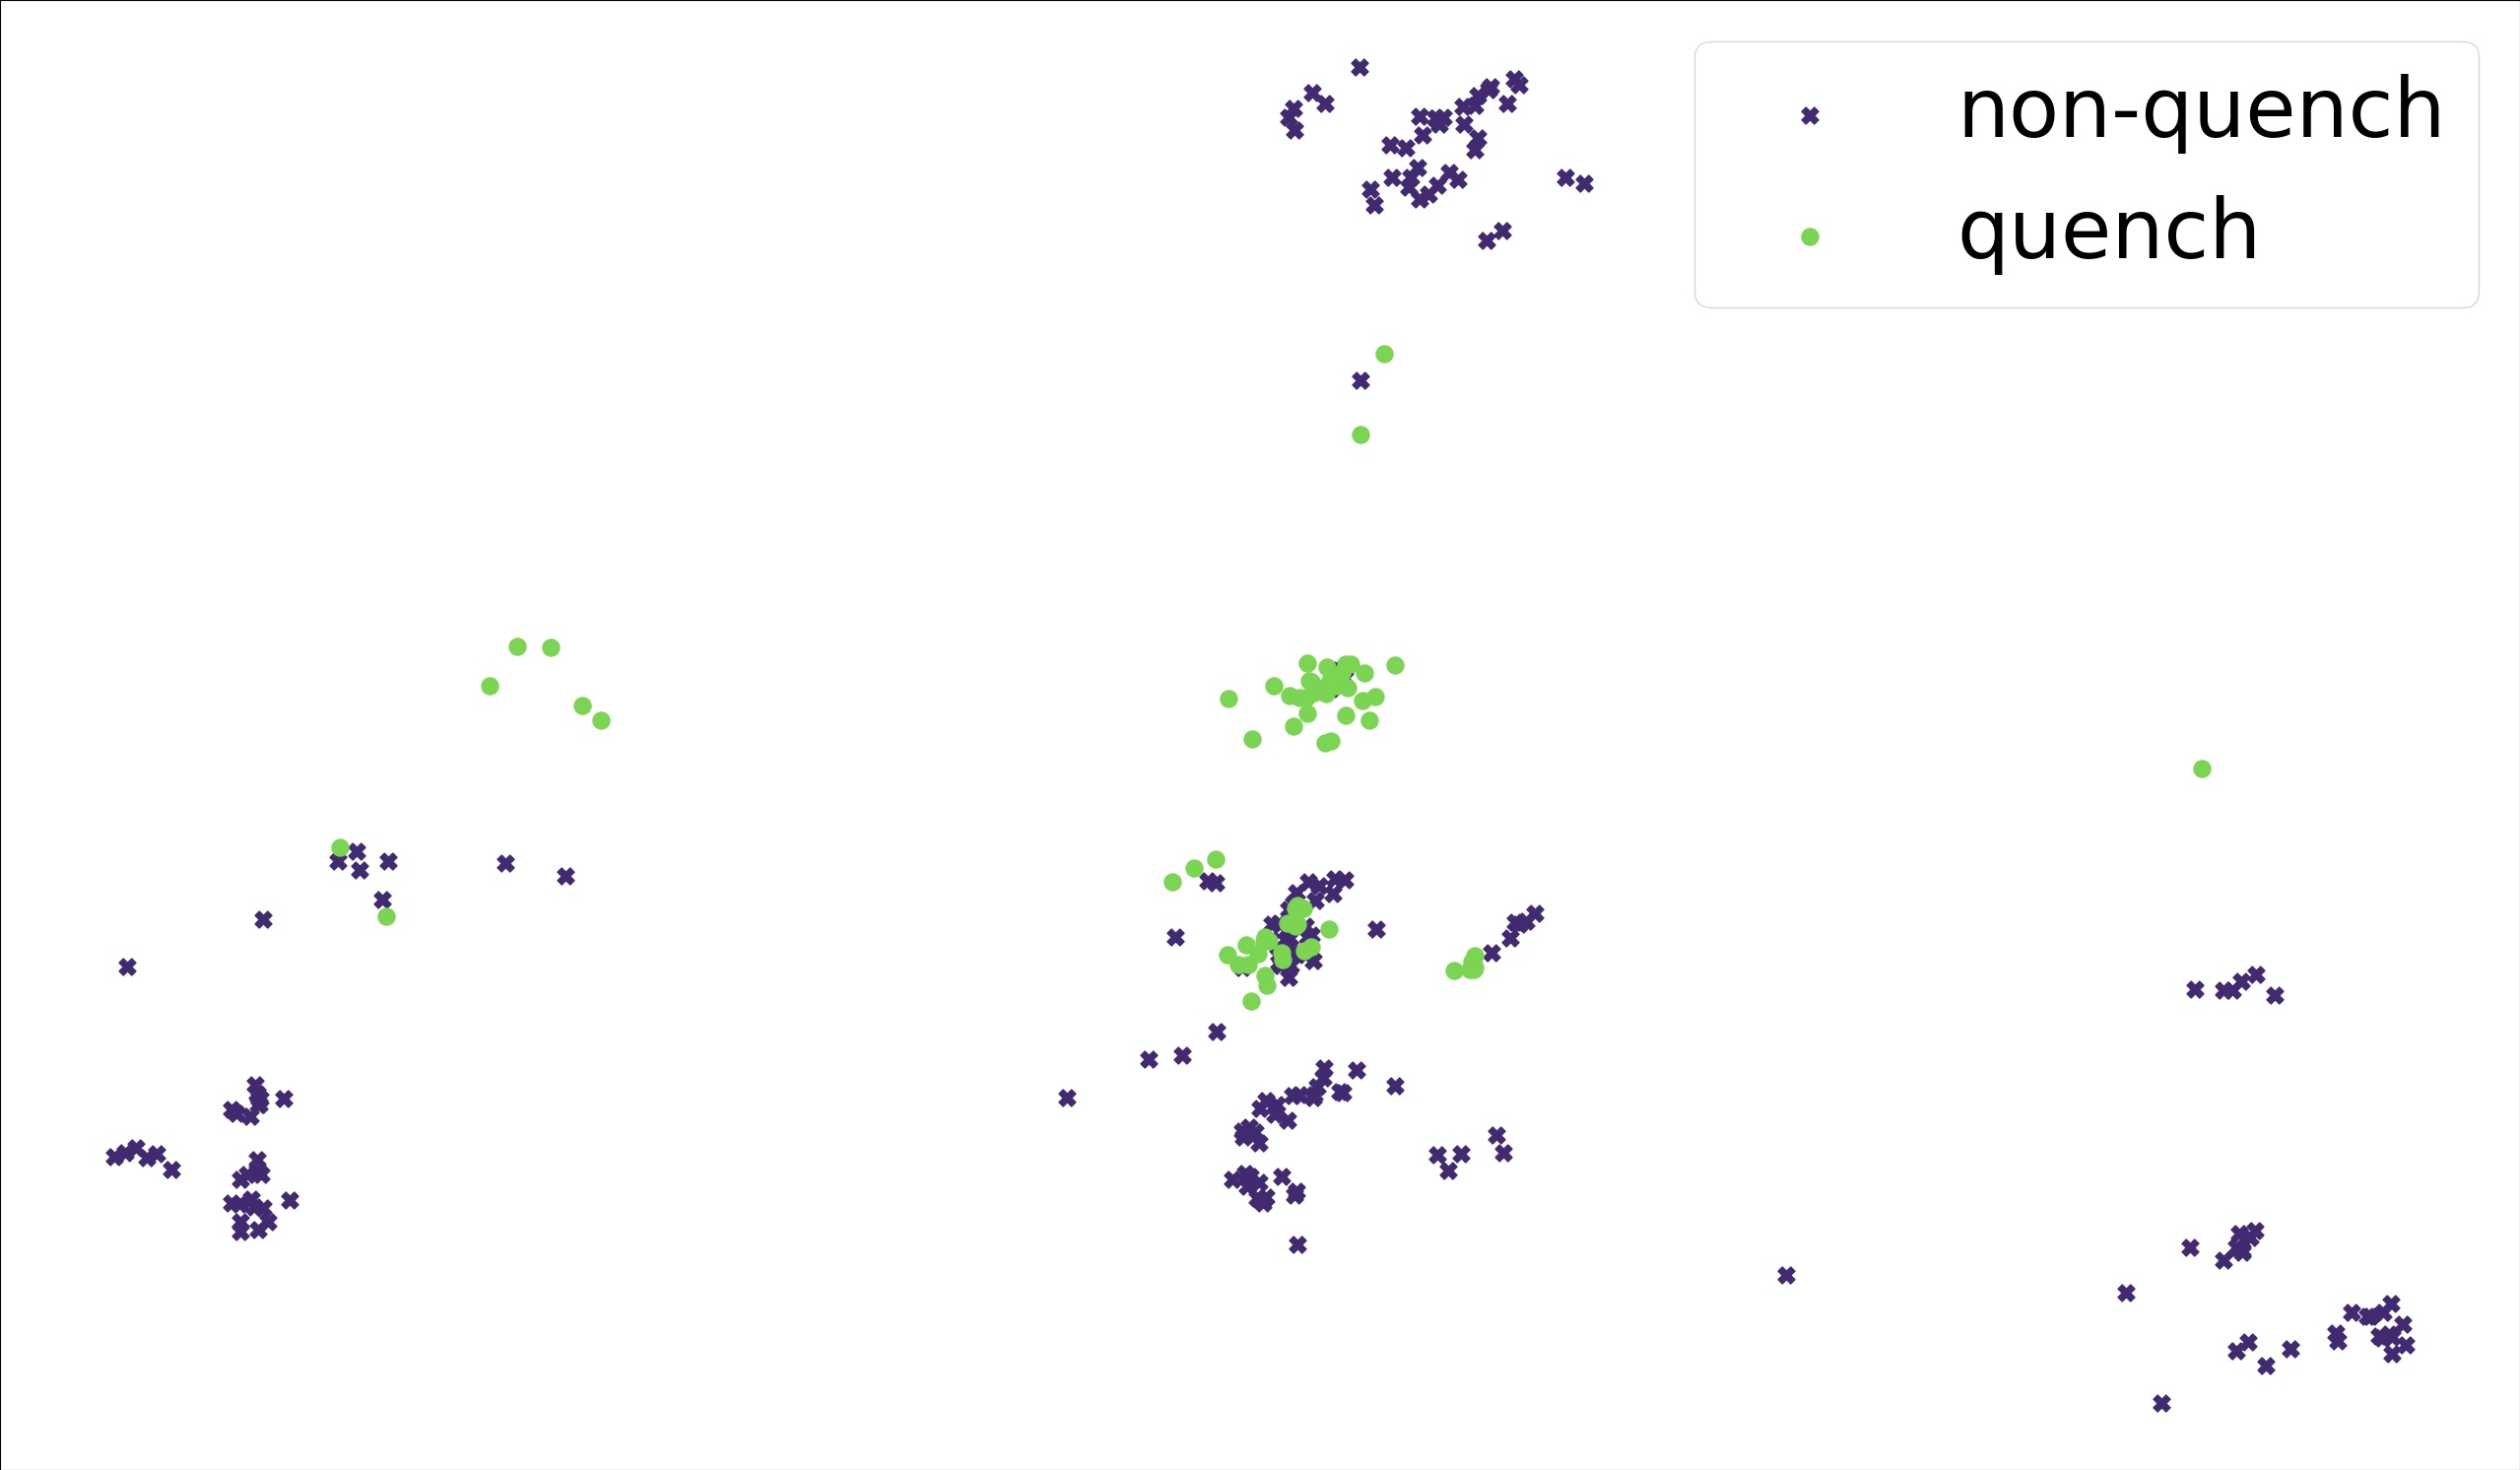
\includegraphics[width=\linewidth]{img/quench_dist_qlp/quenches_coil_3_An.png}
		\subcaption{}
	\end{subfigure}
	\caption{The distribution of the samples in bidimensional space after a round of \pca, for
		the \an\ attribute. The sub-figures contain different views of the same data: (a) differenciates between non-quench and single or multiple quench events, (b) highlights the distribution of quenches for coil $0$, (c) highlights the distribution of quenches for coil $1$, (d) highlights the distribution of quenches for coil $2$ and finally (e) highlights the distribution of quenches for coil $3$.}
	\label{fig:an-coilq-dist}
\end{figure}

\subsubsection{\bn}
In \qrp, \bn\ was the worst attribute we could use, because it contained a very low amounts of
information and samples were distributed very poorly (see \Cref{fig:bn-dist}). We did expect the
same for \qlp, but, as it turns out, \bn\ contains a good amount of information that are
'complementary' to the ones contained in \an.

\Cref{fig:bn-lcorr-qlp} highlights the correlation between \bn\ harmonics and the label associated
to each coil. The attribute, similarly to \an, sees a pattern of strong correlations between its
harmonics and coils $1$ and $3$. Since the pattern of sub-figures (b) and (d) is very similar to the
one shown in sub-figures (a) and (c) of \Cref{fig:an-lcorr-qlp}, we were taken to similar
conclusions.
\begin{figure}[!ht]
	% Font size = 70
	\centering
	\begin{subfigure}{0.49\linewidth}
		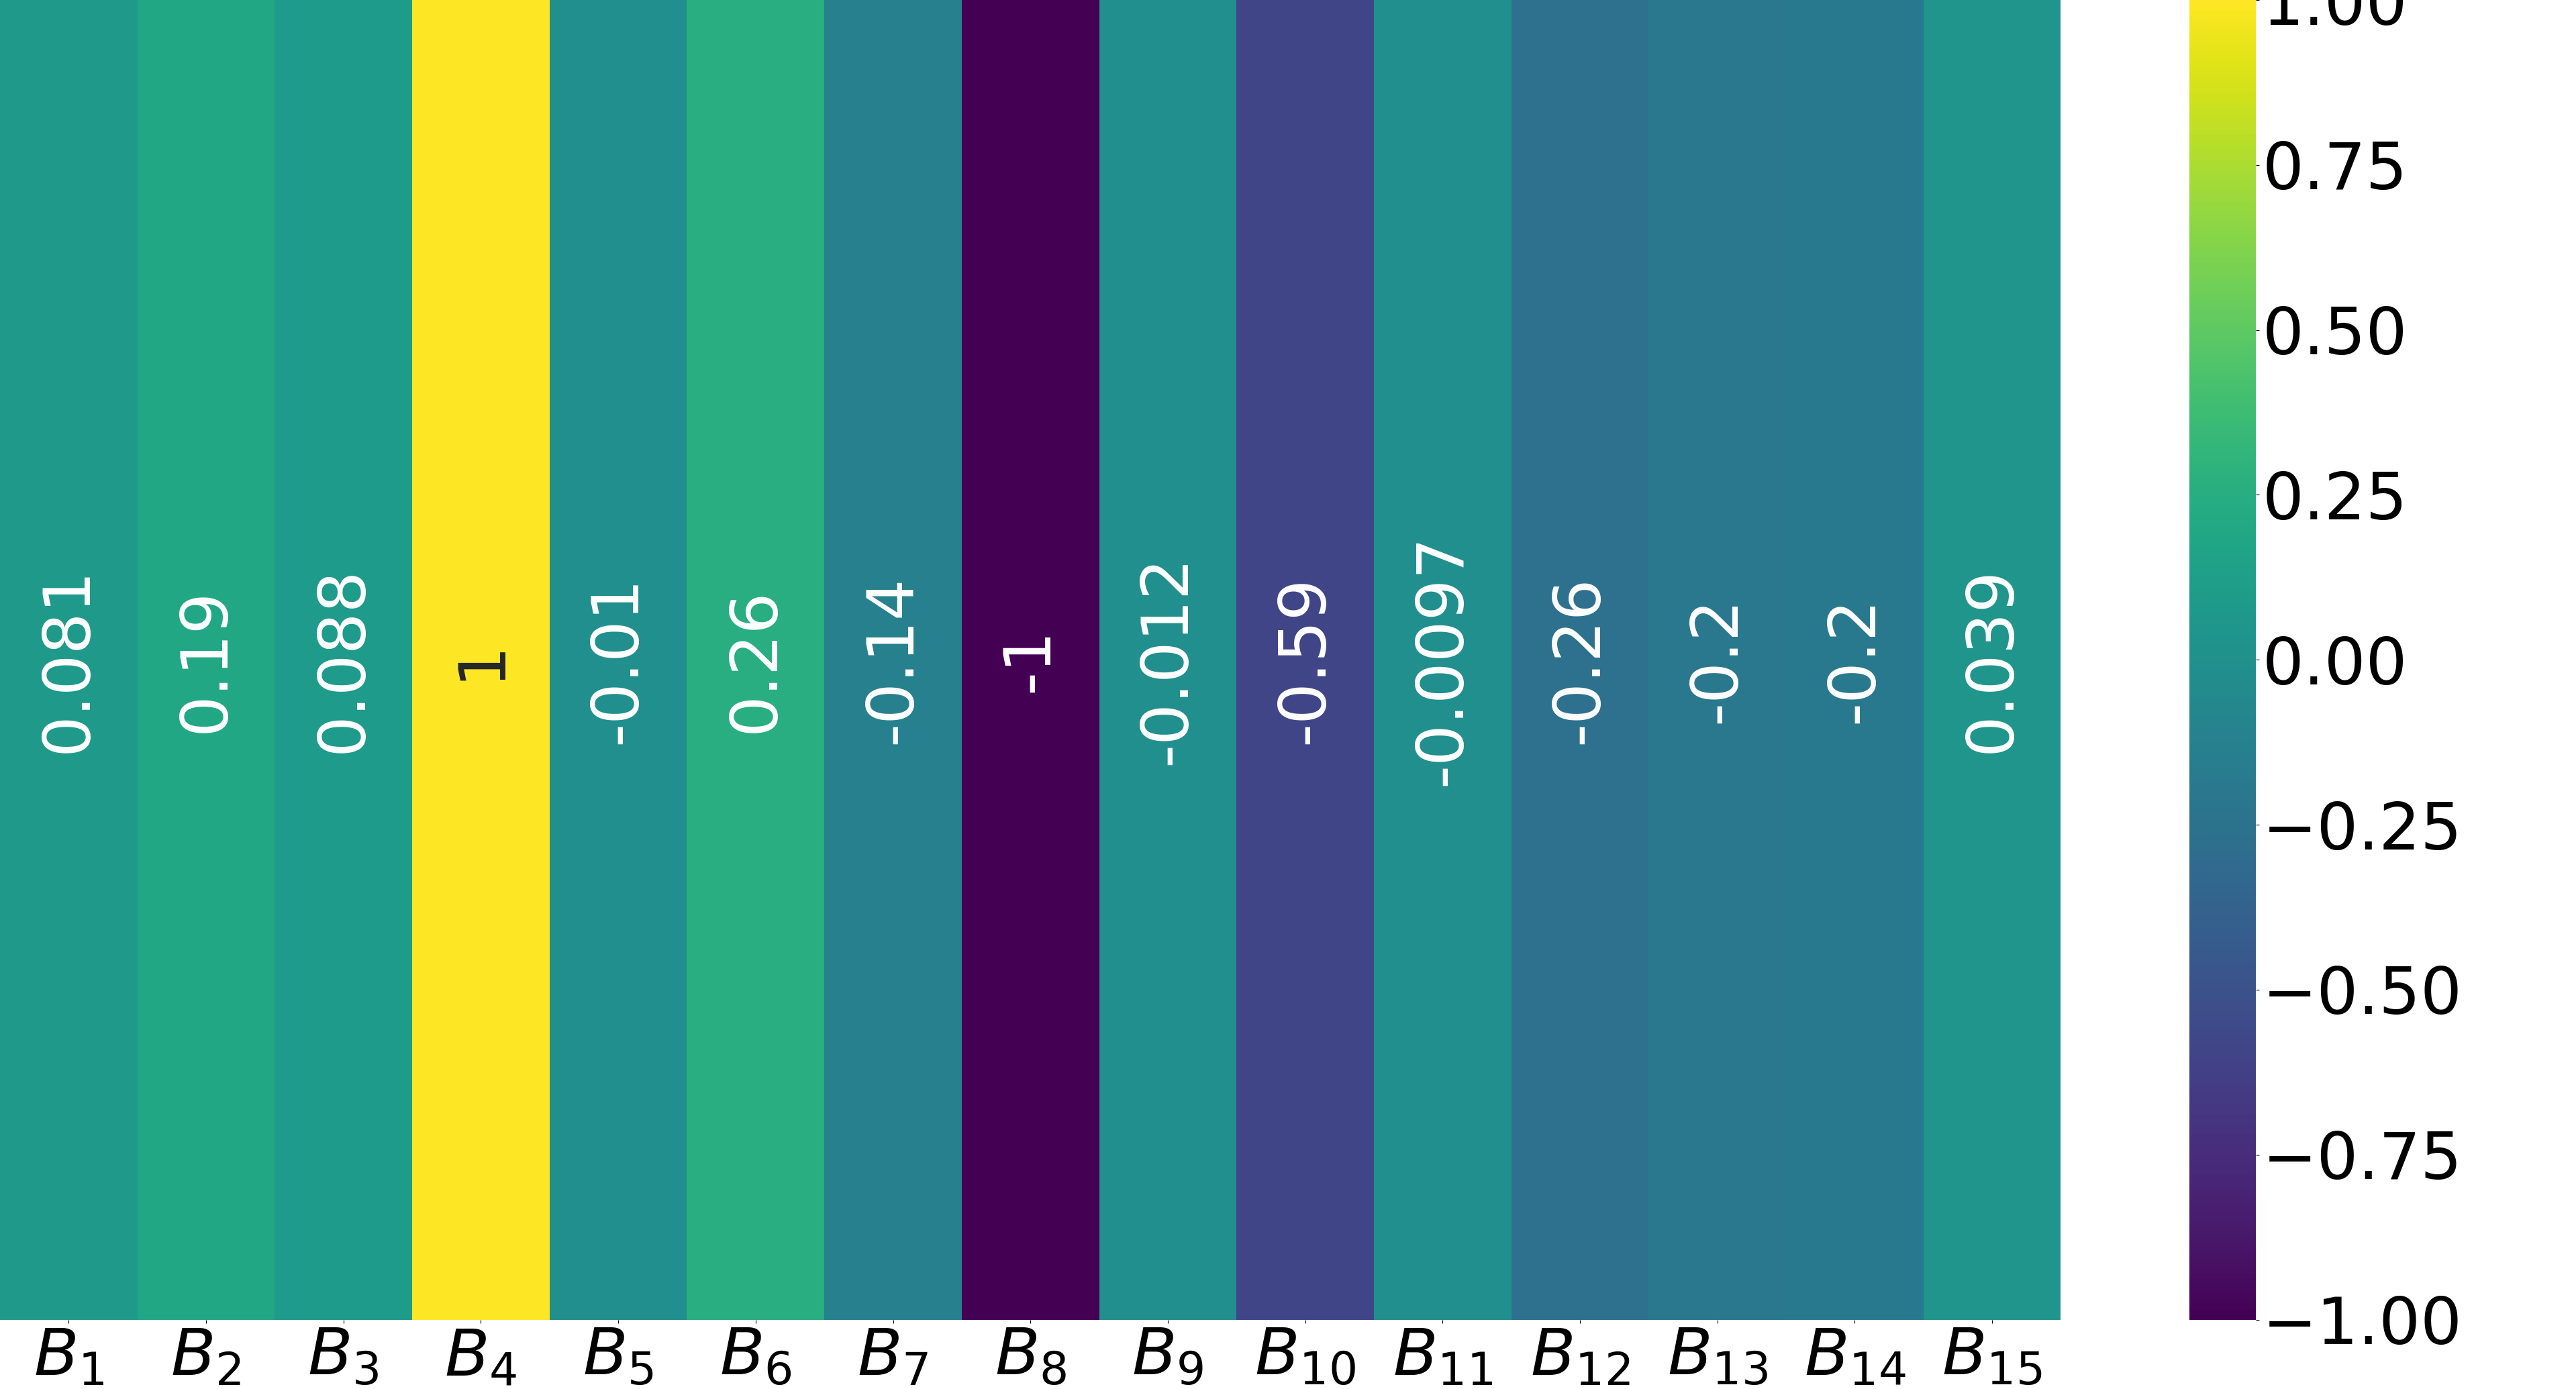
\includegraphics[width=\linewidth]{img/qlp_corr/Bn_coil0.png}
		\subcaption{Correlation with coil $0$}
	\end{subfigure}
	\begin{subfigure}{0.49\linewidth}
		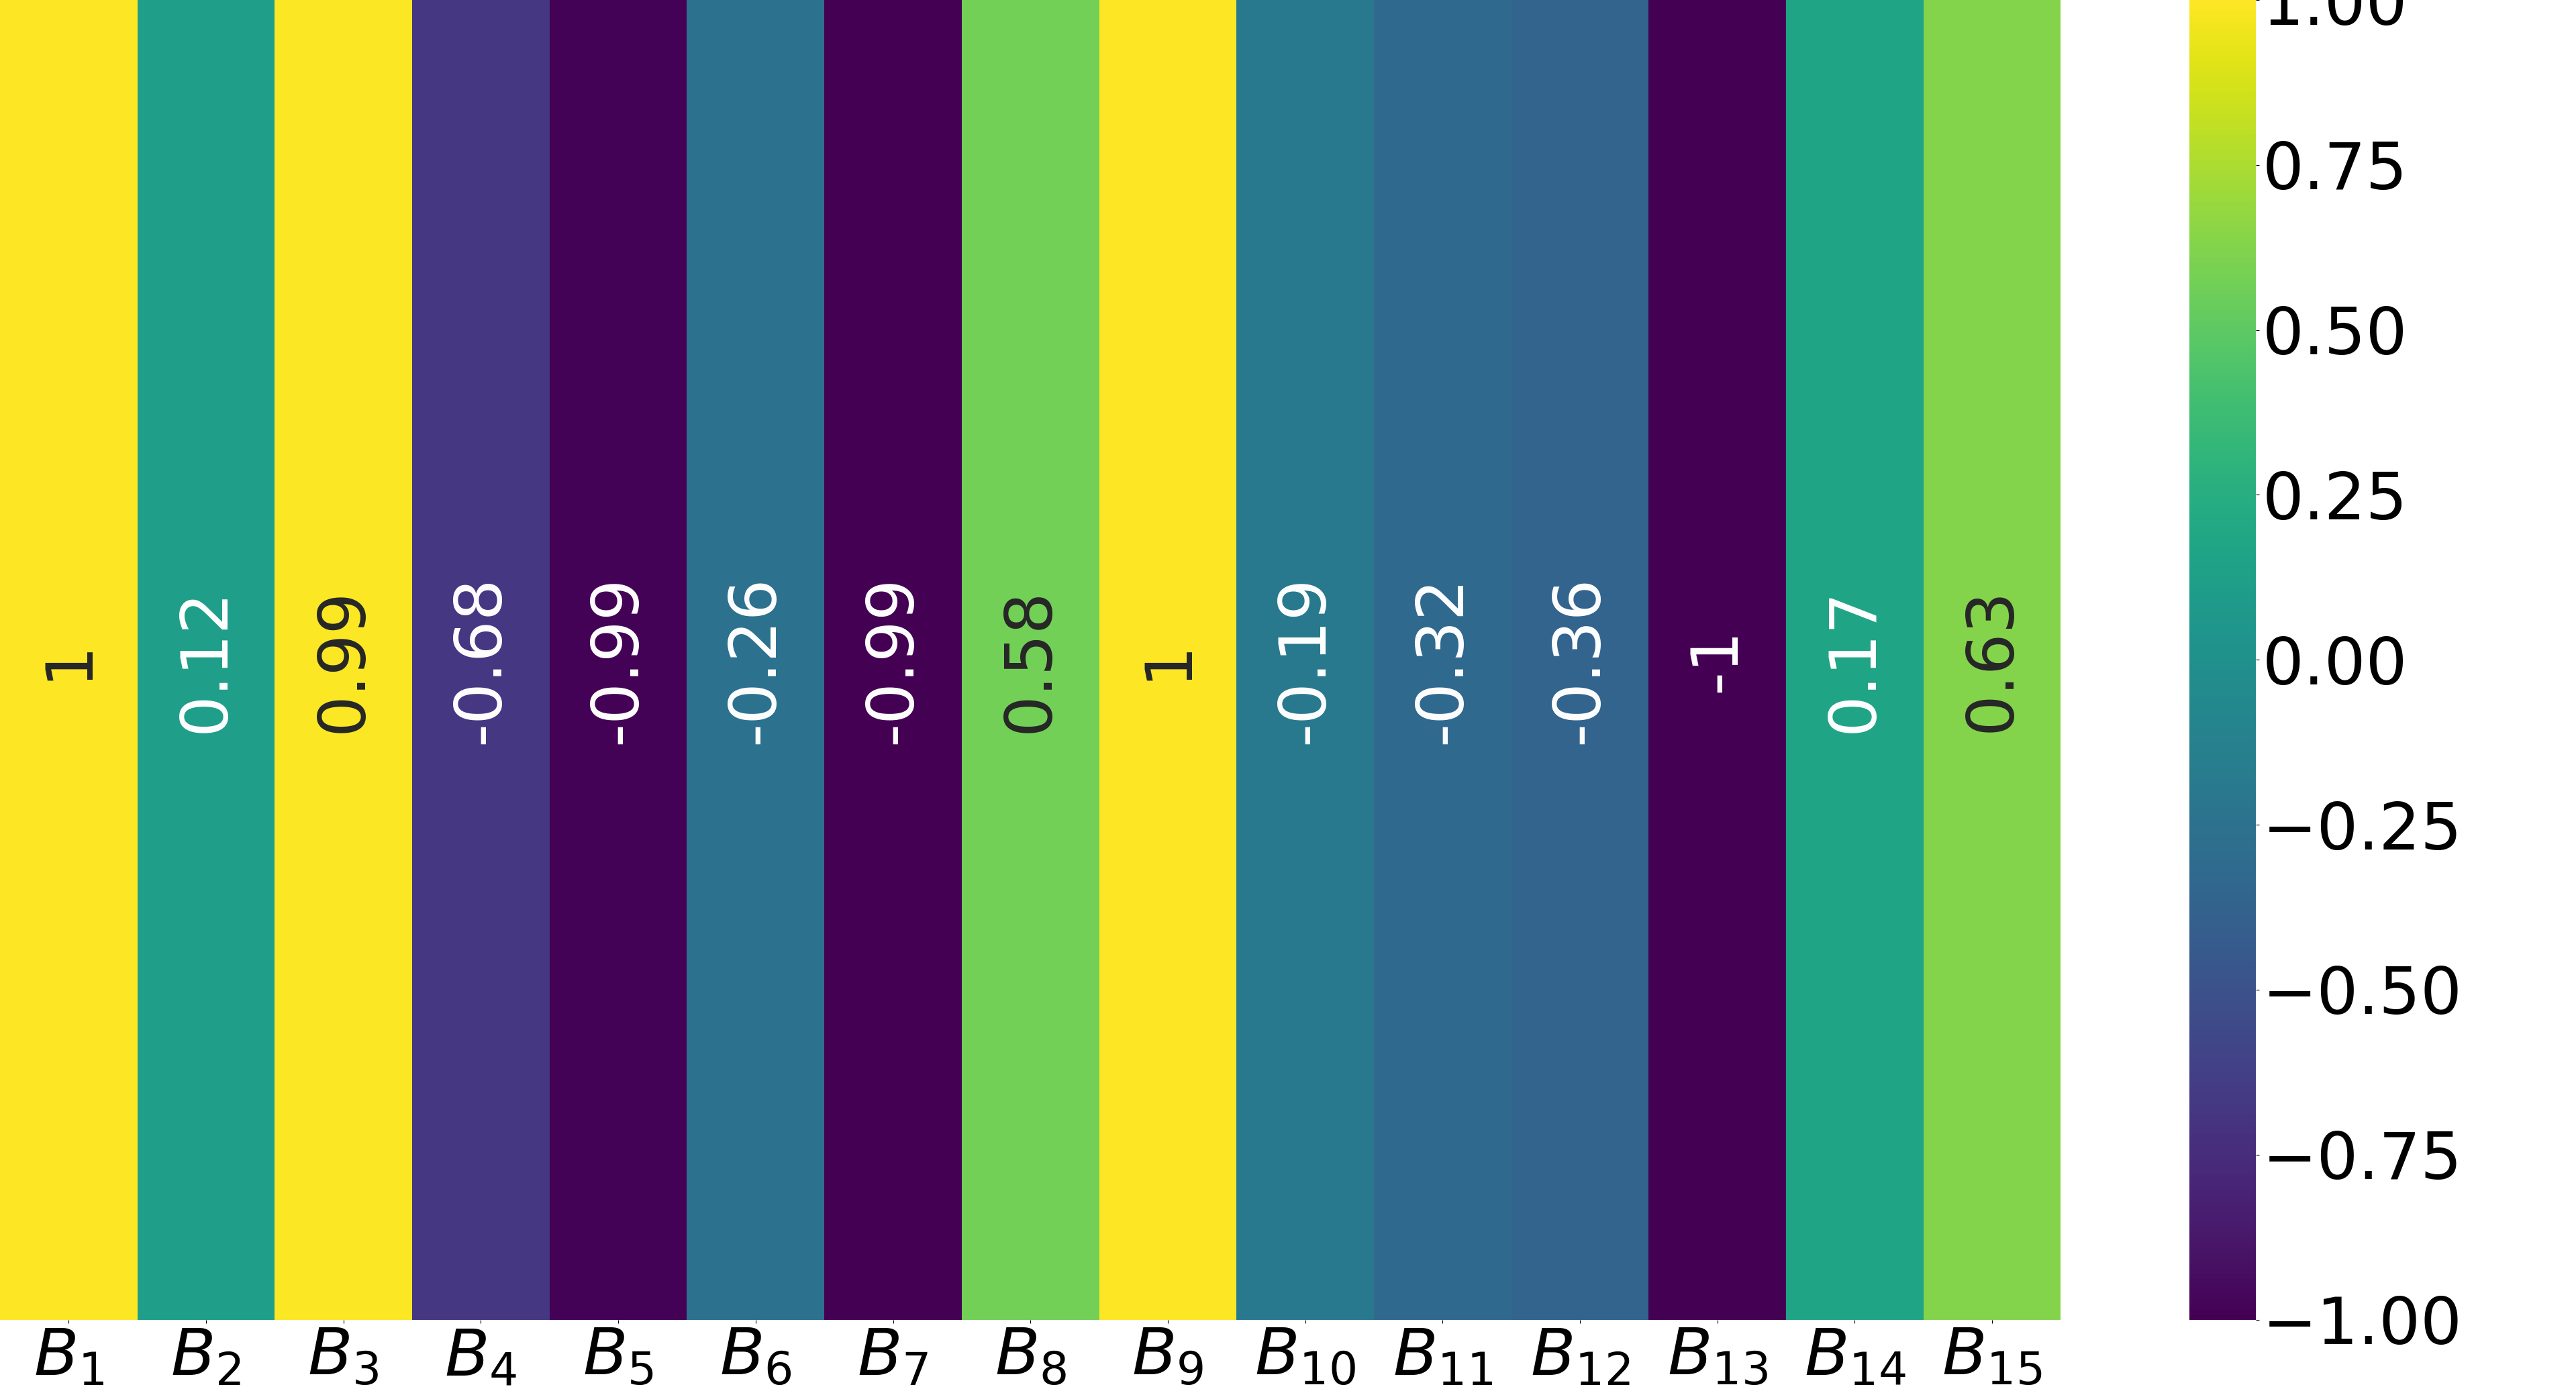
\includegraphics[width=\linewidth]{img/qlp_corr/Bn_coil1.png}
		\subcaption{Correlation with coil $1$}
	\end{subfigure}
	\begin{subfigure}{0.49\linewidth}
		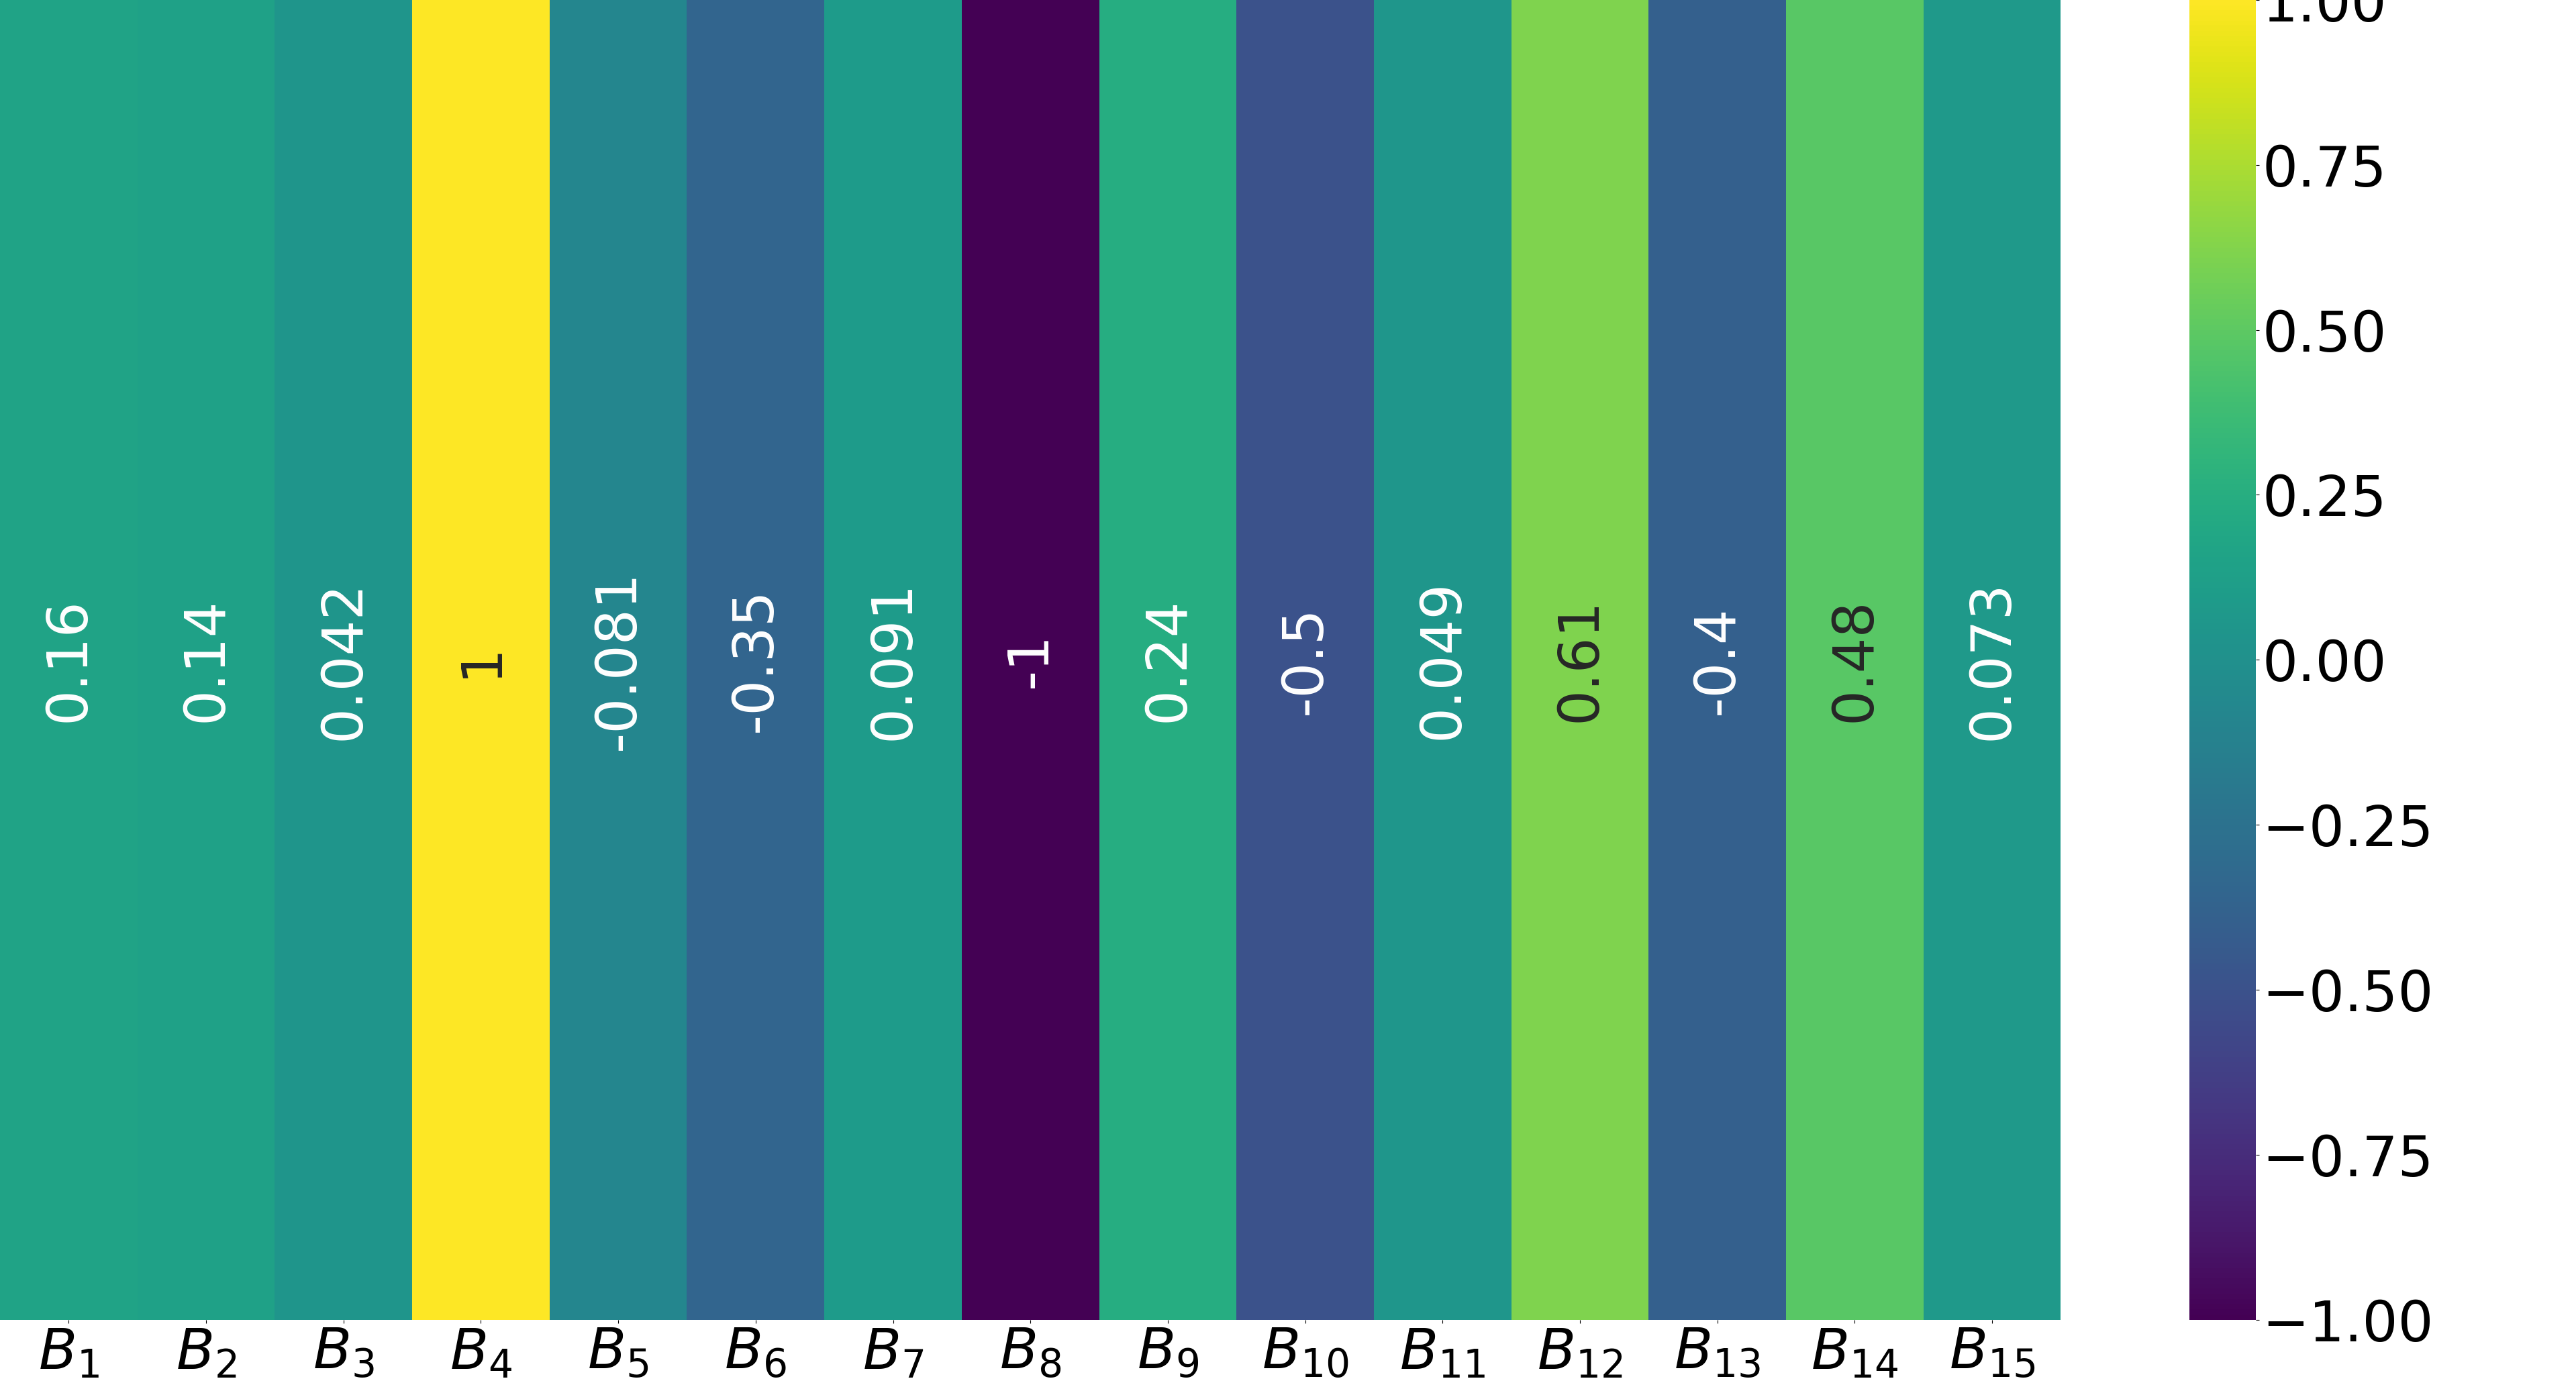
\includegraphics[width=\linewidth]{img/qlp_corr/Bn_coil2.png}
		\subcaption{Correlation with coil $2$}
	\end{subfigure}
	\begin{subfigure}{0.49\linewidth}
		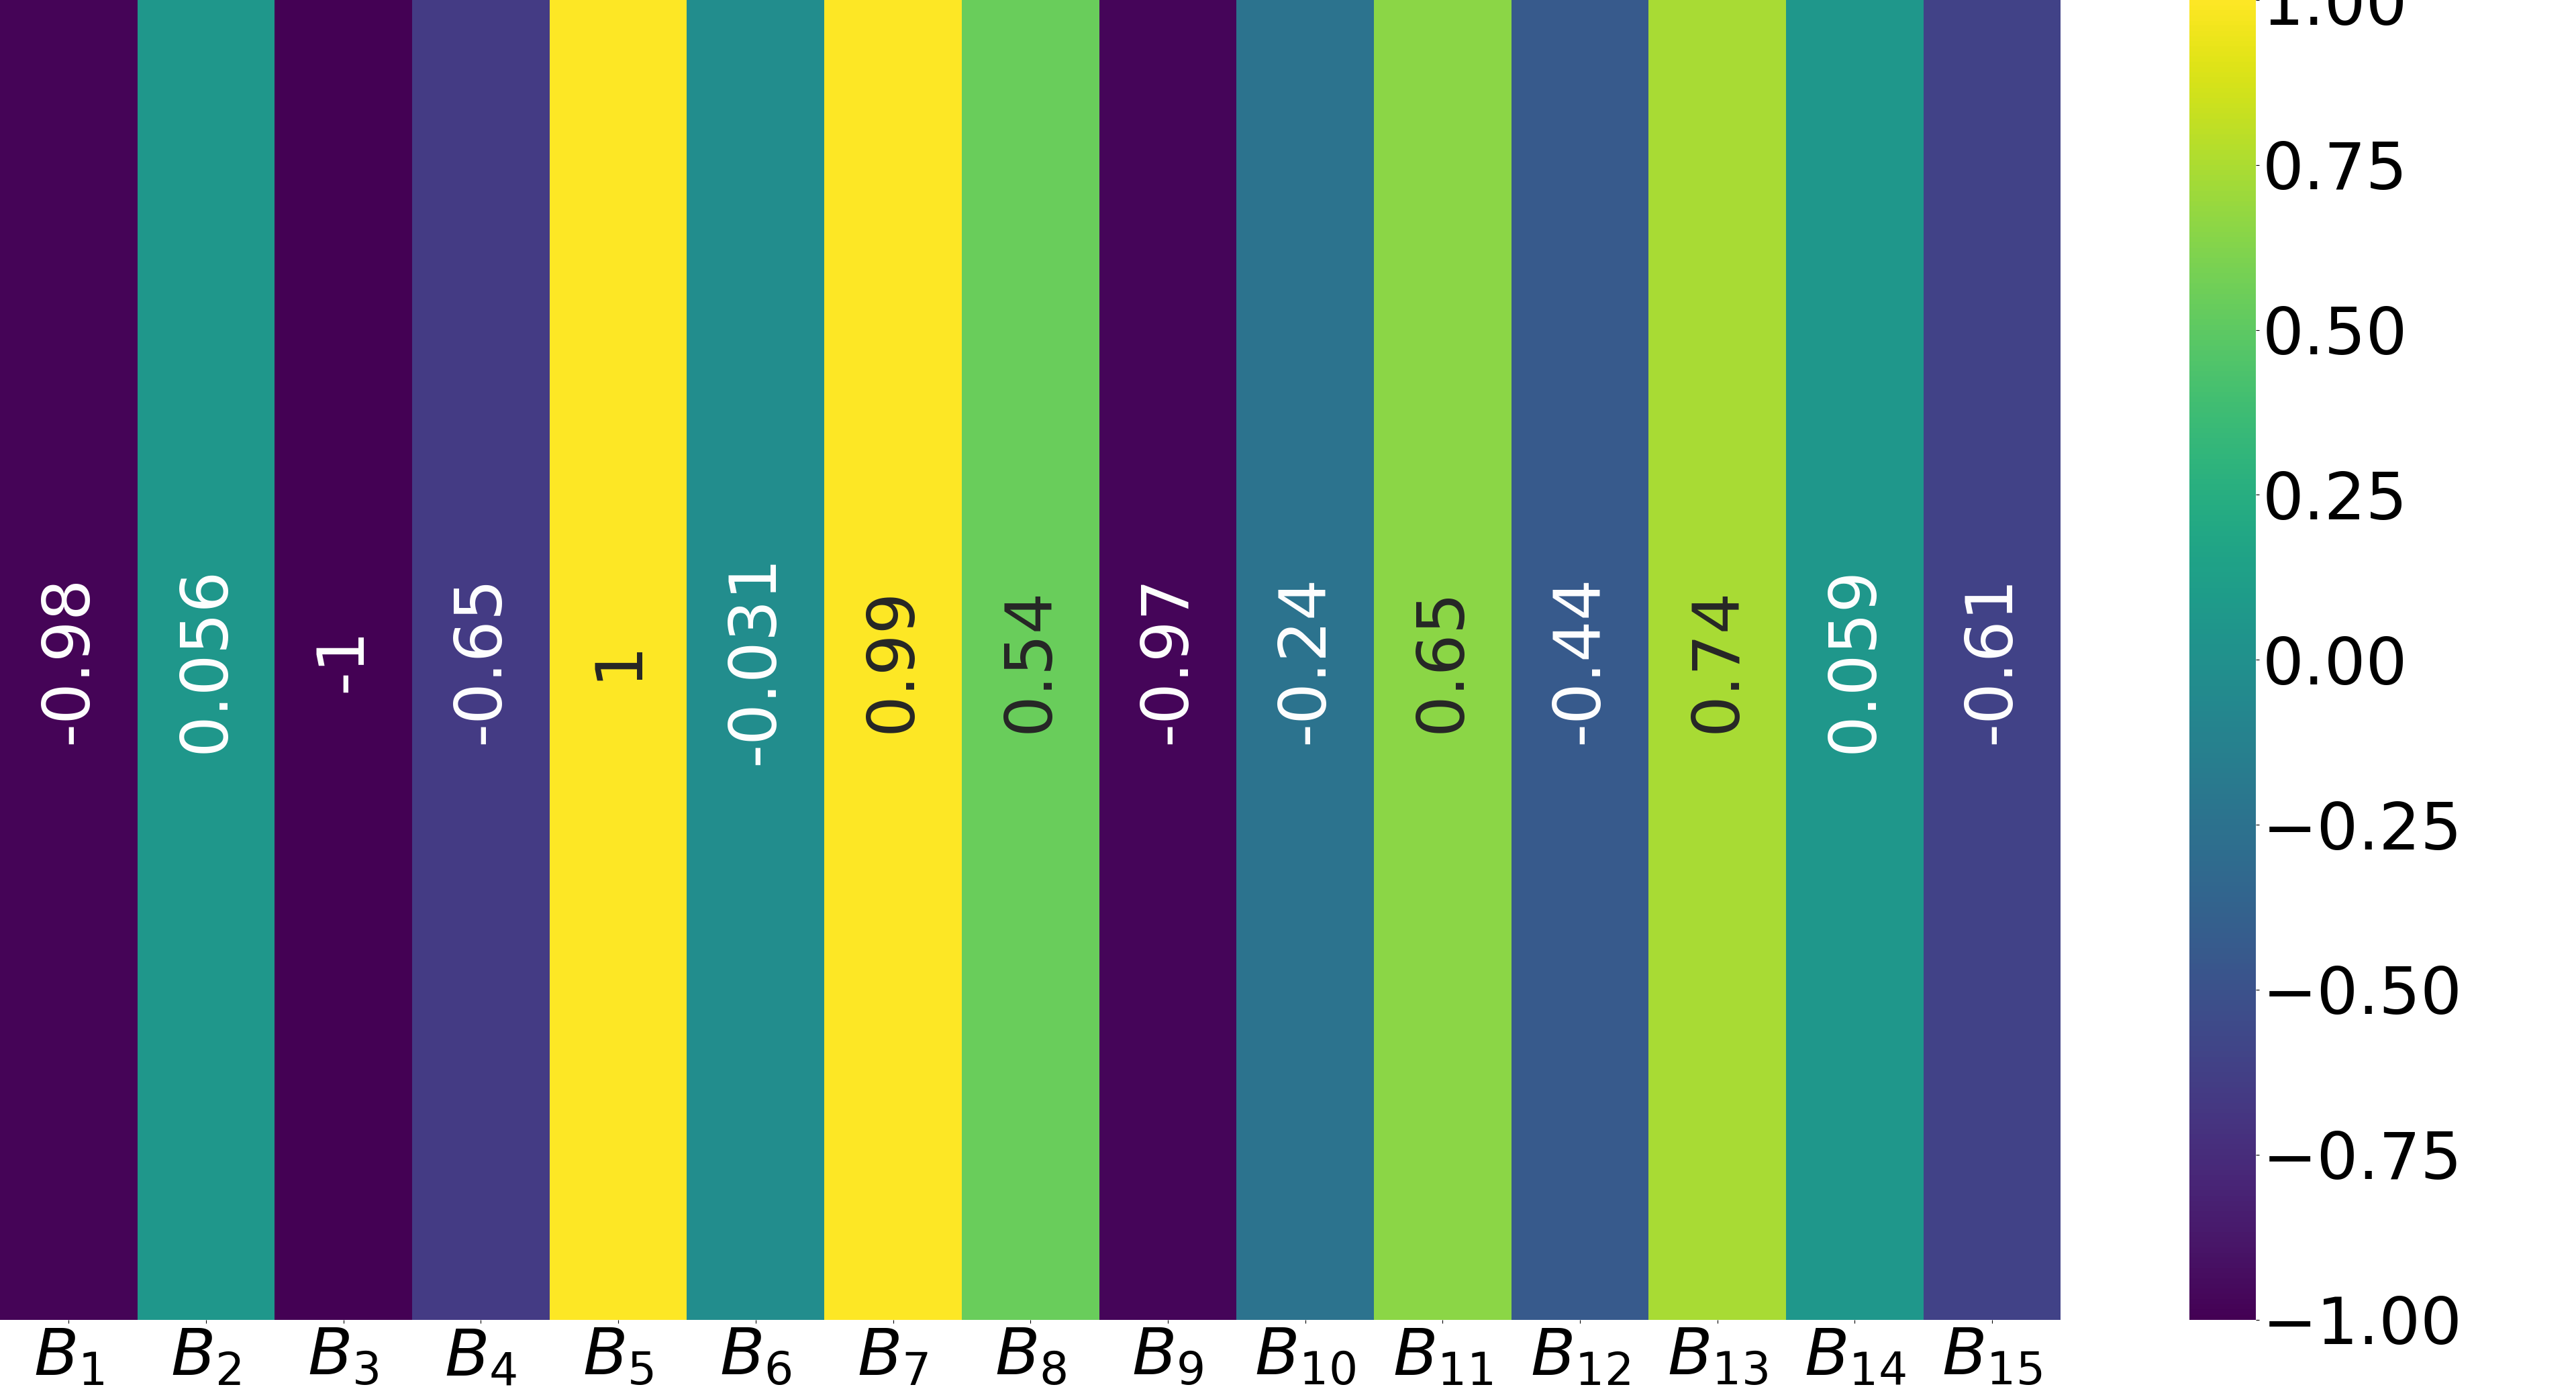
\includegraphics[width=\linewidth]{img/qlp_corr/Bn_coil3.png}
		\subcaption{Correlation with coil $3$}
	\end{subfigure}
	\caption{Correlation between the harmonics of the \bn\ attribute and the labels for \qlp.}
	\label{fig:bn-lcorr-qlp}
\end{figure}

In \Cref{fig:bn-coilq-dist} we propose different visualizations of the samples contained in \bn\
after a round of \pca. Independently of the sub-figure we consider it's clear that the level of
homogeneity of the samples belonging to the central cluster is very high. While this, alone, cannot
induce us to think that the performance for models based on \bn\ is going to be bad, we are drawn to
consider the possibility that \bn\ might not be a good enough attribute if taken on its own.

\begin{figure}[!h]
	% Font size = 70
	\centering
	\begin{subfigure}{\linewidth}
		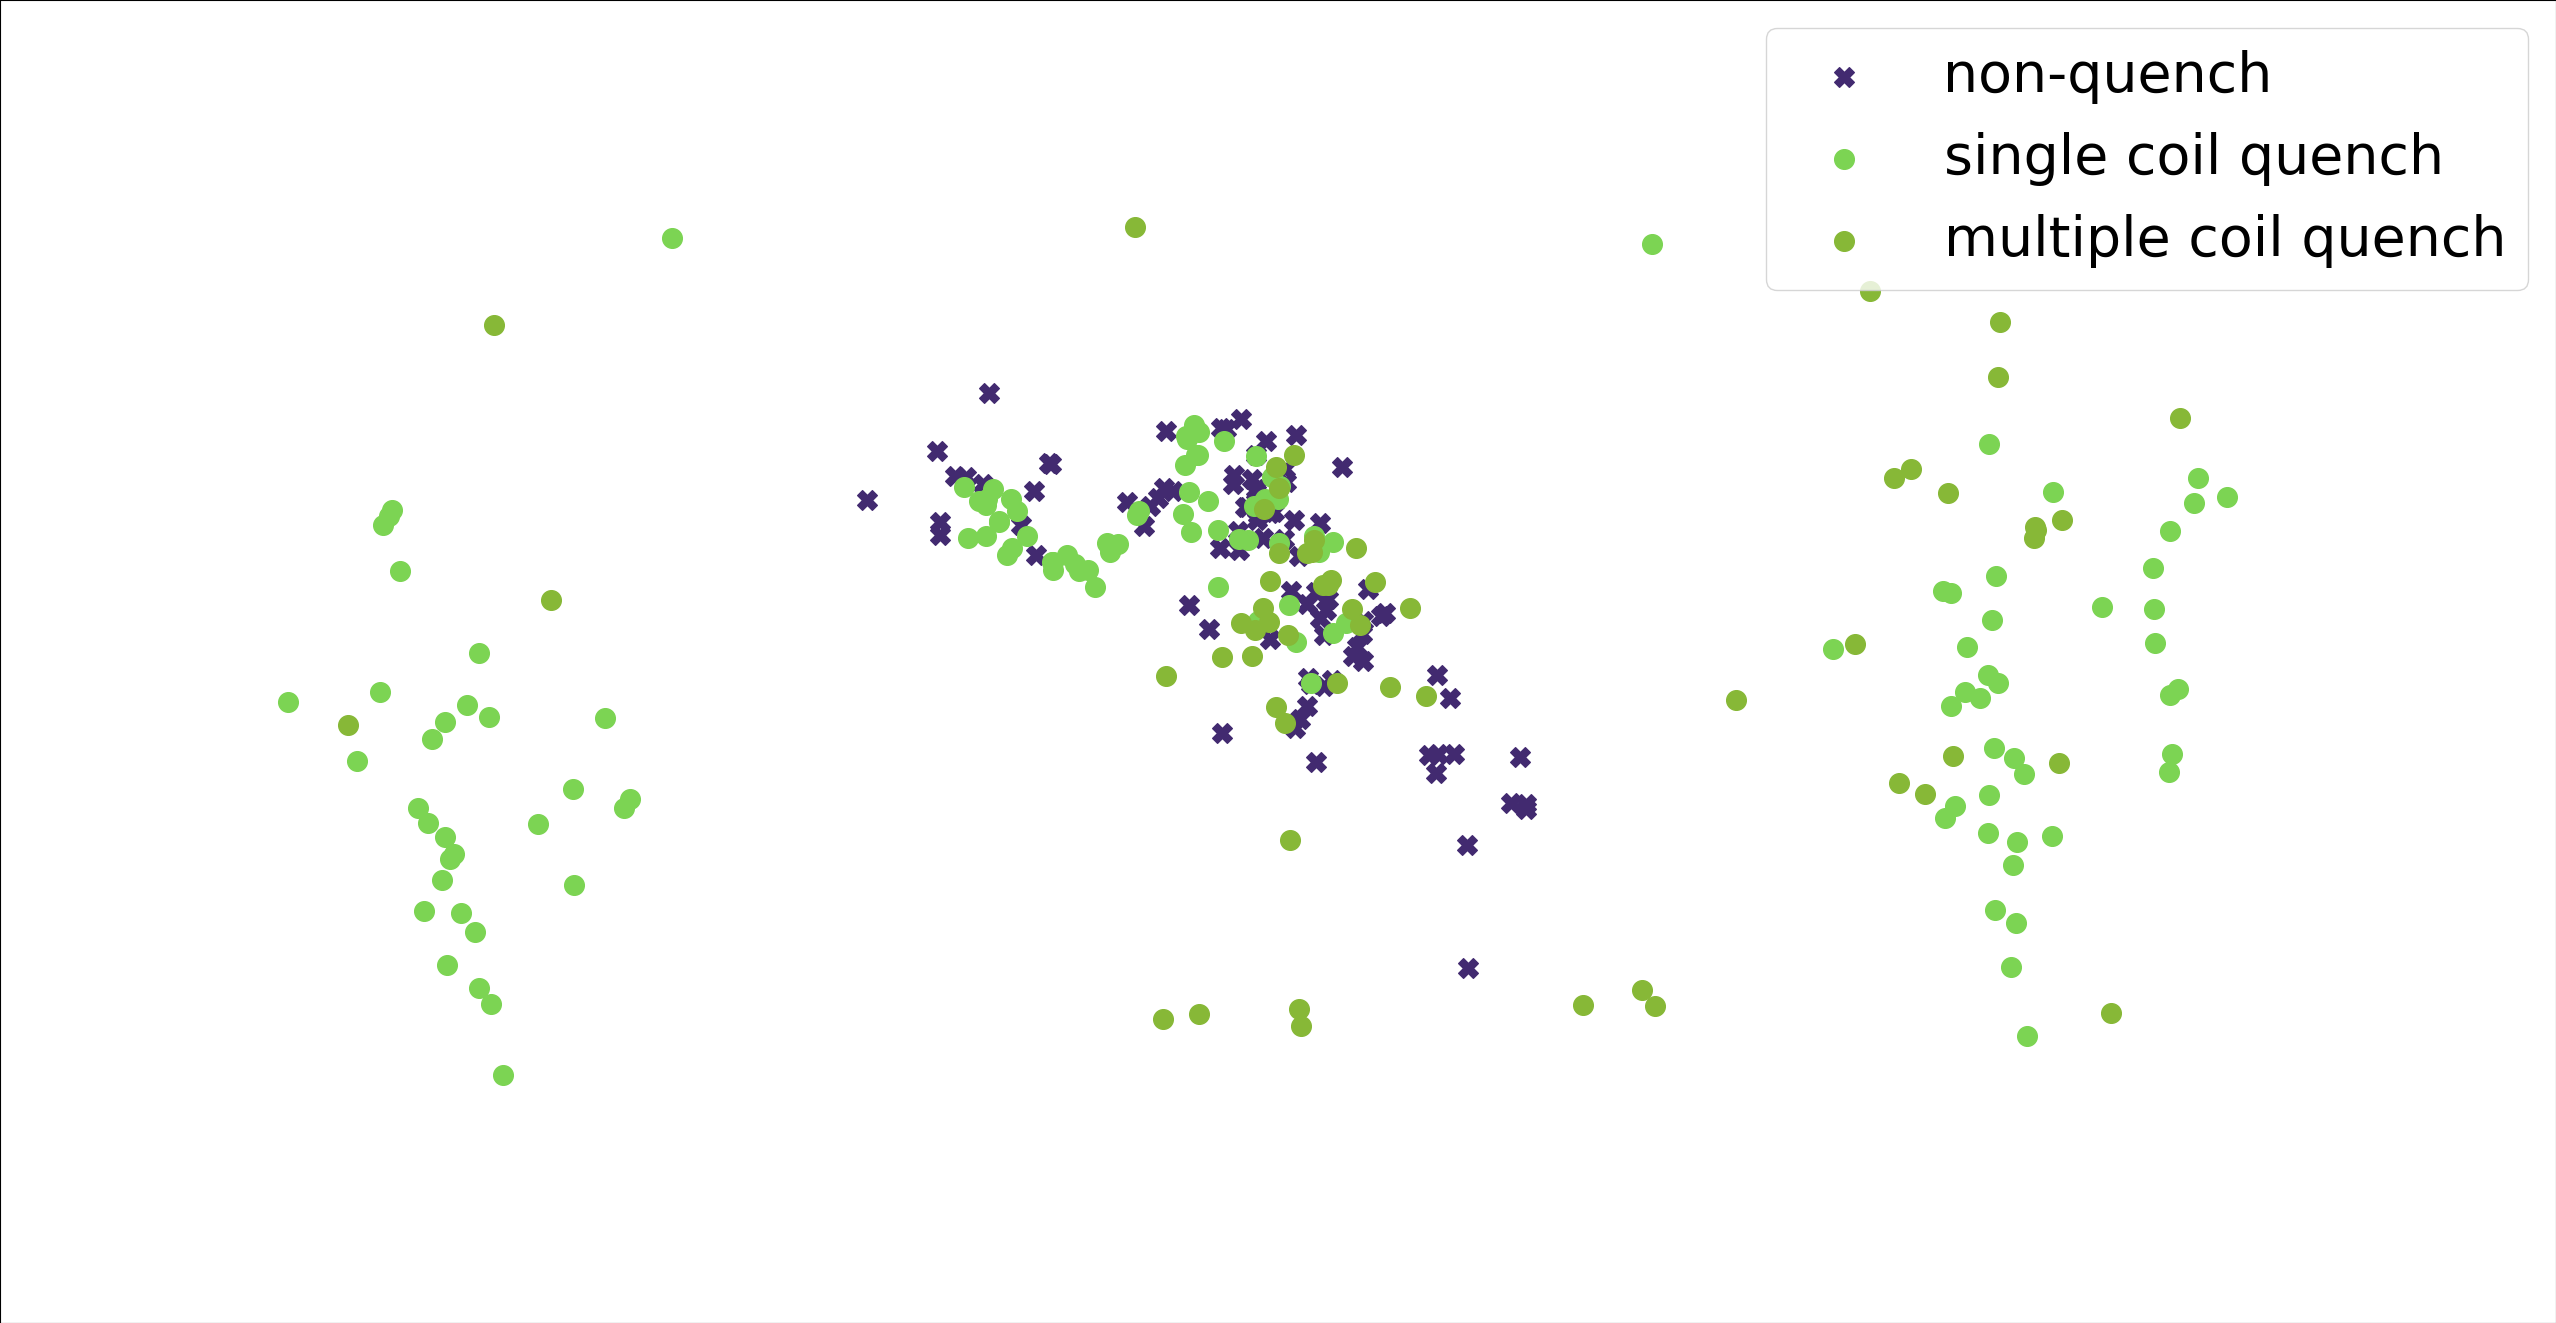
\includegraphics[width=\linewidth]{img/quench_dist_qlp/single_vs_multiple_Bn.png}
		\subcaption{}
	\end{subfigure}
	\begin{subfigure}{0.49\linewidth}
		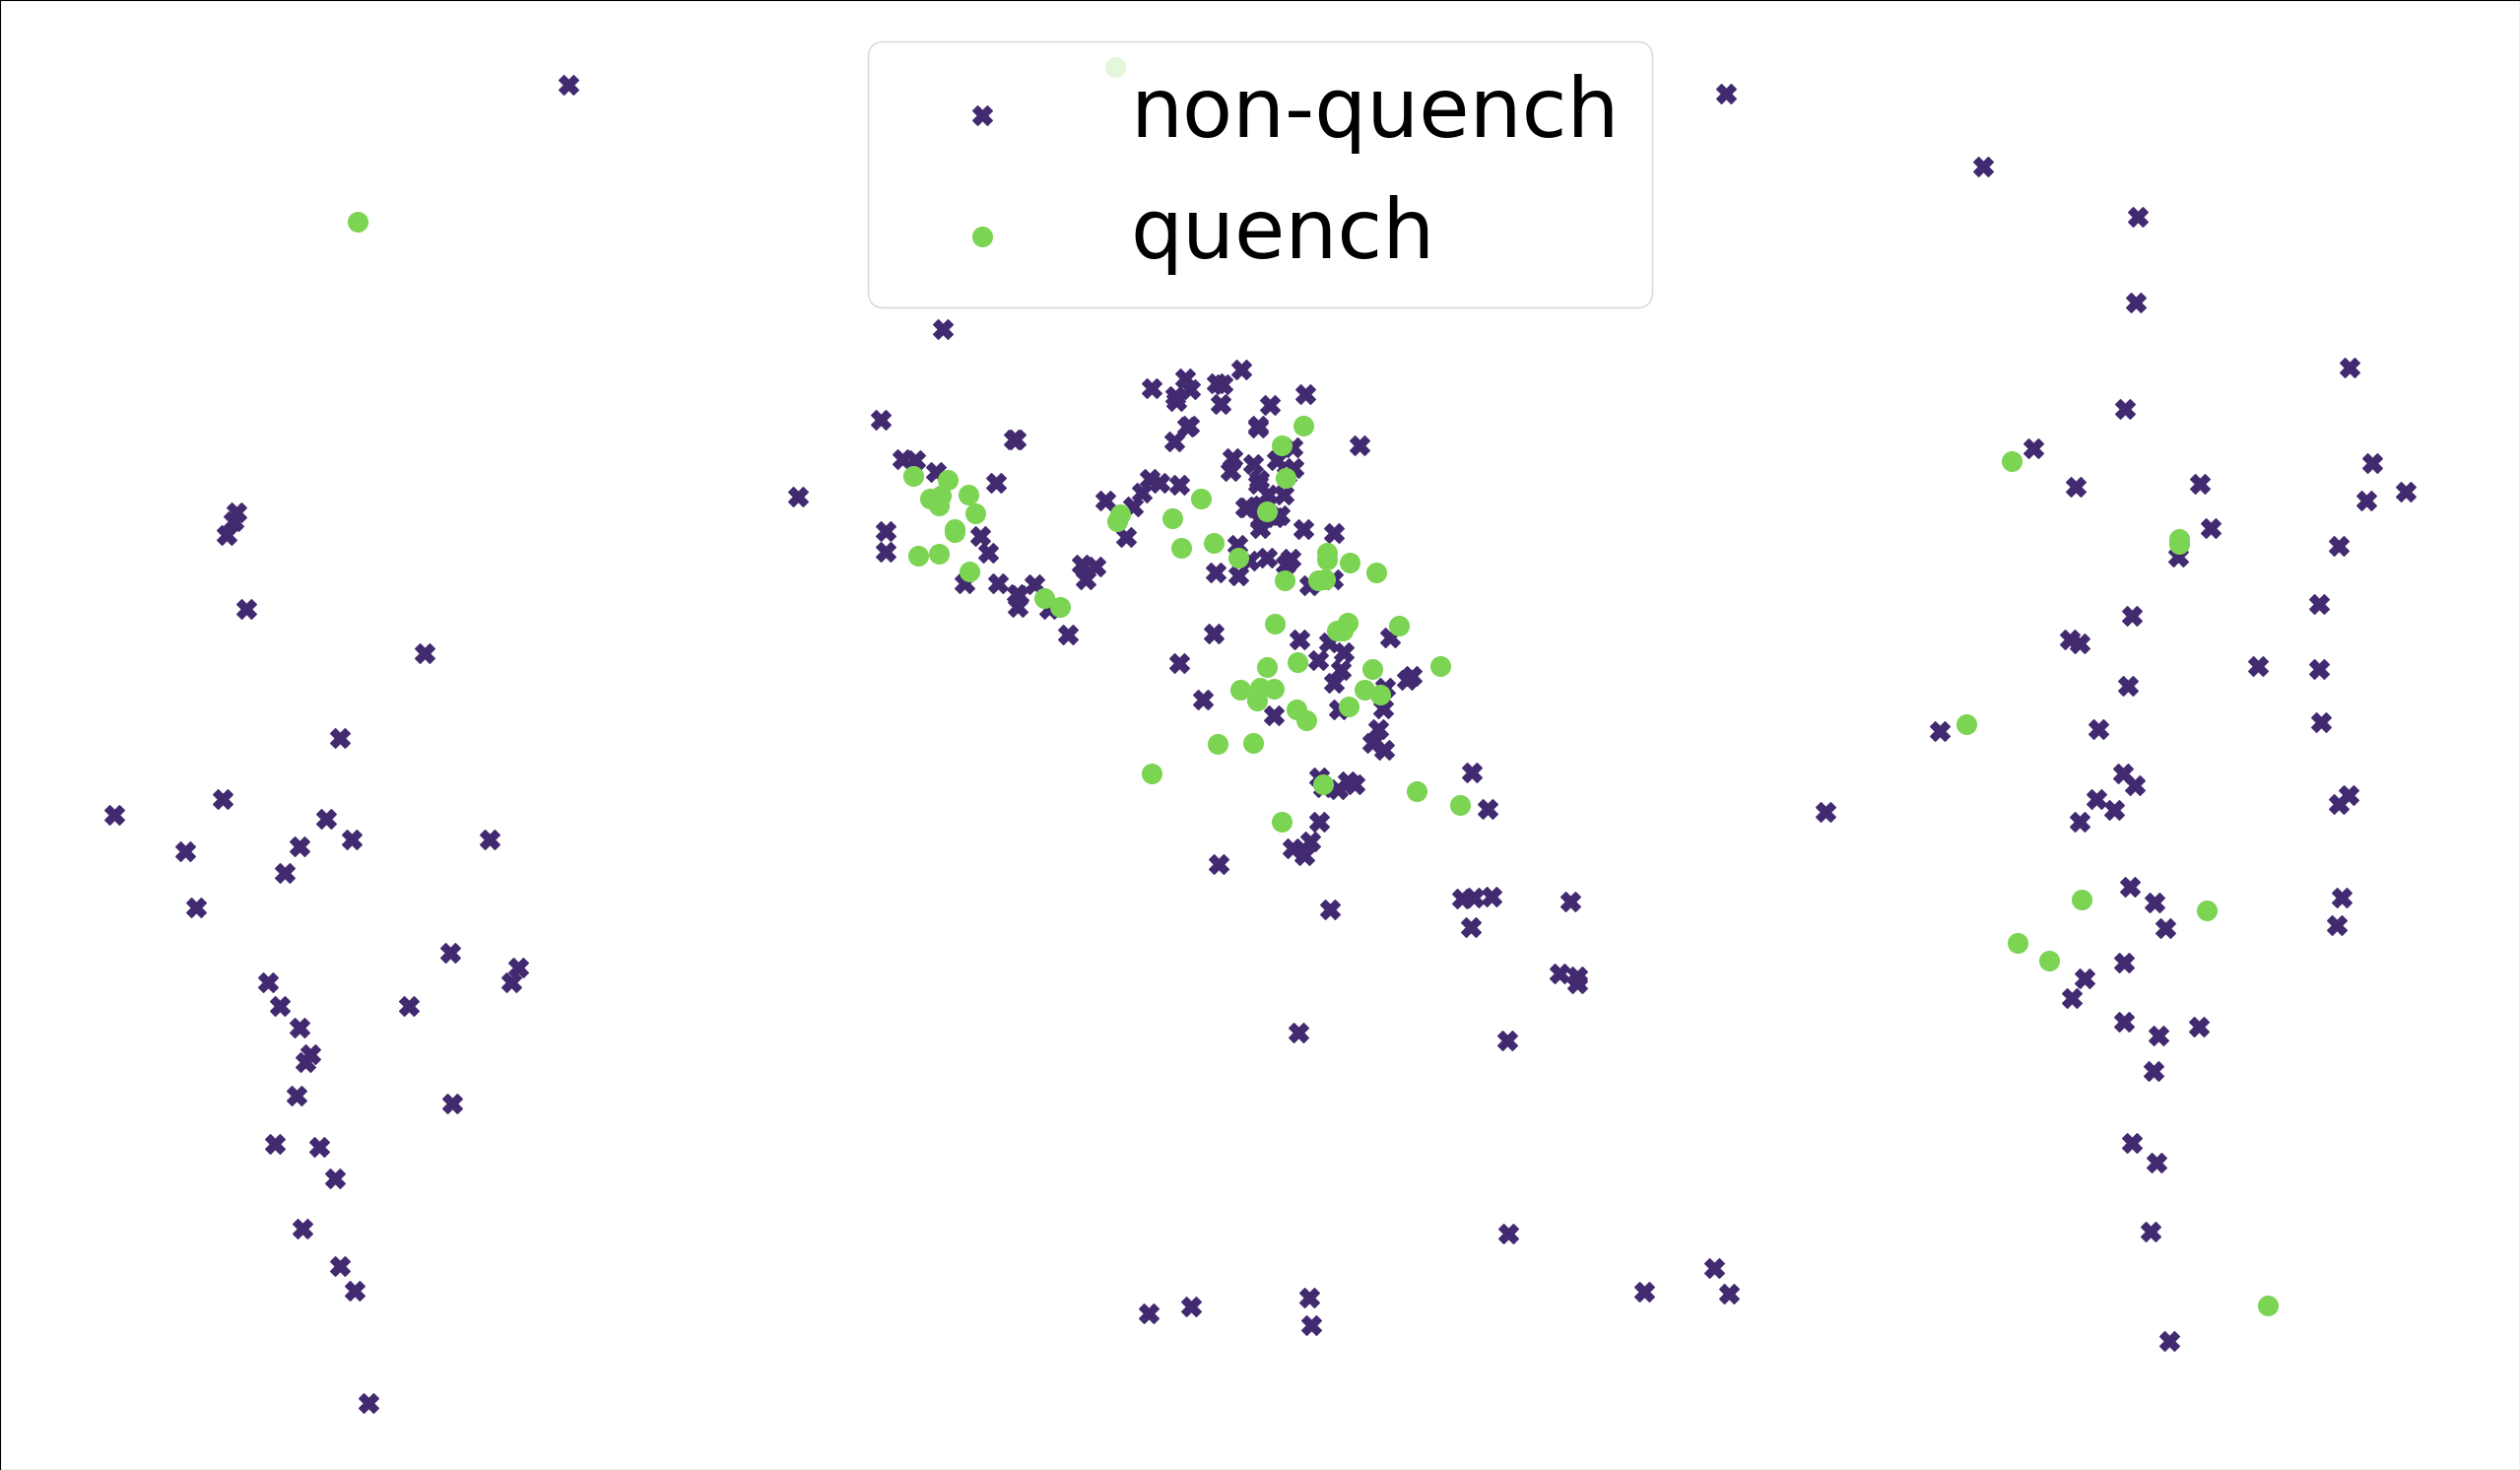
\includegraphics[width=\linewidth]{img/quench_dist_qlp/quenches_coil_0_Bn.png}
		\subcaption{}
	\end{subfigure}
	\begin{subfigure}{0.49\linewidth}
		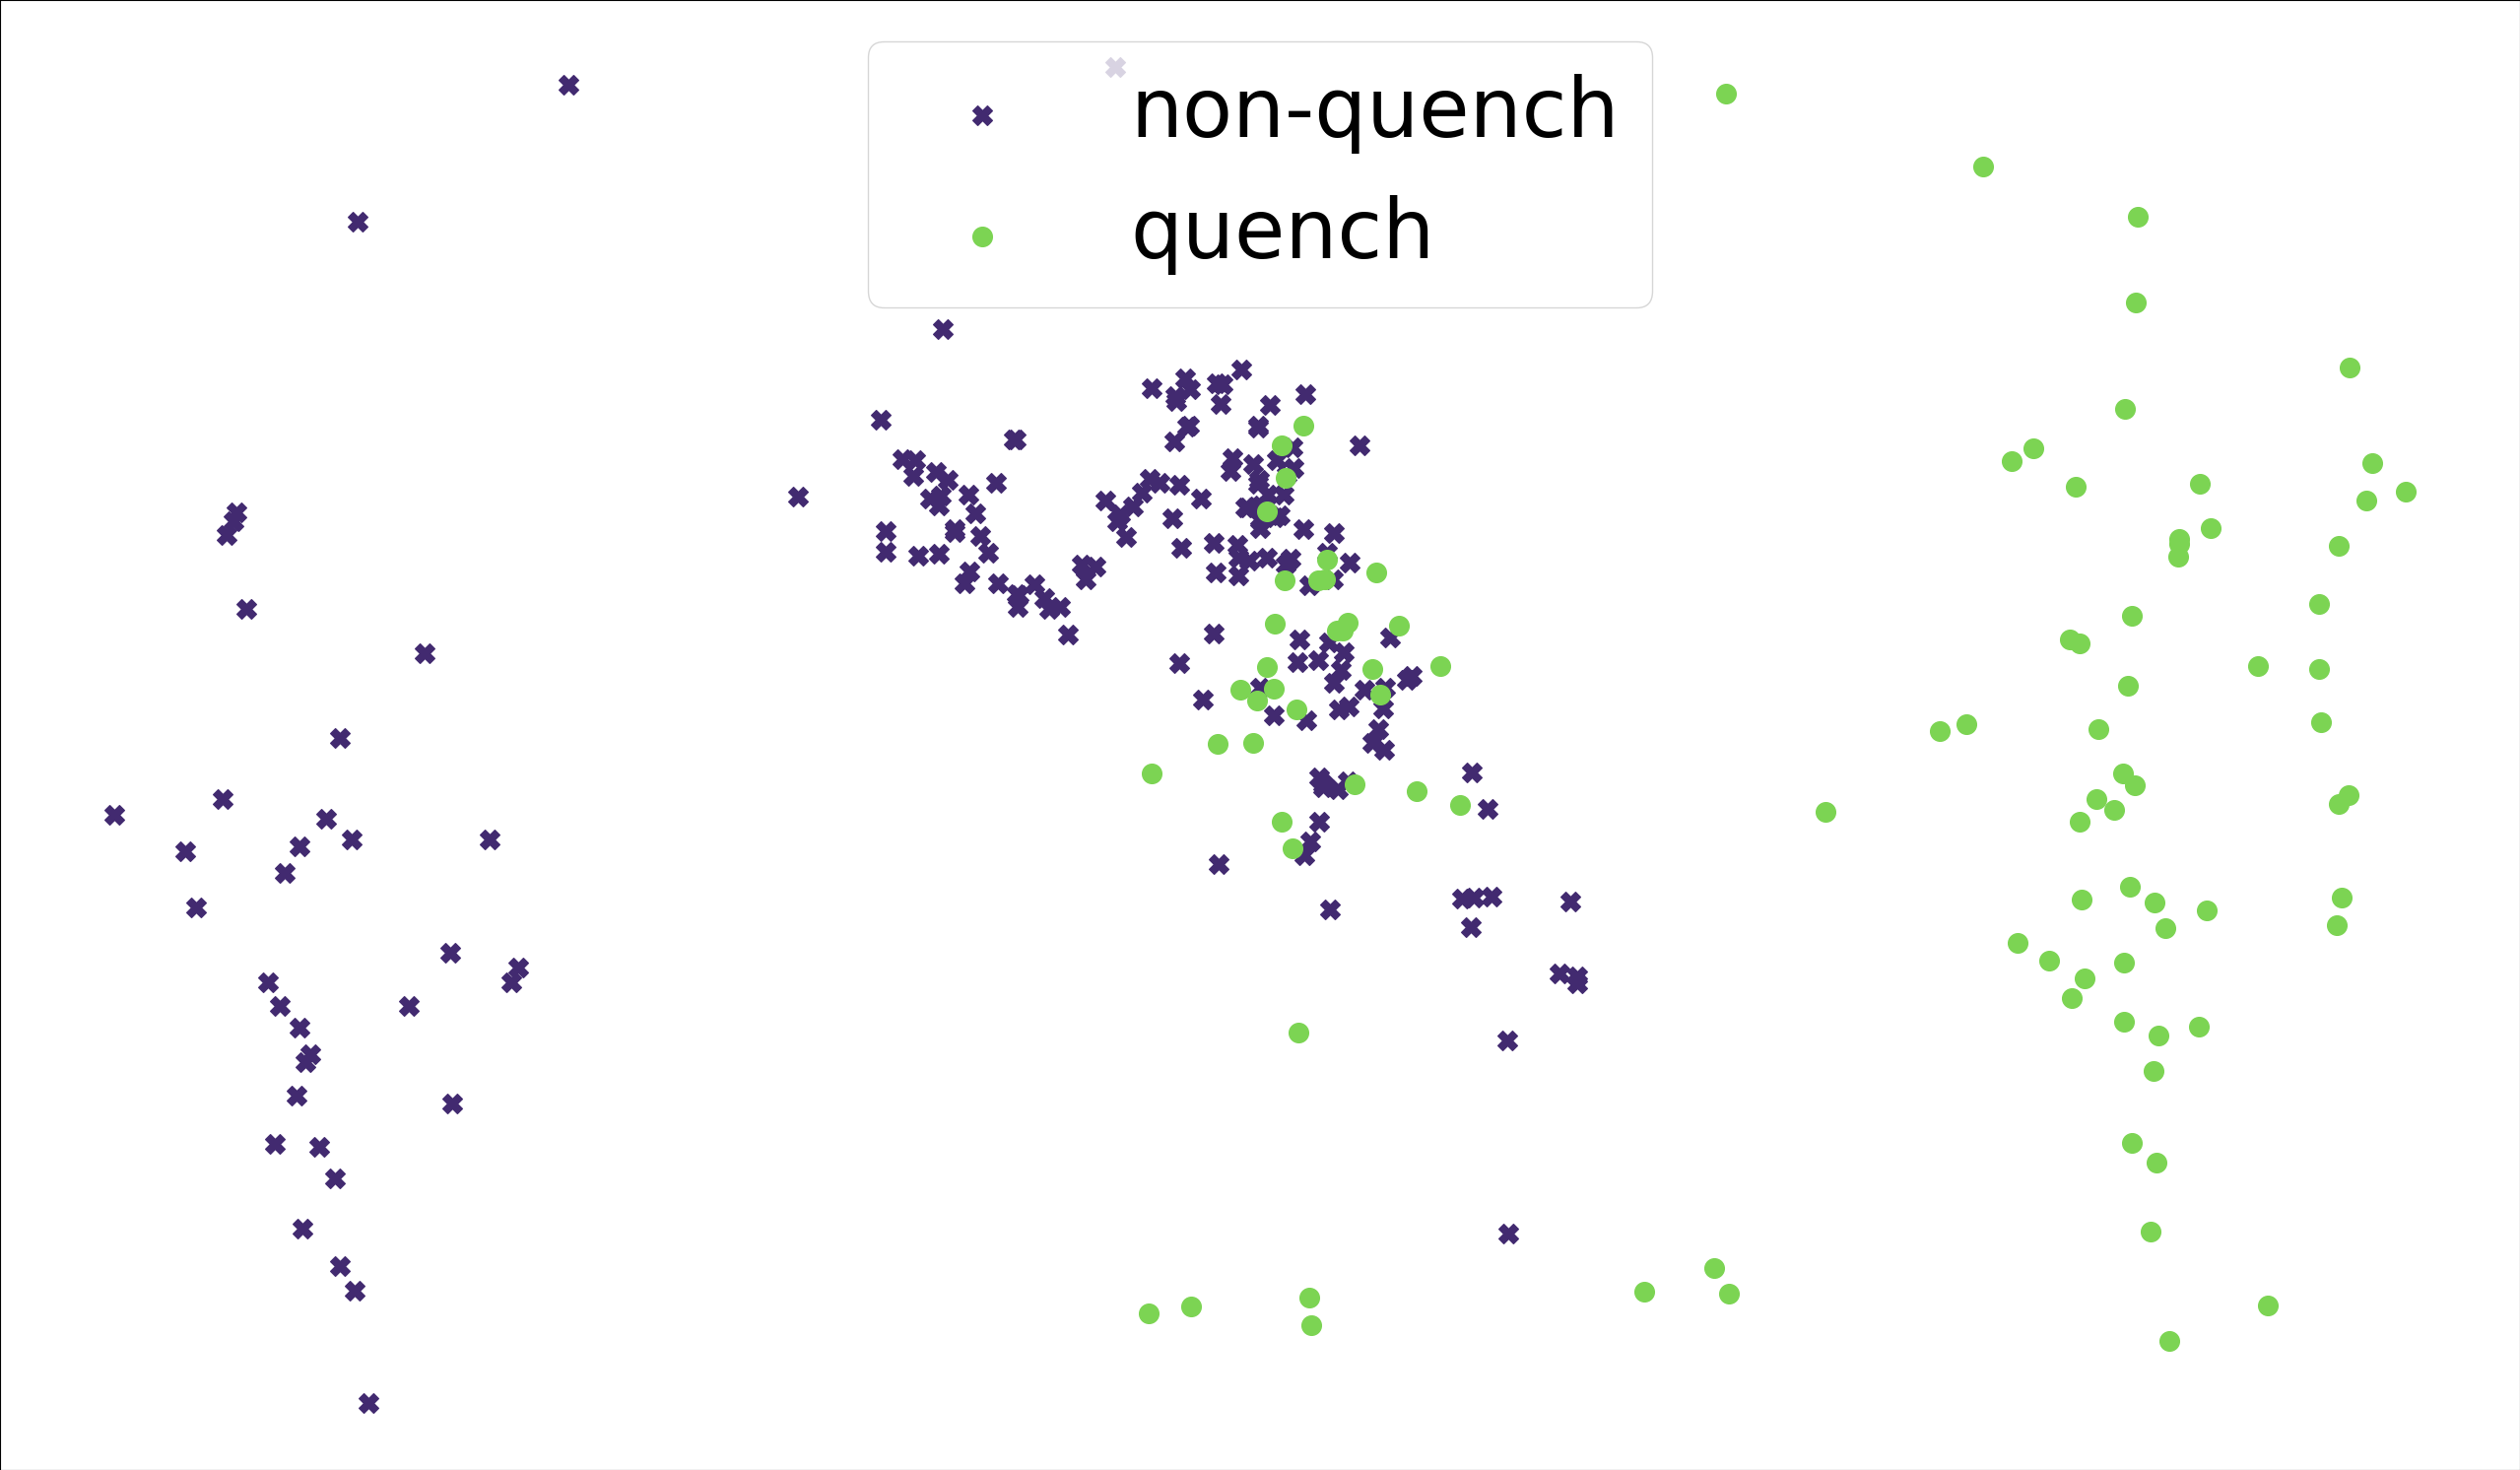
\includegraphics[width=\linewidth]{img/quench_dist_qlp/quenches_coil_1_Bn.png}
		\subcaption{}
	\end{subfigure}
	\begin{subfigure}{0.49\linewidth}
		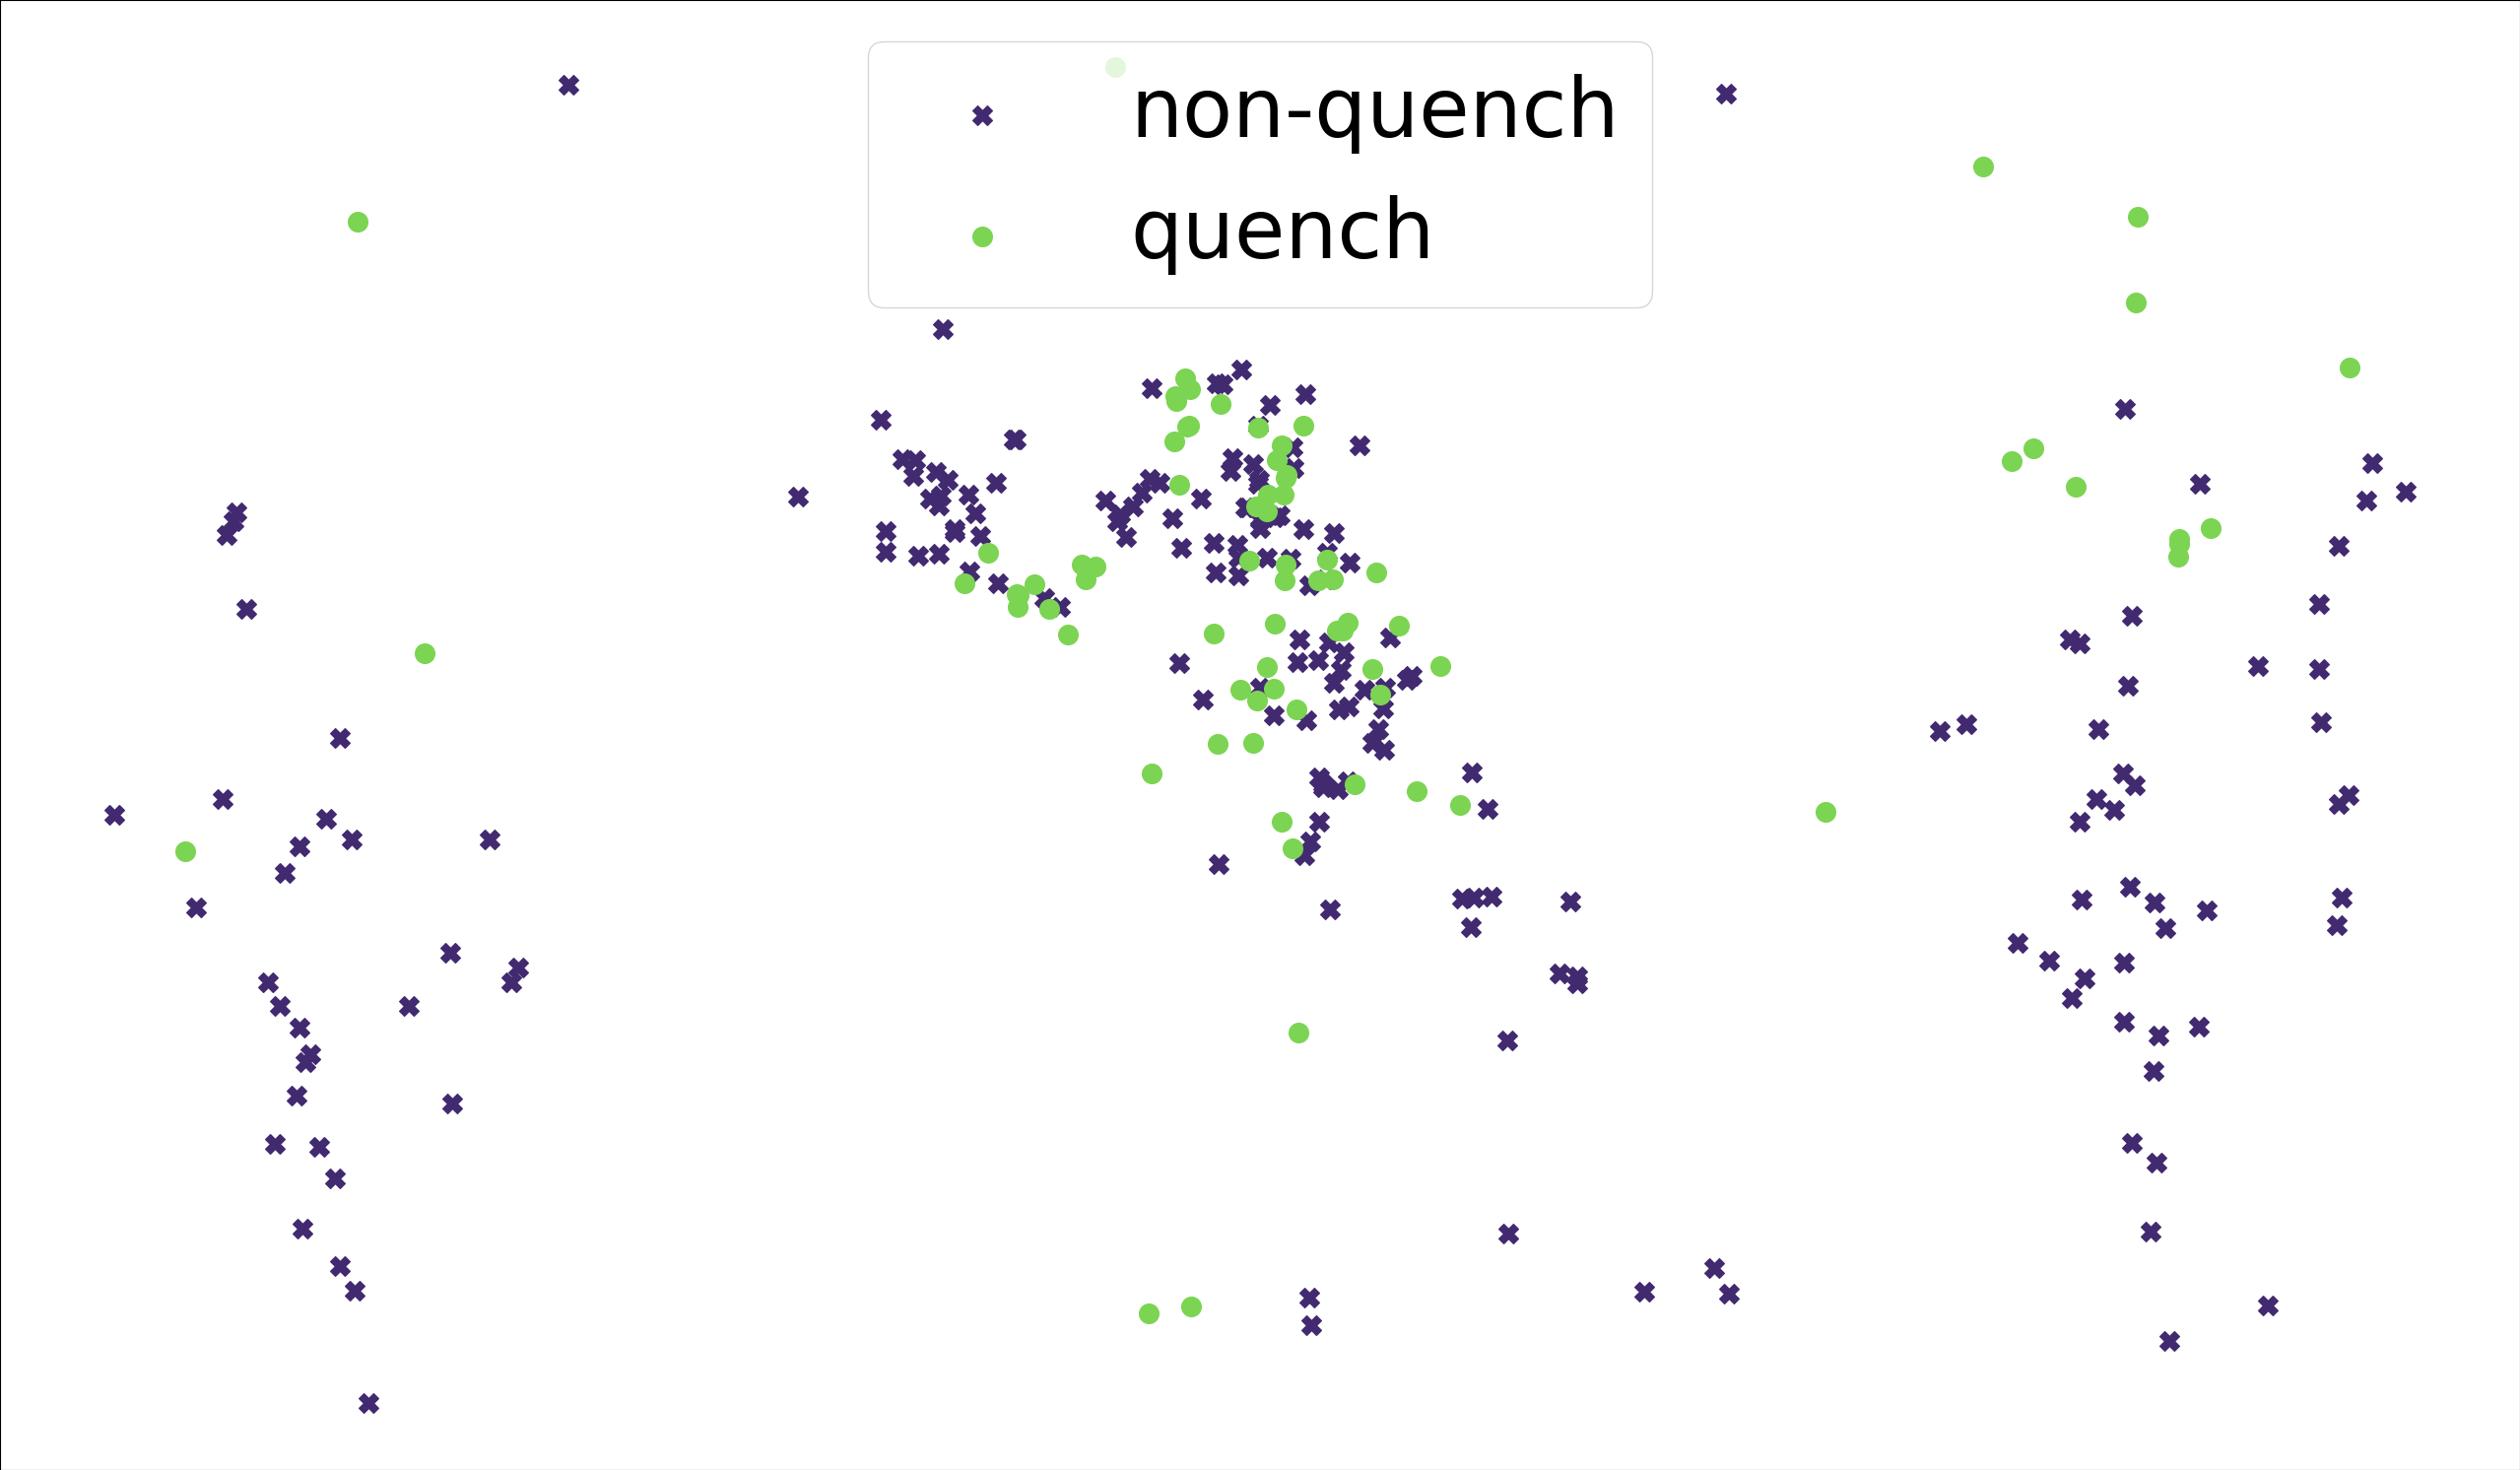
\includegraphics[width=\linewidth]{img/quench_dist_qlp/quenches_coil_2_Bn.png}
		\subcaption{}
	\end{subfigure}
	\begin{subfigure}{0.49\linewidth}
		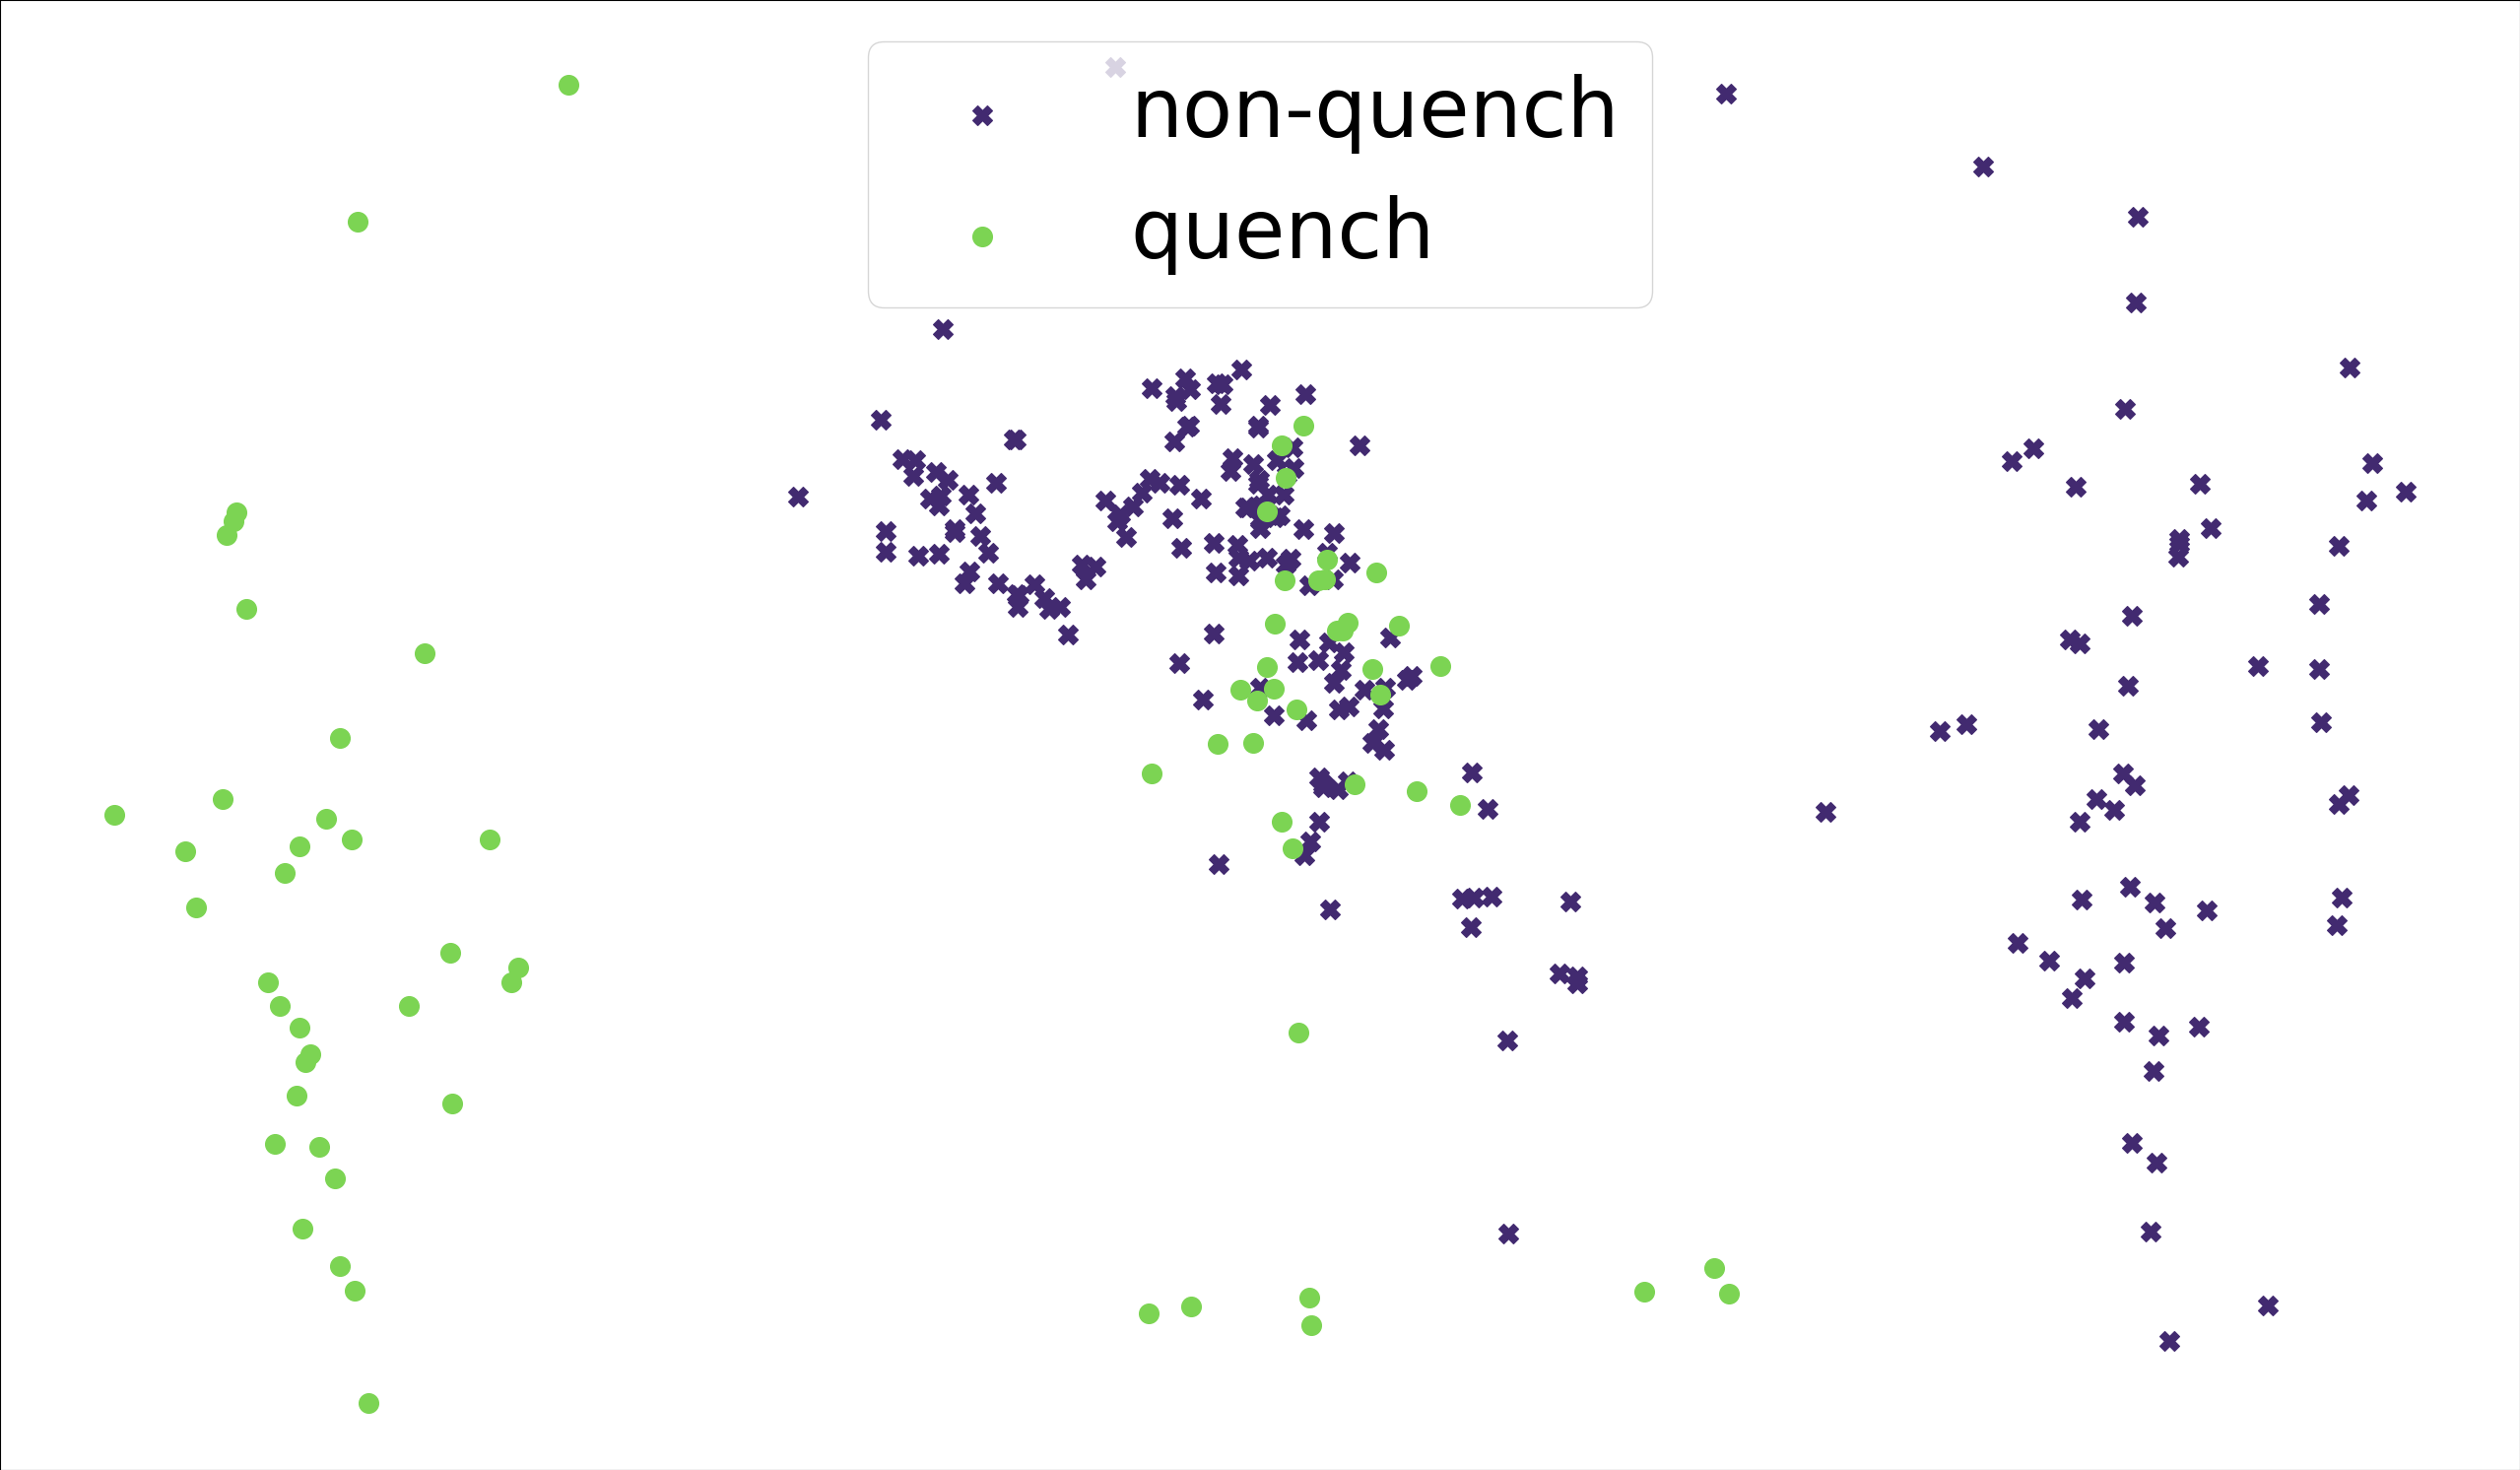
\includegraphics[width=\linewidth]{img/quench_dist_qlp/quenches_coil_3_Bn.png}
		\subcaption{}
	\end{subfigure}
	\caption{The distribution of the samples in bidimensional space after a round of \pca, for
		the \bn\ attribute. the subfigures contain different views of the same data: (a) differenciates between non-quench and single or multiple quench events, (b) highlights the distribution of quenches for coil $0$, (c) highlights the distribution of quenches for coil $1$, (d) highlights the distribution of quenches for coil $2$ and finally (e) highlights the distribution of quenches for coil $3$.}
	\label{fig:bn-coilq-dist}
\end{figure}

\subsubsection{\cnmod}
As we said in \Cref{chp:problem}, \cnmod\ was expected to be very informative for \qrp, but not for
\qlp. Interestingly, though, the correlation between the harmonics for the attribute and the labels
associated to each coil, shown in \Cref{fig:cnmod-lcorr-qlp}, seem to be telling a different story.
If we consider coils $0$ and $3$, we can see a very strong correlation between the harmonics and the
label, it's also worth noting that in all the sub-figures, \cnmod[2]\ seems to be extremely
important to explain the value associated with the labels.

If we look back at the correlation matrix computed for \cnmod\ during the preprocessing for \qrp\
(see \Cref{fig:cnmod-corr}) we could say that the structure of a sub-view of \cnmod\ could be built:
\begin{itemize}
	\item in the case of coil $0$, \cnmod[2] and adding a high-order candidate.
	      While this would technically maximize the total correlation with the label, we have
	      seen in \qrp\ that choosing \cnmod[2]\ was a choice that didn't pay. That
	      is why we should be using \cnmod[3], \cnmod[6] and another high order harmonics like \cnmod[9] or \cnmod[11].
	\item in the case of coil $3$, we could be taking harmonic \cnmod[1] and then using one or
	      more from \{\cnmod[4], \cnmod[5], \cnmod[6], \cnmod[7], \cnmod[8]\}; finally, if it makes performance better, we could also add
	      another high order harmonic like \cnmod[10].
\end{itemize}
\begin{figure}[!ht]
	% Font size = 70
	\centering
	\begin{subfigure}{0.49\linewidth}
		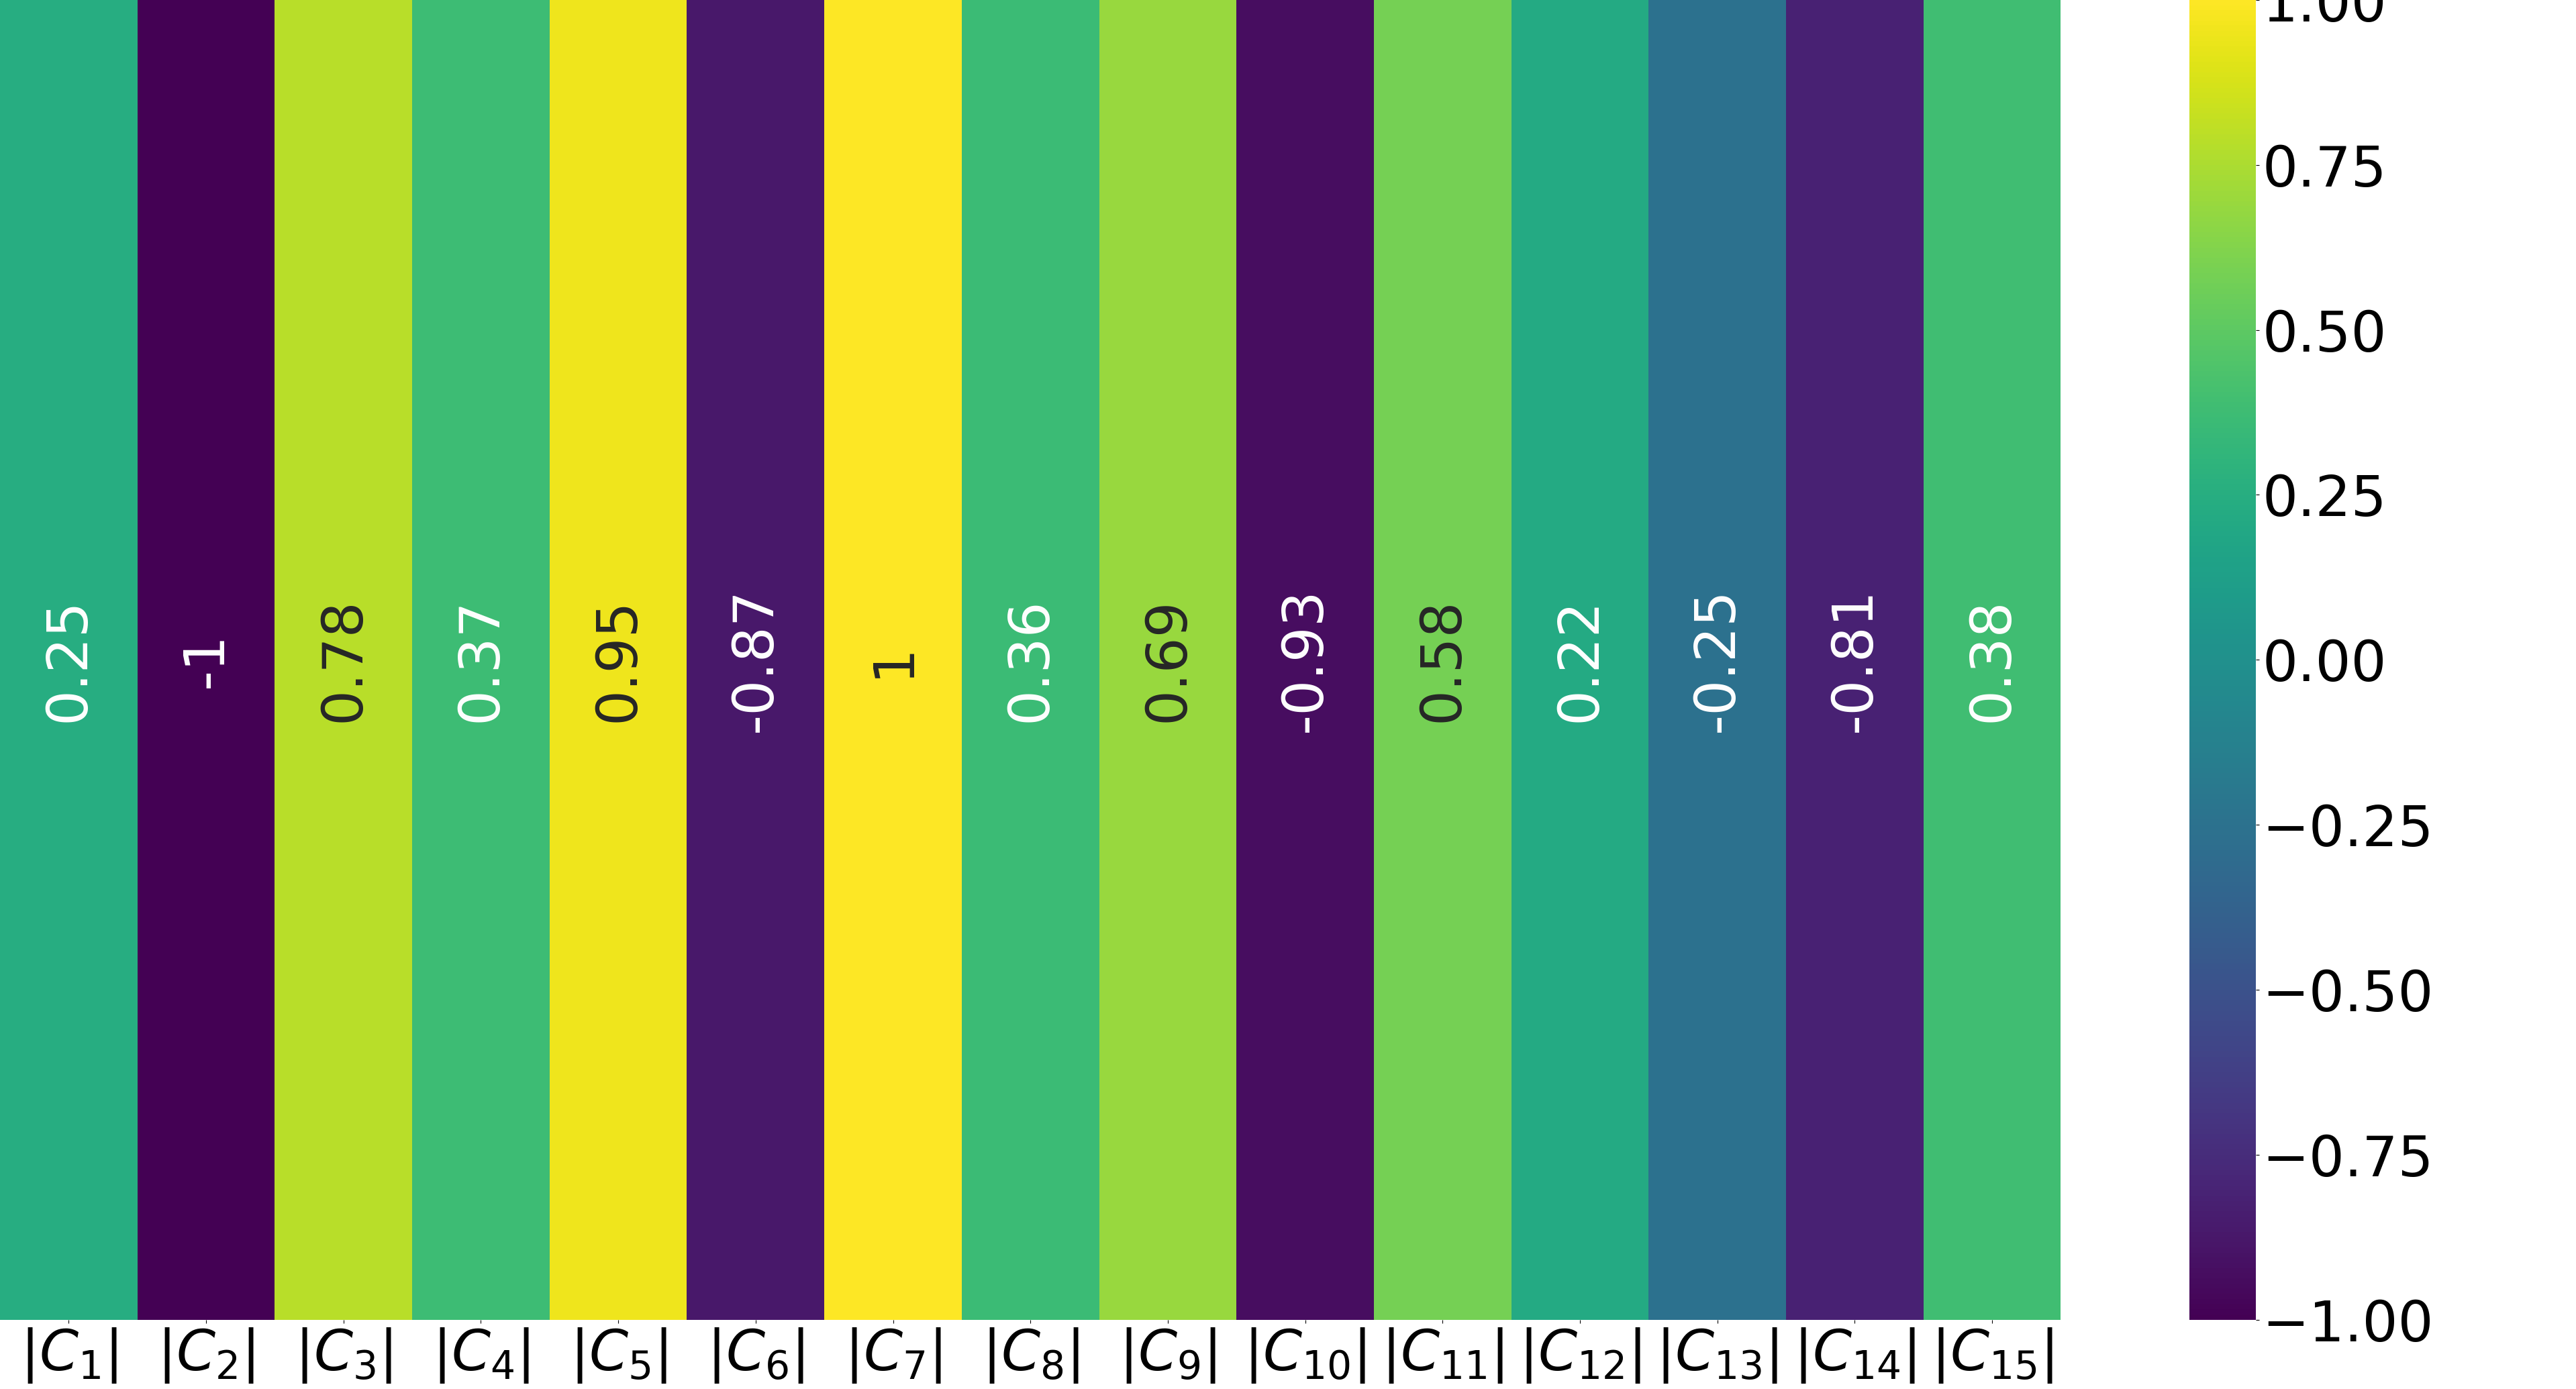
\includegraphics[width=\linewidth]{img/qlp_corr/Cnmod_coil0.png}
		\subcaption{Correlation with coil $0$}
	\end{subfigure}
	\begin{subfigure}{0.49\linewidth}
		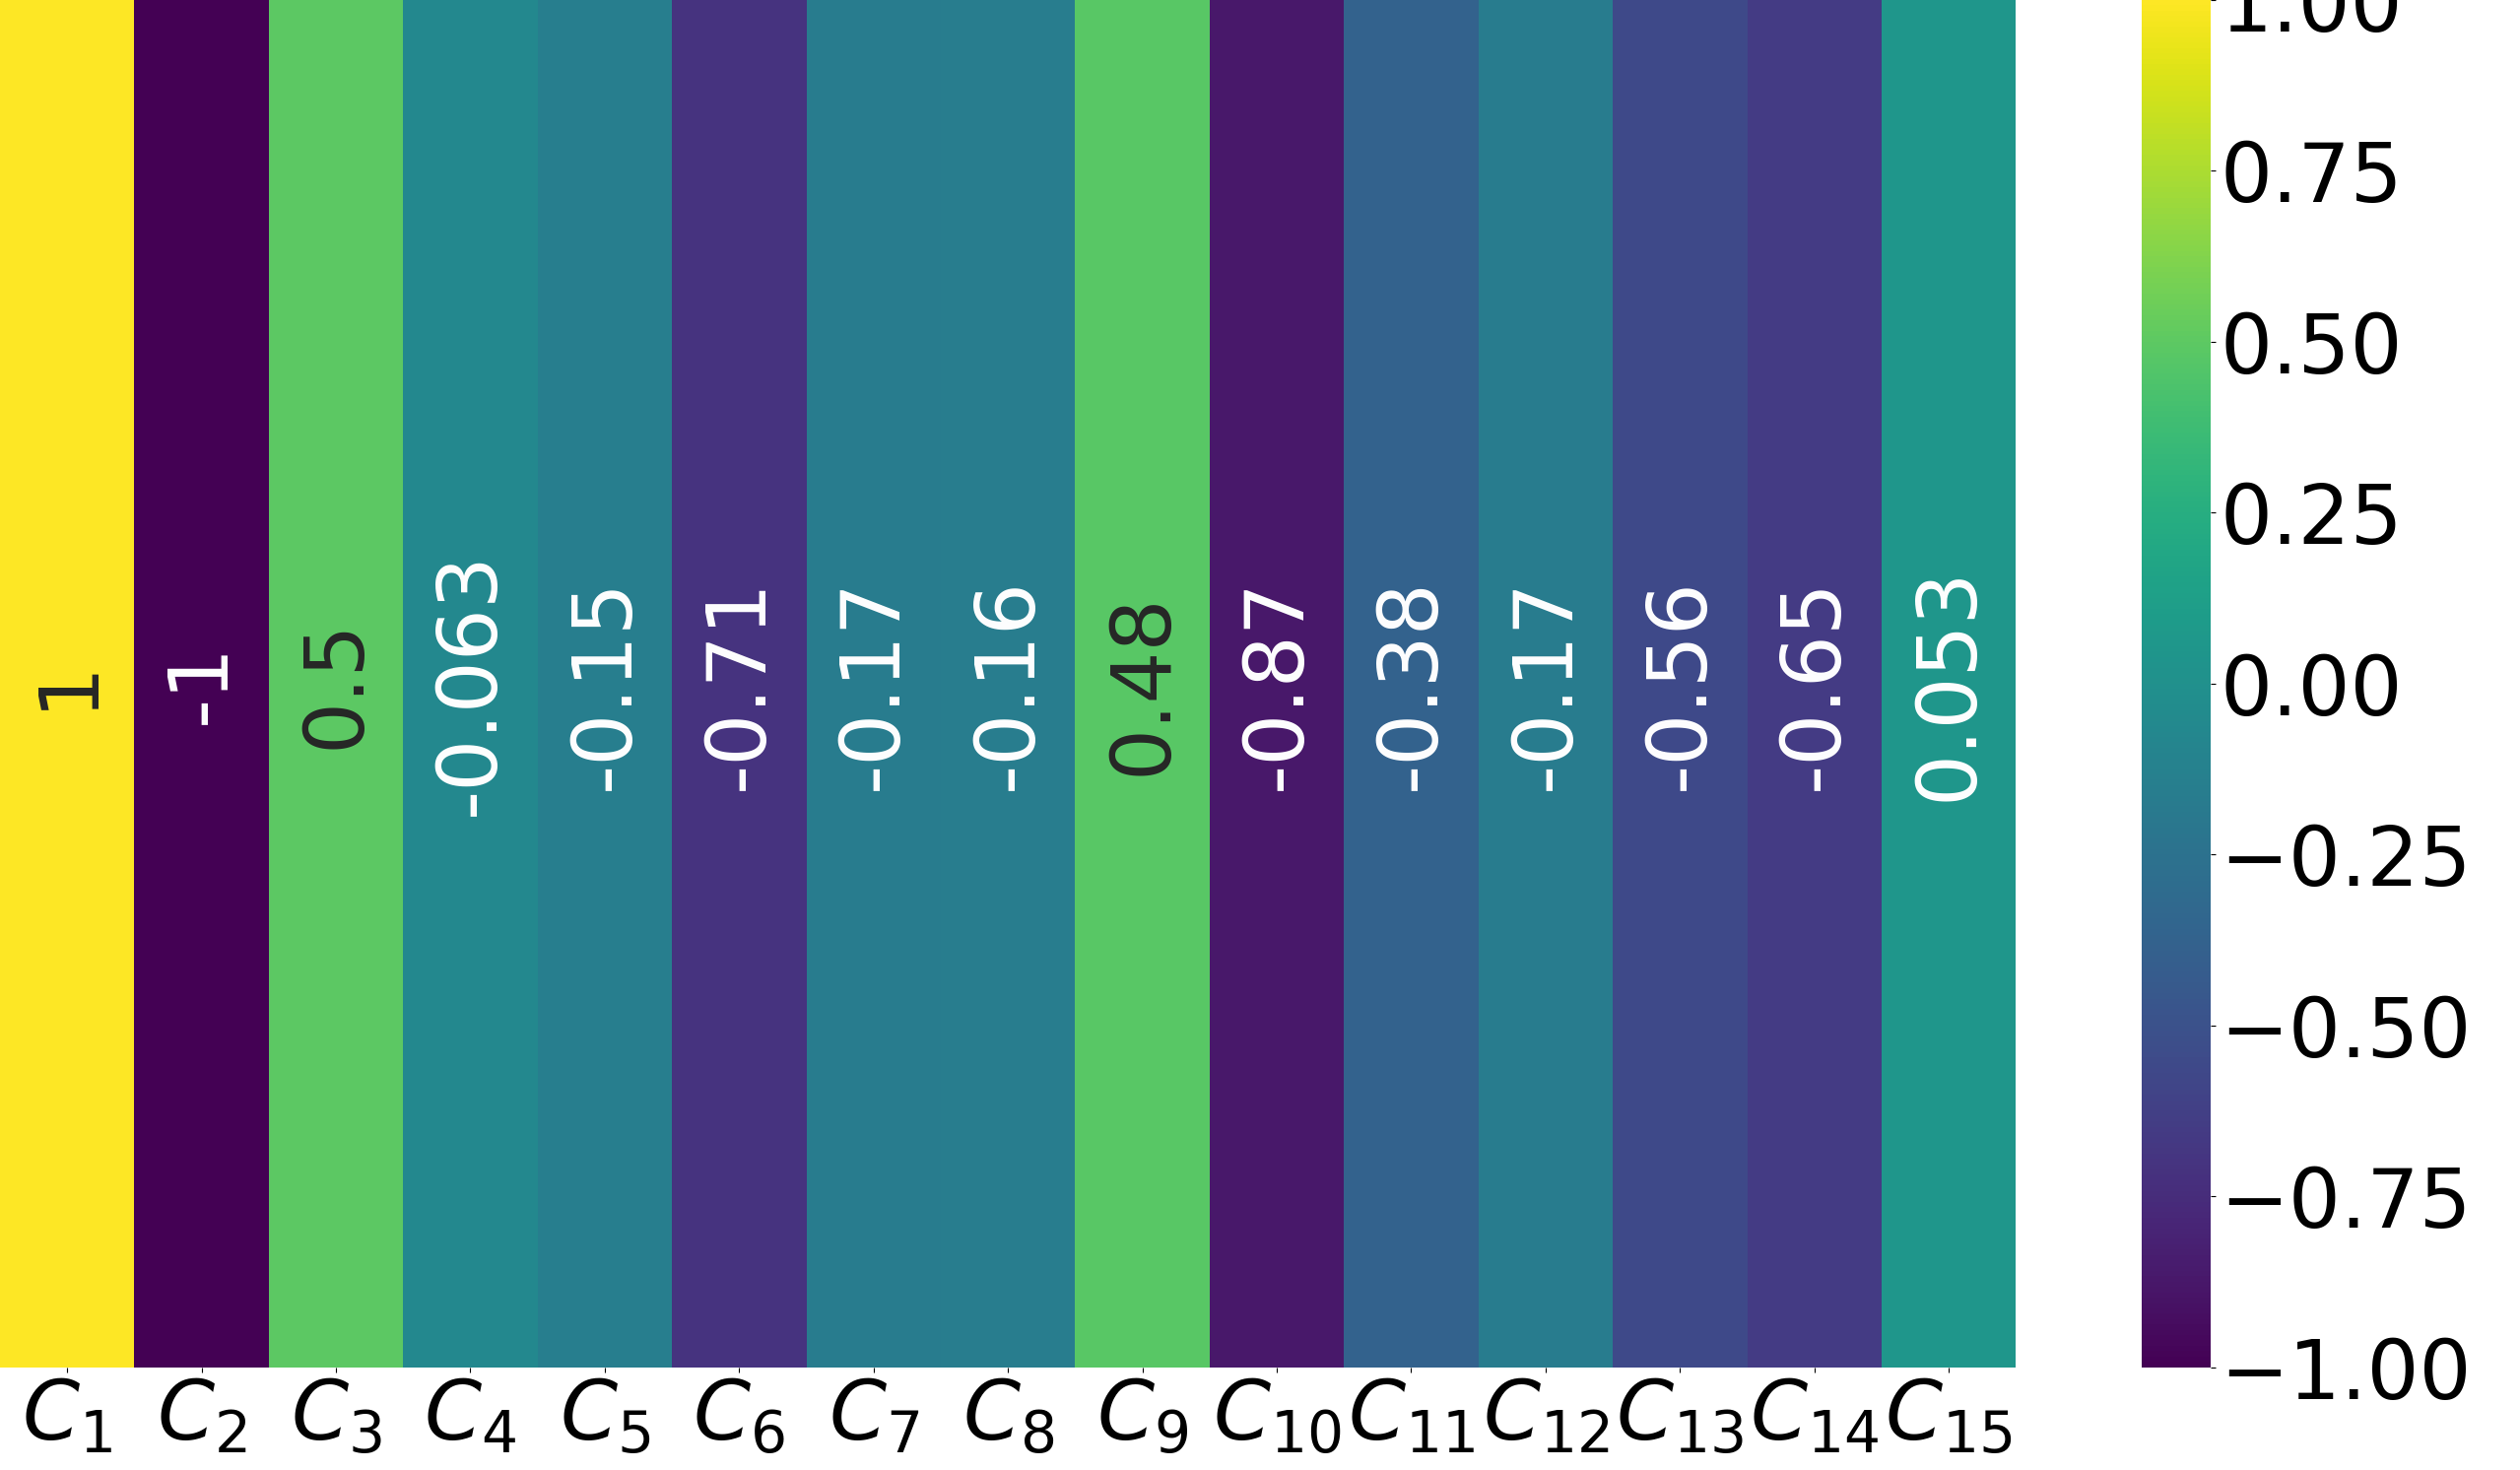
\includegraphics[width=\linewidth]{img/qlp_corr/Cnmod_coil1.png}
		\subcaption{Correlation with coil $1$}
	\end{subfigure}
	\begin{subfigure}{0.49\linewidth}
		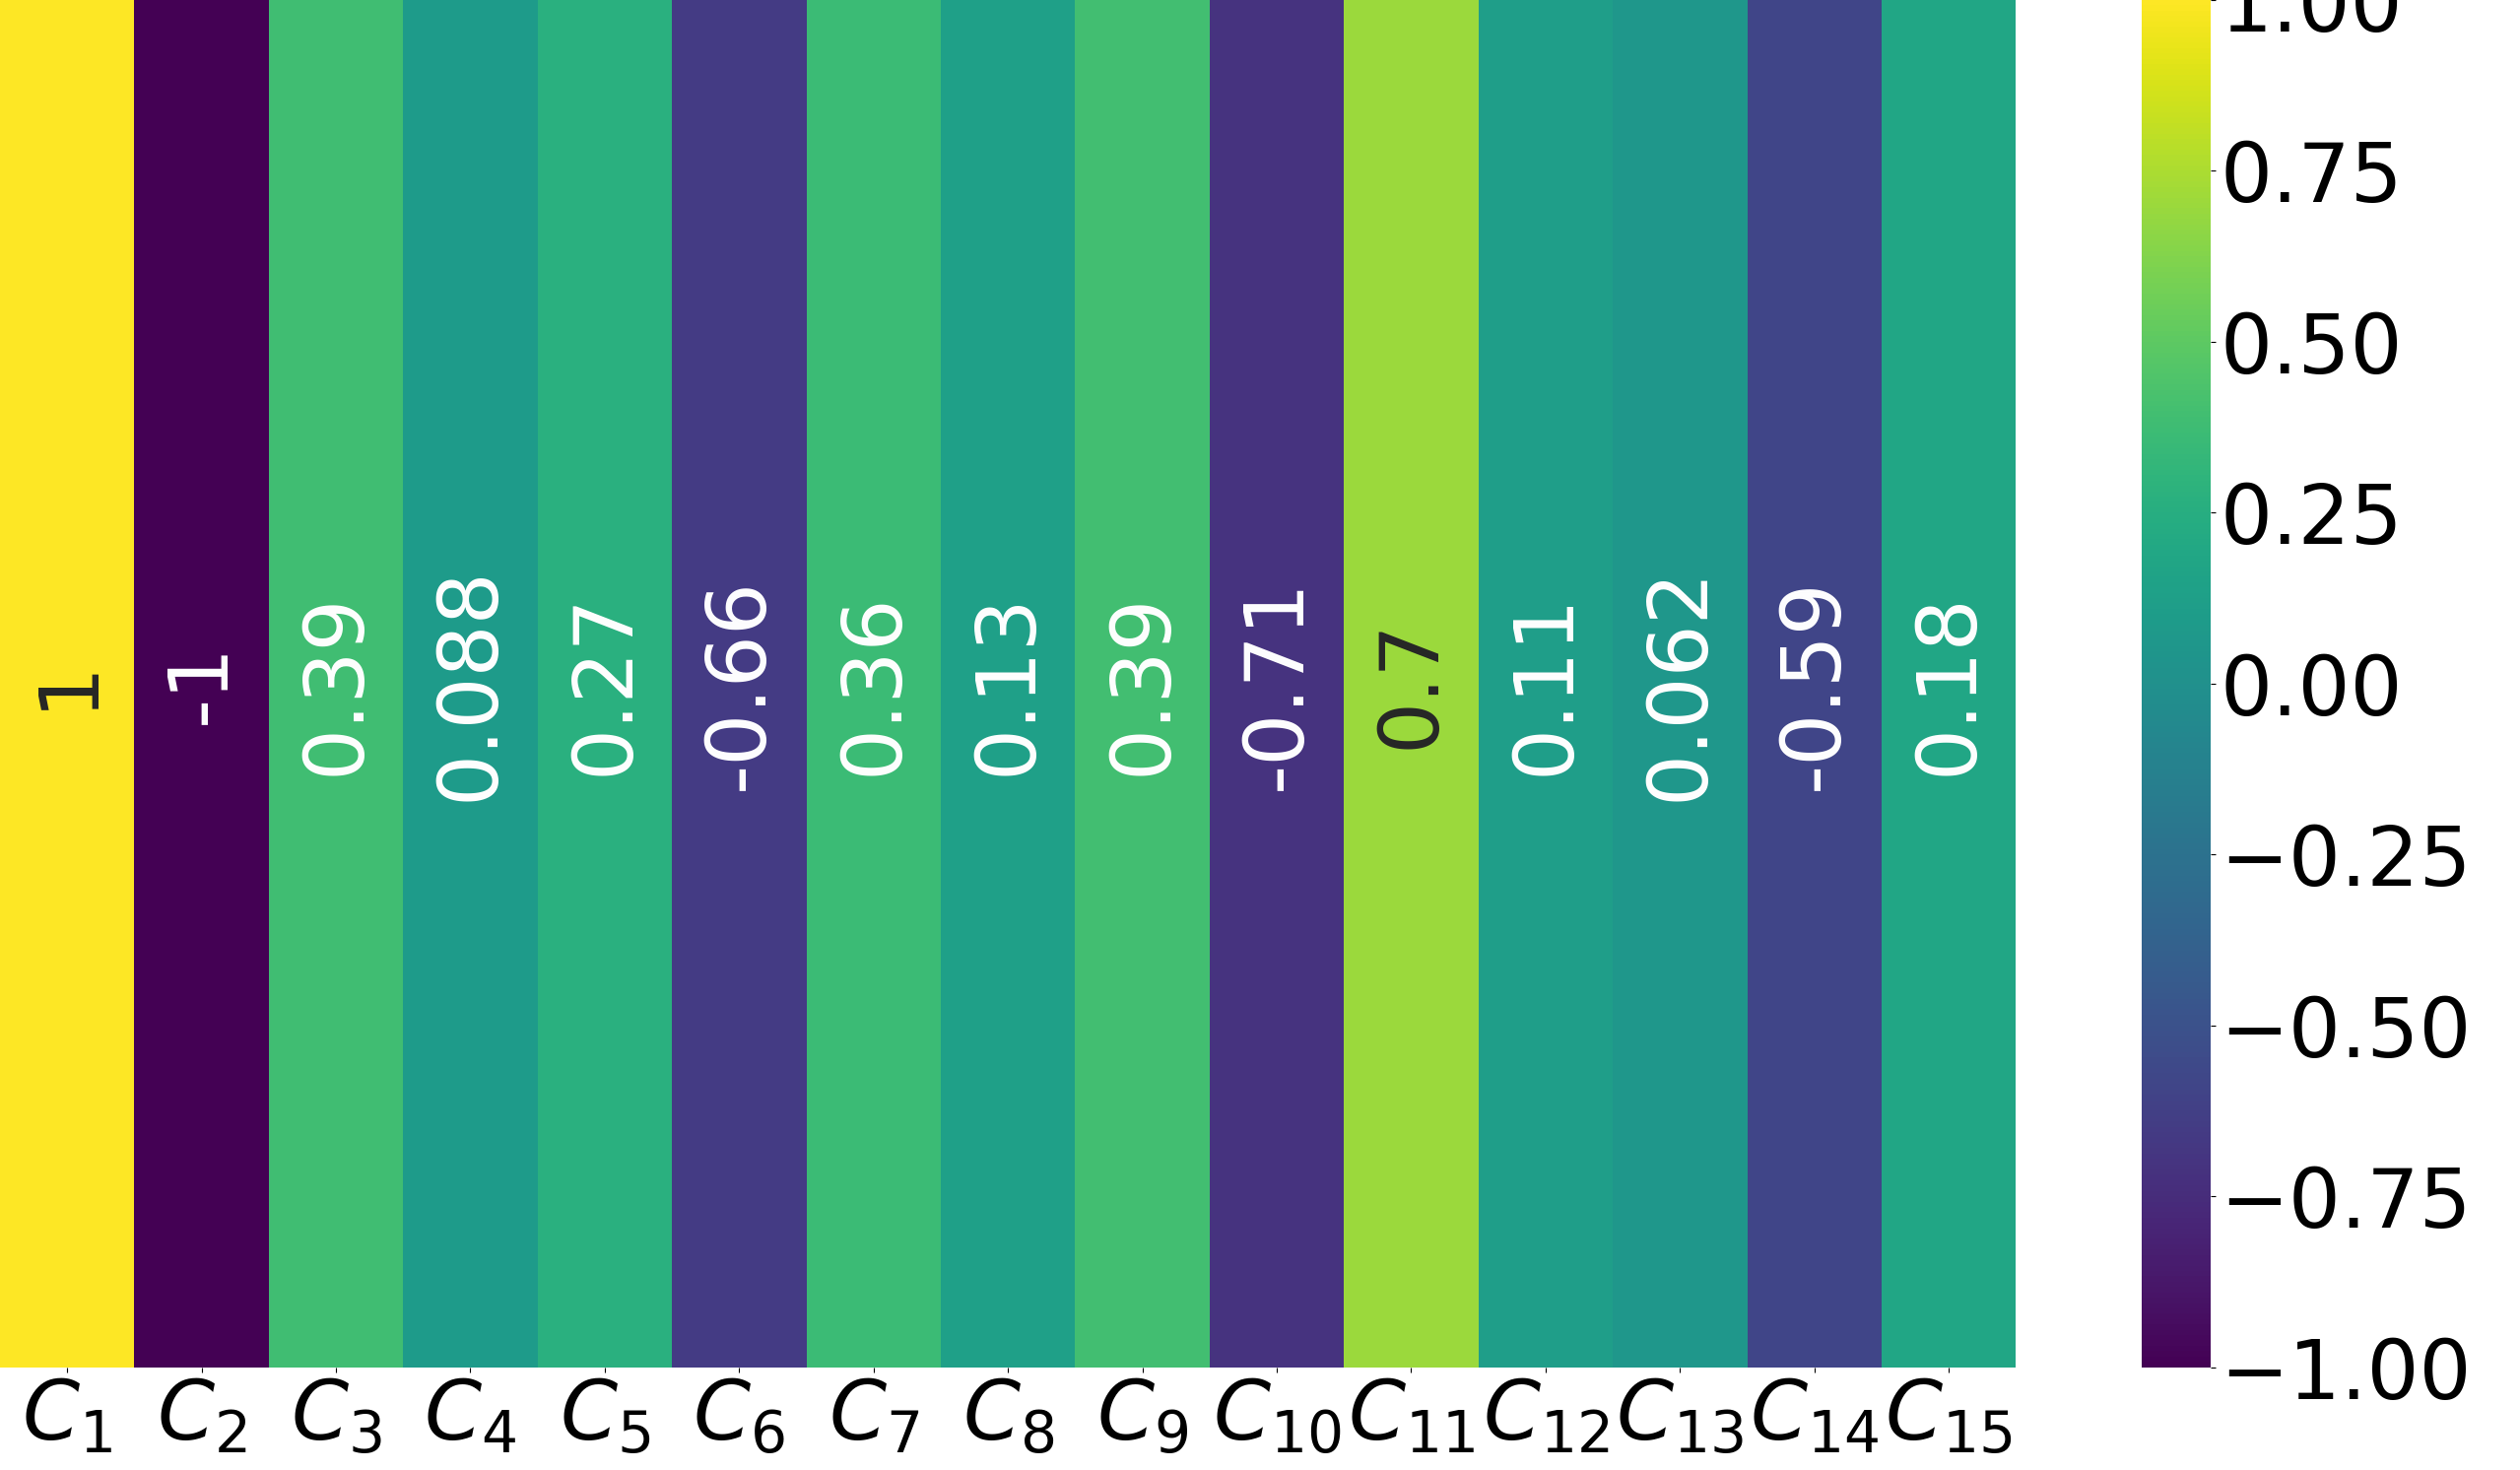
\includegraphics[width=\linewidth]{img/qlp_corr/Cnmod_coil2.png}
		\subcaption{Correlation with coil $2$}
	\end{subfigure}
	\begin{subfigure}{0.49\linewidth}
		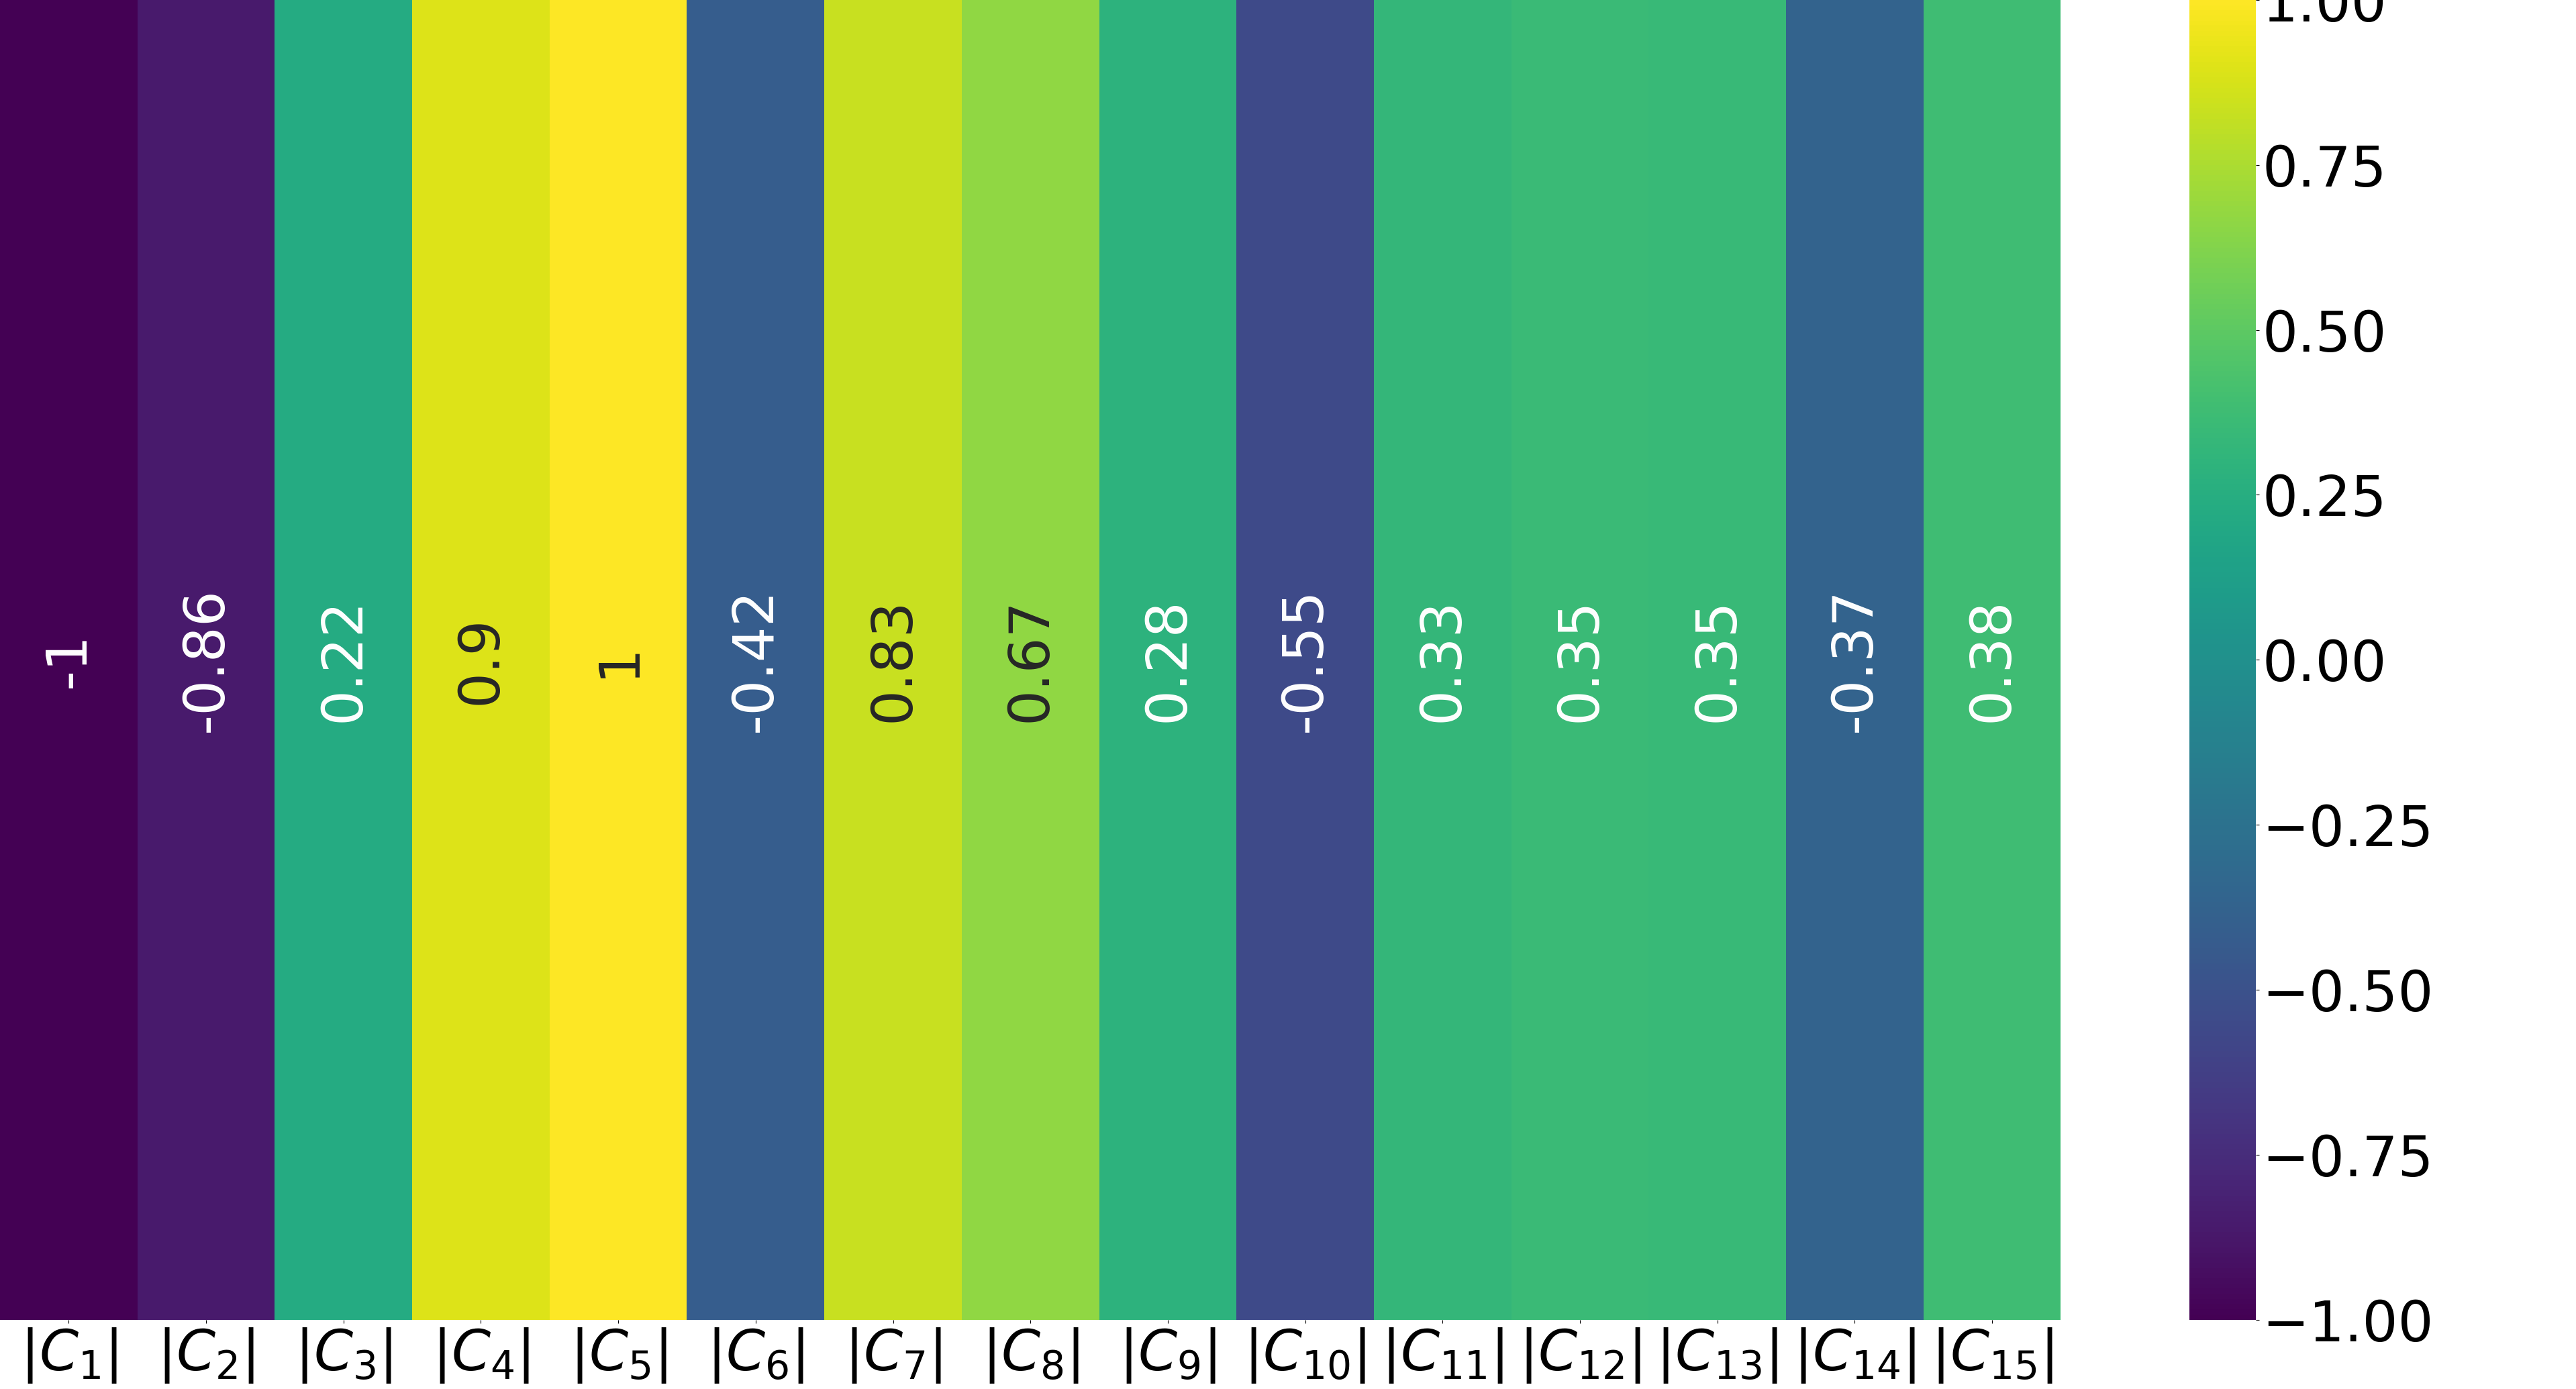
\includegraphics[width=\linewidth]{img/qlp_corr/Cnmod_coil3.png}
		\subcaption{Correlation with coil $3$}
	\end{subfigure}
	\caption{Correlation between the harmonics of the \cnmod\ attribute and the labels for \qlp.}
	\label{fig:cnmod-lcorr-qlp}
\end{figure}

As we did for \an\ and \bn, we visualized the distribution of the data after a round of \pca\
dimensionality reduction. \Cref{fig:cnmod-coilq-dist} shows a similar situation to \an, if we
consider the specific case of sub-figure (a), while the clusters are not as clean cut, as the
alternative, there is much more separation of the classes compared to \bn.
As far as single coil quench is concerned (subfigures (b) - (e)), we can see, in most cases, a high
level of homogeneity of quench and non-quench samples.

\begin{figure}[!ht]
	% Font size = 70
	\centering
	\begin{subfigure}{\linewidth}
		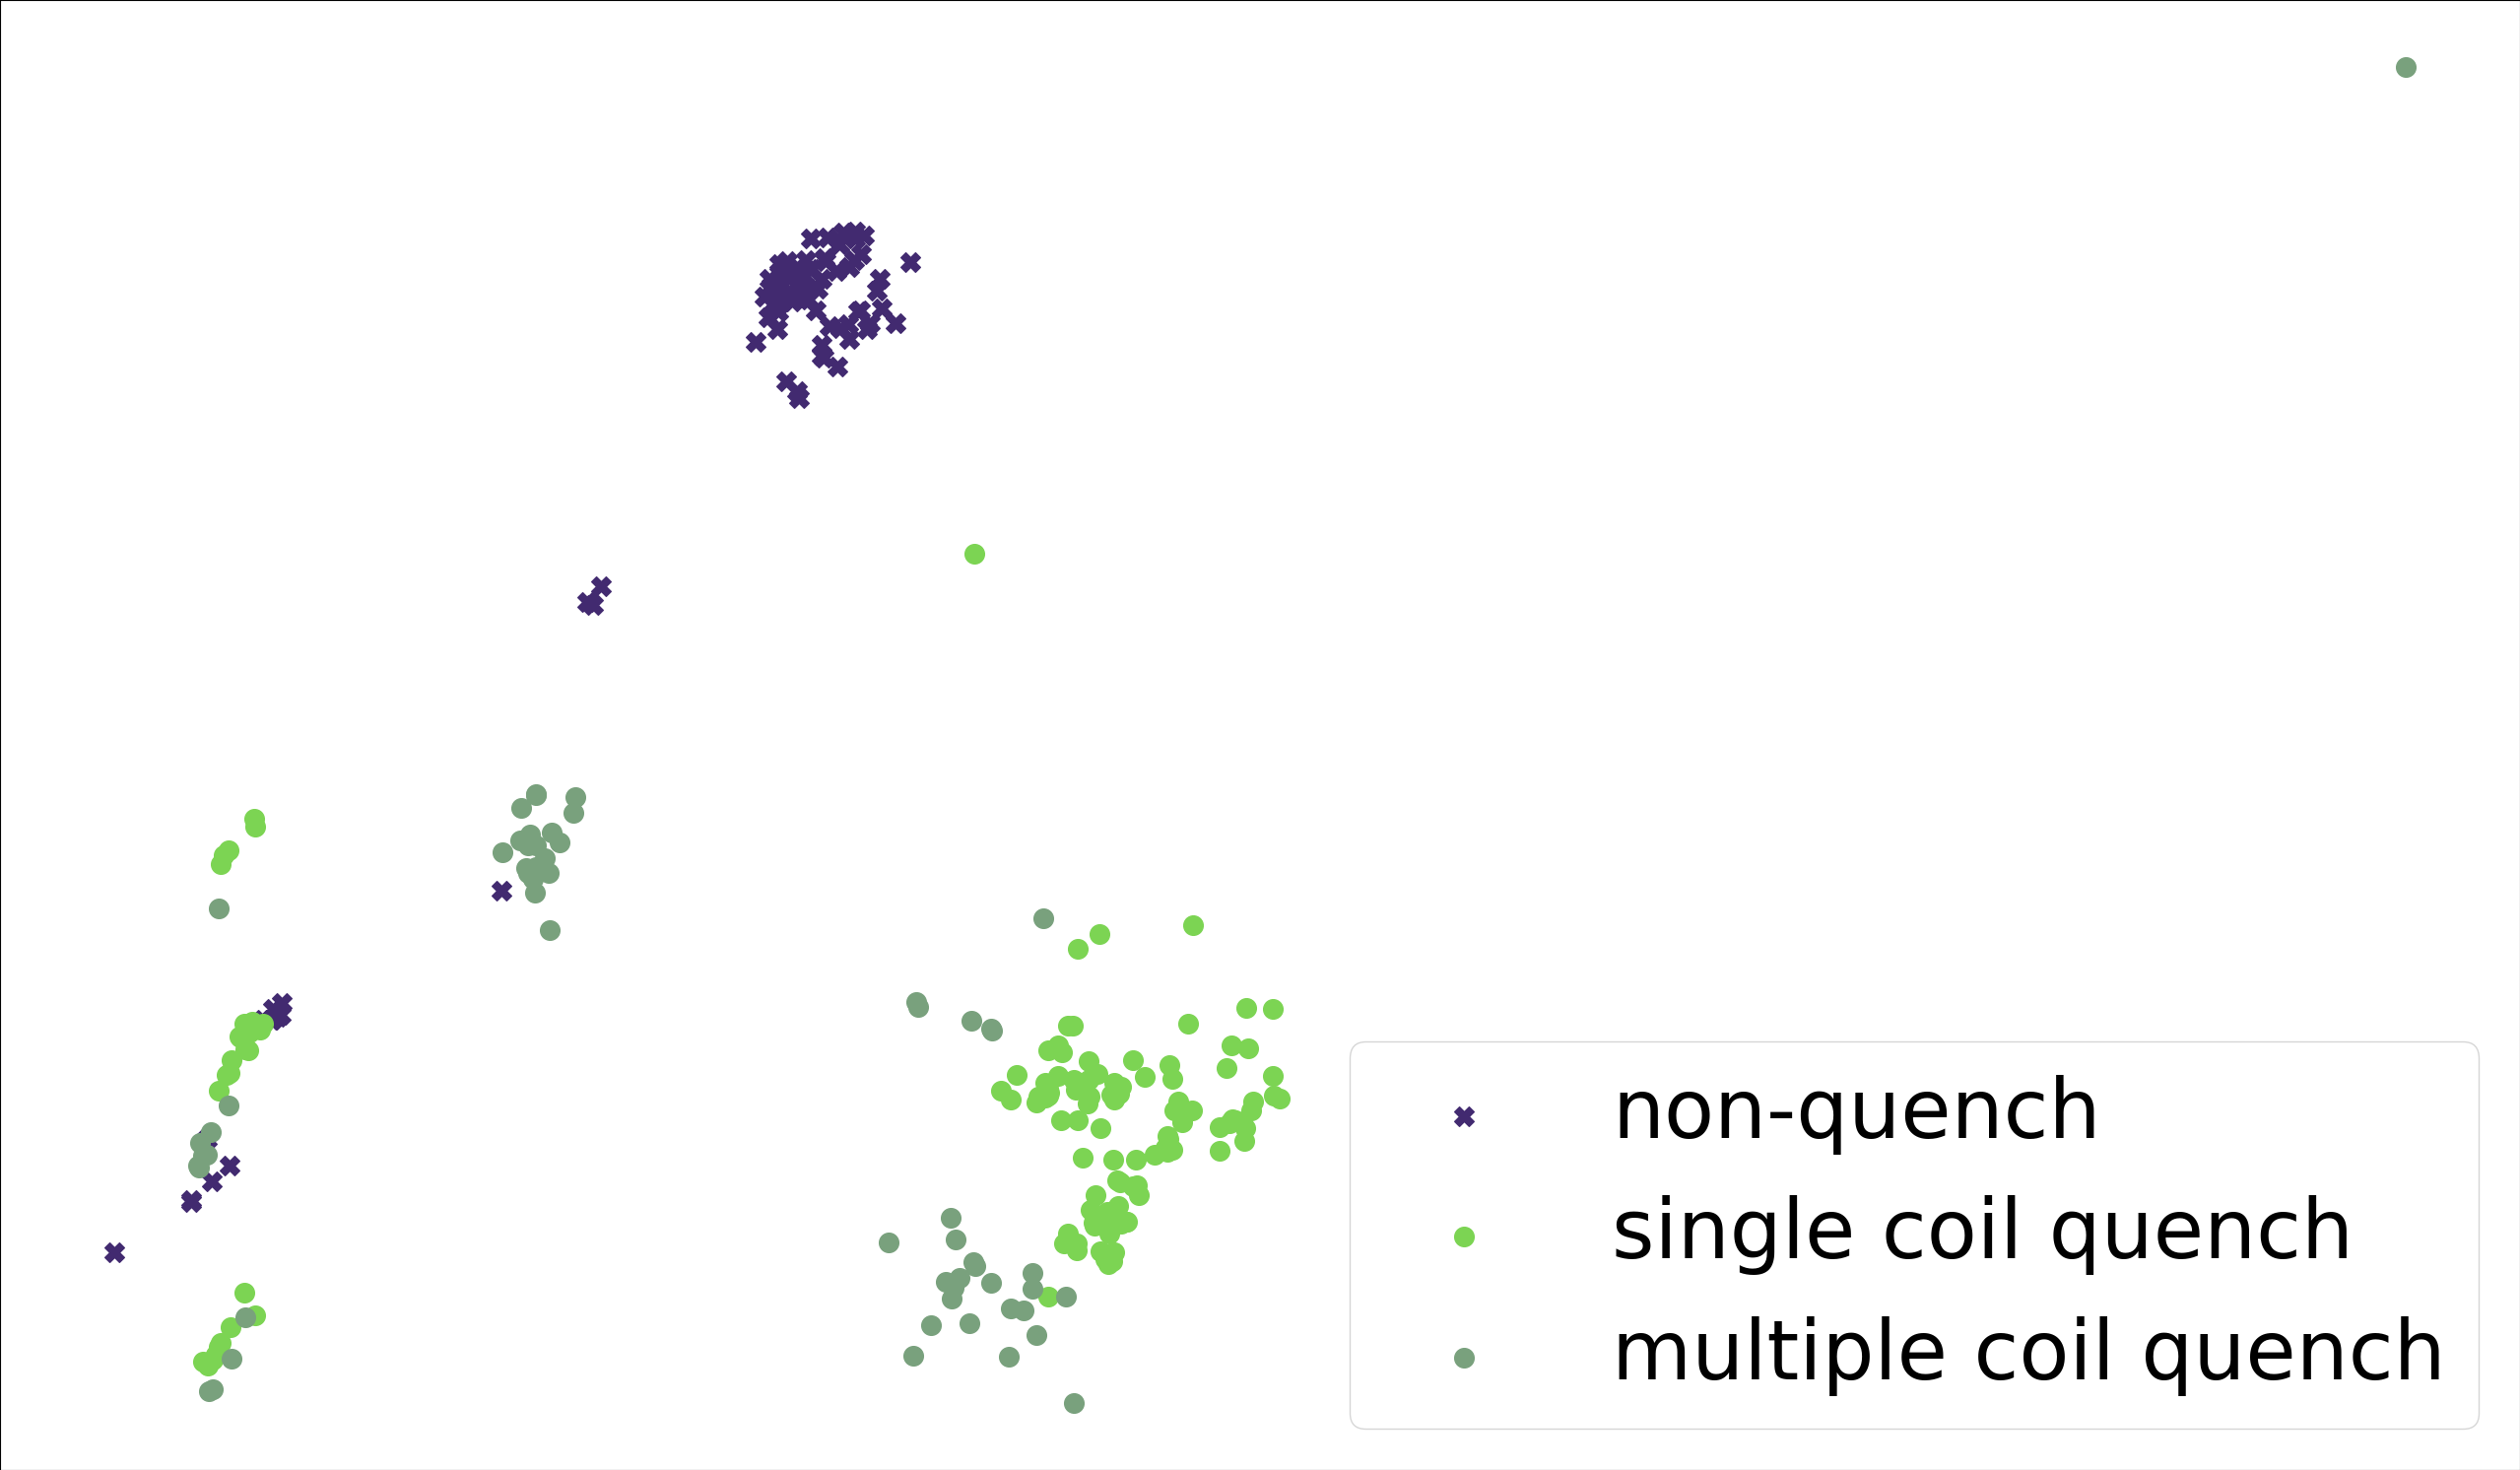
\includegraphics[width=\linewidth]{img/quench_dist_qlp/single_vs_multiple_Cnmod.png}
		\subcaption{}
	\end{subfigure}
	\begin{subfigure}{0.49\linewidth}
		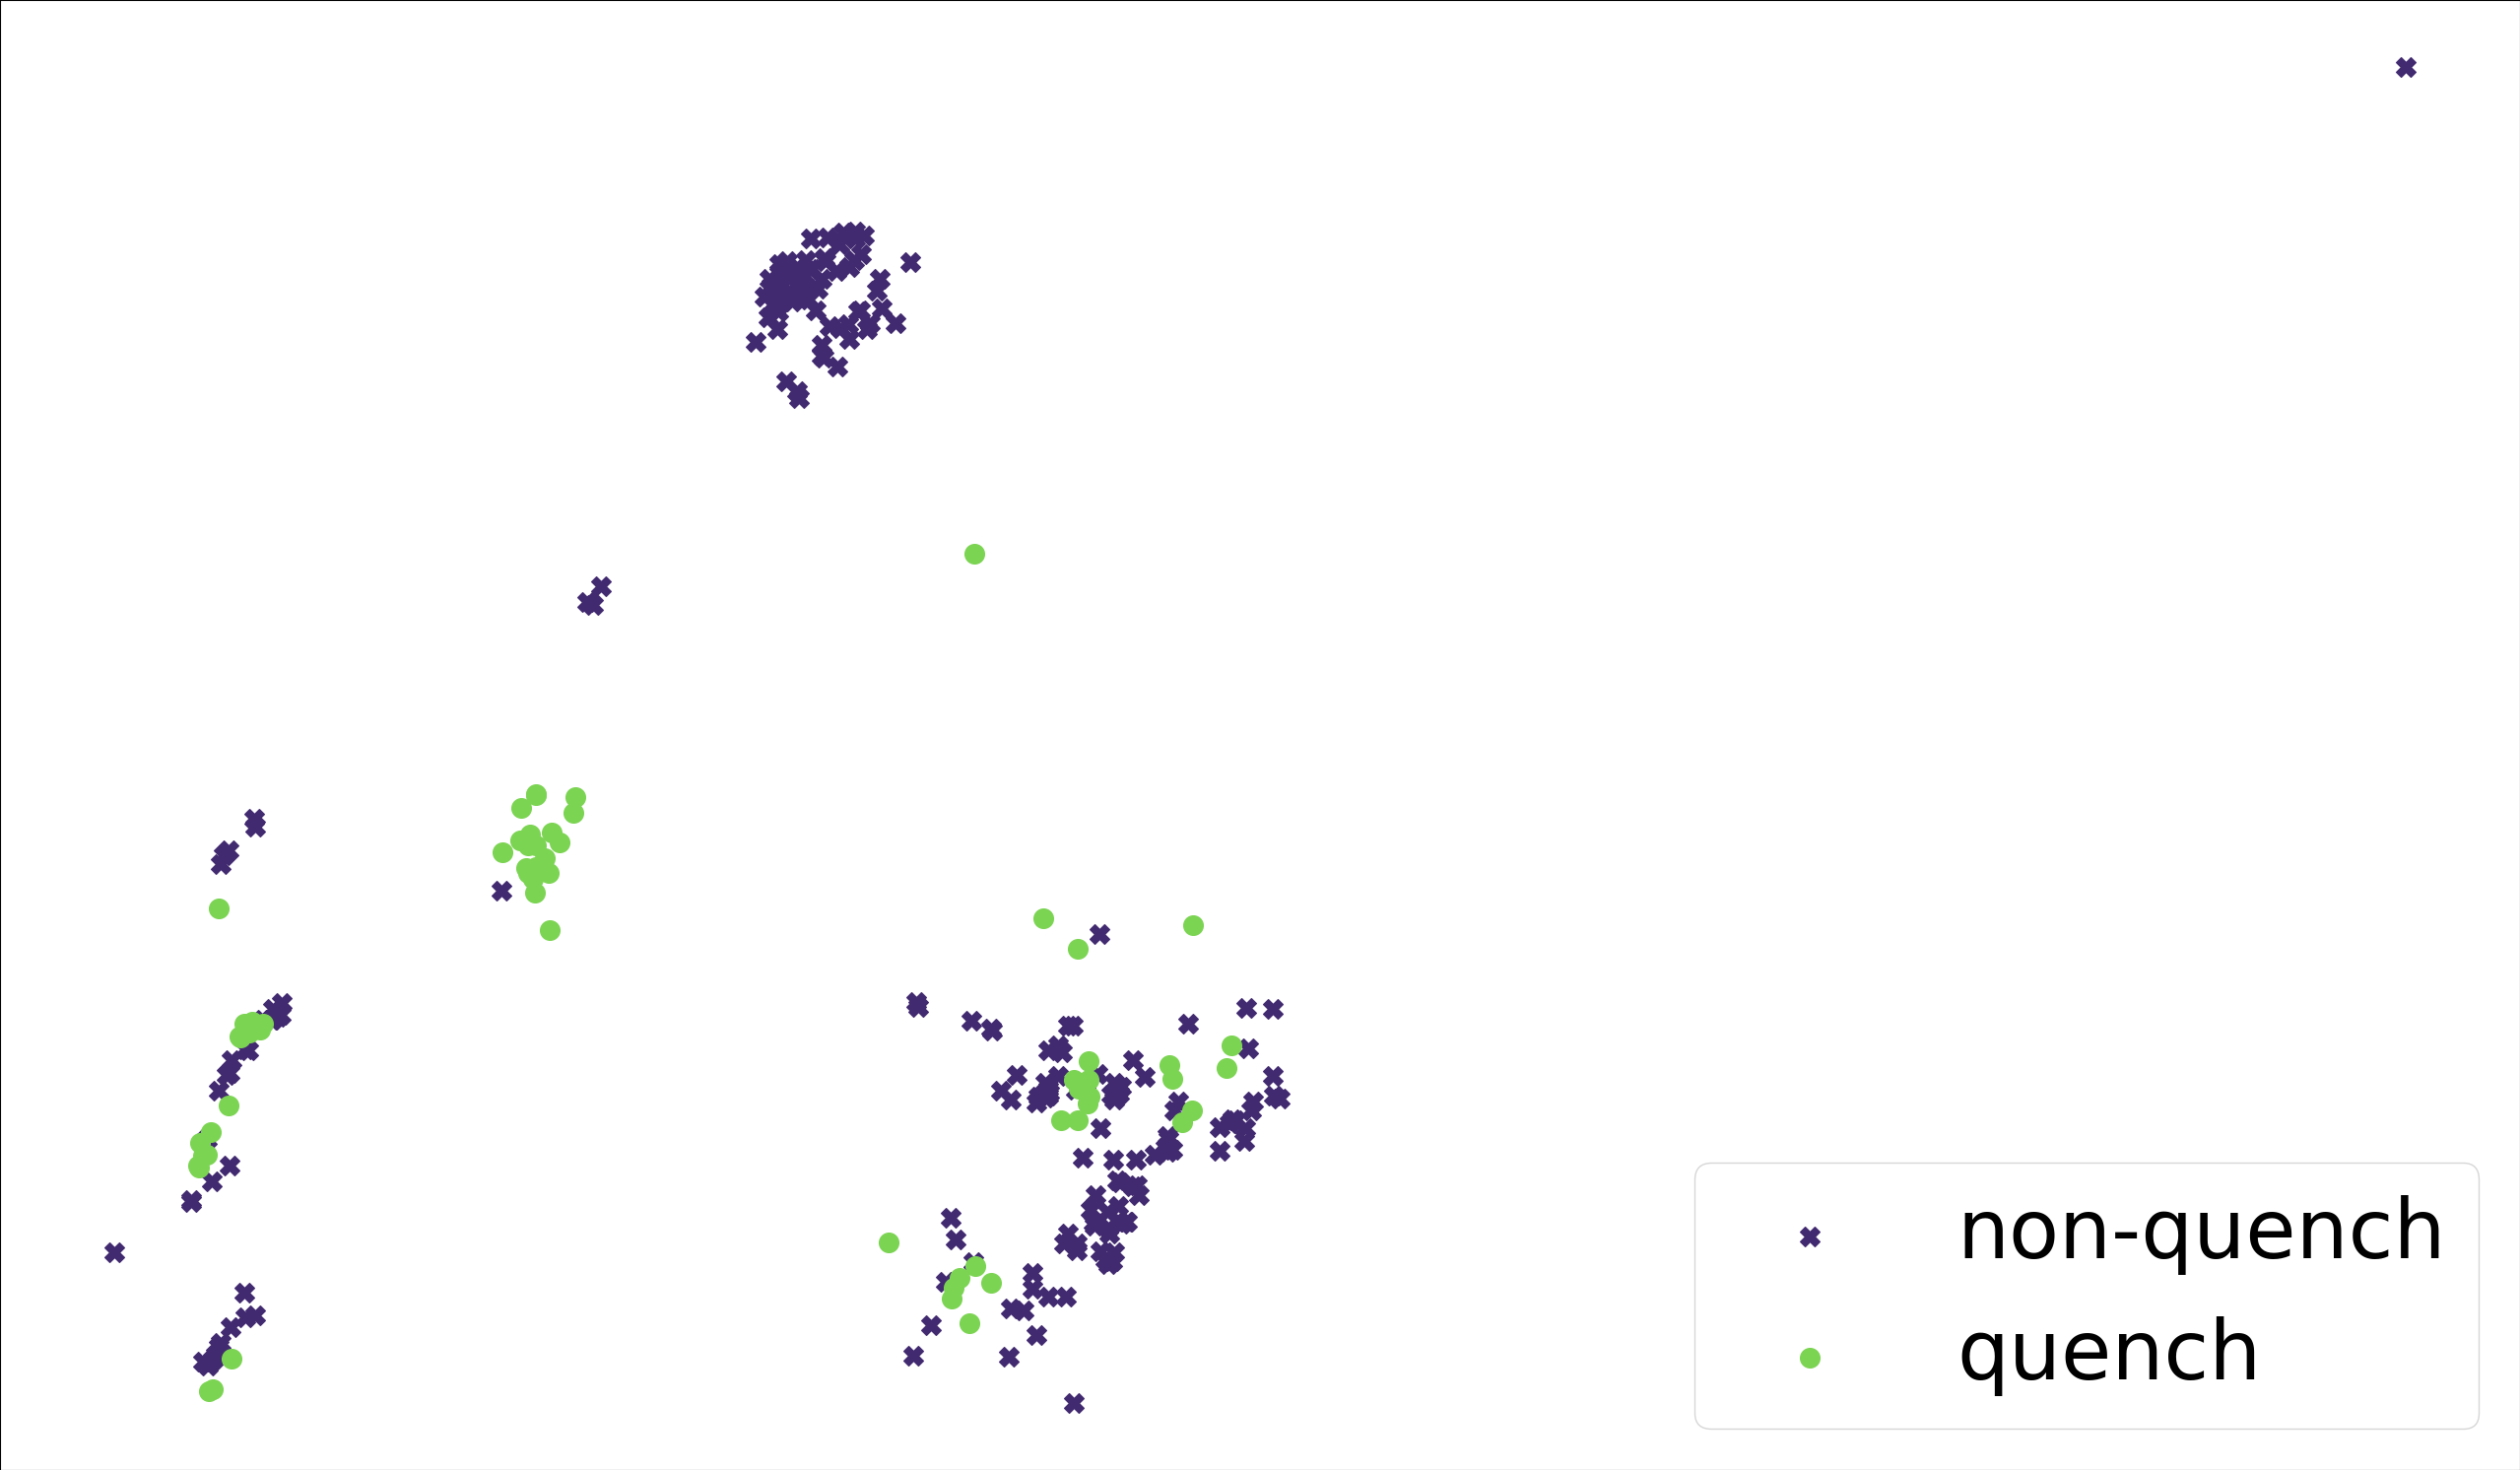
\includegraphics[width=\linewidth]{img/quench_dist_qlp/quenches_coil_0_Cnmod.png}
		\subcaption{}
	\end{subfigure}
	\begin{subfigure}{0.49\linewidth}
		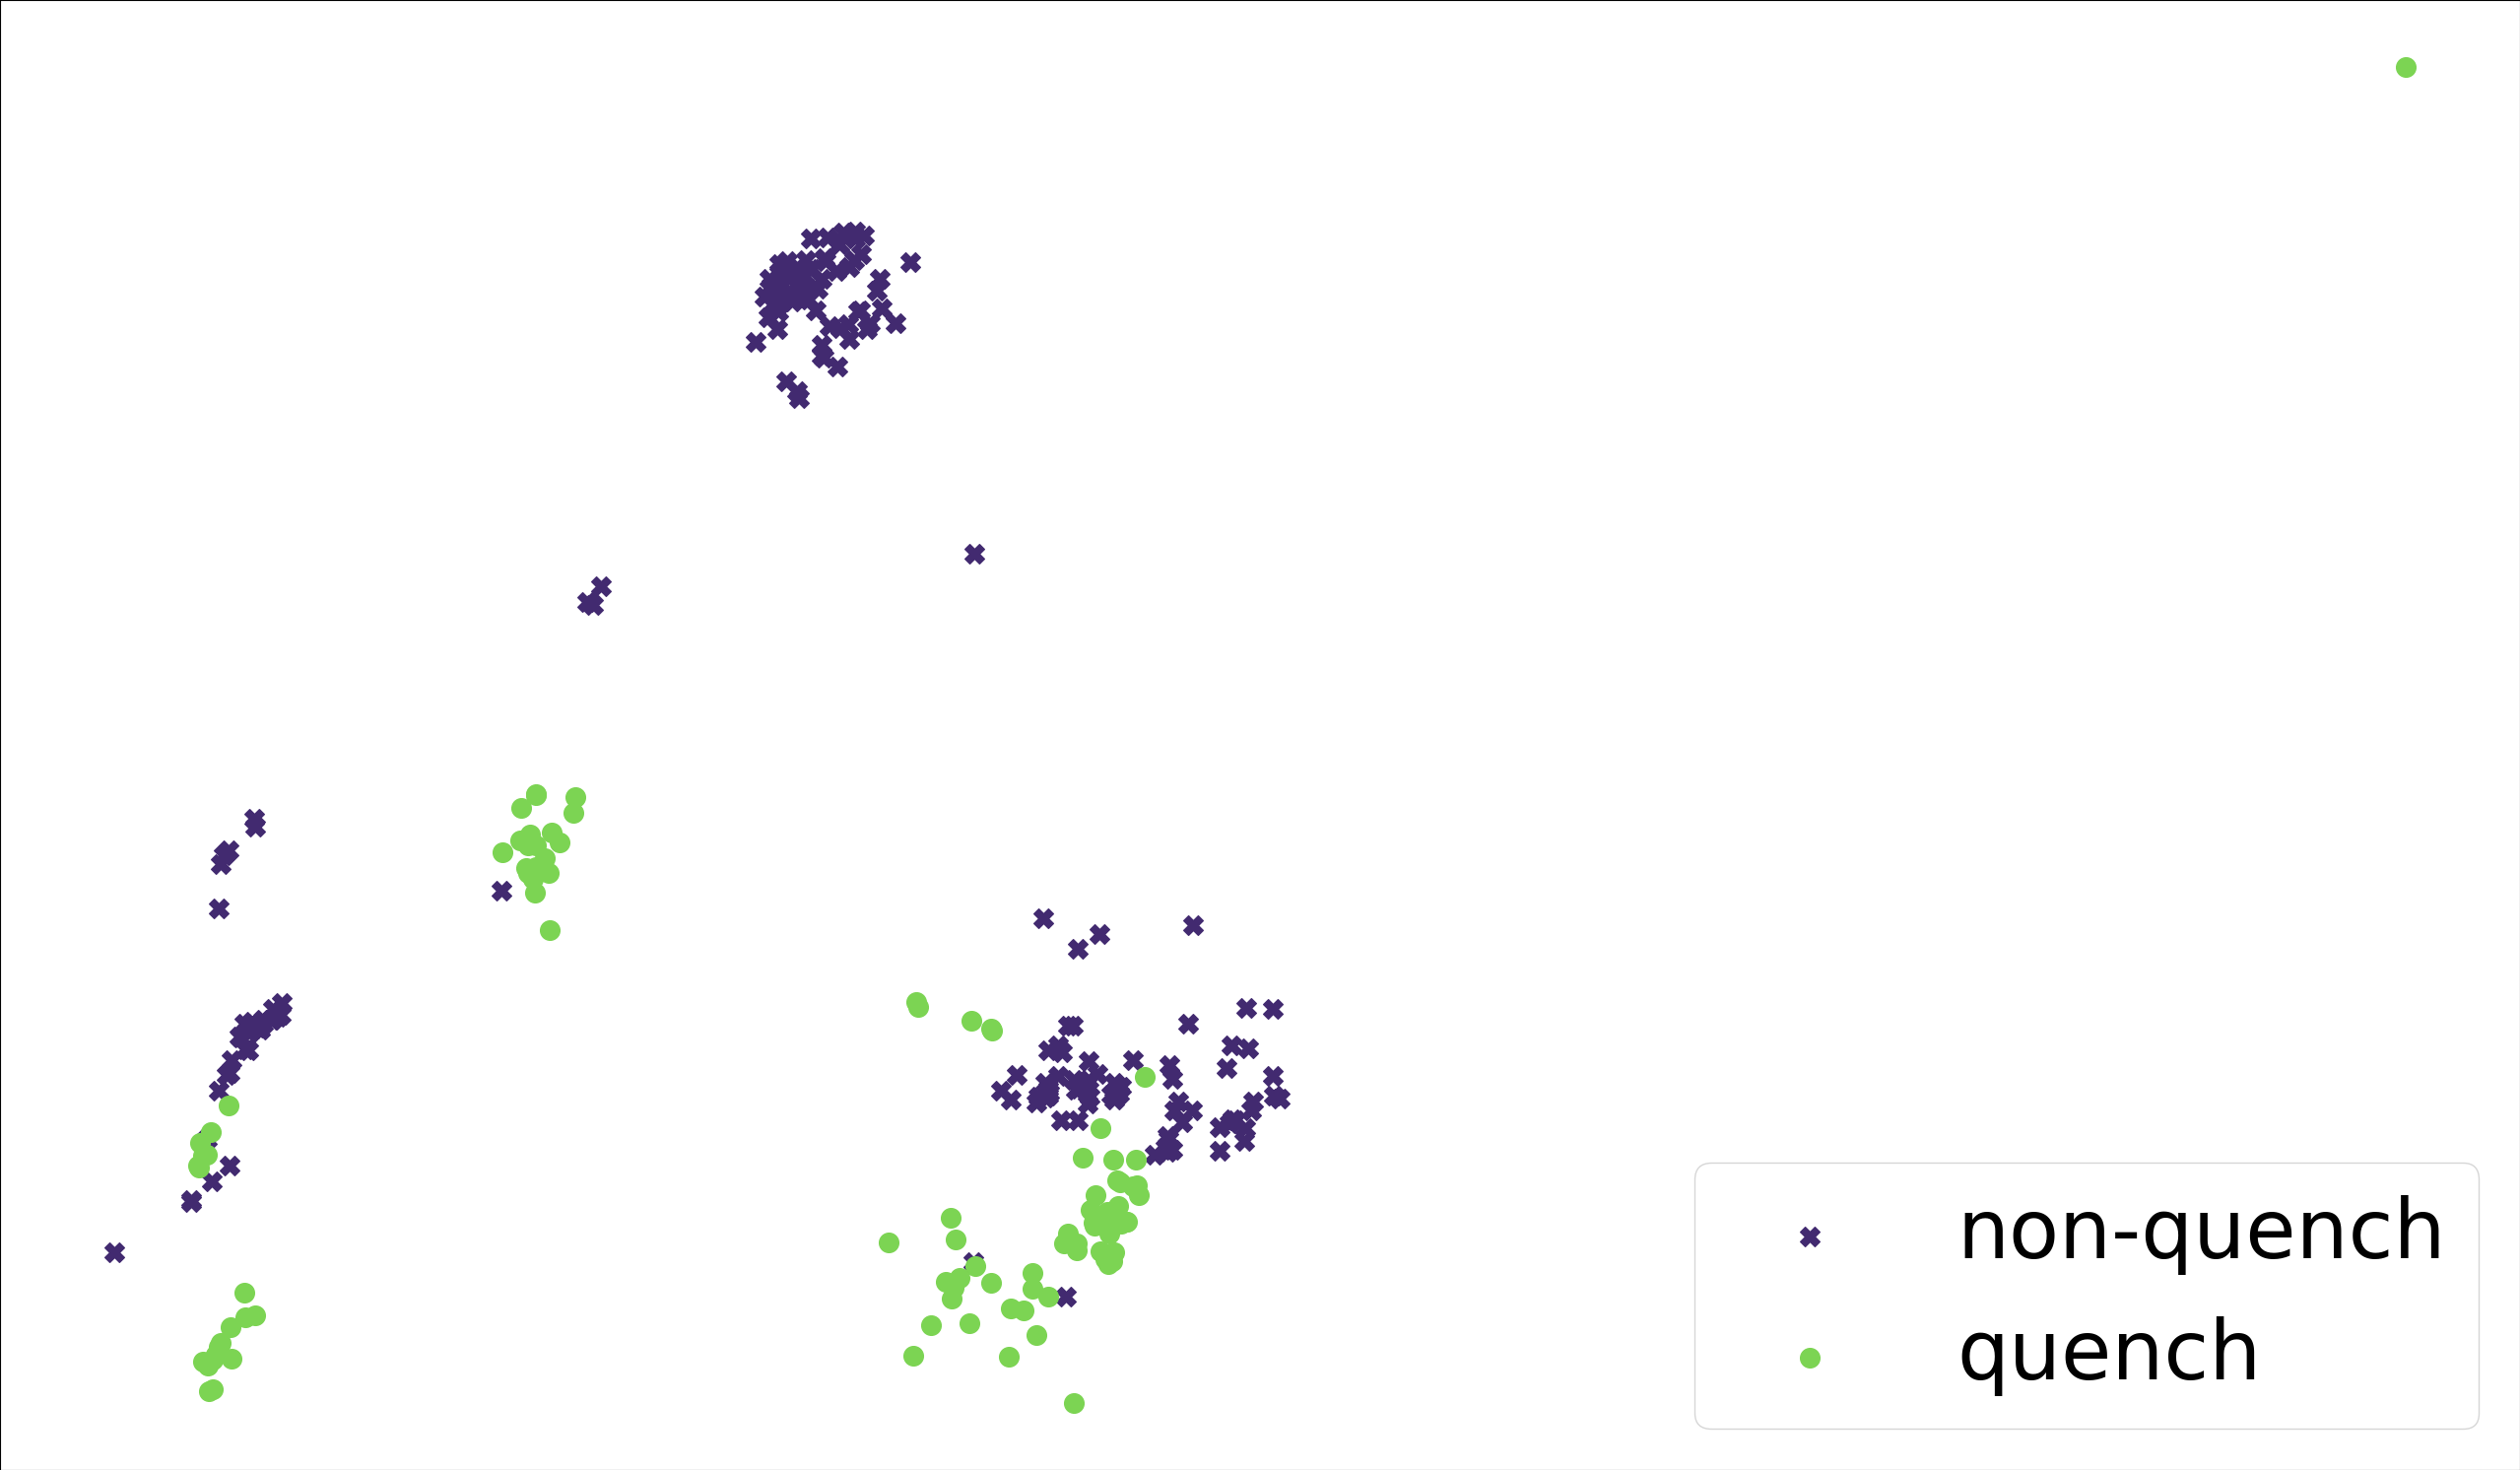
\includegraphics[width=\linewidth]{img/quench_dist_qlp/quenches_coil_1_Cnmod.png}
		\subcaption{}
	\end{subfigure}
	\begin{subfigure}{0.49\linewidth}
		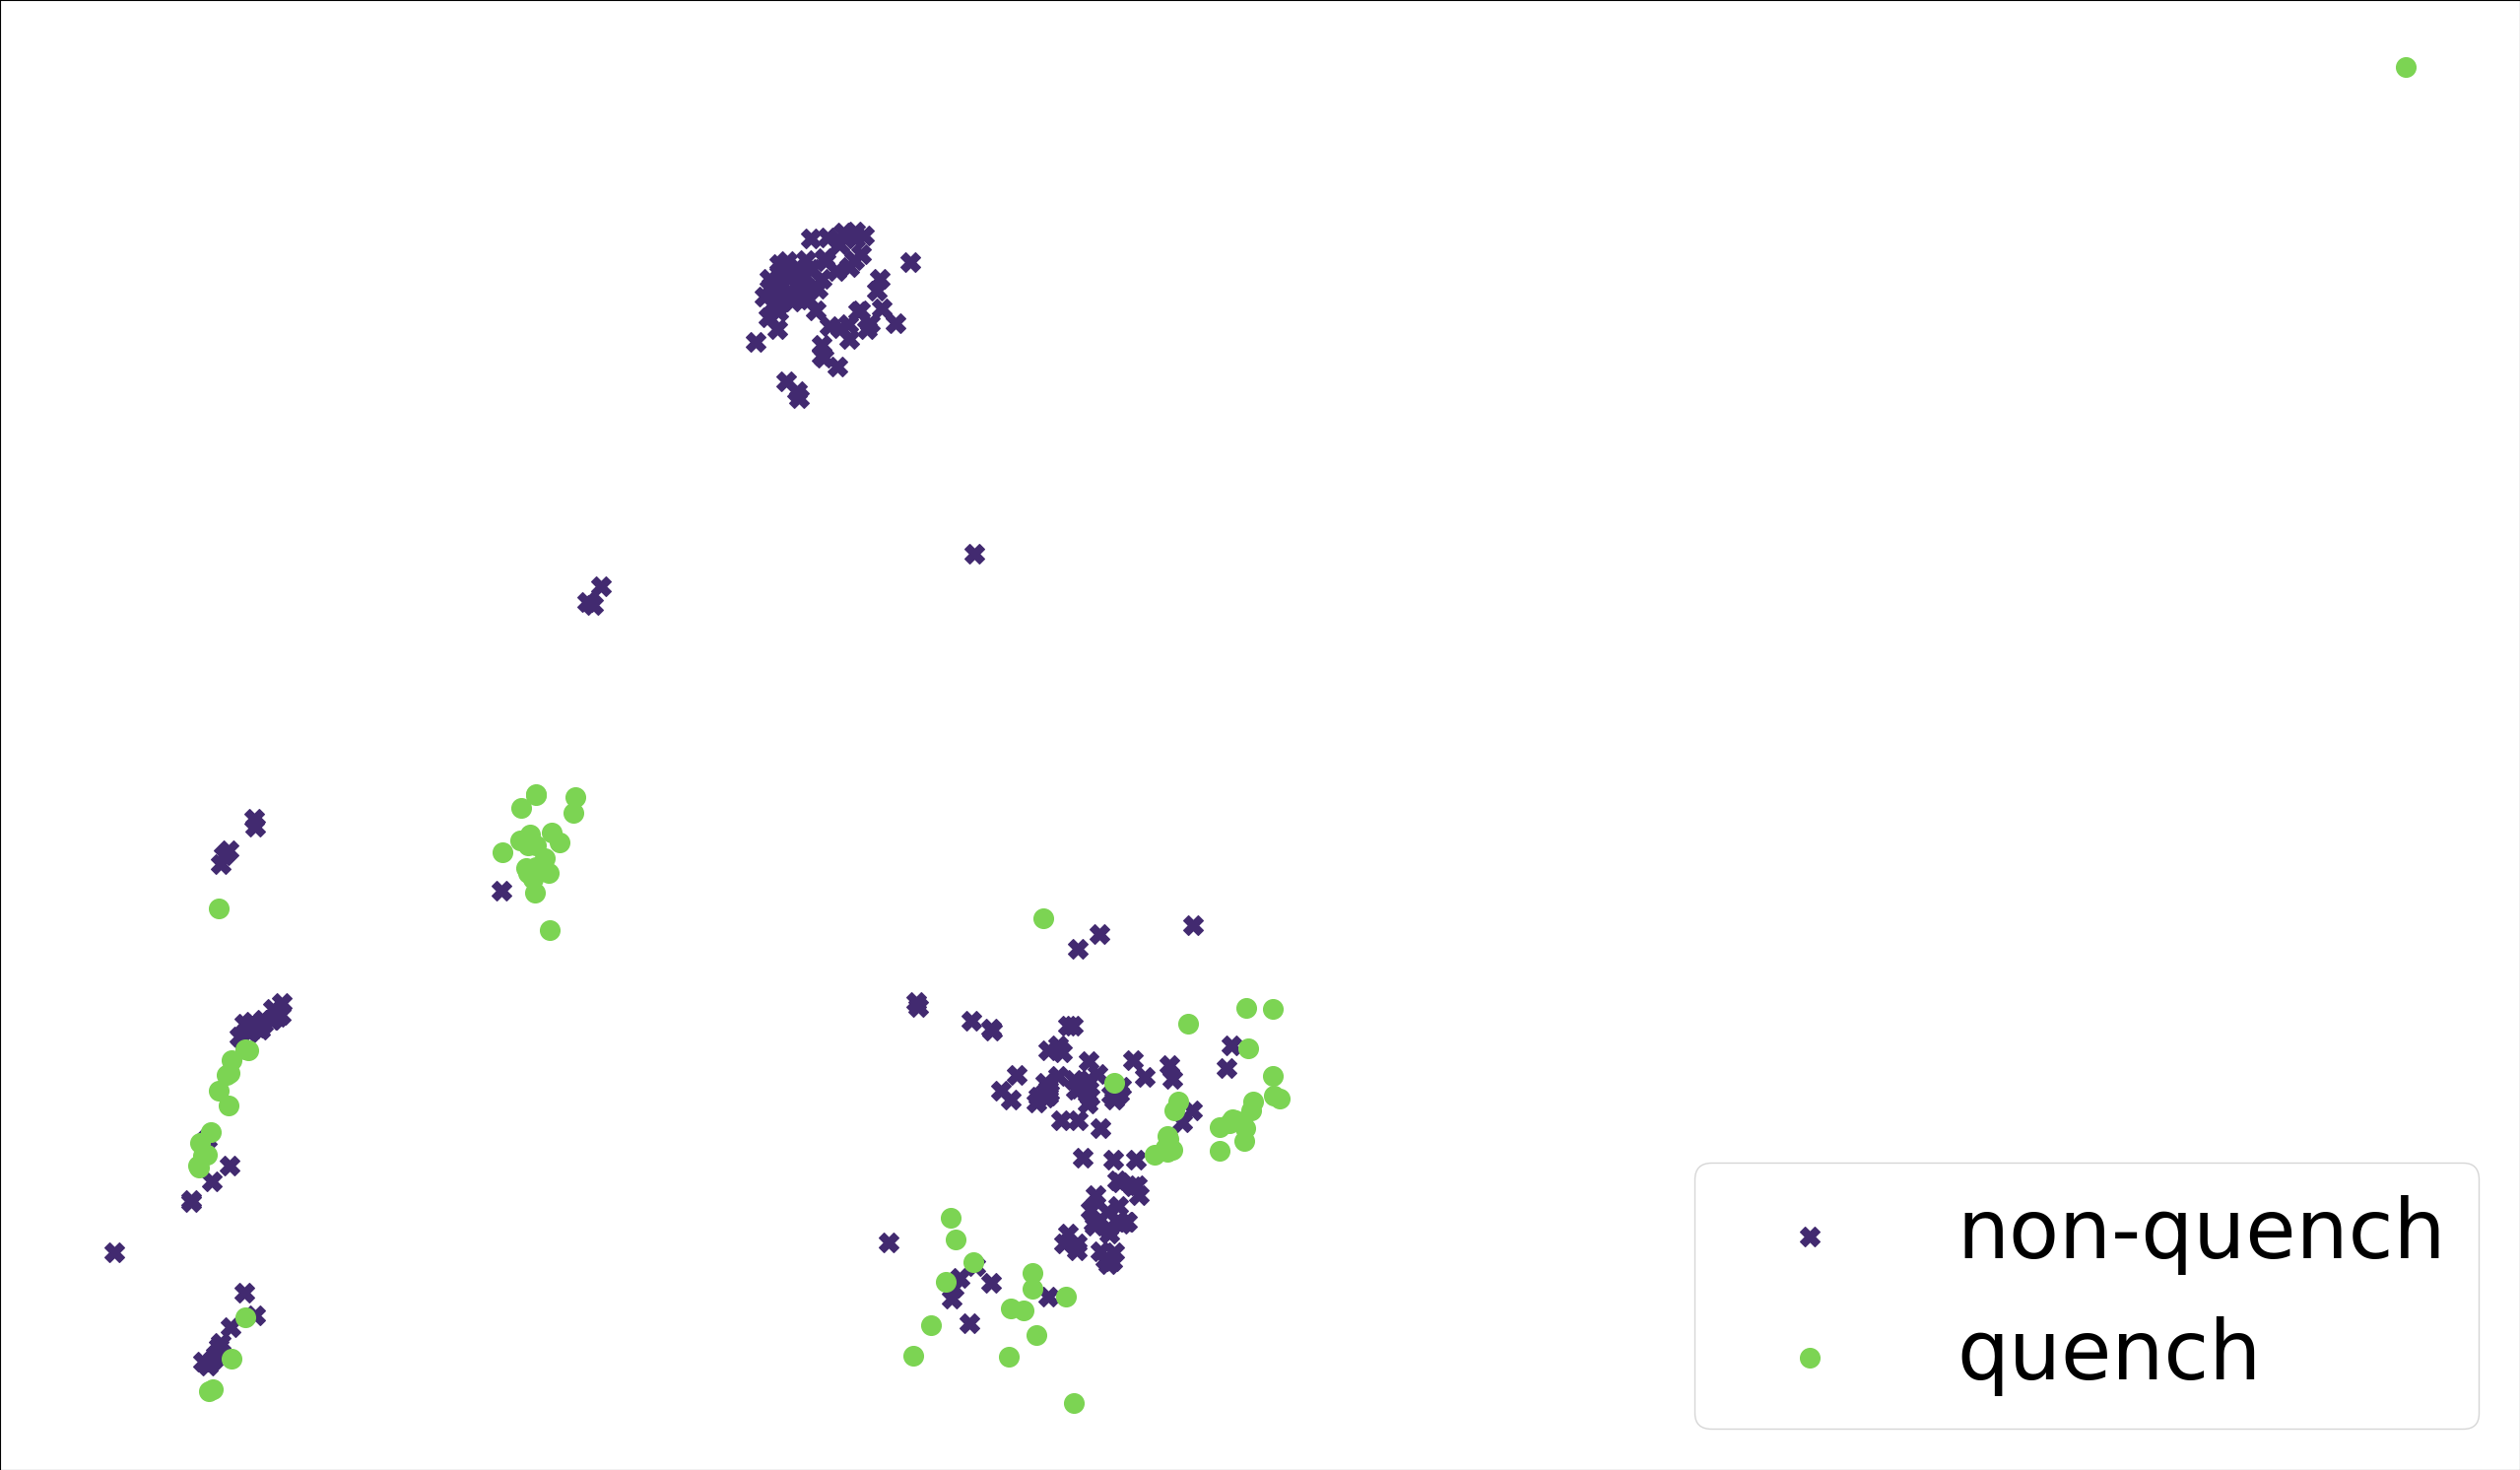
\includegraphics[width=\linewidth]{img/quench_dist_qlp/quenches_coil_2_Cnmod.png}
		\subcaption{}
	\end{subfigure}
	\begin{subfigure}{0.49\linewidth}
		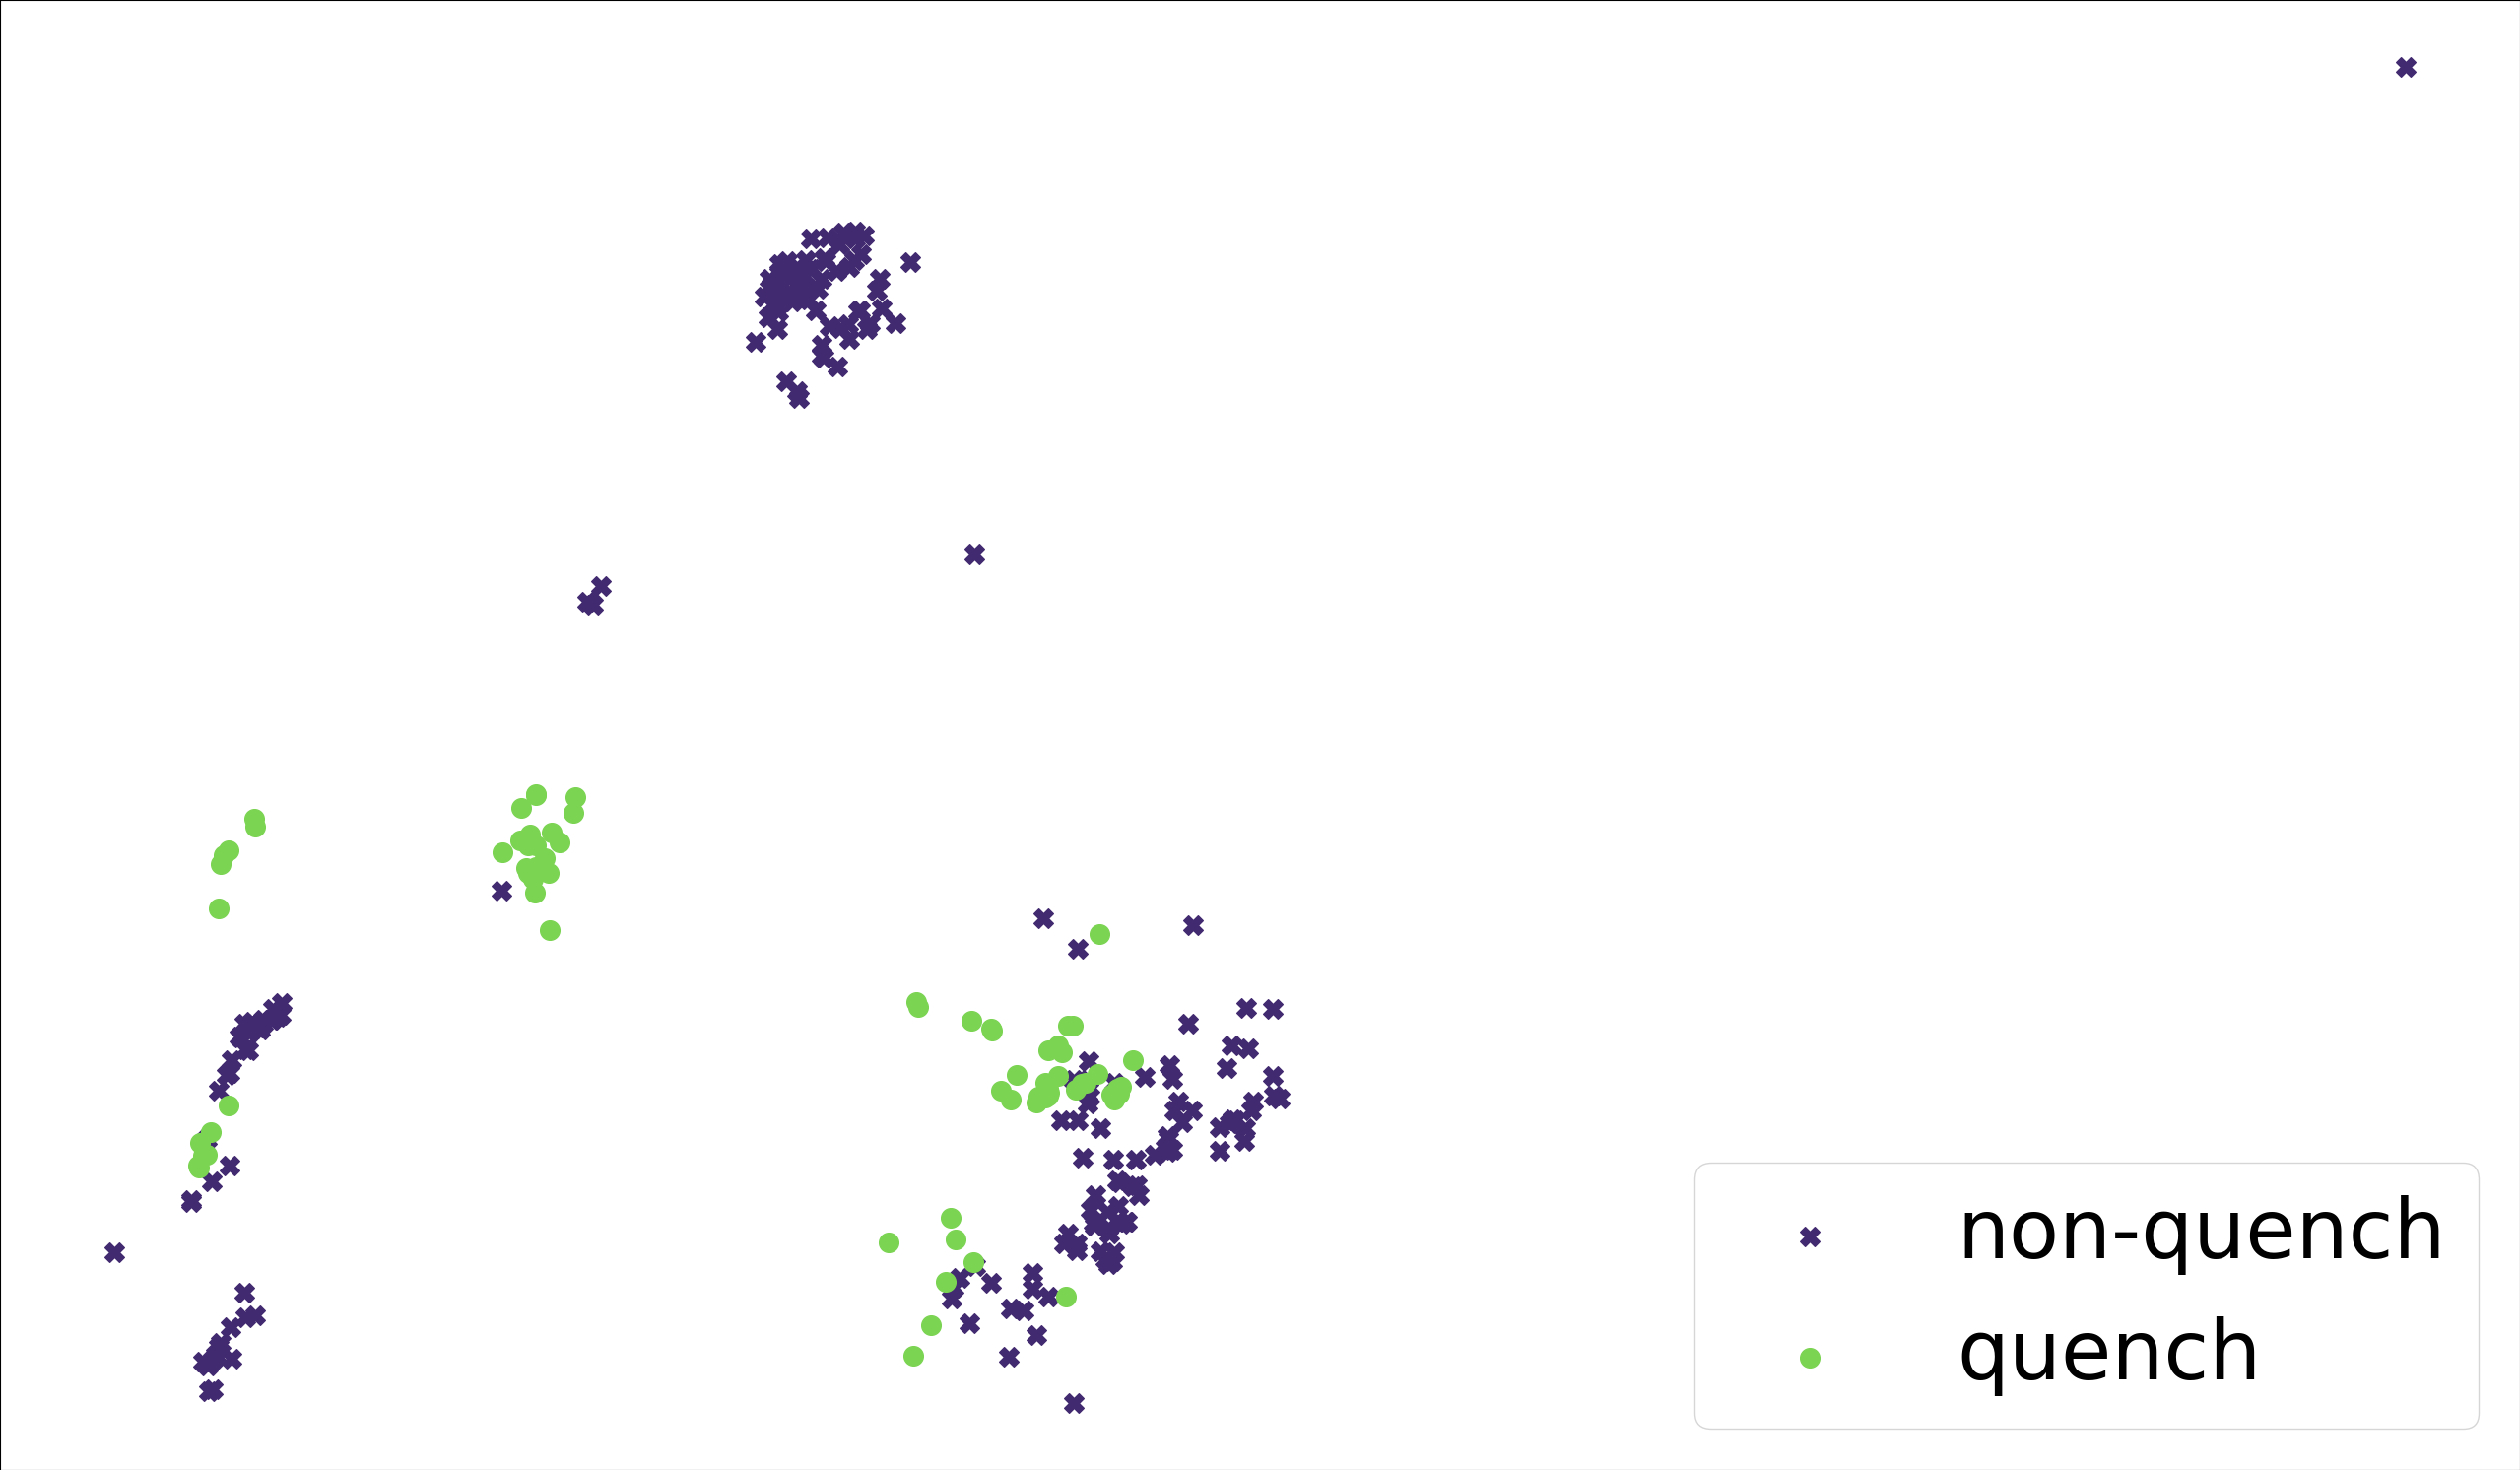
\includegraphics[width=\linewidth]{img/quench_dist_qlp/quenches_coil_3_Cnmod.png}
		\subcaption{}
	\end{subfigure}
	\caption{The distribution of the samples in bidimensional space after a round of \pca, for
		the \cnmod\ attribute. the subfigures contain different views of the same data: (a) differenciates between non-quench and single or multiple quench events, (b) highlights the distribution of quenches for coil $0$, (c) highlights the distribution of quenches for coil $1$, (d) highlights the distribution of quenches for coil $2$ and finally (e) highlights the distribution of quenches for coil $3$.}
	\label{fig:cnmod-coilq-dist}
\end{figure}

\subsubsection{\phin}
To close this subsection about the preprocessing step we can consider the \phin\ dataset, which
seems to be highly informative across the board, and due to the lack of strong correlation between
the harmonics (as testified in the preprocessing step done for \qrp), we could probably use it for
all coils and still get good performance. Probably the best sub-view for \phin is going to contain
all of the harmonics with the exception of: only one harmonic from \{\phin[2], \phin[6], \phin[10],
\phin[14]\}, and only one harmonic from \{\phin[4], \phin[8], \phin[12]\}.

\begin{figure}[!h]
	% Font size = 70
	\centering
	\begin{subfigure}{0.49\linewidth}
		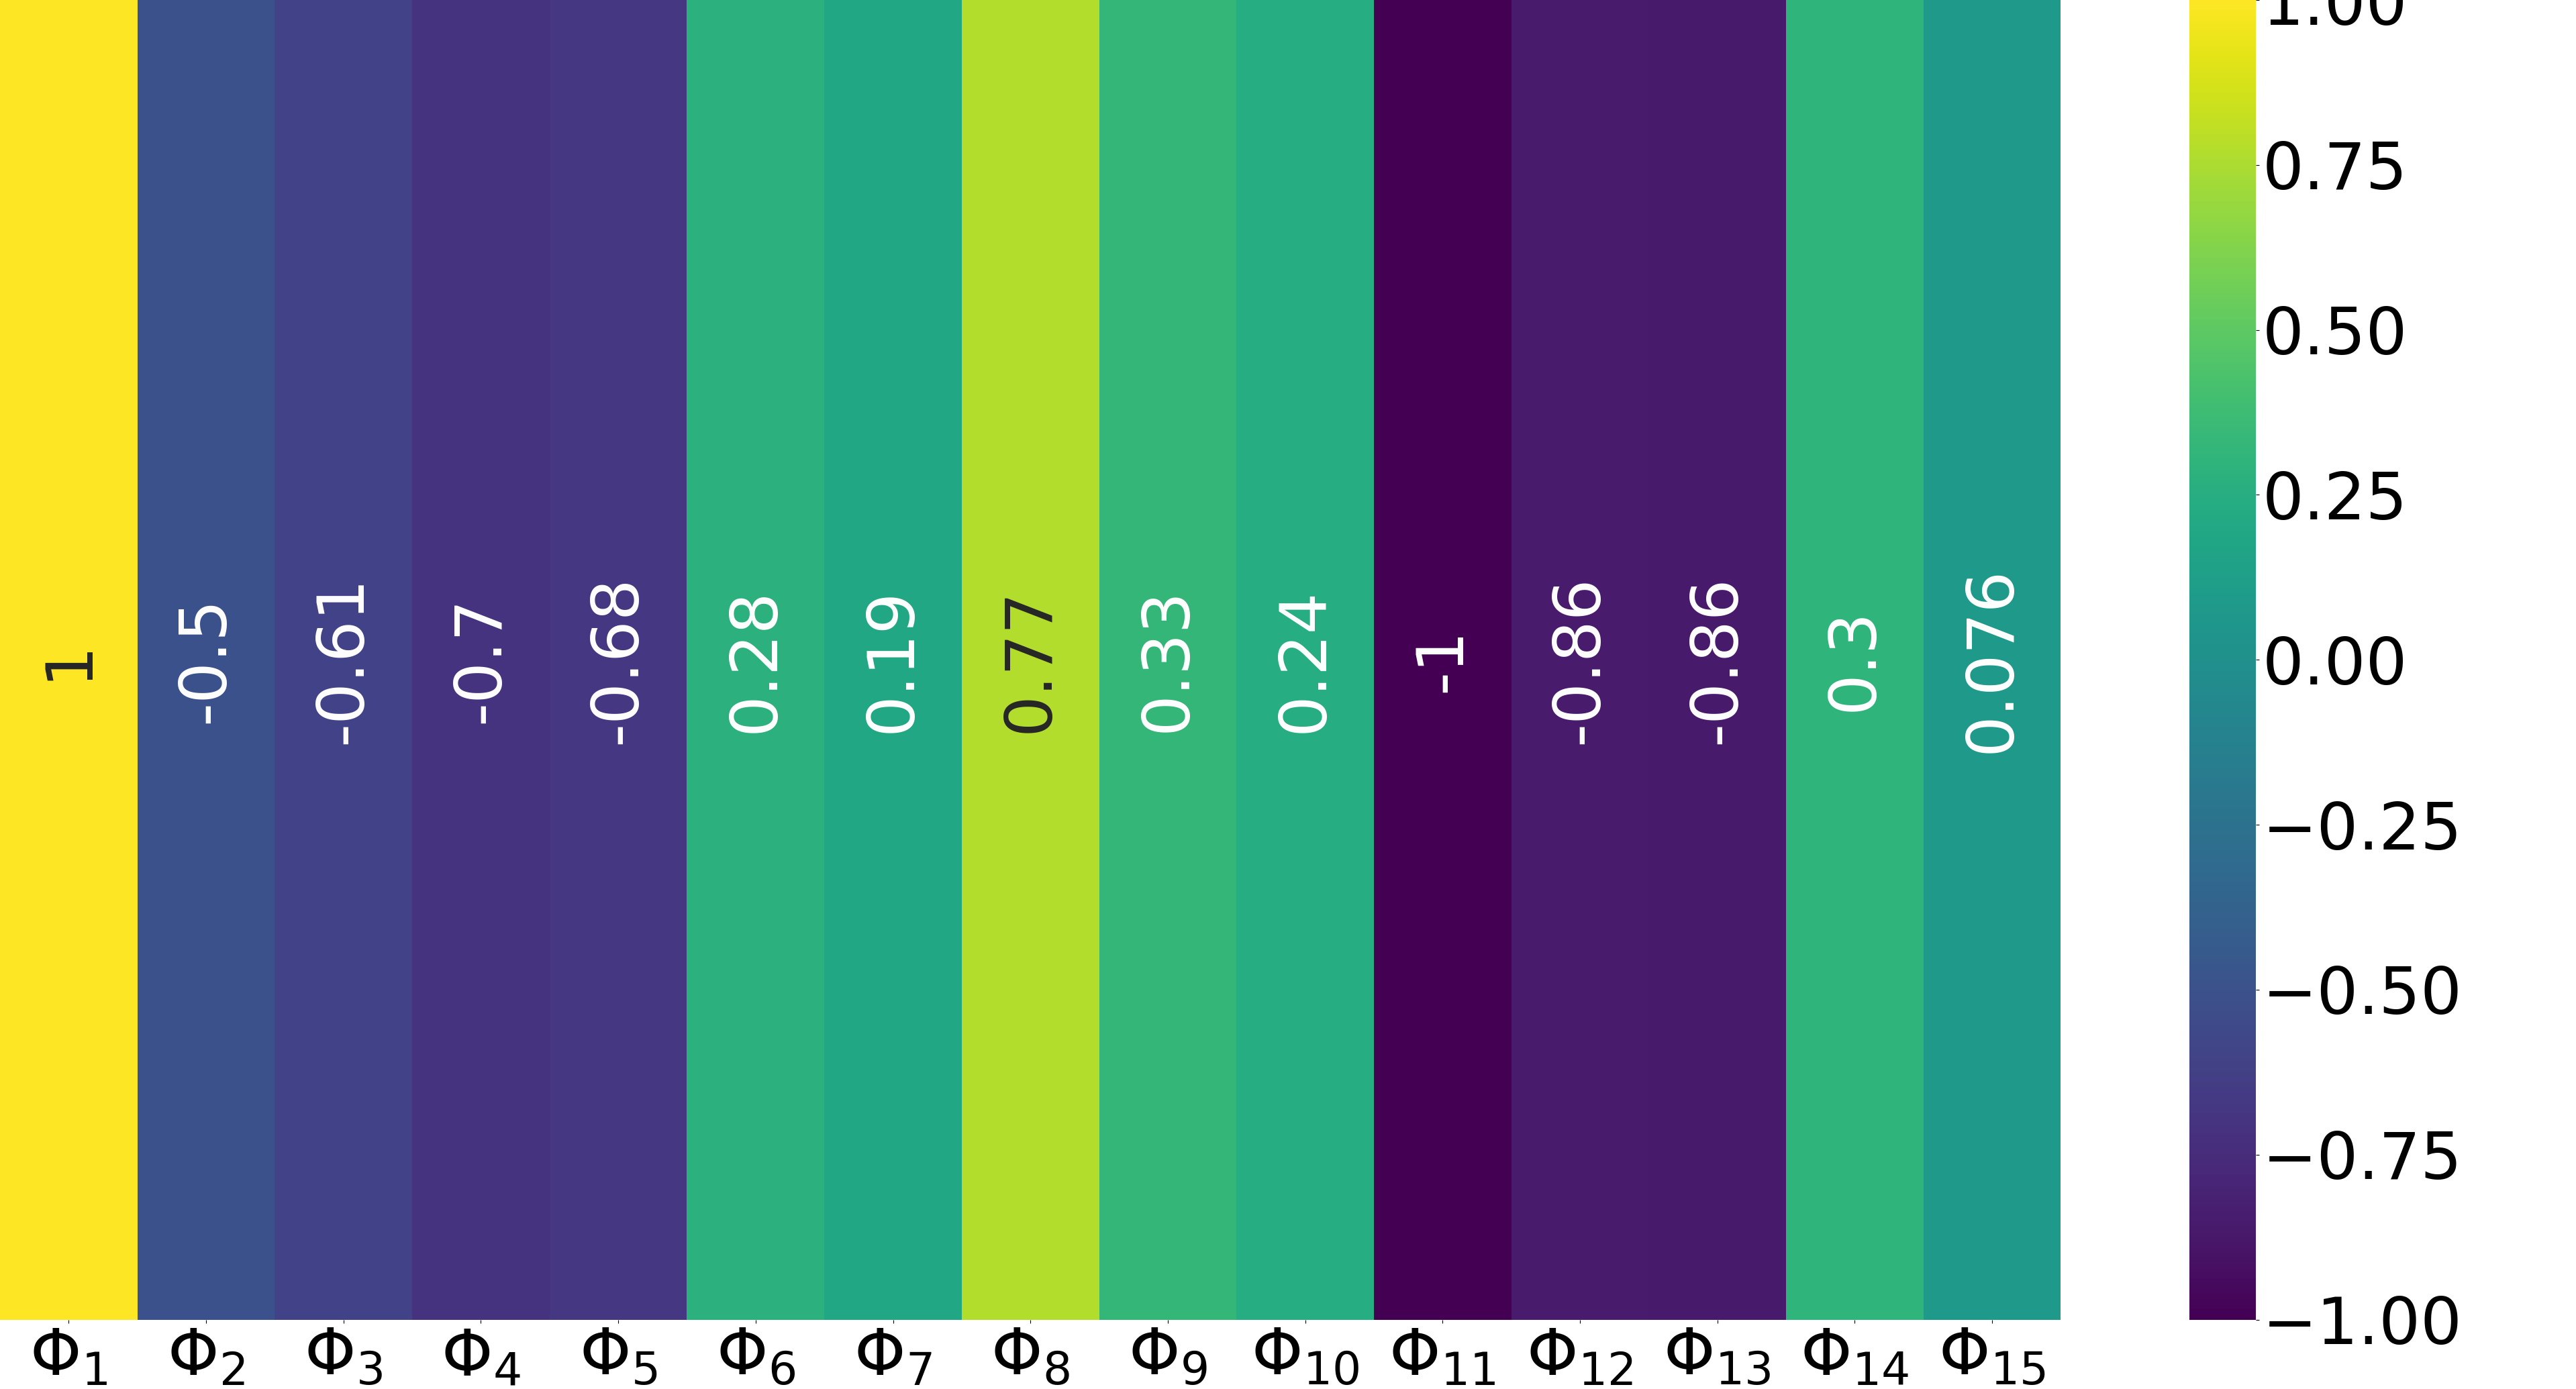
\includegraphics[width=\linewidth]{img/qlp_corr/Phi_coil0.png}
		\subcaption{Correlation with coil $0$}
	\end{subfigure}
	\begin{subfigure}{0.49\linewidth}
		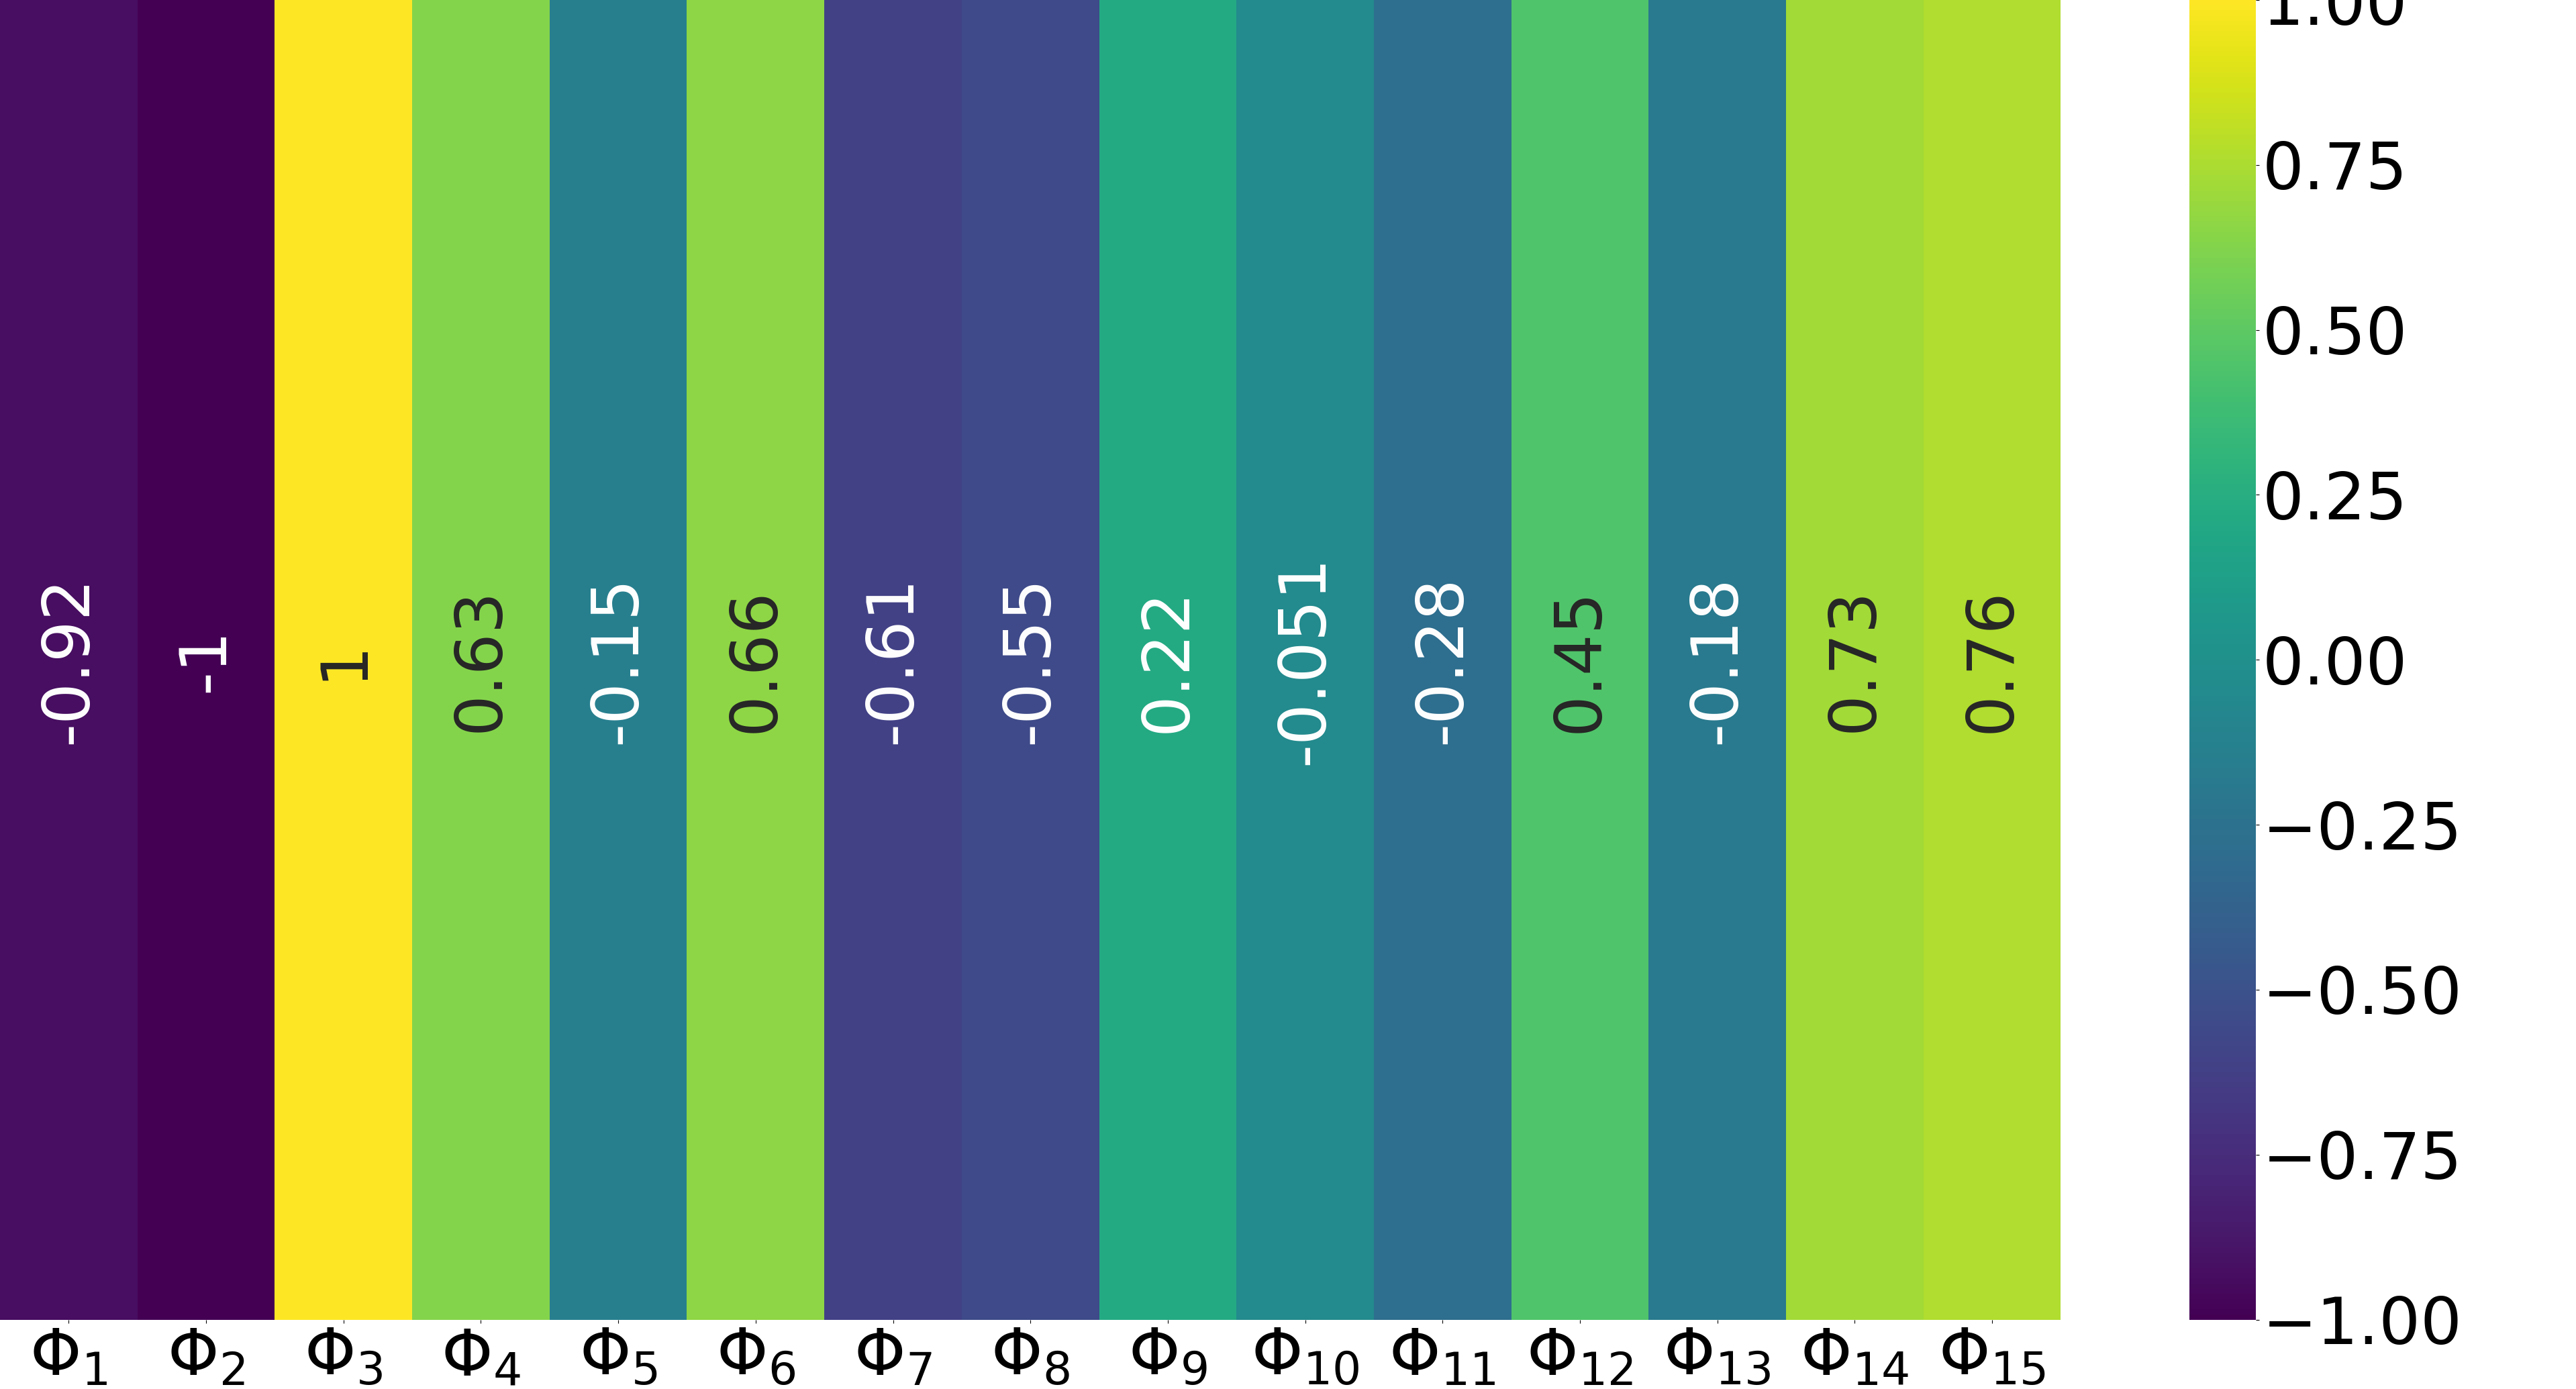
\includegraphics[width=\linewidth]{img/qlp_corr/Phi_coil1.png}
		\subcaption{Correlation with coil $1$}
	\end{subfigure}
	\begin{subfigure}{0.49\linewidth}
		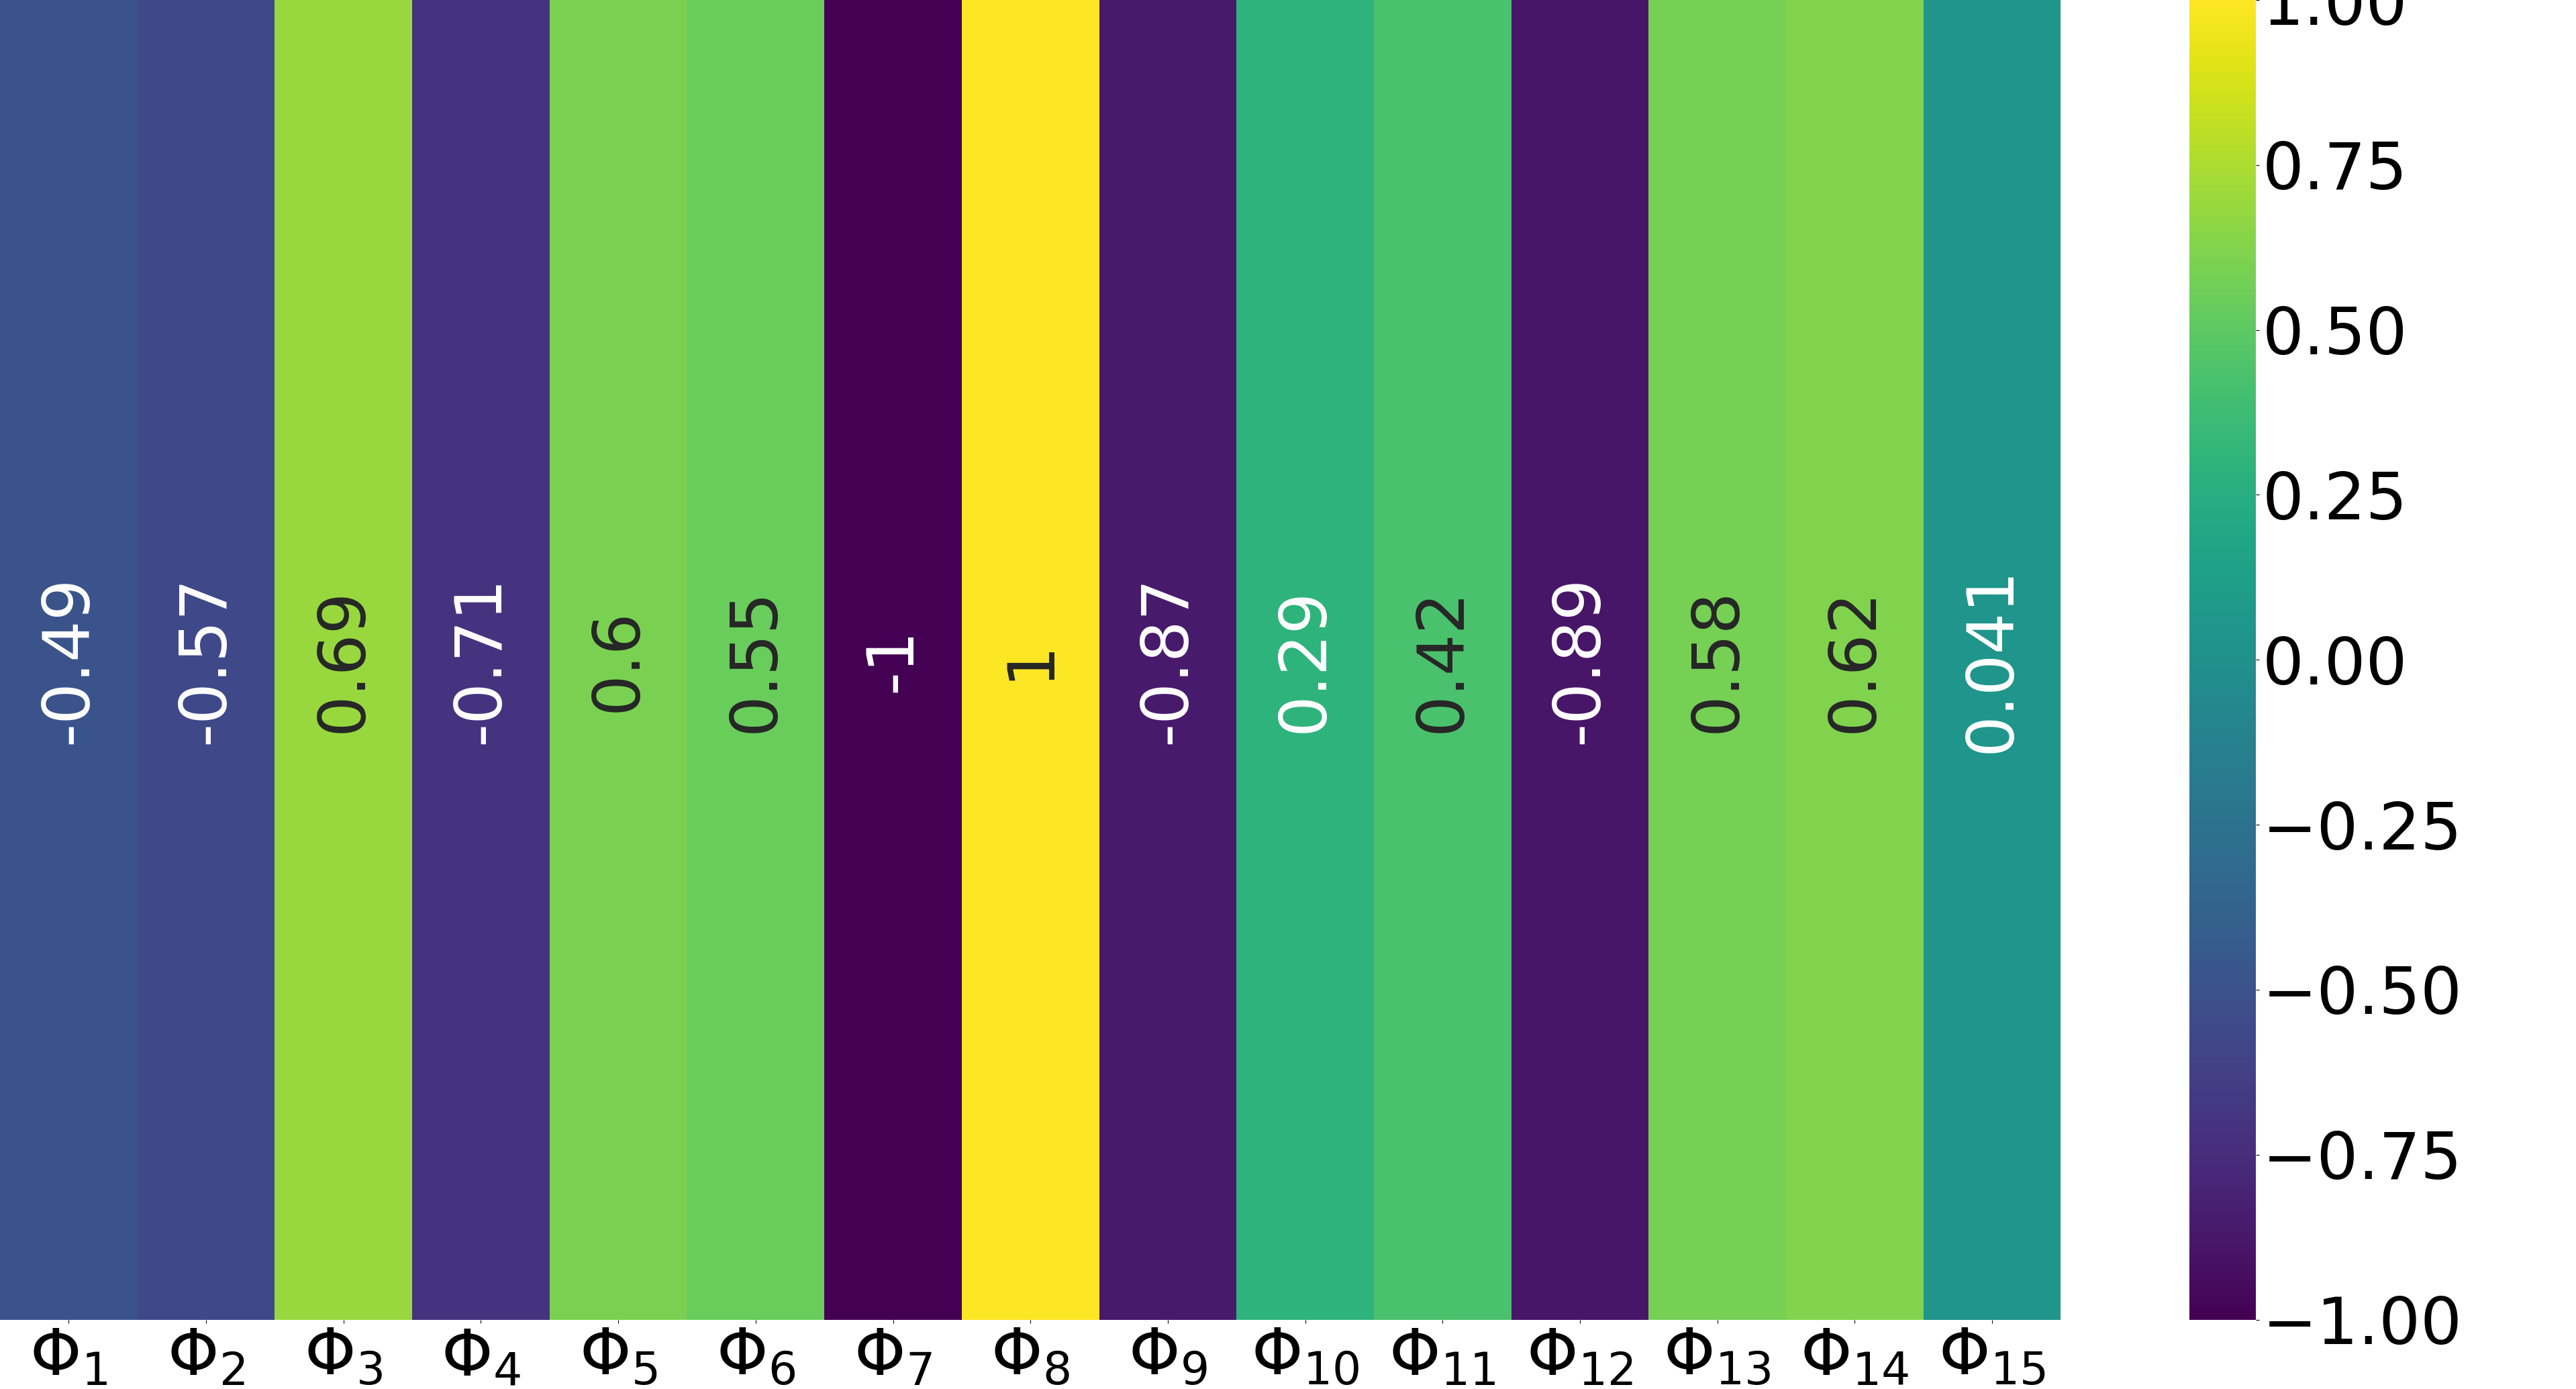
\includegraphics[width=\linewidth]{img/qlp_corr/Phi_coil2.png}
		\subcaption{Correlation with coil $2$}
	\end{subfigure}
	\begin{subfigure}{0.49\linewidth}
		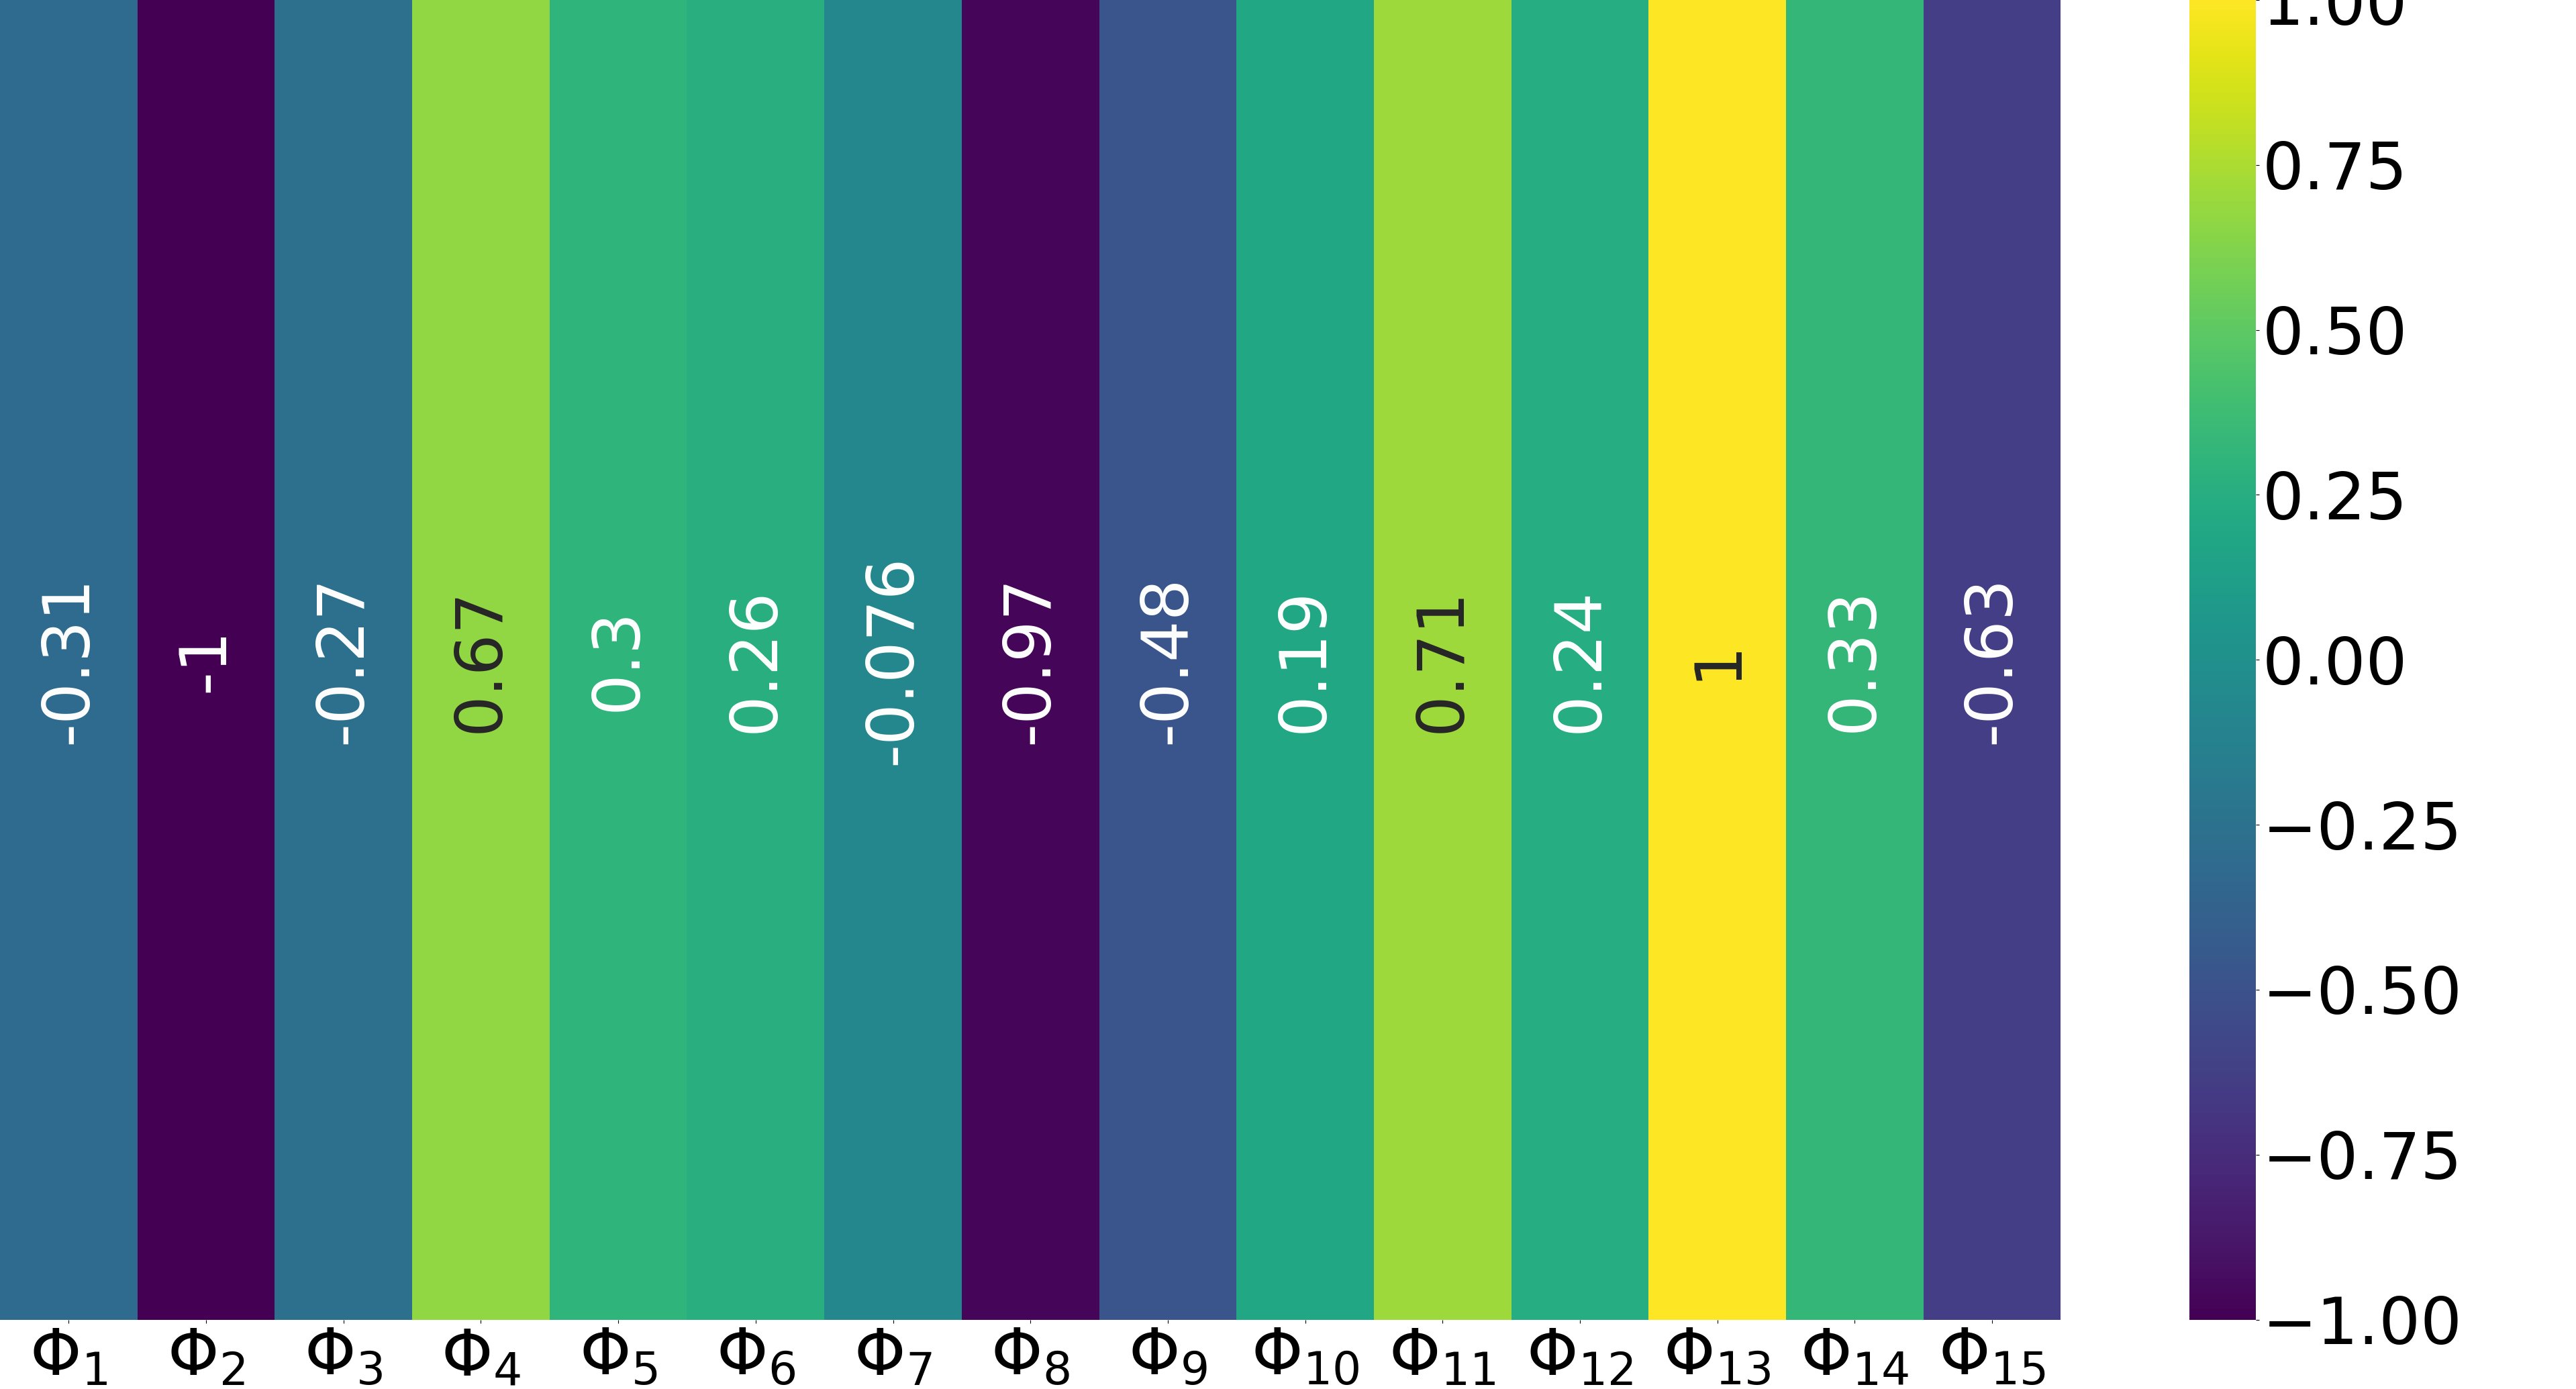
\includegraphics[width=\linewidth]{img/qlp_corr/Phi_coil3.png}
		\subcaption{Correlation with coil $3$}
	\end{subfigure}
	\caption{Correlation between the harmonics of the \phin\ attribute and the labels for \qlp.}
	\label{fig:phi-lcorr-qlp}
\end{figure}

As we have done so far, we visualize the distribution of the data after moving from $15$ to $2$
dimensions using \pca (see \Cref{fig:phi-coilq-dist}), the result is that, apart from the cluster to
the left in sub-figure (a), which mostly contains non-quench events, the cluster on the right has a
high degree of homogeneity. The same conclusions apply to the analysis of quench localization for
the various coils, apart from specific cases, quenches have a bad distribution and are homogeneously
mixed to non-quench events in high impurity clusters.

\begin{figure}[!h]
	% Font size = 70
	\centering
	\begin{subfigure}{\linewidth}
		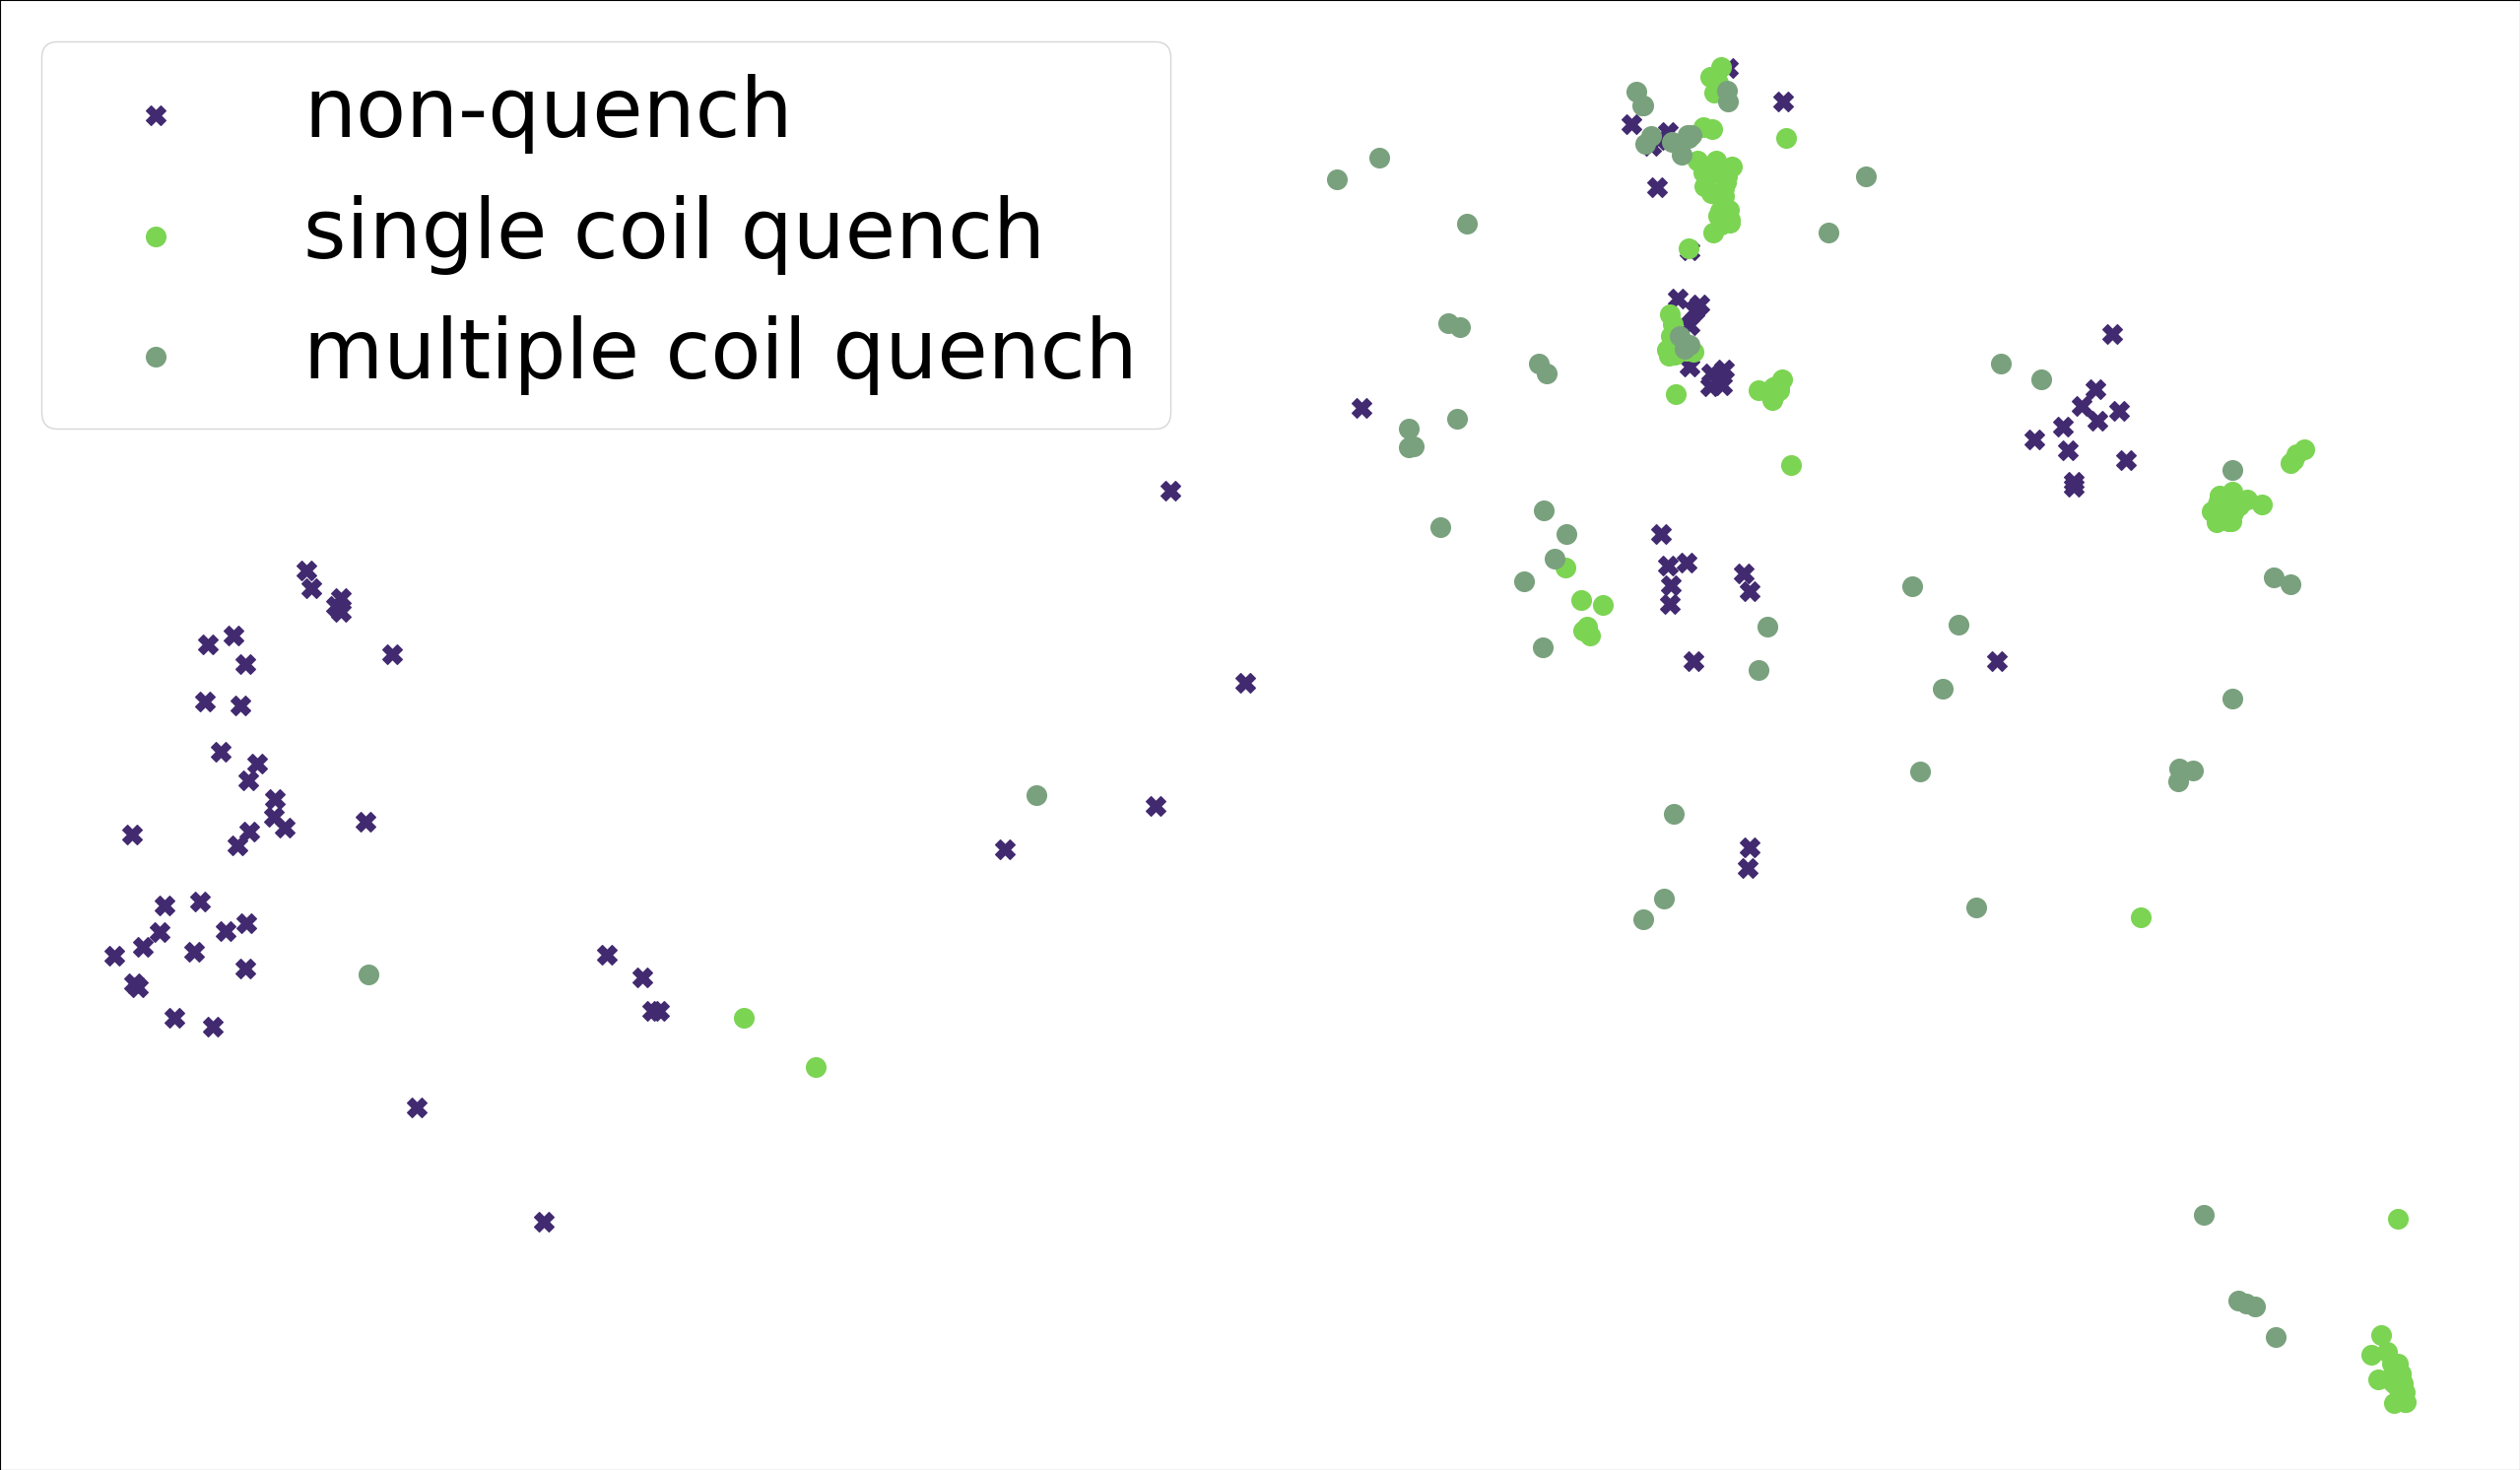
\includegraphics[width=\linewidth]{img/quench_dist_qlp/single_vs_multiple_Phi.png}
		\subcaption{}
	\end{subfigure}
	\begin{subfigure}{0.49\linewidth}
		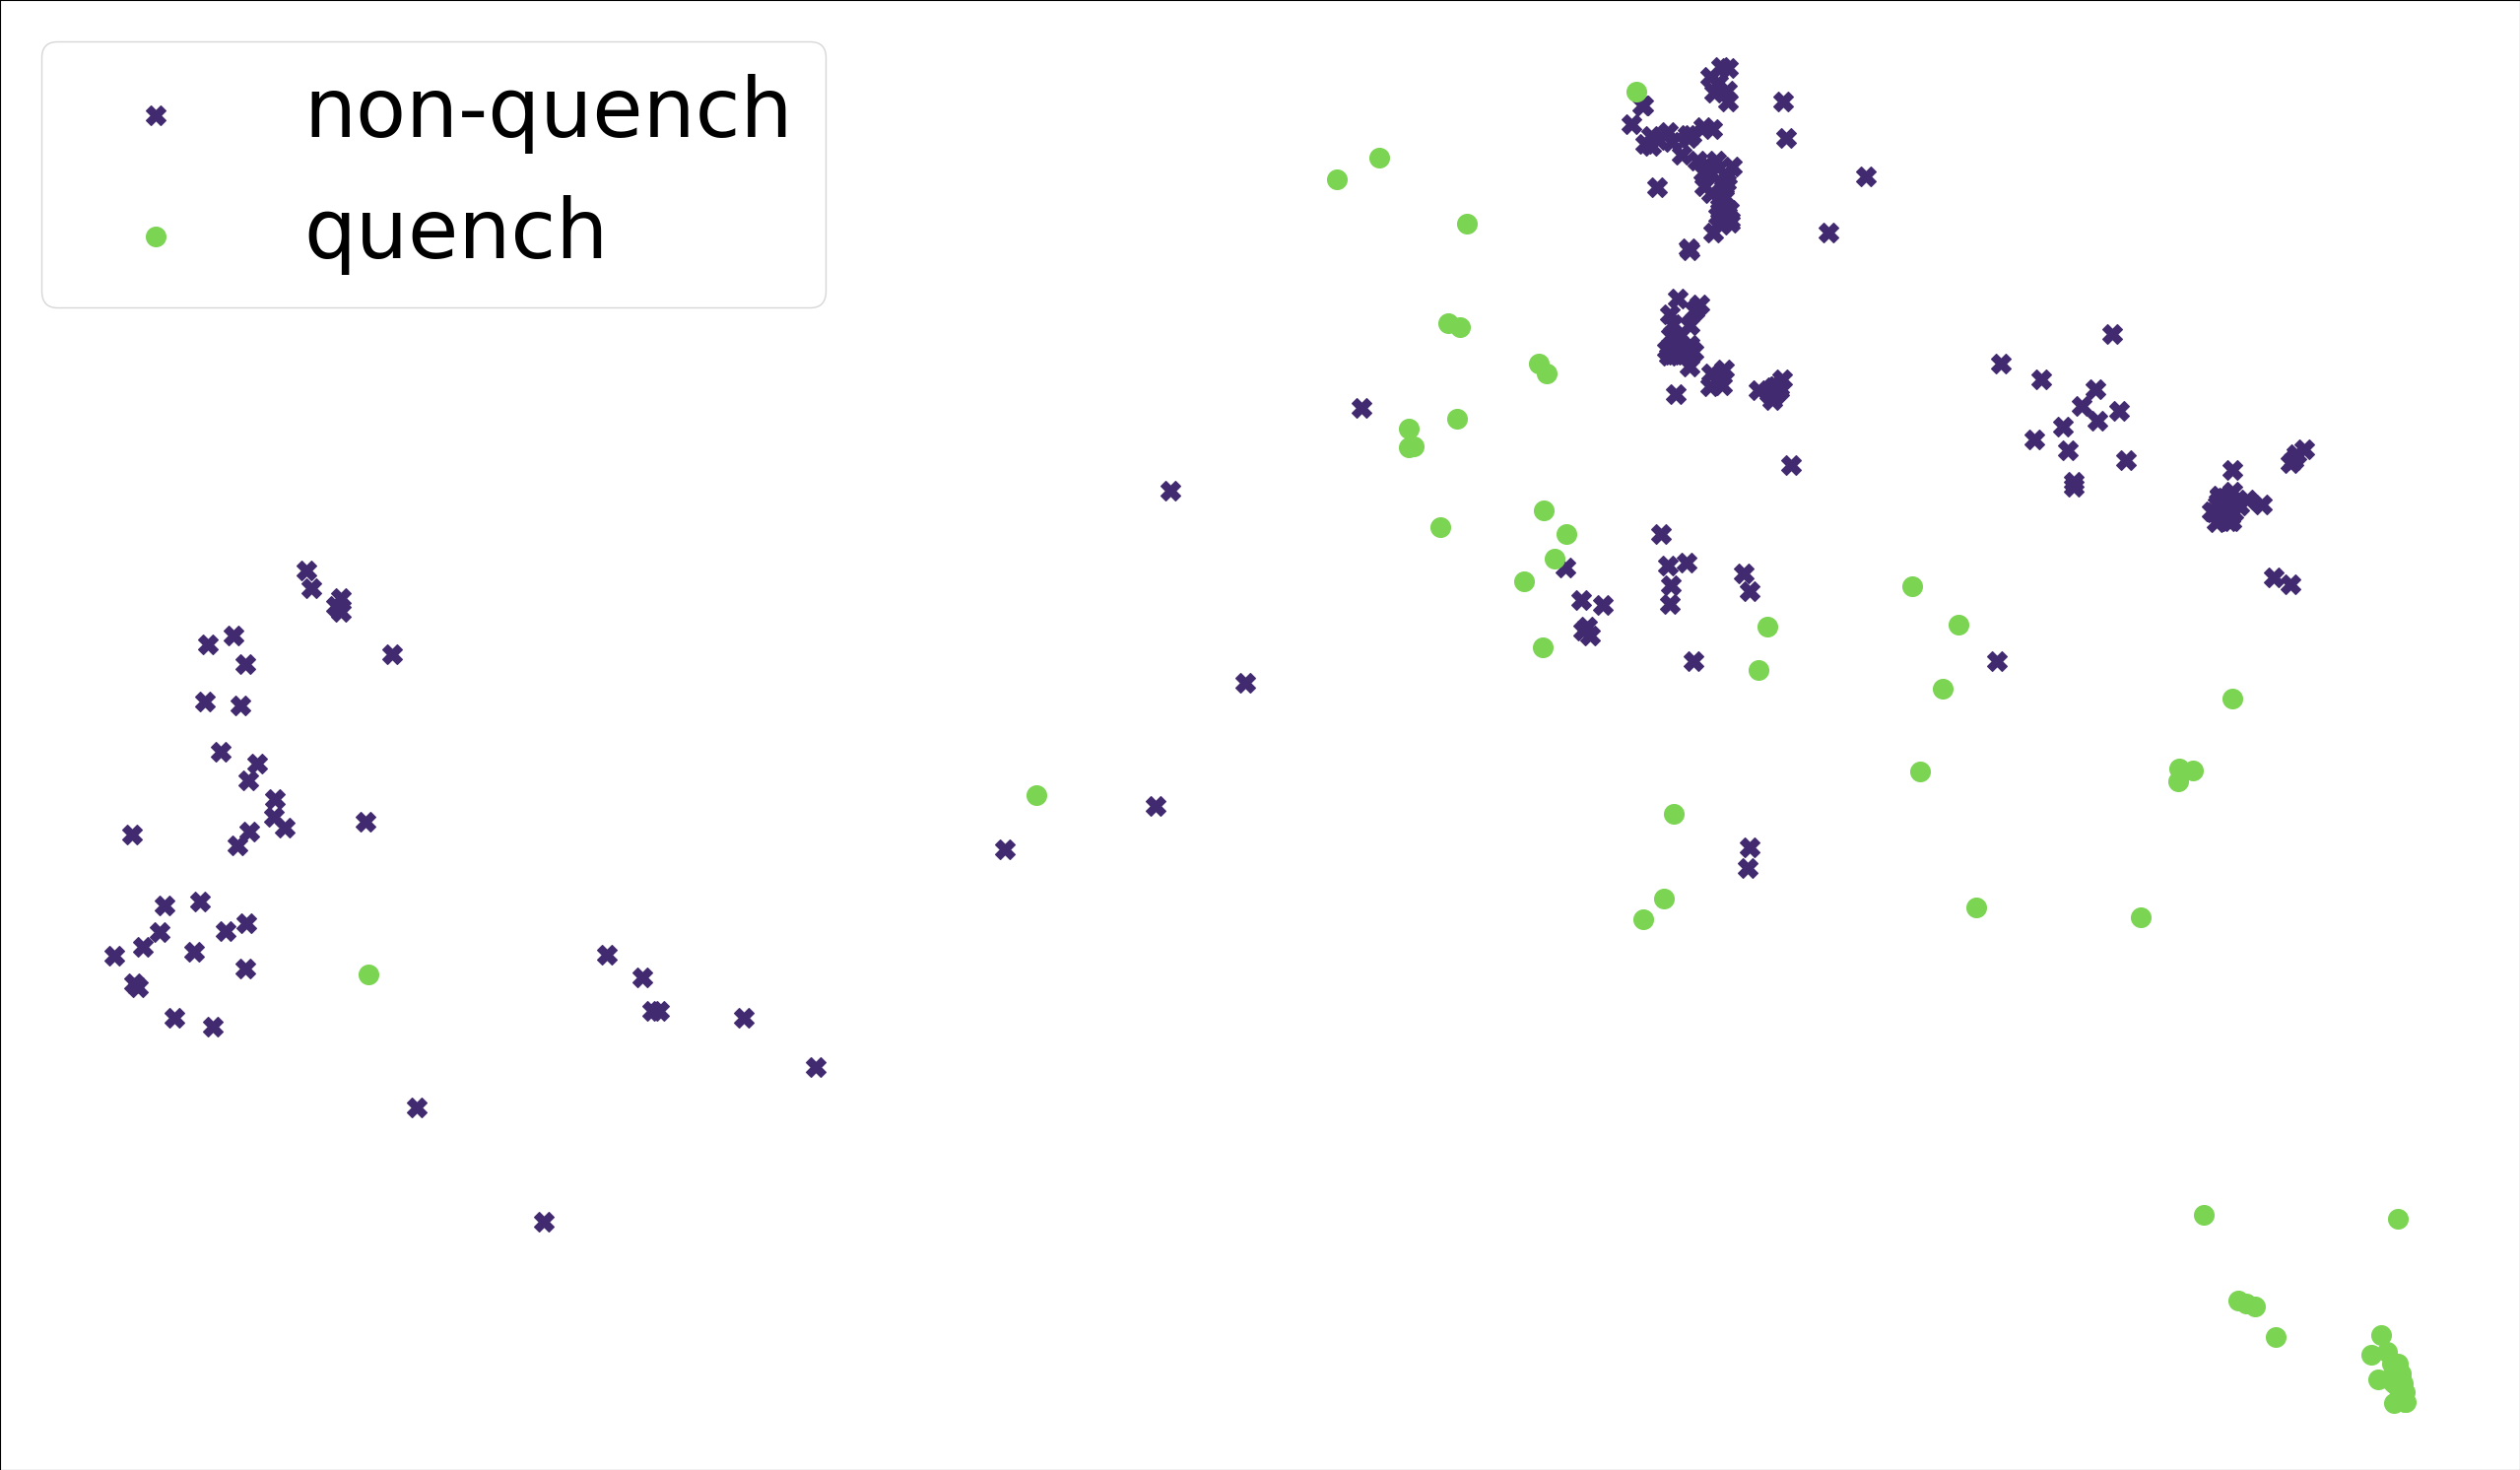
\includegraphics[width=\linewidth]{img/quench_dist_qlp/quenches_coil_0_Phi.png}
		\subcaption{}
	\end{subfigure}
	\begin{subfigure}{0.49\linewidth}
		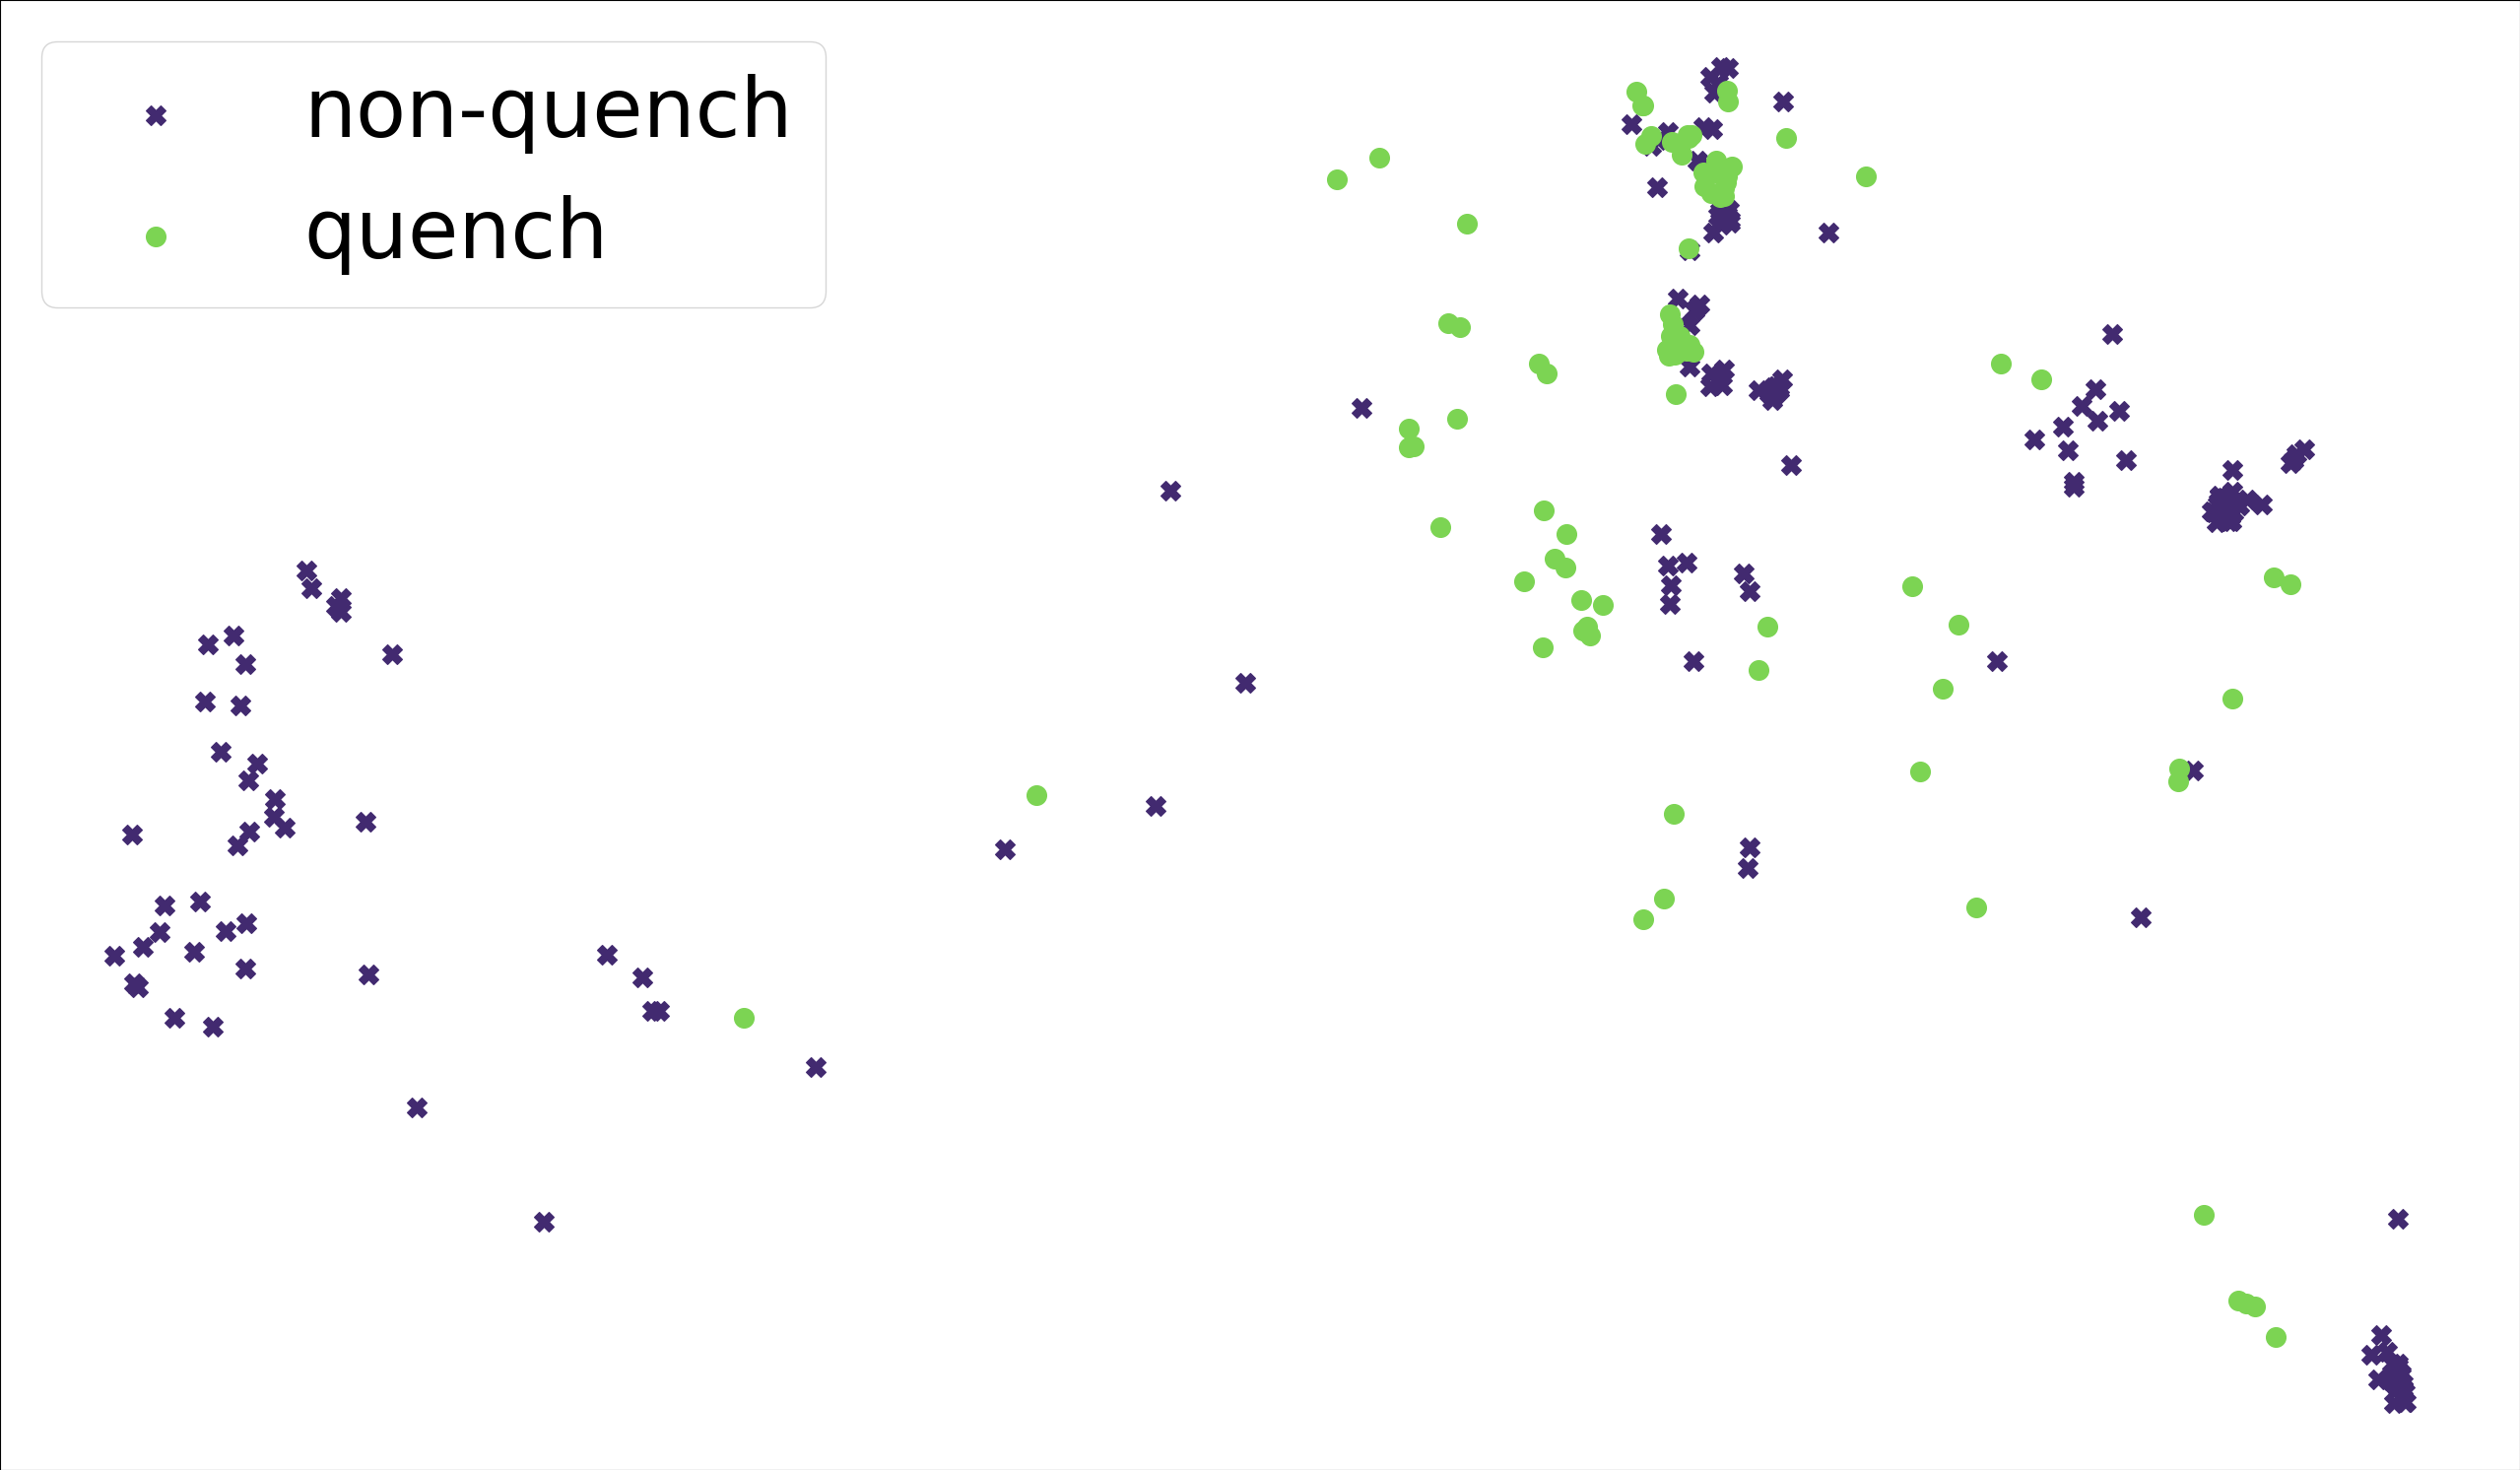
\includegraphics[width=\linewidth]{img/quench_dist_qlp/quenches_coil_1_Phi.png}
		\subcaption{}
	\end{subfigure}
	\begin{subfigure}{0.49\linewidth}
		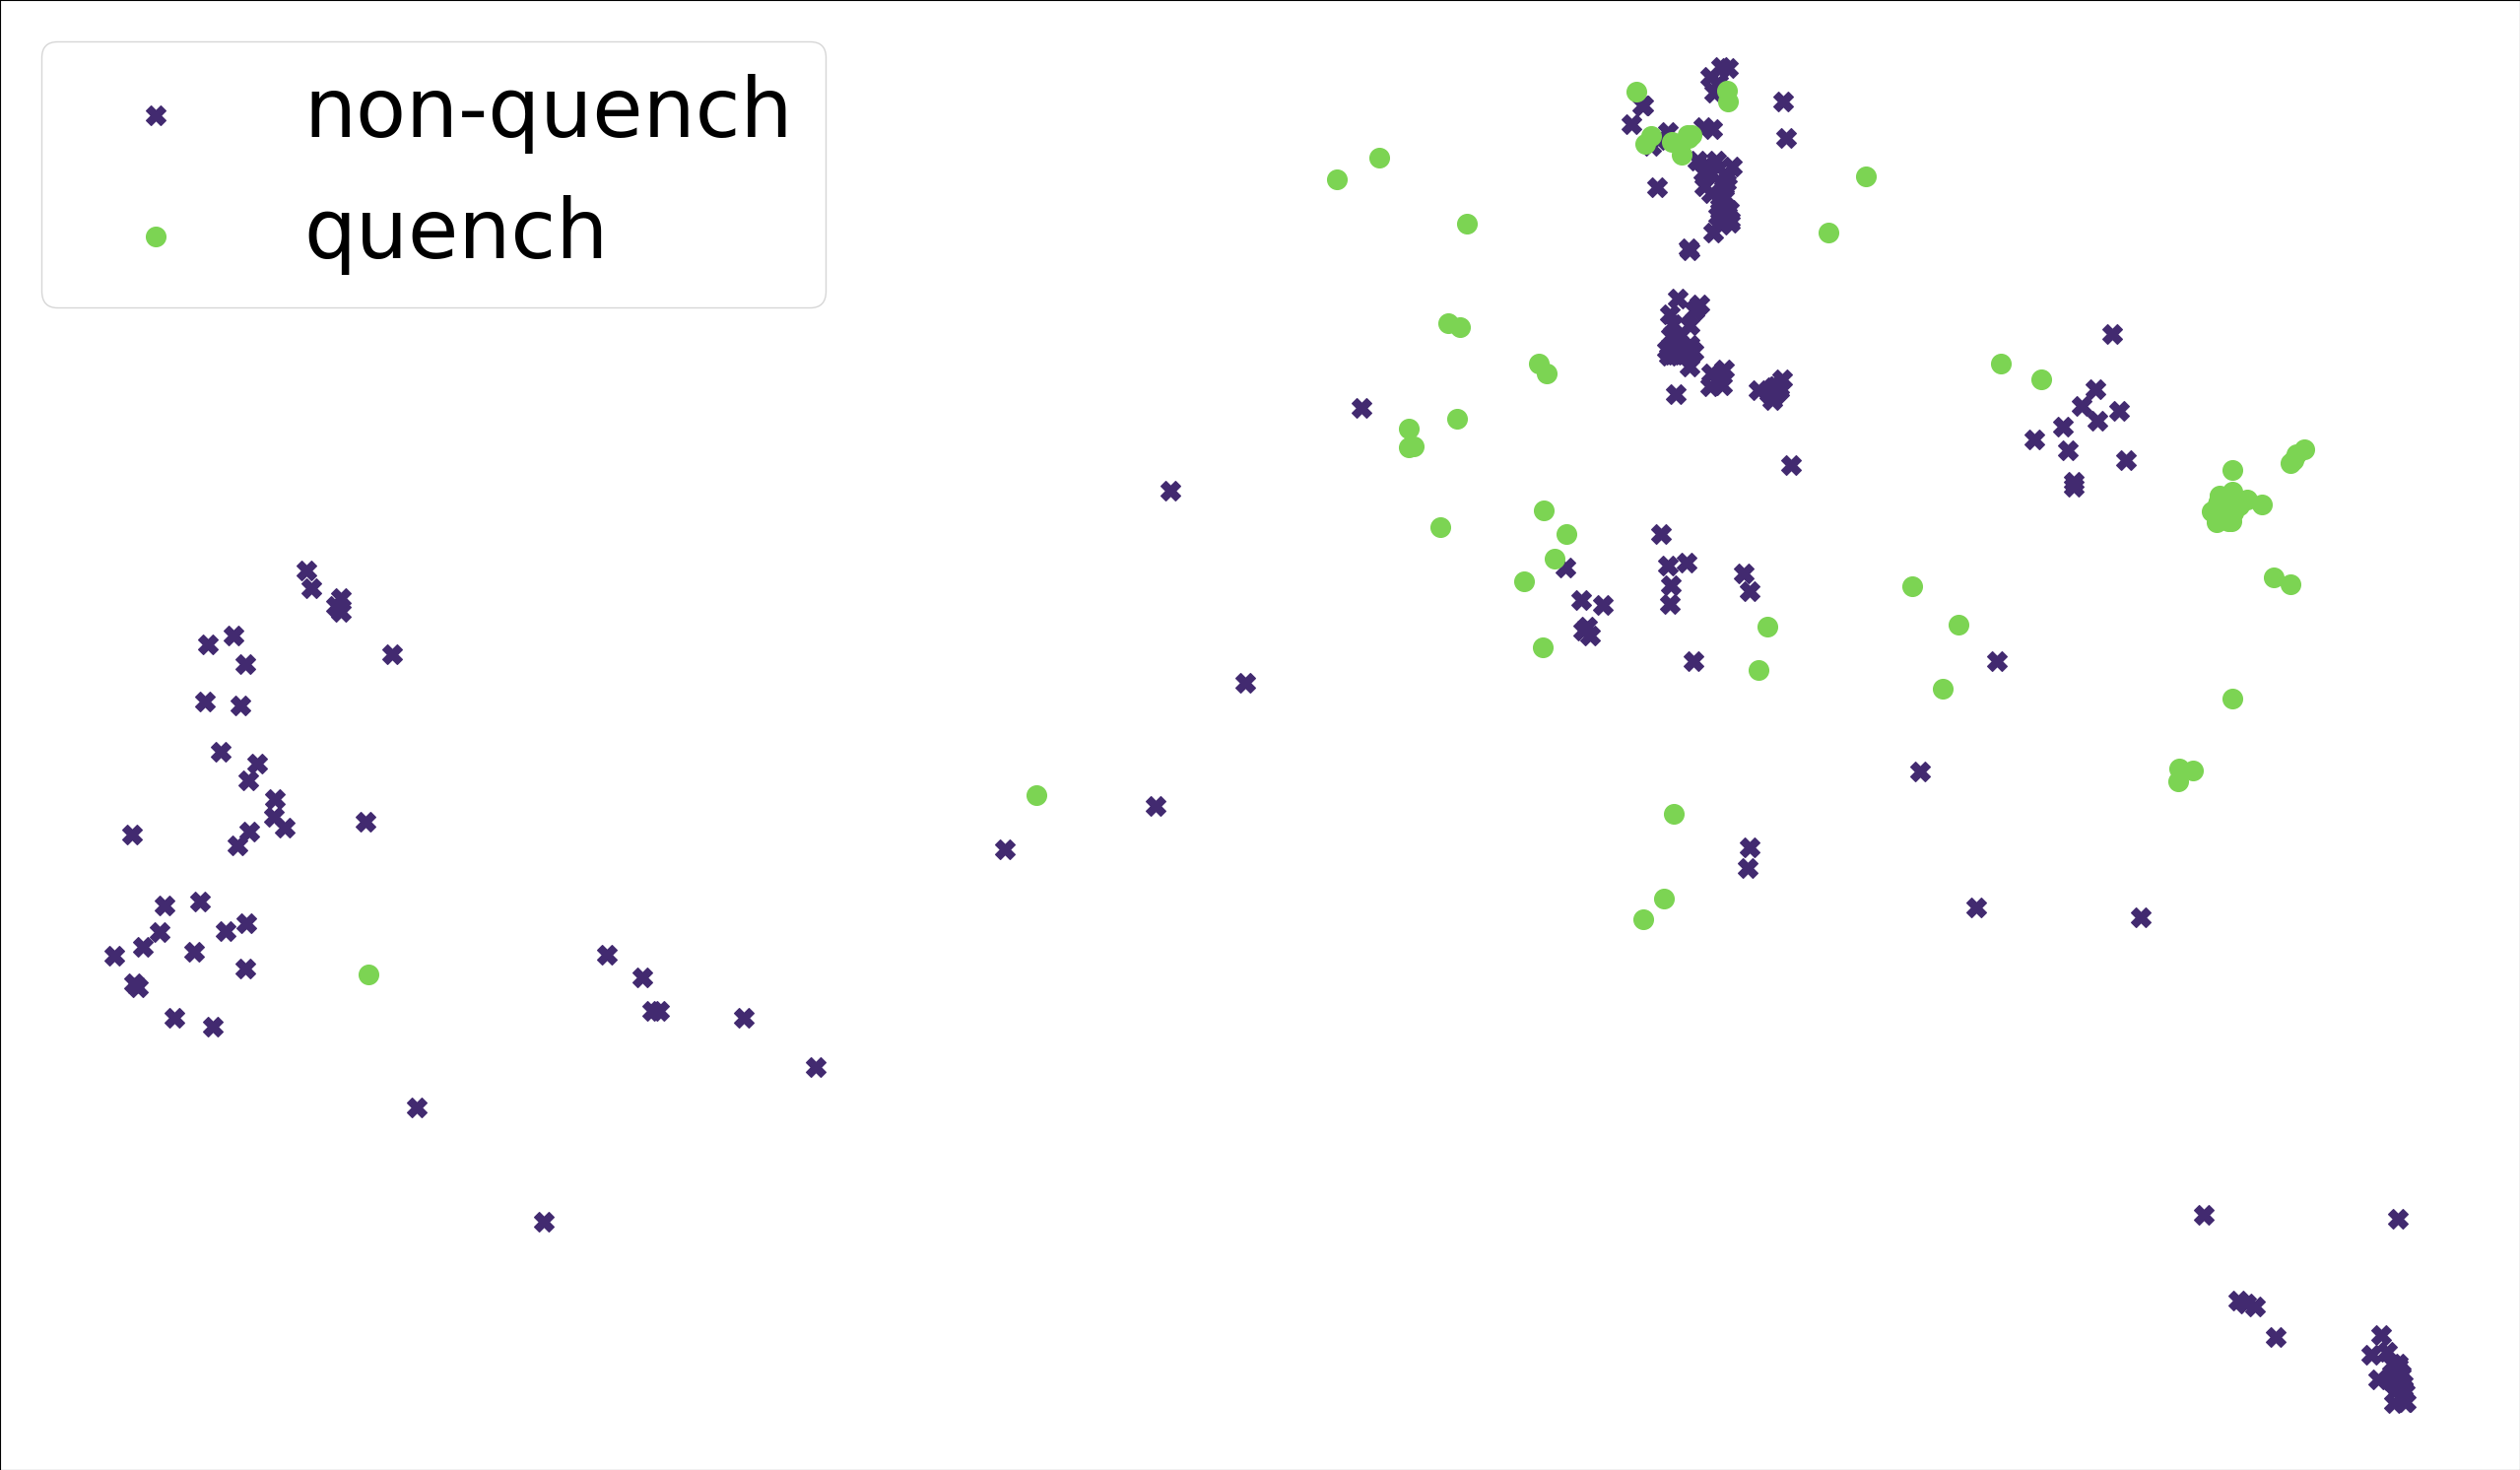
\includegraphics[width=\linewidth]{img/quench_dist_qlp/quenches_coil_2_Phi.png}
		\subcaption{}
	\end{subfigure}
	\begin{subfigure}{0.49\linewidth}
		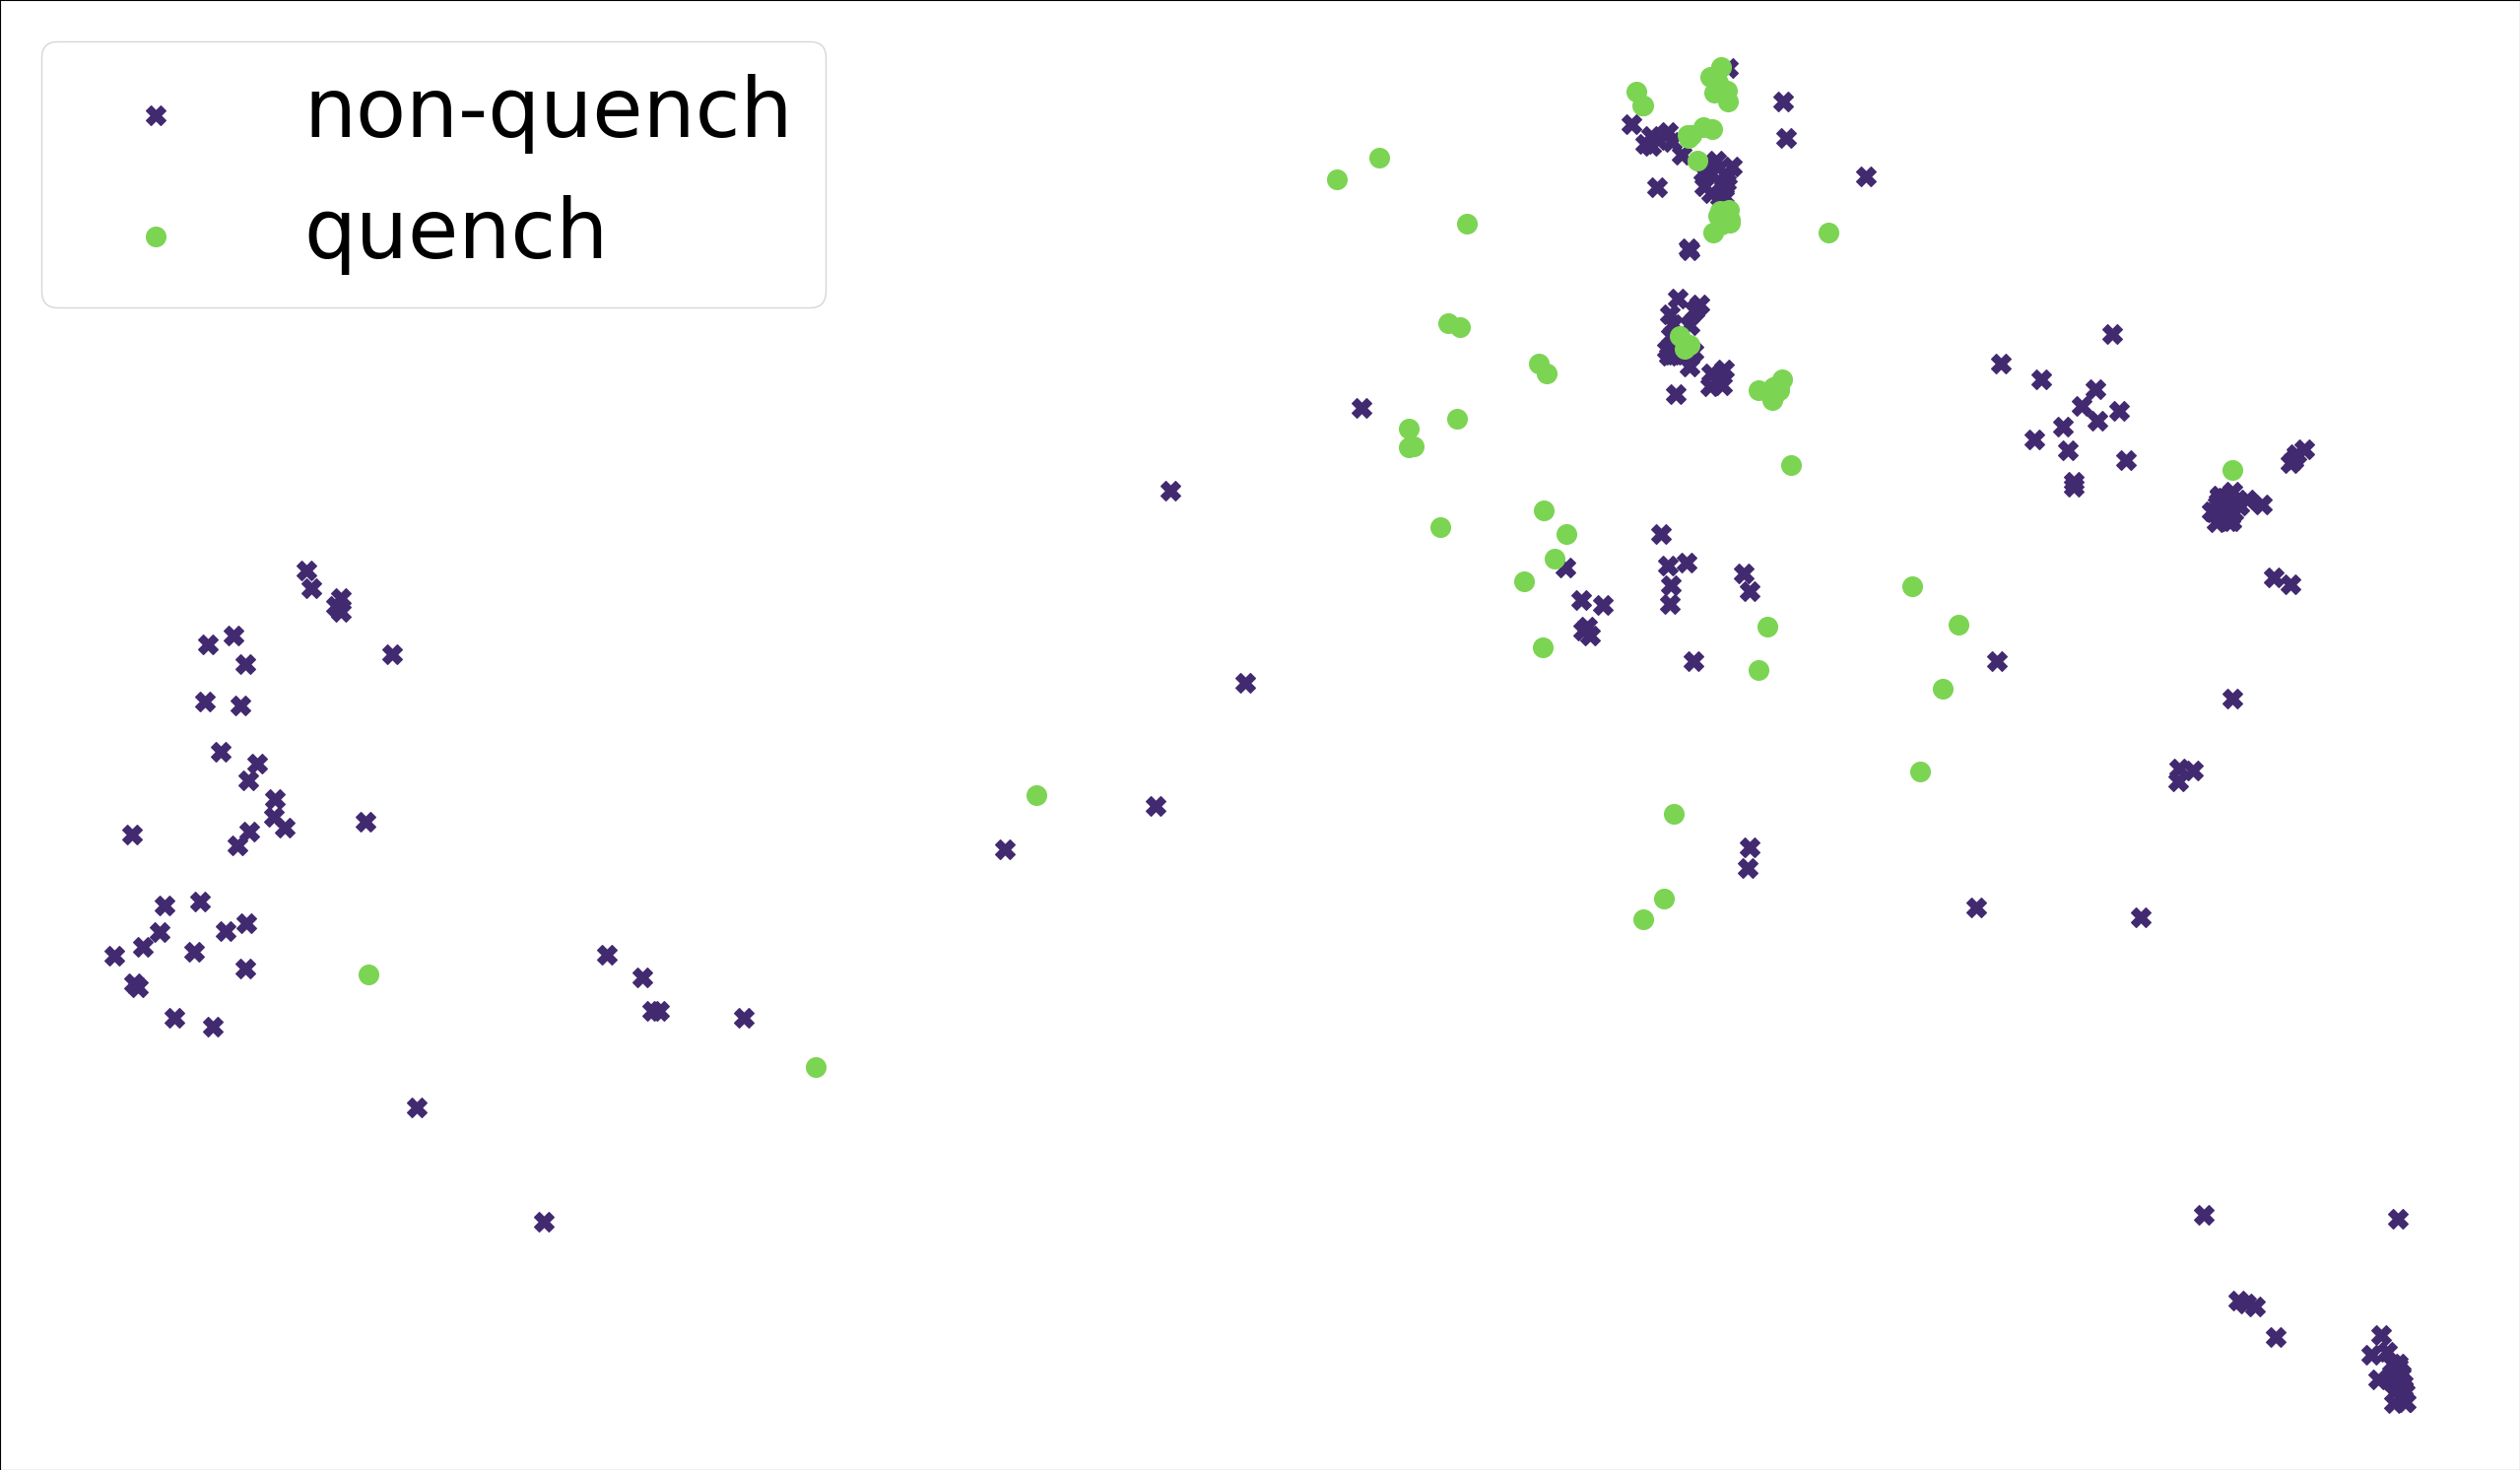
\includegraphics[width=\linewidth]{img/quench_dist_qlp/quenches_coil_3_Phi.png}
		\subcaption{}
	\end{subfigure}
	\caption{The distribution of the samples in bidimensional space after a round of \pca, for
		the \phin\ attribute. the subfigures contain different views of the same data: (a) differenciates between non-quench and single or multiple quench events, (b) highlights the distribution of quenches for coil $0$, (c) highlights the distribution of quenches for coil $1$, (d) highlights the distribution of quenches for coil $2$ and finally (e) highlights the distribution of quenches for coil $3$.}
	\label{fig:phi-coilq-dist}
\end{figure}

\section{First approaches using Clustering}

\section{Results}
We thought that a good idea to solve \qlp\ was to extend the original models used to solve \qrp. The
very first experiments we worked on included trying to solve the new problem using the
multiclass-classification version of the original models, we didn't have high expectations for this
since the new models have to predict $4$ different bits, instead of just one, making the problem
effectively much more difficult than \qrp.

As an example, we started with trees, and even if they always had maximum depth between $5$ and $10$
(therefore having a structure close to the limit of what we would consider explainable) the accuracy
was close to $60 - 70\%$. The performance were obtained by doing micro averaging, which means that
the resulting metrics are mindful of the class imbalance.

Since the performance obtained using a direct extension of trees didn't really suit our expectations
we chose to change approach: Decision trees (and the other models) have performed at a very high
level in \qrp, therefore all that we have to do to solve \qlp\ is solve \qrp\ four times (one for
each coil). We need to find new estimators, different from the ones used to solve \qrp, because they
have been trained on a single label that had a completely different analytical representation, if we
tried to use the same models to the single coils they would be trying to abstract the same pattern
from a different classification problem, which leads to very poor performance.

In the following we will retrace the steps we walked in \Cref{chp:qrp} and we will describe the best
models found to solve the problem.

\subsection{Decision trees}
As we said previously, decision trees utilized in the multiclass-classification environment provided
performance that left a lot to be desired, to counteract this we chose to reinterpret \qlp\ as a
problem in which we need to understand whether each coil has quenched, separately (therefore
solving \qrp\ $4$ different times). To keep the discussion of the performance concise we will be
discussing the structure of the best models and concentrate on the performance of the aggregate.

To evaluate the performance of the aggregate model, containing one classifier per coil, we defined a
metric named 'Hamming score' ($\hs$ in the following), which simply computes how different are the
prediction and the expected outcome.

\Cref{fig:bdts-qlp} contains the performance metrics obtained in the outer \cv\ for the best single
tree trained on each coil. The metrics are quite close to each other, with the only clear outlier
being the model trained on coil $3$.

Instead of including a plot of the various trees we condensed the most important information
in \Cref{tbl:tree-description}, all the trees described have a depth of maximum $5$ and the number
of internal nodes and leaves is always very acceptable, while the trees built on \an\ remain on the
smaller side, the trees built for coil $1$ and $3$ are larger (with the one built on \cnmod\ being
the largest at $15$ total nodes), despite their structure being more complex, these trees struggle
compared to the ones trained on sub-views of \an.

\begin{figure}[!ht]
	\centering
	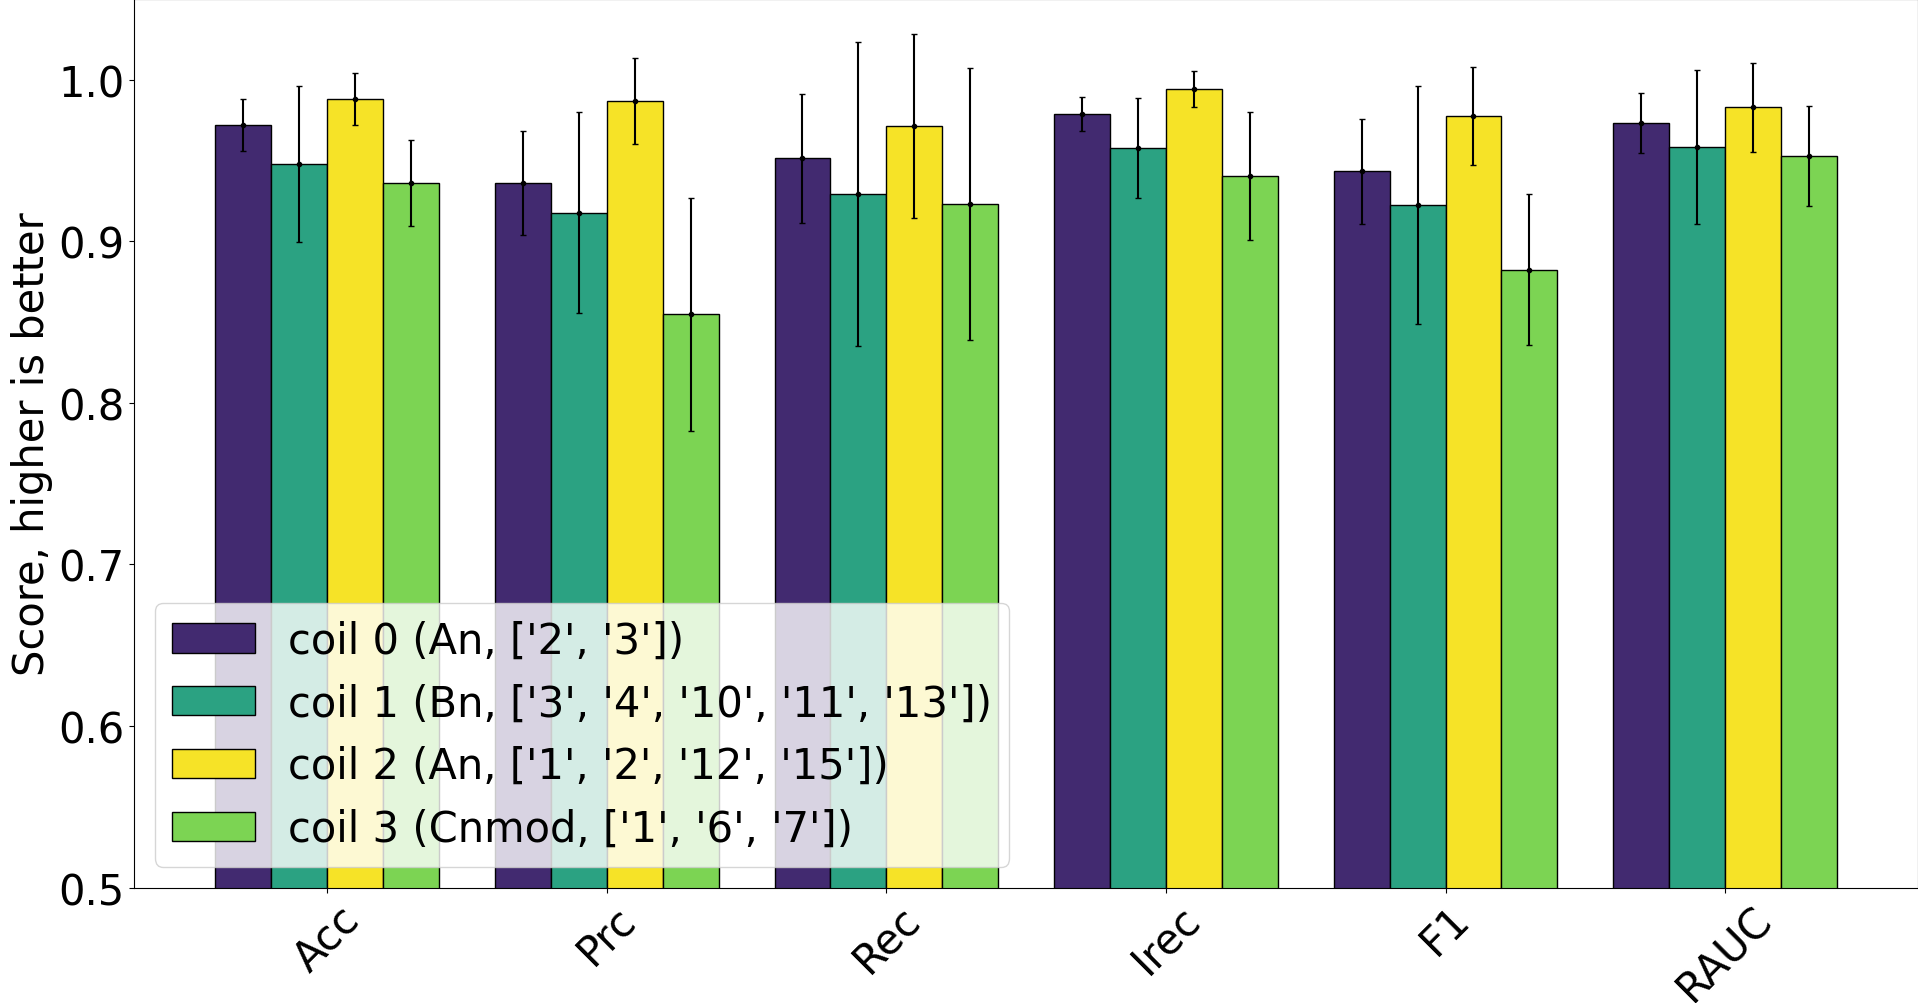
\includegraphics[width=\linewidth]{img/best_dts_qlp.png}
	\caption{Comparing the performance of the best model built on every coil, independently of
		the dataset used.} \label{fig:bdts-qlp}
\end{figure}

\begin{table}[!ht]
	\caption{Description of the best \dt\ for every coil.}\label{tbl:tree-description}

	\bigskip
	\setlength{\tabcolsep}{6pt}
	\centering
	\begin{tabular}{lcccc}
		\toprule
		\textbf{}                           & \textbf{Coil 0}  & \textbf{Coil 1}          & \textbf{Coil 2}          & \textbf{Coil 3}
		\\
		\midrule
		\textsc{attribute}                  & \an              & \bn                      & \an                      & \cnmod                          \\
		\multirow{2}{*}{\textsc{harmonics}} & \an[2], \an[3]   & \bn[3], \bn[4], \bn[10], & \an[1], \an[2], \an[12], & \cnmod[1], \cnmod[6], \cnmod[7] \\
		                                    &
		                                    & \bn[11], \bn[13] & \an[15]                  &                                                            \\
		\textsc{depth}                      & 3                & 5
		                                    & 3                & 5                                                                                     \\
		\textsc{N internal nodes}           & 4                & 5
		                                    & 3                & 8                                                                                     \\
		\textsc{N leaves}                   & 5                & 6
		                                    & 4                & 7                                                                                     \\
		\textsc{N nodes}                    & 9                & 11
		                                    & 7                & 15                                                                                    \\
		\bottomrule
	\end{tabular}
\end{table}

In \Cref{fig:dt-qlp-hs}, we plotted the performance of the aggregate model, which are obtained as we
did when testing \tas\ for \qrp: A run of $5$-fold \cv\ and we computed the number of errors done by
the ensemble on the $4$ bit array. On average the classifiers makes $2$ errors or less, since the
minimum accuracy is $0.5$, averaging the performance of all the folds we get a final Hamming score
which is $0.95$ and with a standard deviation of $0.024$. Testing the performance of the aggregate
on the final blind-test, if we average the Hamming score on the $29$ samples, we get higher
performance on average $0.966$ and a higher standard deviation $0.086$ (this difference is probably
due to the lower amount of data we are averaging on), the trained aggregate makes $4$ single errors
on the $116$ total labels that it needs to predict.

Our supposition at the moment is that finding a better model for coil $3$ would make the performance of
the ensemble better because, while we have been saying that the model is an aggregate of trees, no
aggregation is happening (like in the case of \tas) apart from inserting the predicted bits in a
prediction array, therefore the sub-models are not helping each other and 'covering for each other'.

\begin{figure}[!ht]
	\centering
	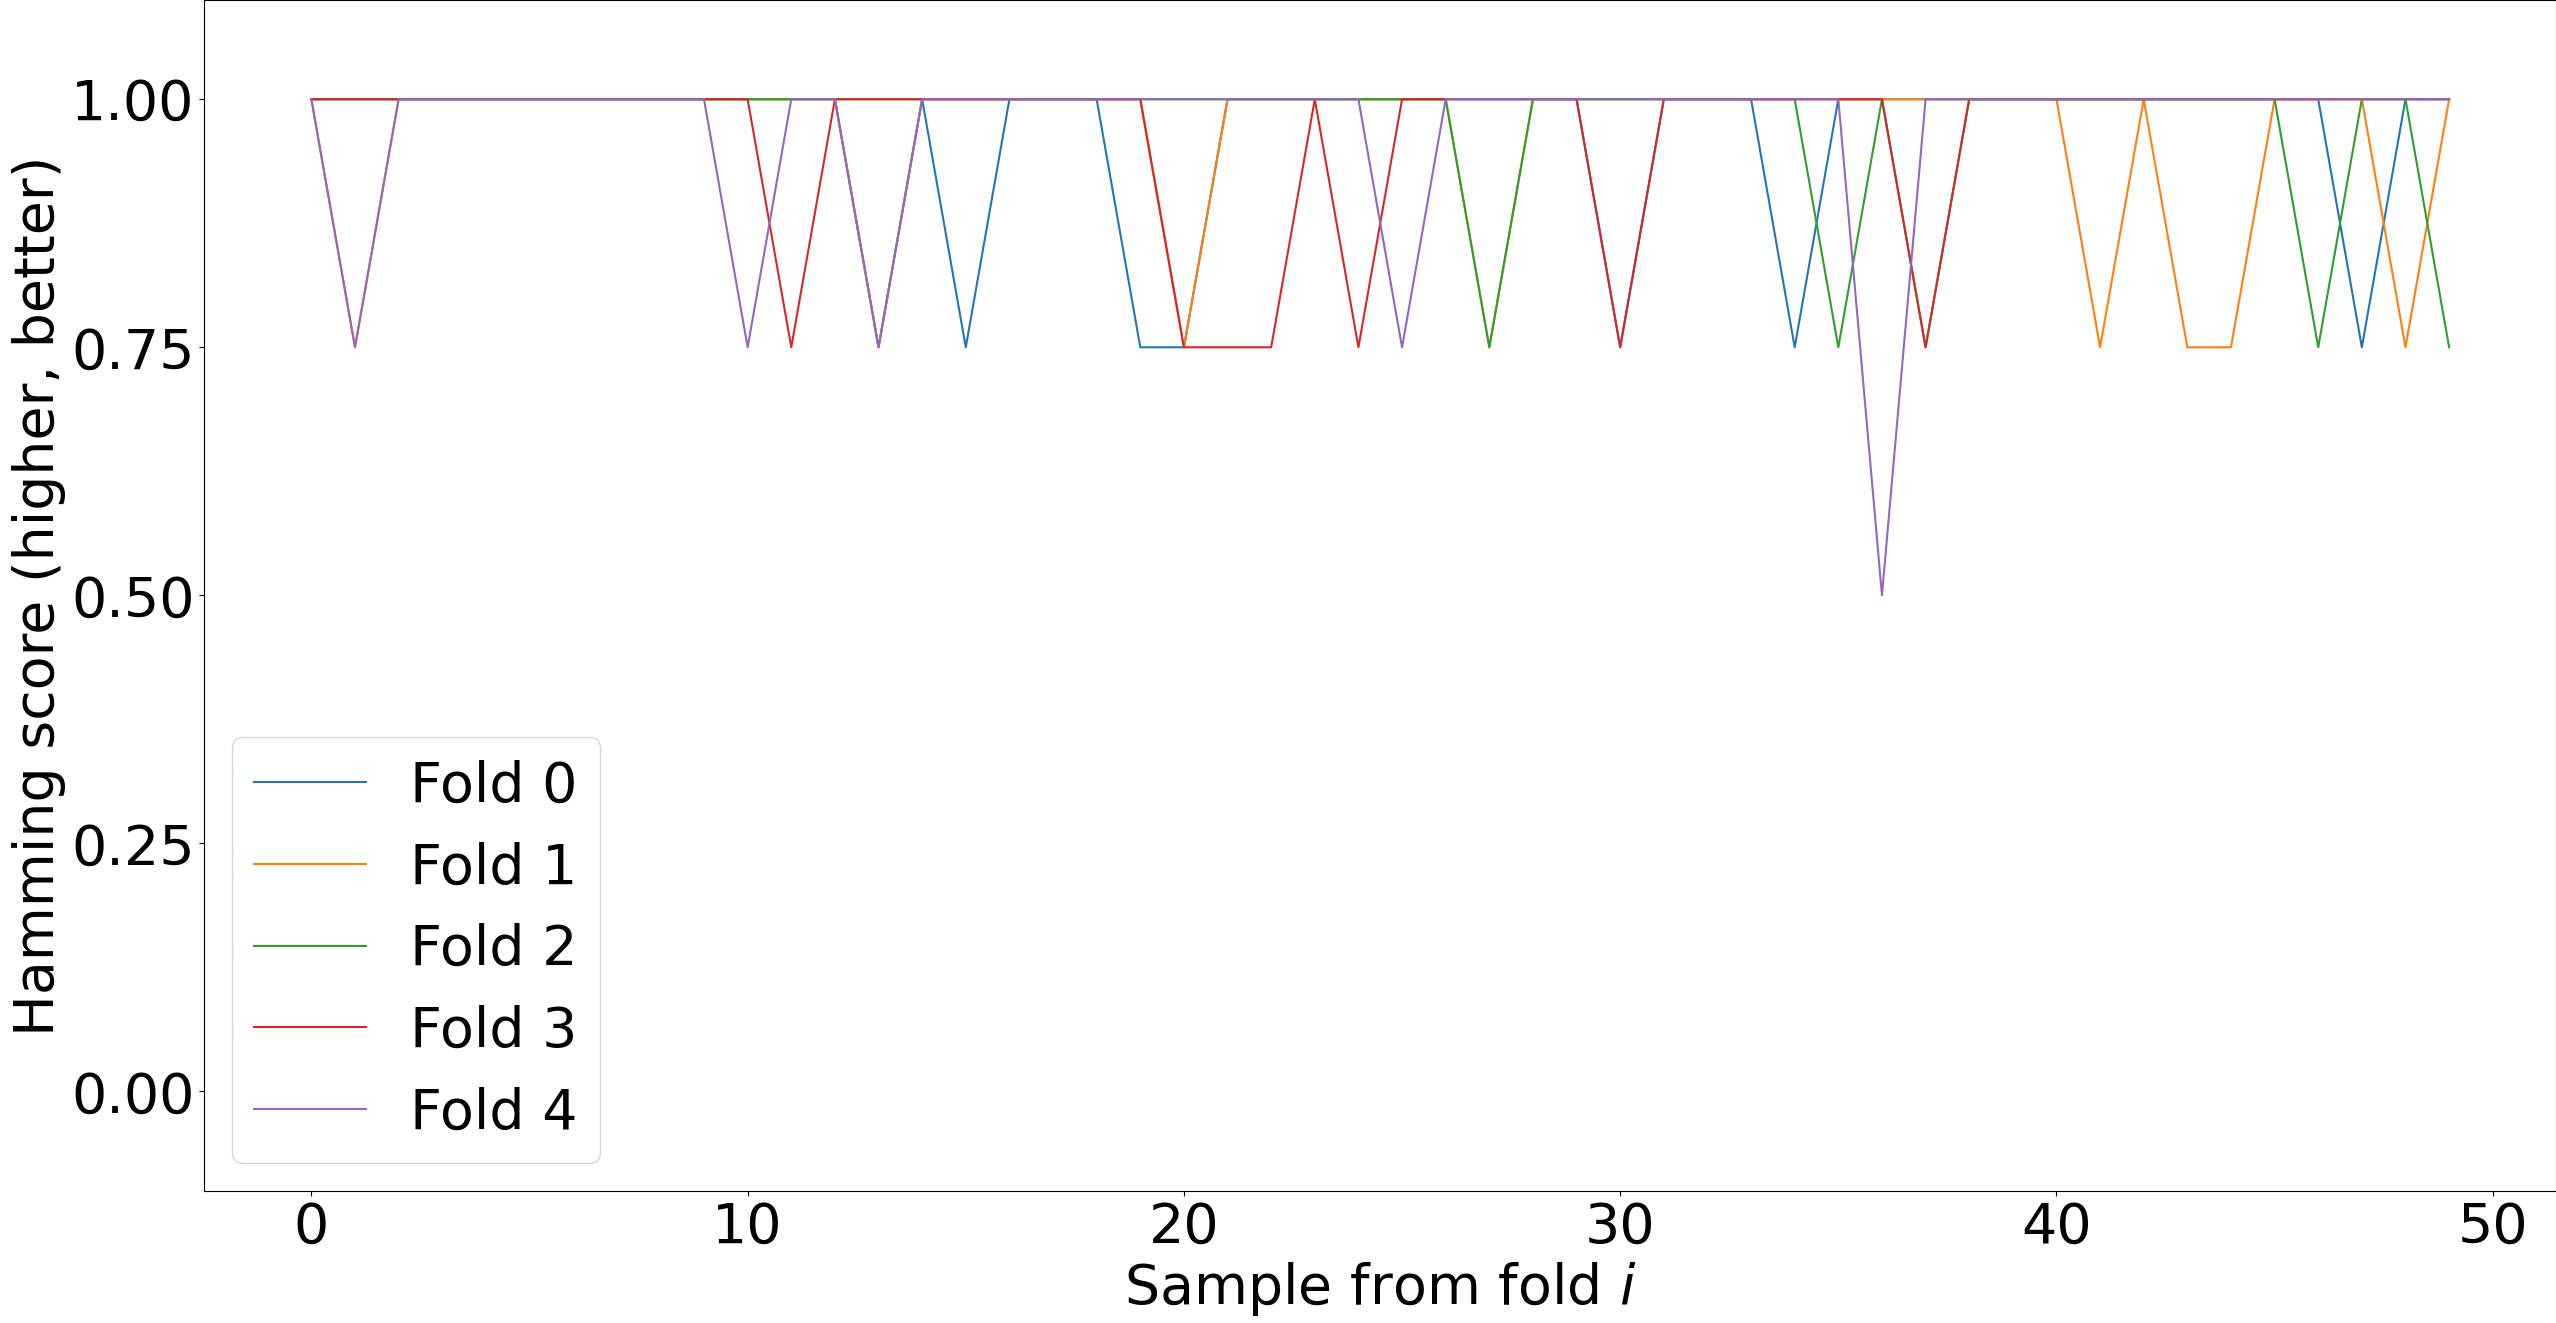
\includegraphics[width=\linewidth]{img/best_dts_hs.png}
	\caption{The Hamming score computed on every fold (for the $50$ samples therein contained), the lower reaching is the line the lower is going to be the accuracy.} \label{fig:dt-qlp-hs}
\end{figure}

\subsection{Random forests}
Similarly to what we just did for \dts\ we also evaluated the performance of a model containing one
single forest per coil, we expected higher performance compared to the ones just obtained on \dts,
at the expense of a lower explainability.

\Cref{fig:brfs-qlp} shows the performance for the best rfs built on a mix of different attributes
(each taken in its entirety), as we can see the performance metrics are better, but we are not far
off from the numbers obtained in the case of \dts\ (see \Cref{fig:bdts-qlp}), also, our weakest
learner, the one built for coil $3$ is not much worse than the proposed random forest, while being
much simpler than the alternative.
\begin{figure}
	\centering
	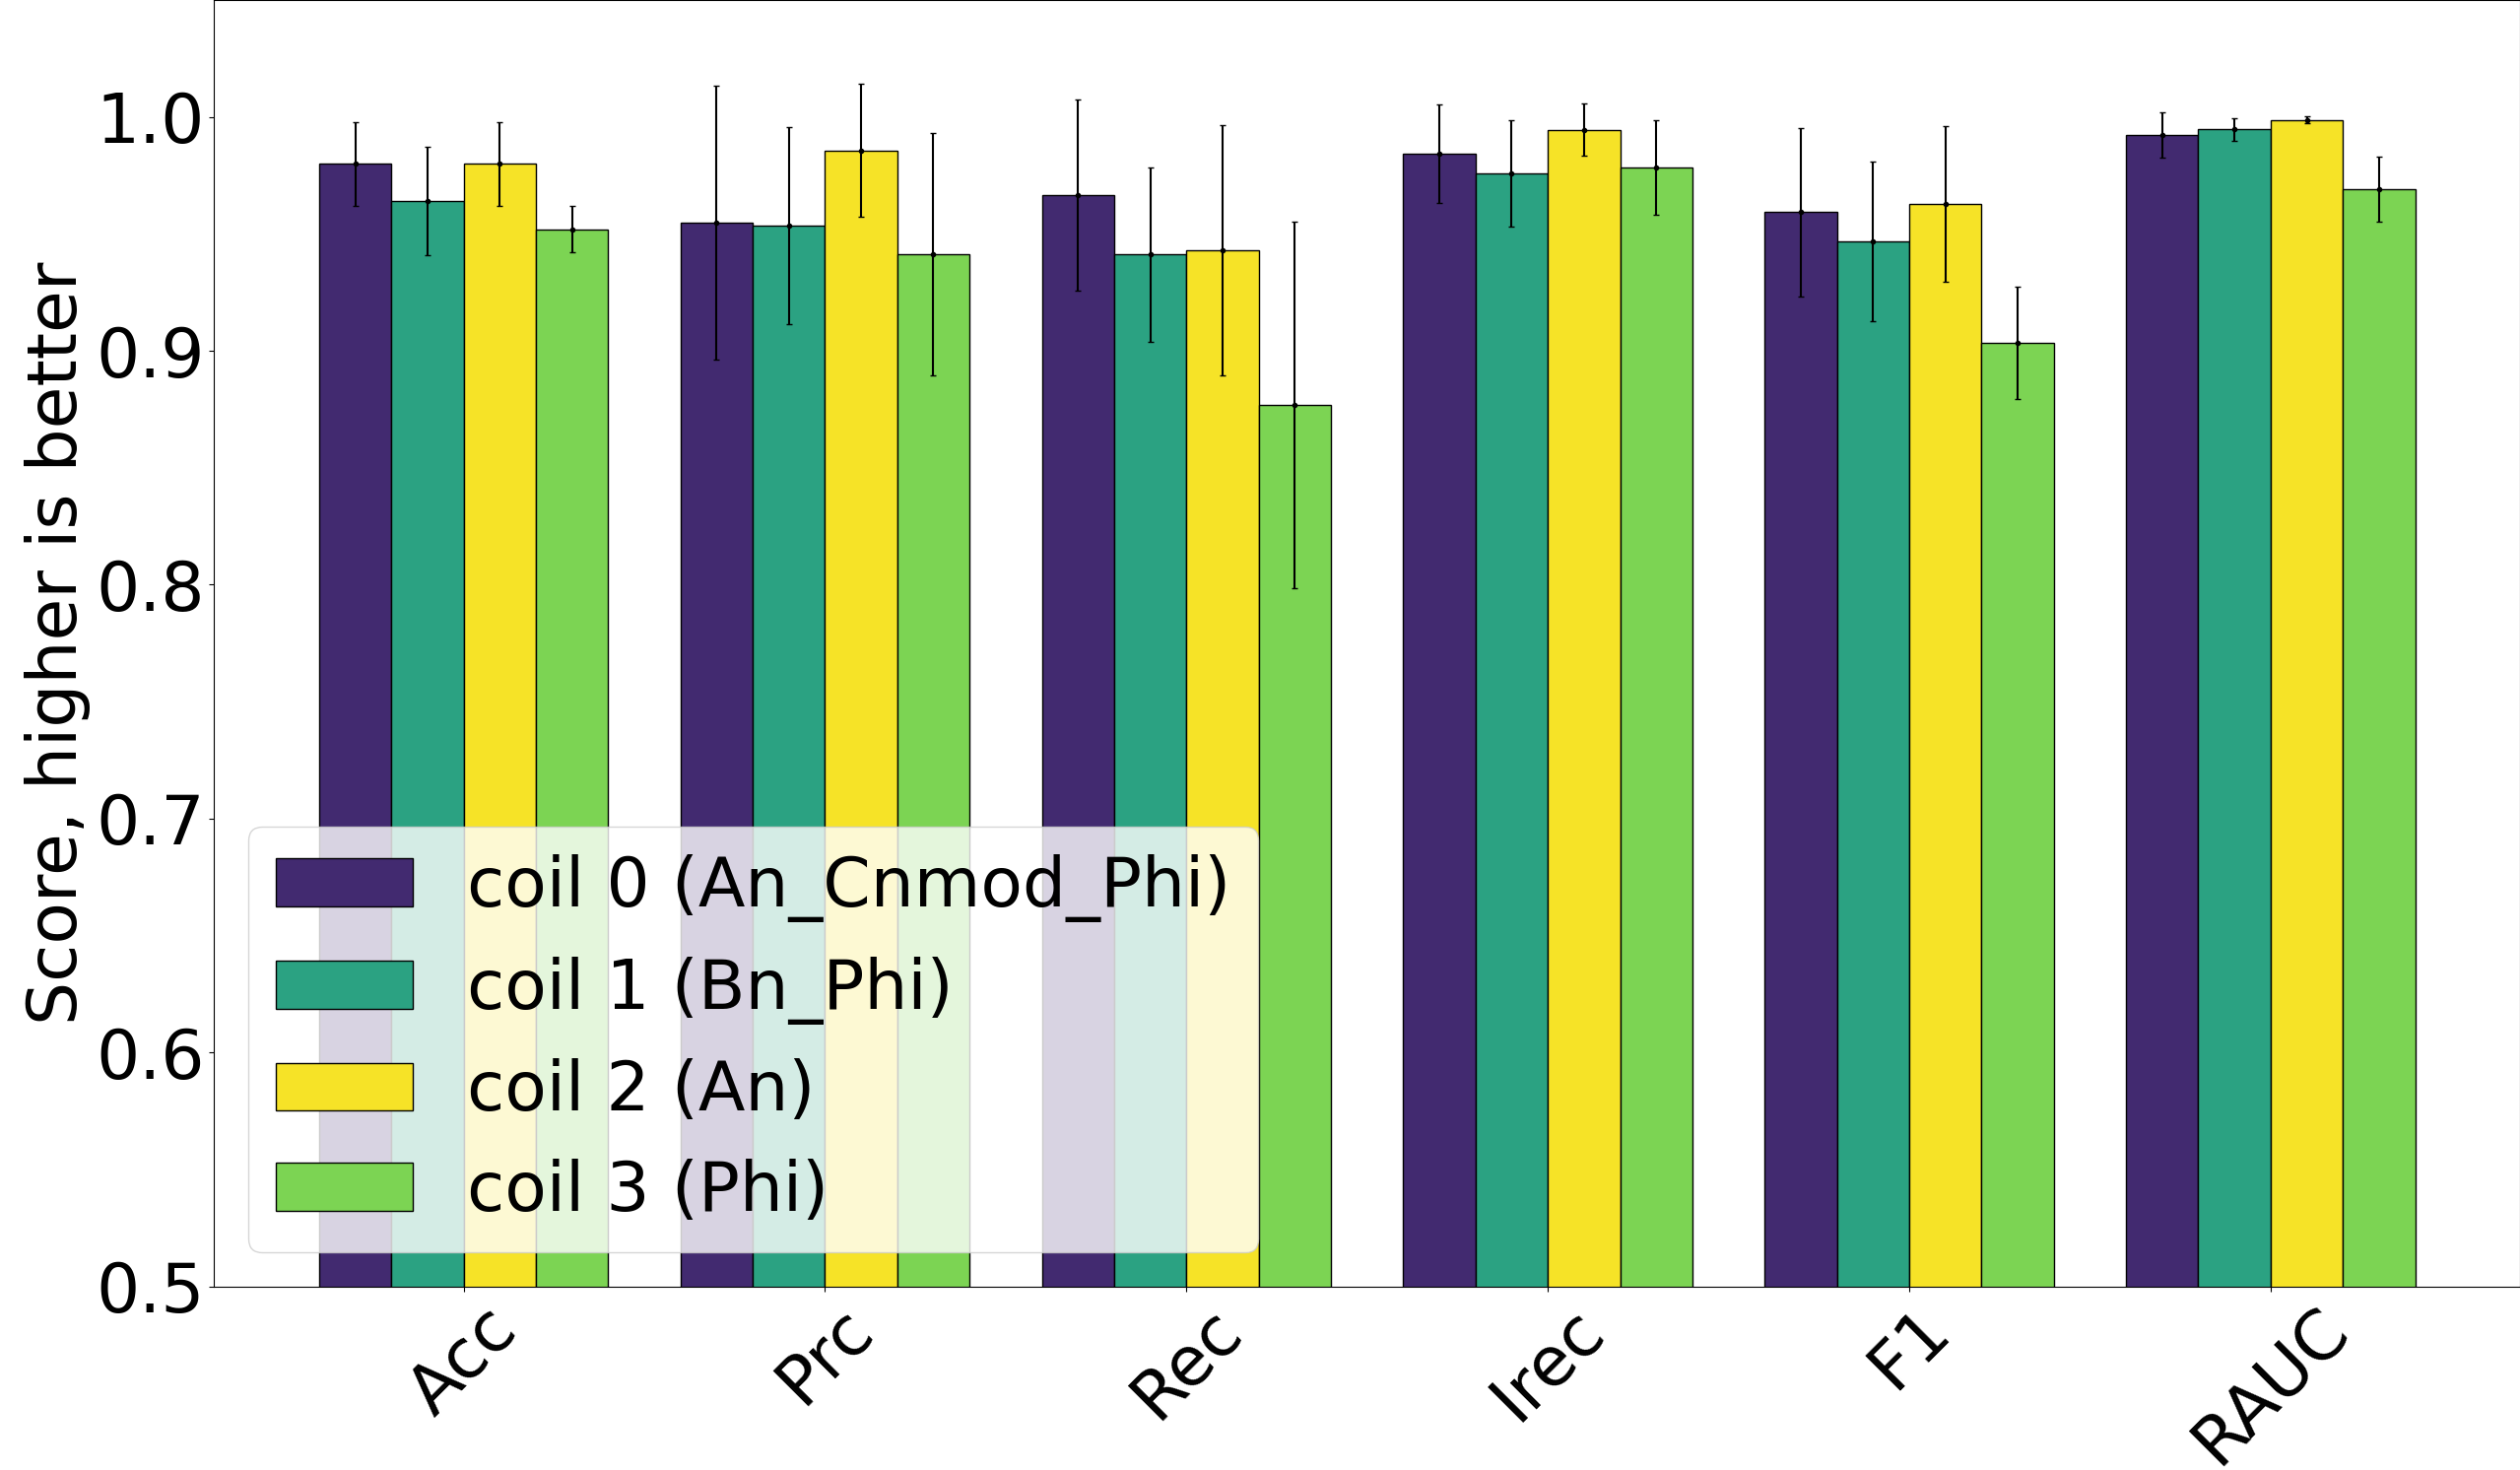
\includegraphics[width=\linewidth]{img/best_rfs_qlp.png}
	\caption{The best random forest trained on a sub-view or mix of sub-views, for every coil,
		since all of the models have been plotted without indicating the harmonic content it means
		that they are using full attributes.}\label{fig:brfs-qlp}
\end{figure}
The \rfs\ in figure contain respectively $5, 10, 10$ and $10$ trees. As we have already said
previously, while trees have a high level of explainablilty, trying to interpret a structure
containing $10$ of them is certaintly a complex task, and I would consider it explainable only on
paper. This is why, for all intents and pourposes, while we provide the results for the Hamming
score in the following, we decided to not follow this lead too much, since it would mean having an
excessive amount of models to consider at the same time.

While the trees for the first three forests are, overall, quite simple (not too deep), contained in
the number of leaves and nodes, the last forest contains complex trees with many layers ($4$ on
average), many internal nodes and leaves. Seeing the complexity of this last tree it's evident that
the forest approach would not be feasible even in an hybrid approach based on both three trees for
the first three coils and an \rf\ for the last one.

Since \rfs\ are more complicated than we would like we avoided the calculation of the Hamming
score, also because the performance are good but not good enough to make us consider their use when
compared to the simpler \dts.

\subsubsection{Support Vector Classifiers}
If we analyze the benchmark model, and we train it without constraints (one or more sub-views for
different datasets), the results are that we can aim at a very high level of performance if we
forget about explainability. Performance have been plotted in \Cref{fig:bsvcs-qlp}, the metrics were
taken from the outer \cv\ loop and the models chosen were the best for each specific coil.
\begin{figure}[!ht]
	\centering
	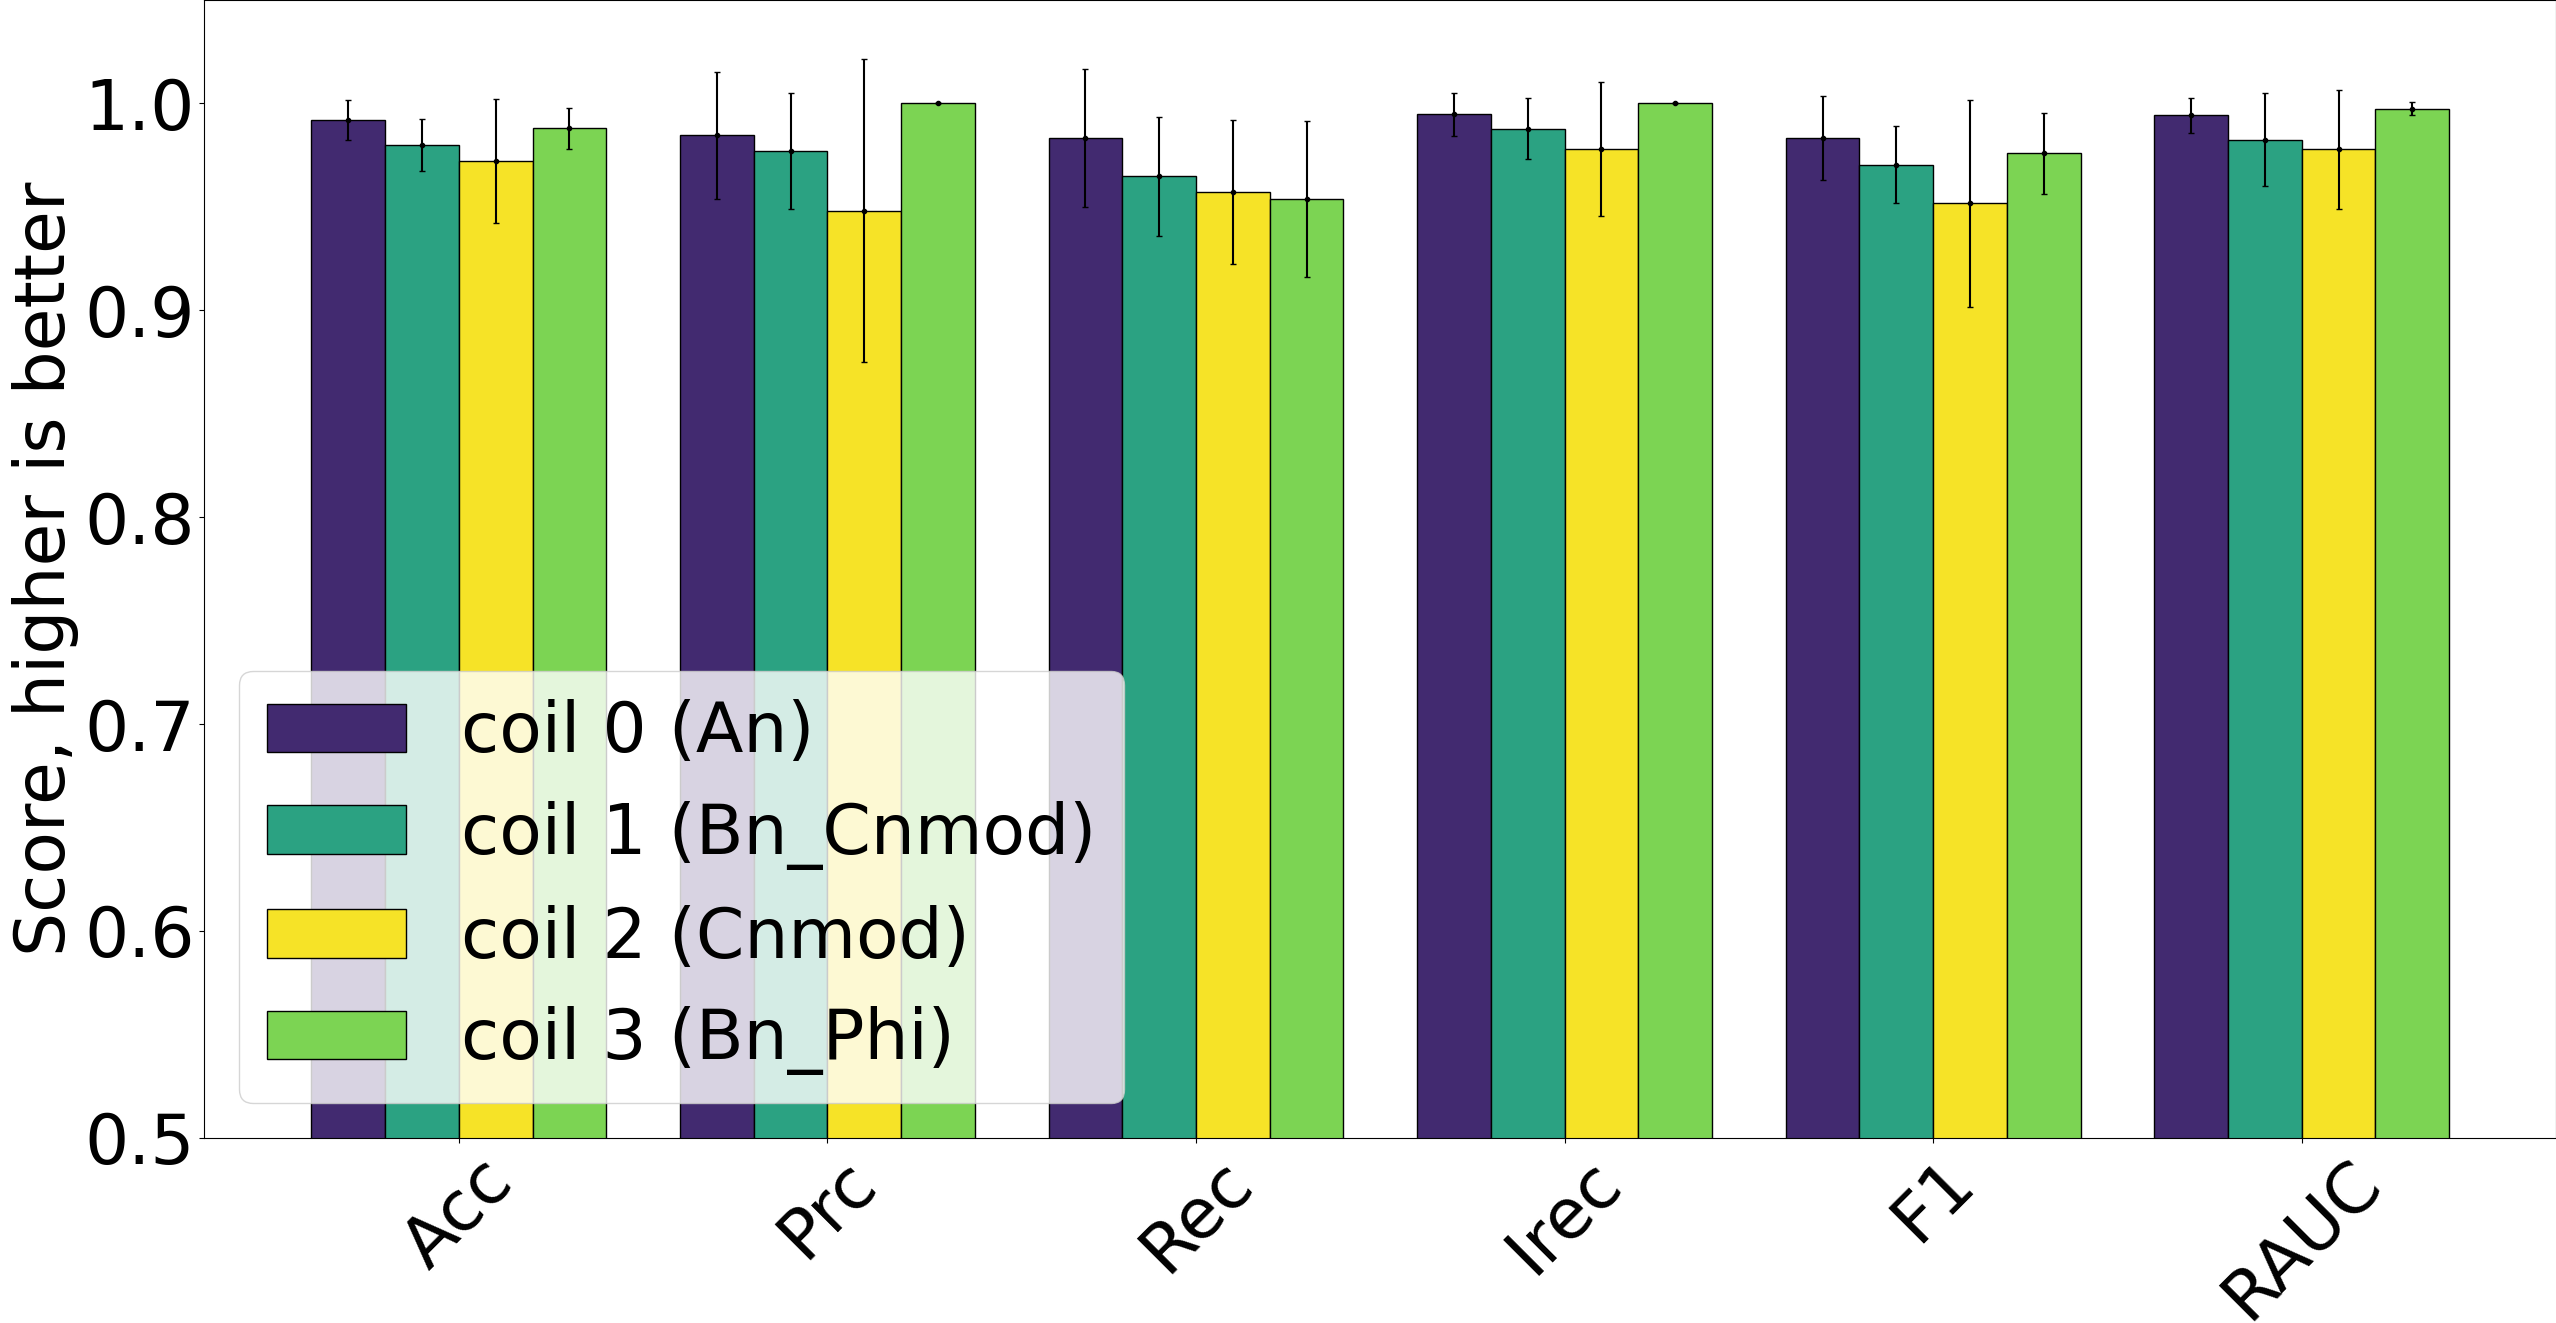
\includegraphics[width=\textwidth]{img/best_svcs_qlp.png}
	\caption{Performance metrics for the best \svcs\ trained on every coil, all attributes
		have been taken with their full harmonic content.} \label{fig:bsvcs-qlp}
\end{figure}
There are a couple of very interesting takeaways:
\begin{itemize}
	\item The best \svc\ trained on coil $0$ is based on attribute \an. This is exactly what we
	      expected since the very beginning of this chapter.
	\item The best models for coils $1$ and $3$, were trained on \bn\ and another dataset (\cnmod\ for $1$
	      and \phin\ for $3$). This is interesting for two reasons:
	      \begin{inparaenum}[(i)]
		      \item \bn\ is actually the best attribute for the two coils, as we saw in the analysis
		      we did in the beginning of the chapter,
		      \item the \svc\ trained on the sole \bn\ performed worse than the alternatives. This
		      lead us to believe that, like in the case of \qrp, \bn\ alone doesn't contain
		      enough information
	      \end{inparaenum}.
	\item Interestingly, while \cnmod\ didn't perform well enough in our tests on trees for coil
	      $2$, in the case of \svc\ the model was picked over \an.
\end{itemize}
Evidently, the ceiling of performance is still very high, and we can still find ways to get closer
to the performance of our benchmark model.








